\documentclass[11pt]{article}
\usepackage[margin=1in]{geometry}
\usepackage{booktabs}
\usepackage{amsmath}
\usepackage{amssymb}
\usepackage{graphicx}
\usepackage{xcolor}
\usepackage{caption}
\usepackage{capt-of}
\usepackage{tikz}
\usetikzlibrary{arrows.meta}
\title{LoCoBench: Logical Coherence Score Evaluation\\
\large Gold-relation and mined arms on generated items}
\author{FactReasoner --- LoCoBench evaluation}
\date{\today}


\begin{document}

\maketitle

\section{Setup}

This report evaluates the Logical Coherence Score (LCS) pipeline on the \textbf{70 generated items} of \texttt{locobench-claude-5-test}. Unlike the mining experiments, relations are \emph{not} mined by a model here: each item already carries its inter-atom relations as gold labels, and those labels are compiled directly into the coherence MRF. No LLM is involved, so every number below is deterministic and reproducible offline (Merlin is the only subprocess).

\paragraph{Atom priors.} An atom's unary factor is $[1-\pi_i, \pi_i]$ with $\pi_i = 0.9$ when the item marks the atom \texttt{factual} and $\pi_i = 0.1$ when it does not. The coherence MRF therefore starts from the corpus's own factuality labels --- the label-driven analogue of the two-stage model, where stage~1's posterior marginals play this role. Hard $1/0$ priors are deliberately avoided: they would zero out worlds and make several readouts degenerate.

\paragraph{Edge probabilities.} A gold relation carries an intended strength band and a strength range; the factor probability is the range's \textbf{midpoint} (strong $[0.85,1] \to 0.925$, moderate $[0.6,0.84] \to 0.720$, weak $[0.35,0.59] \to 0.470$). Because gold is a \emph{label} rather than an estimate, the type confidence $P(\tau \mid a_i,a_j)$ is fixed at $1.0$ and the conditional strength is that same midpoint. Any apparent precision beyond the band is an artefact of the midpoint convention, not a measurement.

\paragraph{Resolved concessions.} A concession the text resolves is softened by $p \mapsto p\,(1-\lambda)$ with $\lambda = 0.45$ (deep-dive Eq.~2). The resolver is read from the item's own \texttt{resolver\_atom\_id}, so the miner's text heuristic for spotting a holding atom is bypassed entirely --- when the label states the resolver, guessing it would be the wrong instrument.

\paragraph{Ordering-only relations.} \texttt{Precedence} and \texttt{Succession} compile to Level-1 \texttt{none}: they record source/target order but couple no truth values, so they contribute \textbf{no factor}. They are counted in the dataset table and excluded from the MRF, exactly as \texttt{lcs.taxonomy.compile\_sense} dictates.

\paragraph{Arms.} Each item is scored under \textbf{\texttt{gold}} (all gold edges) and \textbf{\texttt{gold\_valid}} (valid edges only) and \textbf{\texttt{mined:llama-3.3-70b-instruct:windowed}} (mined by llama-3.3-70b-instruct, windowed) and \textbf{\texttt{mined:llama-3.3-70b-instruct:bidirectional}} (mined by llama-3.3-70b-instruct, bidirectional) and \textbf{\texttt{mined:gpt-oss-120b-a100:windowed}} (mined by gpt-oss-120b-a100, windowed) and \textbf{\texttt{mined:gpt-oss-120b-a100:bidirectional}} (mined by gpt-oss-120b-a100, bidirectional). The second arm drops the deliberately-planted invalid relations, which isolates what those planted errors cost. All four readouts are computed for both: \texttt{mean\_marginal}, \texttt{consistency}, \texttt{reified}, \texttt{log\_partition}.

\section{Dataset}

\begin{table}[htbp]
\centering
\small
\caption{Per-item size. \textbf{Gold} is every relation the item lists; \textbf{ord-only} are the Precedence/Succession edges that carry no truth coupling and so produce no factor; \textbf{MRF} is what remains and is scored; \textbf{valid} is the subset whose \texttt{validity} is \texttt{valid}.}
\label{tab:dataset}
\begin{tabular}{lllrrrrr}
\toprule
Family & Rung & Name & Atoms & Gold & ord-only & MRF & valid \\
\midrule
\texttt{f001} & 0 & worse & 16 & 11 & 1 & 10 & 5 \\
\texttt{f001} & 1 & base & 16 & 10 & 1 & 9 & 5 \\
\texttt{f001} & 2 & concession\_resolved & 16 & 10 & 1 & 9 & 5 \\
\texttt{f001} & 3 & fix\_one\_conflict & 16 & 9 & 1 & 8 & 5 \\
\texttt{f001} & 4 & coherent & 16 & 8 & 1 & 7 & 4 \\
\texttt{f002} & 0 & worse & 16 & 11 & 1 & 10 & 6 \\
\texttt{f002} & 1 & base & 16 & 10 & 1 & 9 & 6 \\
\texttt{f002} & 2 & concession\_resolved & 16 & 10 & 1 & 9 & 6 \\
\texttt{f002} & 3 & fix\_one\_conflict & 16 & 9 & 1 & 8 & 6 \\
\texttt{f002} & 4 & coherent & 16 & 8 & 1 & 7 & 6 \\
\texttt{f003} & 0 & ordering\_only\_a & 16 & 10 & 1 & 9 & 5 \\
\texttt{f003} & 1 & direction\_reversal\_a & 16 & 10 & 1 & 9 & 5 \\
\texttt{f003} & 2 & base & 16 & 10 & 1 & 9 & 5 \\
\texttt{f003} & 3 & direction\_reversal\_b & 16 & 10 & 1 & 9 & 5 \\
\texttt{f003} & 4 & ordering\_only\_b & 16 & 10 & 1 & 9 & 5 \\
\texttt{f004} & 0 & shuffle\_full & 16 & 10 & 1 & 9 & 5 \\
\texttt{f004} & 1 & shuffle\_block & 16 & 10 & 1 & 9 & 5 \\
\texttt{f004} & 2 & shuffle\_adjacent & 16 & 10 & 1 & 9 & 5 \\
\texttt{f004} & 3 & base & 16 & 10 & 1 & 9 & 5 \\
\texttt{f004} & 4 & ordering\_only & 16 & 10 & 1 & 9 & 5 \\
\texttt{f005} & 0 & break\_3 & 16 & 7 & 1 & 6 & 3 \\
\texttt{f005} & 1 & break\_2 & 16 & 8 & 1 & 7 & 4 \\
\texttt{f005} & 2 & break\_1 & 16 & 9 & 1 & 8 & 5 \\
\texttt{f005} & 3 & base & 16 & 10 & 1 & 9 & 6 \\
\texttt{f005} & 4 & coherent & 16 & 9 & 1 & 8 & 6 \\
\texttt{f006} & 0 & worse & 16 & 11 & 1 & 10 & 6 \\
\texttt{f006} & 1 & base & 16 & 10 & 1 & 9 & 6 \\
\texttt{f006} & 2 & concession\_resolved & 16 & 10 & 1 & 9 & 6 \\
\texttt{f006} & 3 & fix\_one\_conflict & 16 & 9 & 1 & 8 & 6 \\
\texttt{f006} & 4 & coherent & 16 & 8 & 1 & 7 & 5 \\
\texttt{f007} & 0 & shuffle\_full & 16 & 10 & 1 & 9 & 5 \\
\texttt{f007} & 1 & shuffle\_block & 16 & 10 & 1 & 9 & 5 \\
\texttt{f007} & 2 & shuffle\_adjacent & 16 & 10 & 1 & 9 & 5 \\
\texttt{f007} & 3 & base & 16 & 10 & 1 & 9 & 5 \\
\texttt{f007} & 4 & ordering\_only & 16 & 10 & 1 & 9 & 5 \\
\texttt{f008} & 0 & worse & 16 & 11 & 1 & 10 & 5 \\
\texttt{f008} & 1 & base & 16 & 10 & 1 & 9 & 5 \\
\texttt{f008} & 2 & concession\_resolved & 16 & 10 & 1 & 9 & 5 \\
\texttt{f008} & 3 & fix\_one\_conflict & 16 & 9 & 1 & 8 & 5 \\
\texttt{f008} & 4 & coherent & 16 & 8 & 1 & 7 & 5 \\
\texttt{f009} & 0 & break\_3 & 16 & 7 & 0 & 7 & 4 \\
\texttt{f009} & 1 & break\_2 & 16 & 8 & 0 & 8 & 5 \\
\texttt{f009} & 2 & break\_1 & 16 & 9 & 0 & 9 & 5 \\
\texttt{f009} & 3 & base & 16 & 10 & 1 & 9 & 5 \\
\texttt{f009} & 4 & coherent & 16 & 9 & 1 & 8 & 5 \\
\texttt{f010} & 0 & worse & 15 & 11 & 1 & 10 & 5 \\
\texttt{f010} & 1 & base & 15 & 10 & 1 & 9 & 5 \\
\texttt{f010} & 2 & concession\_resolved & 15 & 10 & 1 & 9 & 5 \\
\texttt{f010} & 3 & fix\_one\_conflict & 15 & 9 & 1 & 8 & 5 \\
\texttt{f010} & 4 & coherent & 15 & 8 & 1 & 7 & 5 \\
\texttt{f011} & 0 & shuffle\_full & 16 & 10 & 1 & 9 & 5 \\
\texttt{f011} & 1 & shuffle\_block & 16 & 10 & 1 & 9 & 5 \\
\texttt{f011} & 2 & shuffle\_adjacent & 16 & 10 & 1 & 9 & 5 \\
\texttt{f011} & 3 & base & 16 & 10 & 1 & 9 & 5 \\
\texttt{f011} & 4 & ordering\_only & 16 & 10 & 1 & 9 & 5 \\
\texttt{f012} & 0 & worse & 16 & 11 & 1 & 10 & 5 \\
\texttt{f012} & 1 & base & 16 & 10 & 1 & 9 & 5 \\
\texttt{f012} & 2 & concession\_resolved & 16 & 10 & 1 & 9 & 5 \\
\texttt{f012} & 3 & fix\_one\_conflict & 16 & 9 & 1 & 8 & 5 \\
\texttt{f012} & 4 & coherent & 16 & 8 & 1 & 7 & 5 \\
\texttt{f013} & 0 & worse & 16 & 11 & 1 & 10 & 5 \\
\texttt{f013} & 1 & base & 16 & 10 & 1 & 9 & 5 \\
\texttt{f013} & 2 & concession\_resolved & 16 & 10 & 1 & 9 & 5 \\
\texttt{f013} & 3 & fix\_one\_conflict & 16 & 9 & 1 & 8 & 5 \\
\texttt{f013} & 4 & coherent & 16 & 8 & 1 & 7 & 5 \\
\texttt{f014} & 0 & worse & 16 & 11 & 1 & 10 & 6 \\
\texttt{f014} & 1 & base & 16 & 10 & 1 & 9 & 6 \\
\texttt{f014} & 2 & concession\_resolved & 16 & 10 & 1 & 9 & 6 \\
\texttt{f014} & 3 & fix\_one\_conflict & 16 & 9 & 1 & 8 & 6 \\
\texttt{f014} & 4 & coherent & 16 & 8 & 1 & 7 & 6 \\
\bottomrule
\end{tabular}
\end{table}

Across the dataset there are 1115 atoms, of which 970 are marked \texttt{factual} (prior 0.9) and 145 are not (prior 0.1).

\begin{minipage}[t]{0.48\linewidth}
\centering
\small
\captionof{table}{Level-2 discourse senses.}
\label{tab:senses}
\begin{tabular}{lr}
\toprule
Value & Count \\
\midrule
\texttt{Restatement} & 93 \\
\texttt{Contrast} & 90 \\
\texttt{Evidence} & 82 \\
\texttt{Alternative} & 78 \\
\texttt{Concession} & 74 \\
\texttt{Disjunction} & 70 \\
\texttt{Cause-Effect} & 69 \\
\texttt{Precedence} & 52 \\
\texttt{Instantiation} & 38 \\
\texttt{Succession} & 15 \\
\texttt{Effect-Cause} & 5 \\
\texttt{Condition} & 4 \\
\bottomrule
\end{tabular}
\end{minipage}\hfill\begin{minipage}[t]{0.48\linewidth}
\centering
\small
\captionof{table}{Level-1 couplings.}
\label{tab:couplings}
\begin{tabular}{lr}
\toprule
Value & Count \\
\midrule
\texttt{entailment} & 198 \\
\texttt{contradiction} & 164 \\
\texttt{equivalence} & 93 \\
\texttt{exclusive} & 78 \\
\texttt{co\_necessity} & 70 \\
\texttt{none} & 67 \\
\bottomrule
\end{tabular}
\end{minipage}

\bigskip
\begin{minipage}[t]{0.48\linewidth}
\centering
\small
\captionof{table}{Relation validity.}
\label{tab:validity}
\begin{tabular}{lr}
\toprule
Value & Count \\
\midrule
\texttt{valid} & 408 \\
\texttt{invalid} & 262 \\
\bottomrule
\end{tabular}
\end{minipage}\hfill\begin{minipage}[t]{0.48\linewidth}
\centering
\small
\captionof{table}{Planted error kinds.}
\label{tab:errorkinds}
\begin{tabular}{lr}
\toprule
Value & Count \\
\midrule
\texttt{false\_endpoint} & 93 \\
\texttt{wrong\_sense} & 63 \\
\texttt{spurious} & 54 \\
\texttt{wrong\_direction} & 52 \\
\bottomrule
\end{tabular}
\end{minipage}

\noindent 262 of 670 gold relations (39\%) are deliberately invalid: the corpus plants relation-level errors so a system's ability to \emph{recover} the intended graph can be graded. The \texttt{gold} arm scores the graph as labelled, including those errors; the \texttt{gold\_valid} arm scores only the intended-correct subgraph.

\section{LCS scores}

\begin{table}[htbp]
\centering
\small
\caption{LCS readouts, arm \texttt{gold} (all gold edges). Higher is more coherent for every readout. \textbf{Rel} is the number of edge-producing relations in the MRF.}
\label{tab:scores-gold}
\begin{tabular}{llrrrrrr}
\toprule
Family & Rung & Rel & \textbf{mean-marg} & \textbf{consist} & \textbf{reified} & \textbf{log-Z} & $\log Z$ \\
\midrule
\texttt{f001} & 0 (worse) & 10 & 0.750 & 0.500 & 0.151 & 0.343 & -8.01 \\
\texttt{f001} & 1 (base) & 9 & 0.761 & 0.649 & 0.222 & 0.375 & -6.93 \\
\texttt{f001} & 2 (concession\_resolved) & 9 & 0.790 & 0.494 & 0.253 & 0.374 & -5.75 \\
\texttt{f001} & 3 (fix\_one\_conflict) & 8 & 0.789 & 0.500 & 0.262 & 0.425 & -5.07 \\
\texttt{f001} & 4 (coherent) & 7 & 0.823 & 0.524 & 0.321 & 0.489 & -3.59 \\
\midrule
\texttt{f002} & 0 (worse) & 10 & 0.786 & 0.415 & 0.120 & 0.281 & -7.05 \\
\texttt{f002} & 1 (base) & 9 & 0.792 & 0.471 & 0.250 & 0.327 & -5.88 \\
\texttt{f002} & 2 (concession\_resolved) & 9 & 0.824 & 0.461 & 0.240 & 0.325 & -4.84 \\
\texttt{f002} & 3 (fix\_one\_conflict) & 8 & 0.824 & 0.468 & 0.248 & 0.393 & -4.15 \\
\texttt{f002} & 4 (coherent) & 7 & 0.824 & 0.475 & 0.257 & 0.500 & -3.46 \\
\midrule
\texttt{f003} & 0 (ordering\_only\_a) & 9 & 0.789 & 0.492 & 0.295 & 0.391 & -4.86 \\
\texttt{f003} & 1 (direction\_reversal\_a) & 9 & 0.789 & 0.492 & 0.295 & 0.391 & -4.86 \\
\texttt{f003} & 2 (base) & 9 & 0.789 & 0.492 & 0.295 & 0.391 & -4.86 \\
\texttt{f003} & 3 (direction\_reversal\_b) & 9 & 0.789 & 0.492 & 0.295 & 0.391 & -4.86 \\
\texttt{f003} & 4 (ordering\_only\_b) & 9 & 0.789 & 0.492 & 0.295 & 0.391 & -4.86 \\
\midrule
\texttt{f004} & 0 (shuffle\_full) & 9 & 0.788 & 0.839 & 0.283 & 0.540 & -6.20 \\
\texttt{f004} & 1 (shuffle\_block) & 9 & 0.788 & 0.839 & 0.283 & 0.540 & -6.20 \\
\texttt{f004} & 2 (shuffle\_adjacent) & 9 & 0.788 & 0.839 & 0.283 & 0.540 & -6.20 \\
\texttt{f004} & 3 (base) & 9 & 0.788 & 0.839 & 0.283 & 0.540 & -6.20 \\
\texttt{f004} & 4 (ordering\_only) & 9 & 0.788 & 0.839 & 0.283 & 0.540 & -6.20 \\
\midrule
\texttt{f005} & 0 (break\_3) & 6 & 0.769 & 0.543 & 0.334 & 0.466 & -4.41 \\
\texttt{f005} & 1 (break\_2) & 7 & 0.773 & 0.563 & 0.329 & 0.459 & -4.81 \\
\texttt{f005} & 2 (break\_1) & 8 & 0.783 & 0.586 & 0.325 & 0.437 & -5.07 \\
\texttt{f005} & 3 (base) & 9 & 0.790 & 0.601 & 0.324 & 0.423 & -5.27 \\
\texttt{f005} & 4 (coherent) & 8 & 0.793 & 0.607 & 0.329 & 0.476 & -4.86 \\
\midrule
\texttt{f006} & 0 (worse) & 10 & 0.777 & 0.448 & 0.252 & 0.284 & -6.58 \\
\texttt{f006} & 1 (base) & 9 & 0.783 & 0.454 & 0.239 & 0.370 & -5.65 \\
\texttt{f006} & 2 (concession\_resolved) & 9 & 0.816 & 0.436 & 0.228 & 0.360 & -4.70 \\
\texttt{f006} & 3 (fix\_one\_conflict) & 8 & 0.816 & 0.442 & 0.236 & 0.451 & -4.01 \\
\texttt{f006} & 4 (coherent) & 7 & 0.819 & 0.443 & 0.238 & 0.518 & -3.80 \\
\midrule
\texttt{f007} & 0 (shuffle\_full) & 9 & 0.784 & 0.491 & 0.184 & 0.442 & -6.78 \\
\texttt{f007} & 1 (shuffle\_block) & 9 & 0.784 & 0.491 & 0.184 & 0.442 & -6.78 \\
\texttt{f007} & 2 (shuffle\_adjacent) & 9 & 0.784 & 0.491 & 0.184 & 0.442 & -6.78 \\
\texttt{f007} & 3 (base) & 9 & 0.784 & 0.491 & 0.184 & 0.442 & -6.78 \\
\texttt{f007} & 4 (ordering\_only) & 9 & 0.784 & 0.491 & 0.184 & 0.442 & -6.78 \\
\midrule
\texttt{f008} & 0 (worse) & 10 & 0.801 & 0.509 & 0.181 & 0.389 & -6.75 \\
\texttt{f008} & 1 (base) & 9 & 0.804 & 0.502 & 0.181 & 0.422 & -6.34 \\
\texttt{f008} & 2 (concession\_resolved) & 9 & 0.837 & 0.381 & 0.133 & 0.414 & -5.48 \\
\texttt{f008} & 3 (fix\_one\_conflict) & 8 & 0.837 & 0.387 & 0.137 & 0.489 & -4.79 \\
\texttt{f008} & 4 (coherent) & 7 & 0.836 & 0.414 & 0.208 & 0.596 & -4.13 \\
\midrule
\texttt{f009} & 0 (break\_3) & 7 & 0.777 & 0.484 & 0.322 & 0.293 & -4.71 \\
\texttt{f009} & 1 (break\_2) & 8 & 0.783 & 0.499 & 0.319 & 0.277 & -4.90 \\
\texttt{f009} & 2 (break\_1) & 9 & 0.783 & 0.451 & 0.223 & 0.275 & -5.55 \\
\texttt{f009} & 3 (base) & 9 & 0.783 & 0.451 & 0.223 & 0.275 & -5.55 \\
\texttt{f009} & 4 (coherent) & 8 & 0.794 & 0.443 & 0.184 & 0.363 & -4.90 \\
\midrule
\texttt{f010} & 0 (worse) & 10 & 0.783 & 0.484 & 0.252 & 0.279 & -6.07 \\
\texttt{f010} & 1 (base) & 9 & 0.783 & 0.485 & 0.254 & 0.315 & -5.39 \\
\texttt{f010} & 2 (concession\_resolved) & 9 & 0.819 & 0.472 & 0.234 & 0.306 & -4.35 \\
\texttt{f010} & 3 (fix\_one\_conflict) & 8 & 0.822 & 0.474 & 0.239 & 0.361 & -3.96 \\
\texttt{f010} & 4 (coherent) & 7 & 0.822 & 0.482 & 0.247 & 0.465 & -3.27 \\
\midrule
\texttt{f011} & 0 (shuffle\_full) & 9 & 0.796 & 0.357 & 0.150 & 0.564 & -7.21 \\
\texttt{f011} & 1 (shuffle\_block) & 9 & 0.796 & 0.357 & 0.150 & 0.564 & -7.21 \\
\texttt{f011} & 2 (shuffle\_adjacent) & 9 & 0.796 & 0.357 & 0.150 & 0.564 & -7.21 \\
\texttt{f011} & 3 (base) & 9 & 0.796 & 0.357 & 0.150 & 0.564 & -7.21 \\
\texttt{f011} & 4 (ordering\_only) & 9 & 0.796 & 0.357 & 0.150 & 0.564 & -7.21 \\
\midrule
\texttt{f012} & 0 (worse) & 10 & 0.780 & 0.396 & 0.120 & 0.331 & -6.80 \\
\texttt{f012} & 1 (base) & 9 & 0.789 & 0.397 & 0.185 & 0.370 & -5.73 \\
\texttt{f012} & 2 (concession\_resolved) & 9 & 0.822 & 0.358 & 0.150 & 0.318 & -4.95 \\
\texttt{f012} & 3 (fix\_one\_conflict) & 8 & 0.822 & 0.435 & 0.234 & 0.379 & -4.31 \\
\texttt{f012} & 4 (coherent) & 7 & 0.821 & 0.446 & 0.244 & 0.479 & -3.57 \\
\midrule
\texttt{f013} & 0 (worse) & 10 & 0.734 & 0.526 & 0.222 & 0.314 & -6.30 \\
\texttt{f013} & 1 (base) & 9 & 0.741 & 0.824 & 0.387 & 0.360 & -5.17 \\
\texttt{f013} & 2 (concession\_resolved) & 9 & 0.775 & 0.796 & 0.330 & 0.303 & -4.40 \\
\texttt{f013} & 3 (fix\_one\_conflict) & 8 & 0.777 & 0.817 & 0.339 & 0.378 & -3.67 \\
\texttt{f013} & 4 (coherent) & 7 & 0.777 & 0.860 & 0.349 & 0.475 & -2.98 \\
\midrule
\texttt{f014} & 0 (worse) & 10 & 0.790 & 0.424 & 0.114 & 0.250 & -6.35 \\
\texttt{f014} & 1 (base) & 9 & 0.796 & 0.470 & 0.248 & 0.297 & -5.16 \\
\texttt{f014} & 2 (concession\_resolved) & 9 & 0.828 & 0.456 & 0.230 & 0.287 & -4.10 \\
\texttt{f014} & 3 (fix\_one\_conflict) & 8 & 0.831 & 0.459 & 0.238 & 0.376 & -3.36 \\
\texttt{f014} & 4 (coherent) & 7 & 0.833 & 0.461 & 0.243 & 0.467 & -2.95 \\
\bottomrule
\end{tabular}
\end{table}

\begin{table}[htbp]
\centering
\small
\caption{LCS readouts, arm \texttt{gold\_valid} (valid edges only). Higher is more coherent for every readout. \textbf{Rel} is the number of edge-producing relations in the MRF.}
\label{tab:scores-gold-valid}
\begin{tabular}{llrrrrrr}
\toprule
Family & Rung & Rel & \textbf{mean-marg} & \textbf{consist} & \textbf{reified} & \textbf{log-Z} & $\log Z$ \\
\midrule
\texttt{f001} & 0 (worse) & 5 & 0.749 & 0.732 & 0.334 & 0.432 & -4.45 \\
\texttt{f001} & 1 (base) & 5 & 0.749 & 0.732 & 0.334 & 0.432 & -4.45 \\
\texttt{f001} & 2 (concession\_resolved) & 5 & 0.781 & 0.512 & 0.294 & 0.441 & -3.51 \\
\texttt{f001} & 3 (fix\_one\_conflict) & 5 & 0.781 & 0.512 & 0.294 & 0.441 & -3.51 \\
\texttt{f001} & 4 (coherent) & 4 & 0.814 & 0.572 & 0.357 & 0.514 & -2.03 \\
\midrule
\texttt{f002} & 0 (worse) & 6 & 0.792 & 0.481 & 0.269 & 0.435 & -3.76 \\
\texttt{f002} & 1 (base) & 6 & 0.792 & 0.481 & 0.269 & 0.435 & -3.76 \\
\texttt{f002} & 2 (concession\_resolved) & 6 & 0.824 & 0.469 & 0.258 & 0.498 & -2.71 \\
\texttt{f002} & 3 (fix\_one\_conflict) & 6 & 0.824 & 0.469 & 0.258 & 0.498 & -2.71 \\
\texttt{f002} & 4 (coherent) & 6 & 0.824 & 0.469 & 0.258 & 0.498 & -2.71 \\
\midrule
\texttt{f003} & 0 (ordering\_only\_a) & 5 & 0.790 & 0.501 & 0.323 & 0.503 & -2.89 \\
\texttt{f003} & 1 (direction\_reversal\_a) & 5 & 0.790 & 0.501 & 0.323 & 0.503 & -2.89 \\
\texttt{f003} & 2 (base) & 5 & 0.790 & 0.501 & 0.323 & 0.503 & -2.89 \\
\texttt{f003} & 3 (direction\_reversal\_b) & 5 & 0.790 & 0.501 & 0.323 & 0.503 & -2.89 \\
\texttt{f003} & 4 (ordering\_only\_b) & 5 & 0.790 & 0.501 & 0.323 & 0.503 & -2.89 \\
\midrule
\texttt{f004} & 0 (shuffle\_full) & 5 & 0.787 & 0.904 & 0.425 & 0.471 & -2.86 \\
\texttt{f004} & 1 (shuffle\_block) & 5 & 0.787 & 0.904 & 0.425 & 0.471 & -2.86 \\
\texttt{f004} & 2 (shuffle\_adjacent) & 5 & 0.787 & 0.904 & 0.425 & 0.471 & -2.86 \\
\texttt{f004} & 3 (base) & 5 & 0.787 & 0.904 & 0.425 & 0.471 & -2.86 \\
\texttt{f004} & 4 (ordering\_only) & 5 & 0.787 & 0.904 & 0.425 & 0.471 & -2.86 \\
\midrule
\texttt{f005} & 0 (break\_3) & 3 & 0.773 & 0.521 & 0.359 & 0.518 & -2.52 \\
\texttt{f005} & 1 (break\_2) & 4 & 0.778 & 0.562 & 0.352 & 0.508 & -2.93 \\
\texttt{f005} & 2 (break\_1) & 5 & 0.787 & 0.597 & 0.348 & 0.486 & -3.19 \\
\texttt{f005} & 3 (base) & 6 & 0.794 & 0.614 & 0.347 & 0.471 & -3.38 \\
\texttt{f005} & 4 (coherent) & 6 & 0.794 & 0.614 & 0.347 & 0.471 & -3.38 \\
\midrule
\texttt{f006} & 0 (worse) & 6 & 0.785 & 0.459 & 0.265 & 0.425 & -3.49 \\
\texttt{f006} & 1 (base) & 6 & 0.785 & 0.459 & 0.265 & 0.425 & -3.49 \\
\texttt{f006} & 2 (concession\_resolved) & 6 & 0.818 & 0.435 & 0.254 & 0.444 & -2.54 \\
\texttt{f006} & 3 (fix\_one\_conflict) & 6 & 0.818 & 0.435 & 0.254 & 0.444 & -2.54 \\
\texttt{f006} & 4 (coherent) & 5 & 0.821 & 0.435 & 0.256 & 0.511 & -2.32 \\
\midrule
\texttt{f007} & 0 (shuffle\_full) & 5 & 0.787 & 0.588 & 0.349 & 0.489 & -3.17 \\
\texttt{f007} & 1 (shuffle\_block) & 5 & 0.787 & 0.588 & 0.349 & 0.489 & -3.17 \\
\texttt{f007} & 2 (shuffle\_adjacent) & 5 & 0.787 & 0.588 & 0.349 & 0.489 & -3.17 \\
\texttt{f007} & 3 (base) & 5 & 0.787 & 0.588 & 0.349 & 0.489 & -3.17 \\
\texttt{f007} & 4 (ordering\_only) & 5 & 0.787 & 0.588 & 0.349 & 0.489 & -3.17 \\
\midrule
\texttt{f008} & 0 (worse) & 5 & 0.790 & 0.605 & 0.353 & 0.480 & -2.99 \\
\texttt{f008} & 1 (base) & 5 & 0.790 & 0.605 & 0.353 & 0.480 & -2.99 \\
\texttt{f008} & 2 (concession\_resolved) & 5 & 0.824 & 0.465 & 0.275 & 0.500 & -2.12 \\
\texttt{f008} & 3 (fix\_one\_conflict) & 5 & 0.824 & 0.465 & 0.275 & 0.500 & -2.12 \\
\texttt{f008} & 4 (coherent) & 5 & 0.824 & 0.465 & 0.275 & 0.500 & -2.12 \\
\midrule
\texttt{f009} & 0 (break\_3) & 4 & 0.782 & 0.452 & 0.286 & 0.455 & -2.95 \\
\texttt{f009} & 1 (break\_2) & 5 & 0.790 & 0.481 & 0.284 & 0.436 & -3.17 \\
\texttt{f009} & 2 (break\_1) & 5 & 0.790 & 0.481 & 0.284 & 0.436 & -3.17 \\
\texttt{f009} & 3 (base) & 5 & 0.790 & 0.481 & 0.284 & 0.436 & -3.17 \\
\texttt{f009} & 4 (coherent) & 5 & 0.790 & 0.481 & 0.284 & 0.436 & -3.17 \\
\midrule
\texttt{f010} & 0 (worse) & 5 & 0.782 & 0.481 & 0.284 & 0.421 & -3.17 \\
\texttt{f010} & 1 (base) & 5 & 0.782 & 0.481 & 0.284 & 0.421 & -3.17 \\
\texttt{f010} & 2 (concession\_resolved) & 5 & 0.819 & 0.460 & 0.262 & 0.478 & -2.13 \\
\texttt{f010} & 3 (fix\_one\_conflict) & 5 & 0.819 & 0.460 & 0.262 & 0.478 & -2.13 \\
\texttt{f010} & 4 (coherent) & 5 & 0.819 & 0.460 & 0.262 & 0.478 & -2.13 \\
\midrule
\texttt{f011} & 0 (shuffle\_full) & 5 & 0.786 & 0.596 & 0.354 & 0.503 & -3.12 \\
\texttt{f011} & 1 (shuffle\_block) & 5 & 0.786 & 0.596 & 0.354 & 0.503 & -3.12 \\
\texttt{f011} & 2 (shuffle\_adjacent) & 5 & 0.786 & 0.596 & 0.354 & 0.503 & -3.12 \\
\texttt{f011} & 3 (base) & 5 & 0.786 & 0.596 & 0.354 & 0.503 & -3.12 \\
\texttt{f011} & 4 (ordering\_only) & 5 & 0.786 & 0.596 & 0.354 & 0.503 & -3.12 \\
\midrule
\texttt{f012} & 0 (worse) & 5 & 0.784 & 0.529 & 0.299 & 0.499 & -3.24 \\
\texttt{f012} & 1 (base) & 5 & 0.784 & 0.529 & 0.299 & 0.499 & -3.24 \\
\texttt{f012} & 2 (concession\_resolved) & 5 & 0.817 & 0.478 & 0.250 & 0.495 & -2.46 \\
\texttt{f012} & 3 (fix\_one\_conflict) & 5 & 0.817 & 0.478 & 0.250 & 0.495 & -2.46 \\
\texttt{f012} & 4 (coherent) & 5 & 0.817 & 0.478 & 0.250 & 0.495 & -2.46 \\
\midrule
\texttt{f013} & 0 (worse) & 5 & 0.740 & 0.941 & 0.419 & 0.582 & -2.72 \\
\texttt{f013} & 1 (base) & 5 & 0.740 & 0.941 & 0.419 & 0.582 & -2.72 \\
\texttt{f013} & 2 (concession\_resolved) & 5 & 0.774 & 0.906 & 0.360 & 0.642 & -1.94 \\
\texttt{f013} & 3 (fix\_one\_conflict) & 5 & 0.774 & 0.906 & 0.360 & 0.642 & -1.94 \\
\texttt{f013} & 4 (coherent) & 5 & 0.774 & 0.906 & 0.360 & 0.642 & -1.94 \\
\midrule
\texttt{f014} & 0 (worse) & 6 & 0.797 & 0.490 & 0.275 & 0.418 & -3.61 \\
\texttt{f014} & 1 (base) & 6 & 0.797 & 0.490 & 0.275 & 0.418 & -3.61 \\
\texttt{f014} & 2 (concession\_resolved) & 6 & 0.829 & 0.473 & 0.255 & 0.481 & -2.54 \\
\texttt{f014} & 3 (fix\_one\_conflict) & 6 & 0.829 & 0.473 & 0.255 & 0.481 & -2.54 \\
\texttt{f014} & 4 (coherent) & 6 & 0.829 & 0.473 & 0.255 & 0.481 & -2.54 \\
\bottomrule
\end{tabular}
\end{table}

\begin{table}[htbp]
\centering
\small
\caption{LCS readouts, arm \texttt{mined:llama-3.3-70b-instruct:windowed} (mined by llama-3.3-70b-instruct, windowed). Higher is more coherent for every readout. \textbf{Rel} is the number of edge-producing relations in the MRF.}
\label{tab:scores-mined-llama-3-3-70b-instruct-windowed}
\begin{tabular}{llrrrrrr}
\toprule
Family & Rung & Rel & \textbf{mean-marg} & \textbf{consist} & \textbf{reified} & \textbf{log-Z} & $\log Z$ \\
\midrule
\texttt{f001} & 0 (worse) & 24 & 0.923 & 0.465 & 0.329 & 0.162 & -4.69 \\
\texttt{f001} & 1 (base) & 23 & 0.922 & 0.462 & 0.372 & 0.169 & -4.49 \\
\texttt{f001} & 2 (concession\_resolved) & 22 & 0.905 & 0.467 & 0.338 & 0.138 & -4.79 \\
\texttt{f001} & 3 (fix\_one\_conflict) & 21 & 0.847 & 0.379 & 0.441 & 0.125 & -7.62 \\
\texttt{f001} & 4 (coherent) & 21 & 0.914 & 0.449 & 0.493 & 0.129 & -4.21 \\
\midrule
\texttt{f002} & 0 (worse) & 19 & 0.838 & 0.517 & 0.310 & 0.117 & -11.71 \\
\texttt{f002} & 1 (base) & 21 & 0.831 & 0.489 & 0.277 & 0.172 & -8.41 \\
\texttt{f002} & 2 (concession\_resolved) & 16 & 0.810 & 0.524 & 0.396 & 0.095 & -13.26 \\
\texttt{f002} & 3 (fix\_one\_conflict) & 15 & 0.687 & 0.421 & 0.275 & 0.242 & -14.97 \\
\texttt{f002} & 4 (coherent) & 14 & 0.830 & 0.784 & 0.424 & 0.247 & -5.72 \\
\midrule
\texttt{f003} & 0 (ordering\_only\_a) & 12 & 0.857 & 0.485 & 0.487 & 0.329 & -1.47 \\
\texttt{f003} & 1 (direction\_reversal\_a) & 12 & 0.776 & 0.363 & 0.478 & 0.534 & -4.68 \\
\texttt{f003} & 2 (base) & 12 & 0.775 & 0.363 & 0.487 & 0.545 & -4.65 \\
\texttt{f003} & 3 (direction\_reversal\_b) & 11 & 0.773 & 0.383 & 0.479 & 0.564 & -4.64 \\
\texttt{f003} & 4 (ordering\_only\_b) & 12 & 0.775 & 0.363 & 0.487 & 0.544 & -4.65 \\
\midrule
\texttt{f004} & 0 (shuffle\_full) & 8 & 0.848 & 0.992 & 0.500 & 0.810 & -0.84 \\
\texttt{f004} & 1 (shuffle\_block) & 17 & 0.845 & 0.964 & 0.469 & 0.264 & -7.72 \\
\texttt{f004} & 2 (shuffle\_adjacent) & 18 & 0.857 & 0.961 & 0.356 & 0.072 & -7.64 \\
\texttt{f004} & 3 (base) & 19 & 0.866 & 0.433 & 0.015 & 0.103 & -7.64 \\
\texttt{f004} & 4 (ordering\_only) & 18 & 0.701 & 0.634 & 0.491 & 0.095 & -11.82 \\
\midrule
\texttt{f005} & 0 (break\_3) & 14 & 0.673 & 0.982 & 0.497 & 0.105 & -10.61 \\
\texttt{f005} & 1 (break\_2) & 12 & 0.612 & 0.535 & 0.479 & 0.106 & -14.50 \\
\texttt{f005} & 2 (break\_1) & 13 & 0.613 & 0.953 & 0.491 & 0.119 & -12.76 \\
\texttt{f005} & 3 (base) & 12 & 0.677 & 0.867 & 0.499 & 0.155 & -10.16 \\
\texttt{f005} & 4 (coherent) & 14 & 0.675 & 0.661 & 0.499 & 0.126 & -11.09 \\
\midrule
\texttt{f006} & 0 (worse) & 18 & 0.911 & 0.489 & 0.201 & 0.080 & -7.44 \\
\texttt{f006} & 1 (base) & 19 & 0.835 & 0.437 & 0.176 & 0.153 & -8.01 \\
\texttt{f006} & 2 (concession\_resolved) & 18 & 0.869 & 0.492 & 0.232 & 0.171 & -3.34 \\
\texttt{f006} & 3 (fix\_one\_conflict) & 18 & 0.918 & 0.482 & 0.230 & 0.075 & -7.39 \\
\texttt{f006} & 4 (coherent) & 19 & 0.813 & 0.450 & 0.112 & 0.205 & -10.36 \\
\midrule
\texttt{f007} & 0 (shuffle\_full) & 10 & 0.842 & 0.957 & 0.360 & 0.529 & -1.51 \\
\texttt{f007} & 1 (shuffle\_block) & 15 & 0.809 & 0.405 & 0.202 & 0.143 & -6.93 \\
\texttt{f007} & 2 (shuffle\_adjacent) & 14 & 0.731 & 0.331 & 0.129 & 0.139 & -10.77 \\
\texttt{f007} & 3 (base) & 14 & 0.853 & 0.992 & 0.500 & 0.269 & -2.03 \\
\texttt{f007} & 4 (ordering\_only) & 16 & 0.741 & 0.402 & 0.142 & 0.083 & -10.18 \\
\midrule
\texttt{f008} & 0 (worse) & 14 & 0.880 & 0.988 & 0.492 & 0.509 & -5.49 \\
\texttt{f008} & 1 (base) & 16 & 0.827 & 0.913 & 0.498 & 0.138 & -10.48 \\
\texttt{f008} & 2 (concession\_resolved) & 17 & 0.804 & 0.939 & 0.500 & 0.084 & -10.77 \\
\texttt{f008} & 3 (fix\_one\_conflict) & 17 & 0.751 & 0.882 & 0.499 & 0.096 & -9.84 \\
\texttt{f008} & 4 (coherent) & 16 & 0.883 & 0.995 & 0.499 & 0.578 & -2.00 \\
\midrule
\texttt{f009} & 0 (break\_3) & 14 & 0.891 & 0.480 & 0.310 & 0.218 & -3.86 \\
\texttt{f009} & 1 (break\_2) & 16 & 0.851 & 0.466 & 0.477 & 0.318 & -9.39 \\
\texttt{f009} & 2 (break\_1) & 17 & 0.868 & 0.461 & 0.310 & 0.218 & -6.84 \\
\texttt{f009} & 3 (base) & 16 & 0.888 & 0.469 & 0.244 & 0.311 & -4.85 \\
\texttt{f009} & 4 (coherent) & 16 & 0.906 & 0.468 & 0.304 & 0.324 & -5.63 \\
\midrule
\texttt{f010} & 0 (worse) & 11 & 0.849 & 0.519 & 0.486 & 0.278 & -1.96 \\
\texttt{f010} & 1 (base) & 12 & 0.849 & 0.990 & 0.495 & 0.165 & -2.13 \\
\texttt{f010} & 2 (concession\_resolved) & 12 & 0.846 & 0.518 & 0.486 & 0.190 & -2.09 \\
\texttt{f010} & 3 (fix\_one\_conflict) & 12 & 0.877 & 0.719 & 0.442 & 0.255 & -3.37 \\
\texttt{f010} & 4 (coherent) & 11 & 0.841 & 0.988 & 0.499 & 0.298 & -1.88 \\
\midrule
\texttt{f011} & 0 (shuffle\_full) & 10 & 0.835 & 0.429 & 0.066 & 0.148 & -14.73 \\
\texttt{f011} & 1 (shuffle\_block) & 17 & 0.705 & 0.417 & 0.175 & 0.103 & -21.73 \\
\texttt{f011} & 2 (shuffle\_adjacent) & 22 & 0.457 & 0.594 & 0.487 & 0.117 & -27.41 \\
\texttt{f011} & 3 (base) & 23 & 0.632 & 0.672 & 0.044 & 0.226 & -23.77 \\
\texttt{f011} & 4 (ordering\_only) & 25 & 0.610 & 0.661 & 0.045 & 0.191 & -24.88 \\
\midrule
\texttt{f012} & 0 (worse) & 9 & 0.751 & 0.867 & 0.473 & 0.307 & -5.63 \\
\texttt{f012} & 1 (base) & 8 & 0.806 & 0.926 & 0.479 & 0.454 & -3.10 \\
\texttt{f012} & 2 (concession\_resolved) & 9 & 0.799 & 0.915 & 0.485 & 0.242 & -3.97 \\
\texttt{f012} & 3 (fix\_one\_conflict) & 8 & 0.802 & 0.928 & 0.486 & 0.440 & -3.20 \\
\texttt{f012} & 4 (coherent) & 8 & 0.802 & 0.931 & 0.498 & 0.440 & -3.14 \\
\midrule
\texttt{f013} & 0 (worse) & 14 & 0.791 & 0.990 & 0.498 & 0.137 & -4.30 \\
\texttt{f013} & 1 (base) & 15 & 0.785 & 0.989 & 0.499 & 0.130 & -3.83 \\
\texttt{f013} & 2 (concession\_resolved) & 15 & 0.785 & 0.990 & 0.499 & 0.112 & -4.41 \\
\texttt{f013} & 3 (fix\_one\_conflict) & 13 & 0.779 & 0.985 & 0.498 & 0.155 & -3.74 \\
\texttt{f013} & 4 (coherent) & 13 & 0.780 & 0.987 & 0.496 & 0.177 & -3.21 \\
\midrule
\texttt{f014} & 0 (worse) & 24 & 0.729 & 0.809 & 0.456 & 0.070 & -22.43 \\
\texttt{f014} & 1 (base) & 22 & 0.714 & 0.927 & 0.499 & 0.077 & -18.64 \\
\texttt{f014} & 2 (concession\_resolved) & 24 & 0.684 & 0.939 & 0.495 & 0.070 & -16.37 \\
\texttt{f014} & 3 (fix\_one\_conflict) & 24 & 0.771 & 0.763 & 0.381 & 0.062 & -19.98 \\
\texttt{f014} & 4 (coherent) & 25 & 0.712 & 0.445 & 0.117 & 0.097 & -18.63 \\
\bottomrule
\end{tabular}
\end{table}

\begin{table}[htbp]
\centering
\small
\caption{LCS readouts, arm \texttt{mined:llama-3.3-70b-instruct:bidirectional} (mined by llama-3.3-70b-instruct, bidirectional). Higher is more coherent for every readout. \textbf{Rel} is the number of edge-producing relations in the MRF.}
\label{tab:scores-mined-llama-3-3-70b-instruct-bidirectional}
\begin{tabular}{llrrrrrr}
\toprule
Family & Rung & Rel & \textbf{mean-marg} & \textbf{consist} & \textbf{reified} & \textbf{log-Z} & $\log Z$ \\
\midrule
\texttt{f001} & 0 (worse) & 60 & 0.794 & 0.436 & 0.003 & 0.045 & -32.04 \\
\texttt{f001} & 1 (base) & 67 & 0.918 & 0.467 & 0.000 & 0.029 & -48.16 \\
\texttt{f001} & 2 (concession\_resolved) & 68 & 0.922 & 0.436 & 0.000 & 0.017 & -36.64 \\
\texttt{f001} & 3 (fix\_one\_conflict) & 64 & 0.923 & 0.450 & 0.000 & 0.019 & -39.92 \\
\texttt{f001} & 4 (coherent) & 60 & 0.921 & 0.446 & 0.003 & 0.017 & -26.96 \\
\midrule
\texttt{f002} & 0 (worse) & 48 & 0.535 & 0.633 & 0.165 & 0.022 & -42.78 \\
\texttt{f002} & 1 (base) & 54 & 0.866 & 0.475 & 0.389 & 0.027 & -25.66 \\
\texttt{f002} & 2 (concession\_resolved) & 53 & 0.904 & 0.491 & 0.000 & 0.020 & -58.49 \\
\texttt{f002} & 3 (fix\_one\_conflict) & 51 & 0.199 & 0.501 & 0.000 & 0.039 & -62.28 \\
\texttt{f002} & 4 (coherent) & 52 & 0.794 & 0.496 & 0.001 & 0.048 & -46.04 \\
\midrule
\texttt{f003} & 0 (ordering\_only\_a) & 37 & 0.804 & 0.393 & 0.000 & 0.032 & -33.70 \\
\texttt{f003} & 1 (direction\_reversal\_a) & 33 & 0.745 & 0.379 & 0.470 & 0.031 & -24.55 \\
\texttt{f003} & 2 (base) & 32 & 0.758 & 0.420 & 0.380 & 0.051 & -25.66 \\
\texttt{f003} & 3 (direction\_reversal\_b) & 33 & 0.640 & 0.217 & 0.148 & 0.083 & -24.70 \\
\texttt{f003} & 4 (ordering\_only\_b) & 37 & 0.796 & 0.396 & 0.000 & 0.055 & -29.70 \\
\midrule
\texttt{f004} & 0 (shuffle\_full) & 31 & 0.663 & 0.959 & 0.476 & 0.056 & -25.41 \\
\texttt{f004} & 1 (shuffle\_block) & 32 & 0.626 & 0.397 & 0.332 & 0.130 & -27.36 \\
\texttt{f004} & 2 (shuffle\_adjacent) & 43 & 0.575 & 0.282 & 0.142 & 0.088 & -32.79 \\
\texttt{f004} & 3 (base) & 41 & 0.695 & 0.472 & 0.404 & 0.055 & -23.07 \\
\texttt{f004} & 4 (ordering\_only) & 39 & 0.516 & 0.717 & 0.479 & 0.034 & -32.63 \\
\midrule
\texttt{f005} & 0 (break\_3) & 36 & 0.615 & 0.454 & 0.498 & 0.019 & -25.69 \\
\texttt{f005} & 1 (break\_2) & 32 & 0.644 & 0.484 & 0.290 & 0.041 & -23.37 \\
\texttt{f005} & 2 (break\_1) & 42 & 0.383 & 0.273 & 0.483 & 0.041 & -41.36 \\
\texttt{f005} & 3 (base) & 39 & 0.608 & 0.376 & 0.427 & 0.026 & -29.94 \\
\texttt{f005} & 4 (coherent) & 46 & 0.494 & 0.490 & 0.011 & 0.034 & -51.54 \\
\midrule
\texttt{f006} & 0 (worse) & 50 & 0.907 & 0.490 & 0.086 & 0.016 & -35.56 \\
\texttt{f006} & 1 (base) & 47 & 0.872 & 0.499 & 0.301 & 0.009 & -21.02 \\
\texttt{f006} & 2 (concession\_resolved) & 49 & 0.904 & 0.500 & 0.205 & 0.102 & -10.15 \\
\texttt{f006} & 3 (fix\_one\_conflict) & 50 & 0.811 & 0.499 & 0.193 & 0.008 & -15.40 \\
\texttt{f006} & 4 (coherent) & 48 & 0.827 & 0.499 & 0.369 & 0.055 & -21.34 \\
\midrule
\texttt{f007} & 0 (shuffle\_full) & 35 & 0.619 & 0.947 & 0.331 & 0.009 & -16.76 \\
\texttt{f007} & 1 (shuffle\_block) & 36 & 0.870 & 0.497 & 0.200 & 0.020 & -14.11 \\
\texttt{f007} & 2 (shuffle\_adjacent) & 47 & 0.617 & 0.787 & 0.413 & 0.014 & -29.50 \\
\texttt{f007} & 3 (base) & 45 & 0.739 & 0.470 & 0.181 & 0.018 & -25.47 \\
\texttt{f007} & 4 (ordering\_only) & 48 & 0.395 & 0.625 & 0.040 & 0.019 & -47.04 \\
\midrule
\texttt{f008} & 0 (worse) & 56 & 0.878 & 0.496 & 0.497 & 0.020 & -46.65 \\
\texttt{f008} & 1 (base) & 56 & 0.932 & 0.499 & 0.470 & 0.010 & -47.95 \\
\texttt{f008} & 2 (concession\_resolved) & 51 & 0.607 & 0.833 & 0.499 & 0.048 & -43.98 \\
\texttt{f008} & 3 (fix\_one\_conflict) & 52 & 0.704 & 0.381 & 0.495 & 0.026 & -48.35 \\
\texttt{f008} & 4 (coherent) & 52 & 0.750 & 0.389 & 0.498 & 0.022 & -43.75 \\
\midrule
\texttt{f009} & 0 (break\_3) & 45 & 0.833 & 0.470 & 0.000 & 0.031 & -23.18 \\
\texttt{f009} & 1 (break\_2) & 44 & 0.751 & 0.360 & 0.000 & 0.048 & -25.50 \\
\texttt{f009} & 2 (break\_1) & 44 & 0.901 & 0.484 & 0.033 & 0.025 & -35.13 \\
\texttt{f009} & 3 (base) & 42 & 0.907 & 0.491 & 0.002 & 0.045 & -17.73 \\
\texttt{f009} & 4 (coherent) & 40 & 0.906 & 0.490 & 0.000 & 0.026 & -17.09 \\
\midrule
\texttt{f010} & 0 (worse) & 41 & 0.795 & 0.387 & 0.013 & 0.005 & -27.74 \\
\texttt{f010} & 1 (base) & 48 & 0.733 & 0.419 & 0.001 & 0.000 & -32.17 \\
\texttt{f010} & 2 (concession\_resolved) & 43 & 0.801 & 0.420 & 0.001 & 0.012 & -20.41 \\
\texttt{f010} & 3 (fix\_one\_conflict) & 42 & 0.892 & 0.476 & 0.000 & 0.015 & -25.71 \\
\texttt{f010} & 4 (coherent) & 37 & 0.872 & 0.466 & 0.004 & 0.014 & -33.00 \\
\midrule
\texttt{f011} & 0 (shuffle\_full) & 45 & 0.844 & 0.432 & 0.000 & 0.071 & -30.65 \\
\texttt{f011} & 1 (shuffle\_block) & 48 & 0.810 & 0.387 & 0.004 & 0.035 & -48.21 \\
\texttt{f011} & 2 (shuffle\_adjacent) & 65 & 0.135 & 0.516 & 0.000 & 0.037 & -72.95 \\
\texttt{f011} & 3 (base) & 60 & 0.448 & 0.587 & 0.000 & 0.045 & -64.86 \\
\texttt{f011} & 4 (ordering\_only) & 53 & 0.489 & 0.665 & 0.035 & 0.077 & -49.00 \\
\midrule
\texttt{f012} & 0 (worse) & 27 & 0.753 & 0.370 & 0.013 & 0.081 & -15.86 \\
\texttt{f012} & 1 (base) & 28 & 0.801 & 0.393 & 0.037 & 0.072 & -16.79 \\
\texttt{f012} & 2 (concession\_resolved) & 34 & 0.634 & 0.460 & 0.031 & 0.045 & -41.87 \\
\texttt{f012} & 3 (fix\_one\_conflict) & 34 & 0.721 & 0.397 & 0.054 & 0.055 & -24.22 \\
\texttt{f012} & 4 (coherent) & 28 & 0.776 & 0.905 & 0.240 & 0.113 & -18.00 \\
\midrule
\texttt{f013} & 0 (worse) & 39 & 0.564 & 0.932 & 0.489 & 0.021 & -25.28 \\
\texttt{f013} & 1 (base) & 34 & 0.809 & 0.997 & 0.499 & 0.047 & -7.29 \\
\texttt{f013} & 2 (concession\_resolved) & 38 & 0.803 & 0.997 & 0.498 & 0.022 & -13.84 \\
\texttt{f013} & 3 (fix\_one\_conflict) & 36 & 0.801 & 0.996 & 0.497 & 0.034 & -13.33 \\
\texttt{f013} & 4 (coherent) & 36 & 0.742 & 0.997 & 0.496 & 0.013 & -9.99 \\
\midrule
\texttt{f014} & 0 (worse) & 57 & 0.823 & 0.498 & 0.499 & 0.036 & -39.35 \\
\texttt{f014} & 1 (base) & 58 & 0.815 & 0.475 & 0.152 & 0.029 & -52.53 \\
\texttt{f014} & 2 (concession\_resolved) & 59 & 0.566 & 0.869 & 0.492 & 0.002 & -46.91 \\
\texttt{f014} & 3 (fix\_one\_conflict) & 60 & 0.394 & 0.724 & 0.033 & 0.033 & -61.05 \\
\texttt{f014} & 4 (coherent) & 55 & 0.730 & 0.913 & 0.379 & 0.030 & -47.05 \\
\bottomrule
\end{tabular}
\end{table}

\begin{table}[htbp]
\centering
\small
\caption{LCS readouts, arm \texttt{mined:gpt-oss-120b-a100:windowed} (mined by gpt-oss-120b-a100, windowed). Higher is more coherent for every readout. \textbf{Rel} is the number of edge-producing relations in the MRF.}
\label{tab:scores-mined-gpt-oss-120b-a100-windowed}
\begin{tabular}{llrrrrrr}
\toprule
Family & Rung & Rel & \textbf{mean-marg} & \textbf{consist} & \textbf{reified} & \textbf{log-Z} & $\log Z$ \\
\midrule
\texttt{f001} & 0 (worse) & 24 & 0.913 & 0.490 & 0.500 & 0.039 & -8.68 \\
\texttt{f001} & 1 (base) & 21 & 0.909 & 0.484 & 0.500 & 0.014 & -21.80 \\
\texttt{f001} & 2 (concession\_resolved) & 22 & 0.755 & 0.413 & 0.500 & 0.024 & -24.42 \\
\texttt{f001} & 3 (fix\_one\_conflict) & 24 & 0.913 & 0.490 & 0.500 & 0.039 & -8.68 \\
\texttt{f001} & 4 (coherent) & 22 & 0.919 & 0.492 & 0.500 & 0.031 & -8.74 \\
\midrule
\texttt{f002} & 0 (worse) & 22 & 0.641 & 0.277 & 0.500 & 0.051 & -22.02 \\
\texttt{f002} & 1 (base) & 19 & 0.795 & 0.357 & 0.408 & 0.074 & -21.02 \\
\texttt{f002} & 2 (concession\_resolved) & 18 & 0.883 & 0.490 & 0.500 & 0.073 & -8.40 \\
\texttt{f002} & 3 (fix\_one\_conflict) & 14 & 0.853 & 0.496 & 0.325 & 0.110 & -8.15 \\
\texttt{f002} & 4 (coherent) & 14 & 0.829 & 0.501 & 0.500 & 0.121 & -6.06 \\
\midrule
\texttt{f003} & 0 (ordering\_only\_a) & 15 & 0.912 & 0.492 & 0.500 & 0.183 & -7.29 \\
\texttt{f003} & 1 (direction\_reversal\_a) & 13 & 0.855 & 0.494 & 0.500 & 0.262 & -5.75 \\
\texttt{f003} & 2 (base) & 14 & 0.858 & 0.488 & 0.500 & 0.251 & -5.83 \\
\texttt{f003} & 3 (direction\_reversal\_b) & 15 & 0.864 & 0.492 & 0.500 & 0.232 & -5.90 \\
\texttt{f003} & 4 (ordering\_only\_b) & 13 & 0.856 & 0.488 & 0.500 & 0.251 & -5.80 \\
\midrule
\texttt{f004} & 0 (shuffle\_full) & 9 & 0.855 & 0.504 & 0.500 & 0.393 & -4.89 \\
\texttt{f004} & 1 (shuffle\_block) & 16 & 0.801 & 0.957 & 0.500 & 0.068 & -10.86 \\
\texttt{f004} & 2 (shuffle\_adjacent) & 20 & 0.865 & 0.467 & 0.500 & 0.058 & -8.00 \\
\texttt{f004} & 3 (base) & 20 & 0.905 & 0.642 & 0.254 & 0.034 & -22.80 \\
\texttt{f004} & 4 (ordering\_only) & 17 & 0.801 & 0.957 & 0.500 & 0.022 & -13.87 \\
\midrule
\texttt{f005} & 0 (break\_3) & 14 & 0.836 & 0.496 & 0.500 & 0.108 & -6.11 \\
\texttt{f005} & 1 (break\_2) & 12 & 0.819 & 0.491 & 0.500 & 0.142 & -5.90 \\
\texttt{f005} & 2 (break\_1) & 13 & 0.840 & 0.475 & 0.500 & 0.099 & -6.19 \\
\texttt{f005} & 3 (base) & 12 & 0.752 & 0.488 & 0.500 & 0.130 & -7.46 \\
\texttt{f005} & 4 (coherent) & 12 & 0.844 & 0.474 & 0.500 & 0.092 & -6.23 \\
\midrule
\texttt{f006} & 0 (worse) & 18 & 0.854 & 0.444 & 0.500 & 0.085 & -6.53 \\
\texttt{f006} & 1 (base) & 15 & 0.855 & 0.478 & 0.500 & 0.078 & -5.68 \\
\texttt{f006} & 2 (concession\_resolved) & 16 & 0.865 & 0.484 & 0.500 & 0.070 & -5.77 \\
\texttt{f006} & 3 (fix\_one\_conflict) & 16 & 0.858 & 0.432 & 0.500 & 0.058 & -7.11 \\
\texttt{f006} & 4 (coherent) & 15 & 0.858 & 0.365 & 0.500 & 0.380 & -8.32 \\
\midrule
\texttt{f007} & 0 (shuffle\_full) & 8 & 0.781 & 0.455 & 0.312 & 0.301 & -5.47 \\
\texttt{f007} & 1 (shuffle\_block) & 14 & 0.827 & 0.640 & 0.083 & 0.075 & -19.24 \\
\texttt{f007} & 2 (shuffle\_adjacent) & 12 & 0.797 & 0.824 & 0.091 & 0.111 & -18.57 \\
\texttt{f007} & 3 (base) & 14 & 0.761 & 0.746 & 0.500 & 0.267 & -8.25 \\
\texttt{f007} & 4 (ordering\_only) & 13 & 0.809 & 0.688 & 0.083 & 0.098 & -19.63 \\
\midrule
\texttt{f008} & 0 (worse) & 21 & 0.867 & 0.441 & 0.500 & 0.095 & -11.05 \\
\texttt{f008} & 1 (base) & 20 & 0.849 & 0.430 & 0.500 & 0.108 & -10.94 \\
\texttt{f008} & 2 (concession\_resolved) & 21 & 0.837 & 0.405 & 0.328 & 0.074 & -24.02 \\
\texttt{f008} & 3 (fix\_one\_conflict) & 19 & 0.809 & 0.425 & 0.500 & 0.116 & -9.27 \\
\texttt{f008} & 4 (coherent) & 18 & 0.807 & 0.425 & 0.500 & 0.118 & -9.24 \\
\midrule
\texttt{f009} & 0 (break\_3) & 19 & 0.823 & 0.497 & 0.500 & 0.037 & -19.29 \\
\texttt{f009} & 1 (break\_2) & 20 & 0.898 & 0.486 & 0.500 & 0.124 & -8.58 \\
\texttt{f009} & 2 (break\_1) & 20 & 0.869 & 0.465 & 0.468 & 0.051 & -21.23 \\
\texttt{f009} & 3 (base) & 21 & 0.909 & 0.487 & 0.500 & 0.154 & -7.98 \\
\texttt{f009} & 4 (coherent) & 21 & 0.898 & 0.487 & 0.500 & 0.024 & -21.70 \\
\midrule
\texttt{f010} & 0 (worse) & 10 & 0.845 & 0.407 & 0.090 & 0.063 & -17.18 \\
\texttt{f010} & 1 (base) & 10 & 0.852 & 0.404 & 0.090 & 0.056 & -17.30 \\
\texttt{f010} & 2 (concession\_resolved) & 10 & 0.847 & 0.406 & 0.090 & 0.061 & -17.20 \\
\texttt{f010} & 3 (fix\_one\_conflict) & 10 & 0.845 & 0.407 & 0.090 & 0.063 & -17.18 \\
\texttt{f010} & 4 (coherent) & 11 & 0.893 & 0.416 & 0.090 & 0.070 & -18.61 \\
\midrule
\texttt{f011} & 0 (shuffle\_full) & 8 & 0.590 & 0.618 & 0.492 & 0.174 & -14.10 \\
\texttt{f011} & 1 (shuffle\_block) & 17 & 0.832 & 0.924 & 0.157 & 0.082 & -22.12 \\
\texttt{f011} & 2 (shuffle\_adjacent) & 14 & 0.494 & 0.606 & 0.486 & 0.131 & -21.24 \\
\texttt{f011} & 3 (base) & 17 & 0.725 & 0.392 & 0.500 & 0.218 & -13.01 \\
\texttt{f011} & 4 (ordering\_only) & 16 & 0.660 & 0.872 & 0.500 & 0.137 & -16.15 \\
\midrule
\texttt{f012} & 0 (worse) & 11 & 0.867 & 0.430 & 0.500 & 0.219 & -5.61 \\
\texttt{f012} & 1 (base) & 9 & 0.811 & 0.430 & 0.500 & 0.412 & -3.29 \\
\texttt{f012} & 2 (concession\_resolved) & 11 & 0.796 & 0.417 & 0.500 & 0.157 & -8.38 \\
\texttt{f012} & 3 (fix\_one\_conflict) & 10 & 0.824 & 0.434 & 0.500 & 0.305 & -5.11 \\
\texttt{f012} & 4 (coherent) & 9 & 0.823 & 0.423 & 0.500 & 0.305 & -5.10 \\
\midrule
\texttt{f013} & 0 (worse) & 11 & 0.800 & 0.496 & 0.310 & 0.181 & -8.07 \\
\texttt{f013} & 1 (base) & 12 & 0.801 & 0.497 & 0.500 & 0.200 & -7.27 \\
\texttt{f013} & 2 (concession\_resolved) & 11 & 0.812 & 0.497 & 0.500 & 0.217 & -7.11 \\
\texttt{f013} & 3 (fix\_one\_conflict) & 11 & 0.777 & 0.497 & 0.500 & 0.206 & -5.46 \\
\texttt{f013} & 4 (coherent) & 10 & 0.800 & 0.493 & 0.500 & 0.200 & -7.26 \\
\midrule
\texttt{f014} & 0 (worse) & 25 & 0.873 & 0.401 & 0.060 & 0.026 & -23.63 \\
\texttt{f014} & 1 (base) & 21 & 0.889 & 0.437 & 0.454 & 0.143 & -9.44 \\
\texttt{f014} & 2 (concession\_resolved) & 22 & 0.682 & 0.273 & 0.500 & 0.007 & -18.83 \\
\texttt{f014} & 3 (fix\_one\_conflict) & 21 & 0.902 & 0.307 & 0.500 & 0.043 & -10.65 \\
\texttt{f014} & 4 (coherent) & 21 & 0.807 & 0.489 & 0.500 & 0.022 & -10.16 \\
\bottomrule
\end{tabular}
\end{table}

\begin{table}[htbp]
\centering
\small
\caption{LCS readouts, arm \texttt{mined:gpt-oss-120b-a100:bidirectional} (mined by gpt-oss-120b-a100, bidirectional). Higher is more coherent for every readout. \textbf{Rel} is the number of edge-producing relations in the MRF.}
\label{tab:scores-mined-gpt-oss-120b-a100-bidirectional}
\begin{tabular}{llrrrrrr}
\toprule
Family & Rung & Rel & \textbf{mean-marg} & \textbf{consist} & \textbf{reified} & \textbf{log-Z} & $\log Z$ \\
\midrule
\texttt{f001} & 0 (worse) & 54 & 0.905 & 0.483 & 0.326 & 0.022 & -35.04 \\
\texttt{f001} & 1 (base) & 59 & 0.935 & 0.500 & 0.000 & 0.001 & -49.65 \\
\texttt{f001} & 2 (concession\_resolved) & 53 & 0.871 & 0.481 & 0.000 & 0.001 & -40.78 \\
\texttt{f001} & 3 (fix\_one\_conflict) & 54 & 0.869 & 0.466 & 0.500 & 0.014 & -8.77 \\
\texttt{f001} & 4 (coherent) & 49 & 0.871 & 0.499 & 0.500 & 0.002 & -25.63 \\
\midrule
\texttt{f002} & 0 (worse) & 56 & 0.812 & 0.500 & 0.500 & 0.000 & -25.56 \\
\texttt{f002} & 1 (base) & 57 & 0.813 & 0.451 & 0.000 & 0.000 & -41.34 \\
\texttt{f002} & 2 (concession\_resolved) & 57 & 0.850 & 0.419 & 0.000 & 0.005 & -57.05 \\
\texttt{f002} & 3 (fix\_one\_conflict) & 54 & 0.850 & 0.438 & 0.001 & 0.007 & -56.51 \\
\texttt{f002} & 4 (coherent) & 52 & 0.734 & 0.454 & 0.500 & 0.008 & -19.58 \\
\midrule
\texttt{f003} & 0 (ordering\_only\_a) & 42 & 0.675 & 0.427 & 0.000 & 0.009 & -33.70 \\
\texttt{f003} & 1 (direction\_reversal\_a) & 40 & 0.875 & 0.494 & 0.500 & 0.103 & -7.06 \\
\texttt{f003} & 2 (base) & 47 & 0.875 & 0.485 & 0.500 & 0.155 & -7.47 \\
\texttt{f003} & 3 (direction\_reversal\_b) & 47 & 0.875 & 0.495 & 0.500 & 0.079 & -7.06 \\
\texttt{f003} & 4 (ordering\_only\_b) & 35 & 0.871 & 0.491 & 0.500 & 0.055 & -11.40 \\
\midrule
\texttt{f004} & 0 (shuffle\_full) & 38 & 0.370 & 0.134 & 0.500 & 0.011 & -33.74 \\
\texttt{f004} & 1 (shuffle\_block) & 34 & 0.763 & 0.344 & 0.006 & 0.023 & -27.05 \\
\texttt{f004} & 2 (shuffle\_adjacent) & 38 & 0.435 & 0.670 & 0.499 & 0.006 & -30.87 \\
\texttt{f004} & 3 (base) & 44 & 0.261 & 0.536 & 0.000 & 0.037 & -71.87 \\
\texttt{f004} & 4 (ordering\_only) & 43 & 0.732 & 0.369 & 0.000 & 0.010 & -54.25 \\
\midrule
\texttt{f005} & 0 (break\_3) & 37 & 0.848 & 0.466 & 0.007 & 0.020 & -48.65 \\
\texttt{f005} & 1 (break\_2) & 46 & 0.905 & 0.463 & 0.000 & 0.016 & -50.27 \\
\texttt{f005} & 2 (break\_1) & 40 & 0.822 & 0.477 & 0.500 & 0.026 & -12.21 \\
\texttt{f005} & 3 (base) & 47 & 0.937 & 0.500 & 0.000 & 0.000 & -36.56 \\
\texttt{f005} & 4 (coherent) & 46 & 0.873 & 0.499 & 0.500 & 0.001 & -37.15 \\
\midrule
\texttt{f006} & 0 (worse) & 31 & 0.857 & 0.450 & 0.500 & 0.062 & -7.29 \\
\texttt{f006} & 1 (base) & 30 & 0.816 & 0.445 & 0.478 & 0.015 & -23.85 \\
\texttt{f006} & 2 (concession\_resolved) & 34 & 0.707 & 0.324 & 0.488 & 0.007 & -33.20 \\
\texttt{f006} & 3 (fix\_one\_conflict) & 29 & 0.677 & 0.330 & 0.500 & 0.014 & -15.04 \\
\texttt{f006} & 4 (coherent) & 27 & 0.871 & 0.492 & 0.500 & 0.038 & -7.25 \\
\midrule
\texttt{f007} & 0 (shuffle\_full) & 39 & 0.805 & 0.430 & 0.500 & 0.008 & -29.82 \\
\texttt{f007} & 1 (shuffle\_block) & 37 & 0.744 & 0.978 & 0.496 & 0.002 & -55.96 \\
\texttt{f007} & 2 (shuffle\_adjacent) & 46 & 0.724 & 0.423 & 0.132 & 0.005 & -62.64 \\
\texttt{f007} & 3 (base) & 42 & 0.618 & 0.391 & 0.000 & 0.002 & -50.01 \\
\texttt{f007} & 4 (ordering\_only) & 45 & 0.686 & 0.480 & 0.499 & 0.000 & -47.22 \\
\midrule
\texttt{f008} & 0 (worse) & 55 & 0.875 & 0.474 & 0.499 & 0.000 & -39.49 \\
\texttt{f008} & 1 (base) & 47 & 0.655 & 0.600 & 0.000 & 0.019 & -70.13 \\
\texttt{f008} & 2 (concession\_resolved) & 49 & 0.875 & 0.473 & 0.500 & 0.000 & -11.86 \\
\texttt{f008} & 3 (fix\_one\_conflict) & 49 & 0.868 & 0.448 & 0.037 & 0.001 & -40.11 \\
\texttt{f008} & 4 (coherent) & 45 & 0.819 & 0.457 & 0.000 & 0.005 & -24.07 \\
\midrule
\texttt{f009} & 0 (break\_3) & 42 & 0.873 & 0.426 & 0.001 & 0.001 & -69.07 \\
\texttt{f009} & 1 (break\_2) & 41 & 0.933 & 0.498 & 0.000 & 0.002 & -36.46 \\
\texttt{f009} & 2 (break\_1) & 41 & 0.920 & 0.493 & 0.500 & 0.006 & -36.43 \\
\texttt{f009} & 3 (base) & 34 & 0.649 & 0.374 & 0.000 & 0.011 & -59.13 \\
\texttt{f009} & 4 (coherent) & 41 & 0.872 & 0.498 & 0.499 & 0.002 & -48.86 \\
\midrule
\texttt{f010} & 0 (worse) & 41 & 0.924 & 0.448 & 0.099 & 0.004 & -33.36 \\
\texttt{f010} & 1 (base) & 40 & 0.917 & 0.419 & 0.000 & 0.003 & -60.24 \\
\texttt{f010} & 2 (concession\_resolved) & 41 & 0.852 & 0.492 & 0.007 & 0.009 & -21.00 \\
\texttt{f010} & 3 (fix\_one\_conflict) & 43 & 0.660 & 0.269 & 0.099 & 0.003 & -45.38 \\
\texttt{f010} & 4 (coherent) & 40 & 0.634 & 0.335 & 0.115 & 0.013 & -45.27 \\
\midrule
\texttt{f011} & 0 (shuffle\_full) & 40 & 0.845 & 0.455 & 0.045 & 0.044 & -62.19 \\
\texttt{f011} & 1 (shuffle\_block) & 40 & 0.868 & 0.484 & 0.093 & 0.052 & -21.98 \\
\texttt{f011} & 2 (shuffle\_adjacent) & 43 & 0.804 & 0.430 & 0.234 & 0.037 & -35.50 \\
\texttt{f011} & 3 (base) & 46 & 0.749 & 0.469 & 0.000 & 0.039 & -29.79 \\
\texttt{f011} & 4 (ordering\_only) & 42 & 0.810 & 0.469 & 0.500 & 0.023 & -38.77 \\
\midrule
\texttt{f012} & 0 (worse) & 34 & 0.799 & 0.467 & 0.500 & 0.271 & -9.93 \\
\texttt{f012} & 1 (base) & 30 & 0.912 & 0.490 & 0.500 & 0.339 & -7.36 \\
\texttt{f012} & 2 (concession\_resolved) & 35 & 0.850 & 0.443 & 0.000 & 0.137 & -25.27 \\
\texttt{f012} & 3 (fix\_one\_conflict) & 35 & 0.836 & 0.488 & 0.500 & 0.055 & -23.95 \\
\texttt{f012} & 4 (coherent) & 30 & 0.781 & 0.297 & 0.153 & 0.028 & -27.02 \\
\midrule
\texttt{f013} & 0 (worse) & 29 & 0.823 & 0.463 & 0.122 & 0.047 & -21.69 \\
\texttt{f013} & 1 (base) & 28 & 0.856 & 0.498 & 0.500 & 0.125 & -7.95 \\
\texttt{f013} & 2 (concession\_resolved) & 30 & 0.756 & 0.453 & 0.126 & 0.049 & -24.56 \\
\texttt{f013} & 3 (fix\_one\_conflict) & 28 & 0.856 & 0.498 & 0.500 & 0.125 & -7.95 \\
\texttt{f013} & 4 (coherent) & 29 & 0.862 & 0.498 & 0.500 & 0.072 & -12.46 \\
\midrule
\texttt{f014} & 0 (worse) & 58 & 0.938 & 0.500 & 0.500 & 0.000 & -49.85 \\
\texttt{f014} & 1 (base) & 54 & 0.938 & 0.500 & 0.000 & 0.000 & -49.65 \\
\texttt{f014} & 2 (concession\_resolved) & 55 & 0.897 & 0.475 & 0.004 & 0.006 & -76.68 \\
\texttt{f014} & 3 (fix\_one\_conflict) & 52 & 0.937 & 0.500 & 0.000 & 0.000 & -36.24 \\
\texttt{f014} & 4 (coherent) & 57 & 0.993 & 0.472 & 0.000 & 0.002 & -74.86 \\
\bottomrule
\end{tabular}
\end{table}

\subsection{Effect of the planted invalid relations}

Removing the deliberately-invalid gold relations is the clearest single-number effect in this evaluation. The planted errors are predominantly conflict edges attached to a false endpoint, so deleting them removes active contradictions: the conflict-sensitive readouts move sharply, while \texttt{mean\_marginal} --- an average over atom marginals already pinned near their $0.9/0.1$ priors --- barely moves.

\begin{table}[htbp]
\centering
\small
\caption{Change in each readout from arm \texttt{gold} to arm \texttt{gold\_valid} (valid edges only). Positive means the latter scores as more coherent.}
\label{tab:arm-delta-gold-gold-valid}
\begin{tabular}{llrrrrr}
\toprule
Family & Rung & Rel & \textbf{mean-marg} & \textbf{consist} & \textbf{reified} & \textbf{log-Z} \\
\midrule
\texttt{f001} & 0 & 10 $\to$ 5 & -0.001 & +0.232 & +0.183 & +0.090 \\
\texttt{f001} & 1 & 9 $\to$ 5 & -0.011 & +0.082 & +0.112 & +0.058 \\
\texttt{f001} & 2 & 9 $\to$ 5 & -0.009 & +0.017 & +0.041 & +0.067 \\
\texttt{f001} & 3 & 8 $\to$ 5 & -0.008 & +0.011 & +0.032 & +0.016 \\
\texttt{f001} & 4 & 7 $\to$ 4 & -0.008 & +0.048 & +0.036 & +0.026 \\
\texttt{f002} & 0 & 10 $\to$ 6 & +0.007 & +0.066 & +0.149 & +0.153 \\
\texttt{f002} & 1 & 9 $\to$ 6 & -0.000 & +0.010 & +0.019 & +0.107 \\
\texttt{f002} & 2 & 9 $\to$ 6 & -0.000 & +0.008 & +0.019 & +0.173 \\
\texttt{f002} & 3 & 8 $\to$ 6 & +0.000 & +0.001 & +0.010 & +0.105 \\
\texttt{f002} & 4 & 7 $\to$ 6 & +0.001 & -0.006 & +0.001 & -0.002 \\
\texttt{f003} & 0 & 9 $\to$ 5 & +0.001 & +0.008 & +0.028 & +0.112 \\
\texttt{f003} & 1 & 9 $\to$ 5 & +0.001 & +0.008 & +0.028 & +0.112 \\
\texttt{f003} & 2 & 9 $\to$ 5 & +0.001 & +0.008 & +0.028 & +0.112 \\
\texttt{f003} & 3 & 9 $\to$ 5 & +0.001 & +0.008 & +0.028 & +0.112 \\
\texttt{f003} & 4 & 9 $\to$ 5 & +0.001 & +0.008 & +0.028 & +0.112 \\
\texttt{f004} & 0 & 9 $\to$ 5 & -0.001 & +0.065 & +0.142 & -0.069 \\
\texttt{f004} & 1 & 9 $\to$ 5 & -0.001 & +0.065 & +0.142 & -0.069 \\
\texttt{f004} & 2 & 9 $\to$ 5 & -0.001 & +0.065 & +0.142 & -0.069 \\
\texttt{f004} & 3 & 9 $\to$ 5 & -0.001 & +0.065 & +0.142 & -0.069 \\
\texttt{f004} & 4 & 9 $\to$ 5 & -0.001 & +0.065 & +0.142 & -0.069 \\
\texttt{f005} & 0 & 6 $\to$ 3 & +0.004 & -0.022 & +0.025 & +0.051 \\
\texttt{f005} & 1 & 7 $\to$ 4 & +0.004 & -0.000 & +0.023 & +0.048 \\
\texttt{f005} & 2 & 8 $\to$ 5 & +0.004 & +0.011 & +0.023 & +0.049 \\
\texttt{f005} & 3 & 9 $\to$ 6 & +0.005 & +0.014 & +0.023 & +0.048 \\
\texttt{f005} & 4 & 8 $\to$ 6 & +0.002 & +0.008 & +0.018 & -0.004 \\
\texttt{f006} & 0 & 10 $\to$ 6 & +0.008 & +0.012 & +0.012 & +0.141 \\
\texttt{f006} & 1 & 9 $\to$ 6 & +0.002 & +0.005 & +0.026 & +0.055 \\
\texttt{f006} & 2 & 9 $\to$ 6 & +0.001 & -0.001 & +0.026 & +0.084 \\
\texttt{f006} & 3 & 8 $\to$ 6 & +0.002 & -0.008 & +0.018 & -0.007 \\
\texttt{f006} & 4 & 7 $\to$ 5 & +0.002 & -0.008 & +0.018 & -0.007 \\
\texttt{f007} & 0 & 9 $\to$ 5 & +0.002 & +0.098 & +0.164 & +0.046 \\
\texttt{f007} & 1 & 9 $\to$ 5 & +0.002 & +0.098 & +0.164 & +0.046 \\
\texttt{f007} & 2 & 9 $\to$ 5 & +0.002 & +0.098 & +0.164 & +0.046 \\
\texttt{f007} & 3 & 9 $\to$ 5 & +0.002 & +0.098 & +0.164 & +0.046 \\
\texttt{f007} & 4 & 9 $\to$ 5 & +0.002 & +0.098 & +0.164 & +0.046 \\
\texttt{f008} & 0 & 10 $\to$ 5 & -0.011 & +0.097 & +0.172 & +0.091 \\
\texttt{f008} & 1 & 9 $\to$ 5 & -0.013 & +0.103 & +0.172 & +0.058 \\
\texttt{f008} & 2 & 9 $\to$ 5 & -0.013 & +0.084 & +0.142 & +0.087 \\
\texttt{f008} & 3 & 8 $\to$ 5 & -0.013 & +0.078 & +0.138 & +0.011 \\
\texttt{f008} & 4 & 7 $\to$ 5 & -0.012 & +0.051 & +0.068 & -0.095 \\
\texttt{f009} & 0 & 7 $\to$ 4 & +0.006 & -0.031 & -0.036 & +0.161 \\
\texttt{f009} & 1 & 8 $\to$ 5 & +0.006 & -0.018 & -0.035 & +0.159 \\
\texttt{f009} & 2 & 9 $\to$ 5 & +0.007 & +0.030 & +0.061 & +0.161 \\
\texttt{f009} & 3 & 9 $\to$ 5 & +0.007 & +0.030 & +0.061 & +0.161 \\
\texttt{f009} & 4 & 8 $\to$ 5 & -0.004 & +0.038 & +0.100 & +0.073 \\
\texttt{f010} & 0 & 10 $\to$ 5 & -0.001 & -0.002 & +0.032 & +0.143 \\
\texttt{f010} & 1 & 9 $\to$ 5 & -0.000 & -0.003 & +0.030 & +0.106 \\
\texttt{f010} & 2 & 9 $\to$ 5 & -0.000 & -0.012 & +0.028 & +0.172 \\
\texttt{f010} & 3 & 8 $\to$ 5 & -0.004 & -0.014 & +0.023 & +0.117 \\
\texttt{f010} & 4 & 7 $\to$ 5 & -0.003 & -0.022 & +0.015 & +0.013 \\
\texttt{f011} & 0 & 9 $\to$ 5 & -0.010 & +0.239 & +0.204 & -0.061 \\
\texttt{f011} & 1 & 9 $\to$ 5 & -0.010 & +0.239 & +0.204 & -0.061 \\
\texttt{f011} & 2 & 9 $\to$ 5 & -0.010 & +0.239 & +0.204 & -0.061 \\
\texttt{f011} & 3 & 9 $\to$ 5 & -0.010 & +0.239 & +0.204 & -0.061 \\
\texttt{f011} & 4 & 9 $\to$ 5 & -0.010 & +0.239 & +0.204 & -0.061 \\
\texttt{f012} & 0 & 10 $\to$ 5 & +0.004 & +0.133 & +0.180 & +0.168 \\
\texttt{f012} & 1 & 9 $\to$ 5 & -0.005 & +0.132 & +0.114 & +0.129 \\
\texttt{f012} & 2 & 9 $\to$ 5 & -0.005 & +0.119 & +0.100 & +0.177 \\
\texttt{f012} & 3 & 8 $\to$ 5 & -0.005 & +0.042 & +0.016 & +0.116 \\
\texttt{f012} & 4 & 7 $\to$ 5 & -0.004 & +0.032 & +0.006 & +0.016 \\
\texttt{f013} & 0 & 10 $\to$ 5 & +0.006 & +0.415 & +0.196 & +0.268 \\
\texttt{f013} & 1 & 9 $\to$ 5 & -0.001 & +0.118 & +0.031 & +0.222 \\
\texttt{f013} & 2 & 9 $\to$ 5 & -0.001 & +0.111 & +0.029 & +0.339 \\
\texttt{f013} & 3 & 8 $\to$ 5 & -0.004 & +0.090 & +0.021 & +0.265 \\
\texttt{f013} & 4 & 7 $\to$ 5 & -0.003 & +0.047 & +0.010 & +0.167 \\
\texttt{f014} & 0 & 10 $\to$ 6 & +0.006 & +0.067 & +0.161 & +0.168 \\
\texttt{f014} & 1 & 9 $\to$ 6 & +0.000 & +0.021 & +0.027 & +0.121 \\
\texttt{f014} & 2 & 9 $\to$ 6 & +0.000 & +0.017 & +0.025 & +0.195 \\
\texttt{f014} & 3 & 8 $\to$ 6 & -0.002 & +0.014 & +0.017 & +0.105 \\
\texttt{f014} & 4 & 7 $\to$ 6 & -0.004 & +0.012 & +0.012 & +0.015 \\
\bottomrule
\end{tabular}
\end{table}

\subsection{Mined relations versus the gold labels}

This is the mined-versus-labelled comparison: identical atoms, identical priors and identical readouts, with the relation graph the only thing that changed. A positive delta means the graph the miner recovered from the prose scores as \emph{more} coherent than the one the corpus asserts --- which, given the corpus deliberately plants conflict edges, is the expected direction whenever the miner misses them. Read it alongside the recall tables in Section~\ref{sec:mining}: a large positive delta with low conflict recall means the readout moved because edges are missing, not because the text is more coherent.

\begin{table}[htbp]
\centering
\small
\caption{Change in each readout from arm \texttt{gold} to arm \texttt{mined:llama-3.3-70b-instruct:windowed} (mined by llama-3.3-70b-instruct, windowed). Positive means the latter scores as more coherent.}
\label{tab:arm-delta-gold-mined-llama-3-3-70b-instruct-windowed}
\begin{tabular}{llrrrrr}
\toprule
Family & Rung & Rel & \textbf{mean-marg} & \textbf{consist} & \textbf{reified} & \textbf{log-Z} \\
\midrule
\texttt{f001} & 0 & 10 $\to$ 24 & +0.172 & -0.035 & +0.179 & -0.181 \\
\texttt{f001} & 1 & 9 $\to$ 23 & +0.161 & -0.187 & +0.151 & -0.205 \\
\texttt{f001} & 2 & 9 $\to$ 22 & +0.115 & -0.027 & +0.085 & -0.236 \\
\texttt{f001} & 3 & 8 $\to$ 21 & +0.058 & -0.121 & +0.179 & -0.300 \\
\texttt{f001} & 4 & 7 $\to$ 21 & +0.092 & -0.075 & +0.173 & -0.359 \\
\texttt{f002} & 0 & 10 $\to$ 19 & +0.052 & +0.102 & +0.190 & -0.165 \\
\texttt{f002} & 1 & 9 $\to$ 21 & +0.038 & +0.018 & +0.028 & -0.155 \\
\texttt{f002} & 2 & 9 $\to$ 16 & -0.014 & +0.063 & +0.156 & -0.230 \\
\texttt{f002} & 3 & 8 $\to$ 15 & -0.137 & -0.047 & +0.026 & -0.152 \\
\texttt{f002} & 4 & 7 $\to$ 14 & +0.007 & +0.309 & +0.167 & -0.253 \\
\texttt{f003} & 0 & 9 $\to$ 12 & +0.068 & -0.007 & +0.193 & -0.063 \\
\texttt{f003} & 1 & 9 $\to$ 12 & -0.013 & -0.129 & +0.184 & +0.142 \\
\texttt{f003} & 2 & 9 $\to$ 12 & -0.014 & -0.129 & +0.192 & +0.153 \\
\texttt{f003} & 3 & 9 $\to$ 11 & -0.015 & -0.109 & +0.184 & +0.173 \\
\texttt{f003} & 4 & 9 $\to$ 12 & -0.014 & -0.130 & +0.192 & +0.152 \\
\texttt{f004} & 0 & 9 $\to$ 8 & +0.060 & +0.153 & +0.217 & +0.270 \\
\texttt{f004} & 1 & 9 $\to$ 17 & +0.056 & +0.125 & +0.186 & -0.277 \\
\texttt{f004} & 2 & 9 $\to$ 18 & +0.069 & +0.122 & +0.073 & -0.468 \\
\texttt{f004} & 3 & 9 $\to$ 19 & +0.078 & -0.406 & -0.268 & -0.437 \\
\texttt{f004} & 4 & 9 $\to$ 18 & -0.088 & -0.205 & +0.208 & -0.445 \\
\texttt{f005} & 0 & 6 $\to$ 14 & -0.096 & +0.439 & +0.163 & -0.361 \\
\texttt{f005} & 1 & 7 $\to$ 12 & -0.161 & -0.028 & +0.150 & -0.353 \\
\texttt{f005} & 2 & 8 $\to$ 13 & -0.170 & +0.368 & +0.166 & -0.318 \\
\texttt{f005} & 3 & 9 $\to$ 12 & -0.112 & +0.266 & +0.175 & -0.268 \\
\texttt{f005} & 4 & 8 $\to$ 14 & -0.117 & +0.055 & +0.170 & -0.349 \\
\texttt{f006} & 0 & 10 $\to$ 18 & +0.135 & +0.041 & -0.051 & -0.204 \\
\texttt{f006} & 1 & 9 $\to$ 19 & +0.052 & -0.018 & -0.062 & -0.217 \\
\texttt{f006} & 2 & 9 $\to$ 18 & +0.053 & +0.056 & +0.004 & -0.189 \\
\texttt{f006} & 3 & 8 $\to$ 18 & +0.102 & +0.039 & -0.007 & -0.376 \\
\texttt{f006} & 4 & 7 $\to$ 19 & -0.006 & +0.007 & -0.126 & -0.313 \\
\texttt{f007} & 0 & 9 $\to$ 10 & +0.058 & +0.466 & +0.175 & +0.087 \\
\texttt{f007} & 1 & 9 $\to$ 15 & +0.025 & -0.085 & +0.017 & -0.300 \\
\texttt{f007} & 2 & 9 $\to$ 14 & -0.054 & -0.159 & -0.055 & -0.303 \\
\texttt{f007} & 3 & 9 $\to$ 14 & +0.069 & +0.501 & +0.315 & -0.174 \\
\texttt{f007} & 4 & 9 $\to$ 16 & -0.043 & -0.089 & -0.043 & -0.360 \\
\texttt{f008} & 0 & 10 $\to$ 14 & +0.079 & +0.479 & +0.311 & +0.120 \\
\texttt{f008} & 1 & 9 $\to$ 16 & +0.023 & +0.411 & +0.317 & -0.285 \\
\texttt{f008} & 2 & 9 $\to$ 17 & -0.033 & +0.558 & +0.366 & -0.330 \\
\texttt{f008} & 3 & 8 $\to$ 17 & -0.086 & +0.495 & +0.362 & -0.394 \\
\texttt{f008} & 4 & 7 $\to$ 16 & +0.048 & +0.581 & +0.291 & -0.017 \\
\texttt{f009} & 0 & 7 $\to$ 14 & +0.114 & -0.004 & -0.012 & -0.075 \\
\texttt{f009} & 1 & 8 $\to$ 16 & +0.067 & -0.033 & +0.158 & +0.040 \\
\texttt{f009} & 2 & 9 $\to$ 17 & +0.085 & +0.010 & +0.086 & -0.058 \\
\texttt{f009} & 3 & 9 $\to$ 16 & +0.105 & +0.018 & +0.020 & +0.035 \\
\texttt{f009} & 4 & 8 $\to$ 16 & +0.112 & +0.024 & +0.120 & -0.039 \\
\texttt{f010} & 0 & 10 $\to$ 11 & +0.066 & +0.035 & +0.234 & -0.000 \\
\texttt{f010} & 1 & 9 $\to$ 12 & +0.066 & +0.505 & +0.241 & -0.150 \\
\texttt{f010} & 2 & 9 $\to$ 12 & +0.027 & +0.046 & +0.252 & -0.116 \\
\texttt{f010} & 3 & 8 $\to$ 12 & +0.055 & +0.245 & +0.203 & -0.106 \\
\texttt{f010} & 4 & 7 $\to$ 11 & +0.019 & +0.506 & +0.252 & -0.166 \\
\texttt{f011} & 0 & 9 $\to$ 10 & +0.039 & +0.072 & -0.083 & -0.416 \\
\texttt{f011} & 1 & 9 $\to$ 17 & -0.091 & +0.060 & +0.025 & -0.462 \\
\texttt{f011} & 2 & 9 $\to$ 22 & -0.339 & +0.237 & +0.337 & -0.447 \\
\texttt{f011} & 3 & 9 $\to$ 23 & -0.164 & +0.315 & -0.105 & -0.339 \\
\texttt{f011} & 4 & 9 $\to$ 25 & -0.186 & +0.304 & -0.104 & -0.374 \\
\texttt{f012} & 0 & 10 $\to$ 9 & -0.028 & +0.471 & +0.354 & -0.024 \\
\texttt{f012} & 1 & 9 $\to$ 8 & +0.017 & +0.529 & +0.294 & +0.084 \\
\texttt{f012} & 2 & 9 $\to$ 9 & -0.023 & +0.557 & +0.335 & -0.076 \\
\texttt{f012} & 3 & 8 $\to$ 8 & -0.020 & +0.493 & +0.253 & +0.061 \\
\texttt{f012} & 4 & 7 $\to$ 8 & -0.019 & +0.486 & +0.254 & -0.039 \\
\texttt{f013} & 0 & 10 $\to$ 14 & +0.057 & +0.464 & +0.276 & -0.176 \\
\texttt{f013} & 1 & 9 $\to$ 15 & +0.044 & +0.166 & +0.112 & -0.230 \\
\texttt{f013} & 2 & 9 $\to$ 15 & +0.011 & +0.194 & +0.169 & -0.192 \\
\texttt{f013} & 3 & 8 $\to$ 13 & +0.002 & +0.168 & +0.159 & -0.223 \\
\texttt{f013} & 4 & 7 $\to$ 13 & +0.003 & +0.128 & +0.147 & -0.298 \\
\texttt{f014} & 0 & 10 $\to$ 24 & -0.062 & +0.385 & +0.341 & -0.179 \\
\texttt{f014} & 1 & 9 $\to$ 22 & -0.083 & +0.457 & +0.251 & -0.220 \\
\texttt{f014} & 2 & 9 $\to$ 24 & -0.144 & +0.483 & +0.265 & -0.216 \\
\texttt{f014} & 3 & 8 $\to$ 24 & -0.060 & +0.304 & +0.143 & -0.314 \\
\texttt{f014} & 4 & 7 $\to$ 25 & -0.121 & -0.016 & -0.127 & -0.370 \\
\bottomrule
\end{tabular}
\end{table}

This is the mined-versus-labelled comparison: identical atoms, identical priors and identical readouts, with the relation graph the only thing that changed. A positive delta means the graph the miner recovered from the prose scores as \emph{more} coherent than the one the corpus asserts --- which, given the corpus deliberately plants conflict edges, is the expected direction whenever the miner misses them. Read it alongside the recall tables in Section~\ref{sec:mining}: a large positive delta with low conflict recall means the readout moved because edges are missing, not because the text is more coherent.

\begin{table}[htbp]
\centering
\small
\caption{Change in each readout from arm \texttt{gold} to arm \texttt{mined:llama-3.3-70b-instruct:bidirectional} (mined by llama-3.3-70b-instruct, bidirectional). Positive means the latter scores as more coherent.}
\label{tab:arm-delta-gold-mined-llama-3-3-70b-instruct-bidirectional}
\begin{tabular}{llrrrrr}
\toprule
Family & Rung & Rel & \textbf{mean-marg} & \textbf{consist} & \textbf{reified} & \textbf{log-Z} \\
\midrule
\texttt{f001} & 0 & 10 $\to$ 60 & +0.044 & -0.064 & -0.147 & -0.298 \\
\texttt{f001} & 1 & 9 $\to$ 67 & +0.157 & -0.183 & -0.222 & -0.345 \\
\texttt{f001} & 2 & 9 $\to$ 68 & +0.132 & -0.059 & -0.253 & -0.357 \\
\texttt{f001} & 3 & 8 $\to$ 64 & +0.133 & -0.050 & -0.261 & -0.407 \\
\texttt{f001} & 4 & 7 $\to$ 60 & +0.098 & -0.078 & -0.318 & -0.471 \\
\texttt{f002} & 0 & 10 $\to$ 48 & -0.251 & +0.218 & +0.045 & -0.260 \\
\texttt{f002} & 1 & 9 $\to$ 54 & +0.074 & +0.004 & +0.139 & -0.301 \\
\texttt{f002} & 2 & 9 $\to$ 53 & +0.079 & +0.030 & -0.239 & -0.305 \\
\texttt{f002} & 3 & 8 $\to$ 51 & -0.625 & +0.033 & -0.248 & -0.355 \\
\texttt{f002} & 4 & 7 $\to$ 52 & -0.030 & +0.021 & -0.256 & -0.452 \\
\texttt{f003} & 0 & 9 $\to$ 37 & +0.015 & -0.099 & -0.295 & -0.359 \\
\texttt{f003} & 1 & 9 $\to$ 33 & -0.044 & -0.113 & +0.176 & -0.360 \\
\texttt{f003} & 2 & 9 $\to$ 32 & -0.031 & -0.072 & +0.086 & -0.341 \\
\texttt{f003} & 3 & 9 $\to$ 33 & -0.149 & -0.275 & -0.147 & -0.308 \\
\texttt{f003} & 4 & 9 $\to$ 37 & +0.007 & -0.096 & -0.295 & -0.337 \\
\texttt{f004} & 0 & 9 $\to$ 31 & -0.125 & +0.120 & +0.193 & -0.484 \\
\texttt{f004} & 1 & 9 $\to$ 32 & -0.162 & -0.442 & +0.049 & -0.410 \\
\texttt{f004} & 2 & 9 $\to$ 43 & -0.213 & -0.557 & -0.141 & -0.453 \\
\texttt{f004} & 3 & 9 $\to$ 41 & -0.093 & -0.367 & +0.121 & -0.485 \\
\texttt{f004} & 4 & 9 $\to$ 39 & -0.272 & -0.122 & +0.196 & -0.507 \\
\texttt{f005} & 0 & 6 $\to$ 36 & -0.154 & -0.089 & +0.164 & -0.448 \\
\texttt{f005} & 1 & 7 $\to$ 32 & -0.129 & -0.079 & -0.039 & -0.419 \\
\texttt{f005} & 2 & 8 $\to$ 42 & -0.400 & -0.313 & +0.158 & -0.396 \\
\texttt{f005} & 3 & 9 $\to$ 39 & -0.182 & -0.224 & +0.103 & -0.397 \\
\texttt{f005} & 4 & 8 $\to$ 46 & -0.299 & -0.117 & -0.317 & -0.441 \\
\texttt{f006} & 0 & 10 $\to$ 50 & +0.130 & +0.042 & -0.167 & -0.268 \\
\texttt{f006} & 1 & 9 $\to$ 47 & +0.089 & +0.045 & +0.063 & -0.361 \\
\texttt{f006} & 2 & 9 $\to$ 49 & +0.088 & +0.064 & -0.023 & -0.258 \\
\texttt{f006} & 3 & 8 $\to$ 50 & -0.005 & +0.056 & -0.044 & -0.443 \\
\texttt{f006} & 4 & 7 $\to$ 48 & +0.008 & +0.056 & +0.131 & -0.463 \\
\texttt{f007} & 0 & 9 $\to$ 35 & -0.165 & +0.457 & +0.146 & -0.433 \\
\texttt{f007} & 1 & 9 $\to$ 36 & +0.086 & +0.006 & +0.015 & -0.423 \\
\texttt{f007} & 2 & 9 $\to$ 47 & -0.167 & +0.297 & +0.228 & -0.428 \\
\texttt{f007} & 3 & 9 $\to$ 45 & -0.045 & -0.020 & -0.004 & -0.425 \\
\texttt{f007} & 4 & 9 $\to$ 48 & -0.389 & +0.135 & -0.145 & -0.424 \\
\texttt{f008} & 0 & 10 $\to$ 56 & +0.078 & -0.013 & +0.316 & -0.369 \\
\texttt{f008} & 1 & 9 $\to$ 56 & +0.128 & -0.003 & +0.289 & -0.412 \\
\texttt{f008} & 2 & 9 $\to$ 51 & -0.230 & +0.452 & +0.366 & -0.366 \\
\texttt{f008} & 3 & 8 $\to$ 52 & -0.133 & -0.006 & +0.357 & -0.463 \\
\texttt{f008} & 4 & 7 $\to$ 52 & -0.086 & -0.025 & +0.290 & -0.574 \\
\texttt{f009} & 0 & 7 $\to$ 45 & +0.056 & -0.014 & -0.321 & -0.262 \\
\texttt{f009} & 1 & 8 $\to$ 44 & -0.032 & -0.139 & -0.319 & -0.230 \\
\texttt{f009} & 2 & 9 $\to$ 44 & +0.118 & +0.032 & -0.191 & -0.250 \\
\texttt{f009} & 3 & 9 $\to$ 42 & +0.124 & +0.040 & -0.221 & -0.230 \\
\texttt{f009} & 4 & 8 $\to$ 40 & +0.112 & +0.047 & -0.184 & -0.337 \\
\texttt{f010} & 0 & 10 $\to$ 41 & +0.012 & -0.097 & -0.239 & -0.274 \\
\texttt{f010} & 1 & 9 $\to$ 48 & -0.050 & -0.066 & -0.253 & -0.315 \\
\texttt{f010} & 2 & 9 $\to$ 43 & -0.018 & -0.052 & -0.233 & -0.294 \\
\texttt{f010} & 3 & 8 $\to$ 42 & +0.069 & +0.002 & -0.238 & -0.346 \\
\texttt{f010} & 4 & 7 $\to$ 37 & +0.050 & -0.016 & -0.243 & -0.451 \\
\texttt{f011} & 0 & 9 $\to$ 45 & +0.048 & +0.075 & -0.149 & -0.493 \\
\texttt{f011} & 1 & 9 $\to$ 48 & +0.014 & +0.030 & -0.146 & -0.530 \\
\texttt{f011} & 2 & 9 $\to$ 65 & -0.661 & +0.159 & -0.149 & -0.527 \\
\texttt{f011} & 3 & 9 $\to$ 60 & -0.348 & +0.230 & -0.149 & -0.520 \\
\texttt{f011} & 4 & 9 $\to$ 53 & -0.307 & +0.308 & -0.114 & -0.487 \\
\texttt{f012} & 0 & 10 $\to$ 27 & -0.026 & -0.026 & -0.107 & -0.250 \\
\texttt{f012} & 1 & 9 $\to$ 28 & +0.012 & -0.005 & -0.148 & -0.297 \\
\texttt{f012} & 2 & 9 $\to$ 34 & -0.188 & +0.102 & -0.119 & -0.273 \\
\texttt{f012} & 3 & 8 $\to$ 34 & -0.101 & -0.039 & -0.180 & -0.323 \\
\texttt{f012} & 4 & 7 $\to$ 28 & -0.045 & +0.460 & -0.004 & -0.365 \\
\texttt{f013} & 0 & 10 $\to$ 39 & -0.170 & +0.406 & +0.267 & -0.293 \\
\texttt{f013} & 1 & 9 $\to$ 34 & +0.067 & +0.173 & +0.112 & -0.313 \\
\texttt{f013} & 2 & 9 $\to$ 38 & +0.028 & +0.201 & +0.167 & -0.282 \\
\texttt{f013} & 3 & 8 $\to$ 36 & +0.023 & +0.179 & +0.158 & -0.343 \\
\texttt{f013} & 4 & 7 $\to$ 36 & -0.035 & +0.137 & +0.147 & -0.462 \\
\texttt{f014} & 0 & 10 $\to$ 57 & +0.033 & +0.074 & +0.385 & -0.213 \\
\texttt{f014} & 1 & 9 $\to$ 58 & +0.019 & +0.005 & -0.097 & -0.268 \\
\texttt{f014} & 2 & 9 $\to$ 59 & -0.262 & +0.413 & +0.262 & -0.284 \\
\texttt{f014} & 3 & 8 $\to$ 60 & -0.437 & +0.265 & -0.205 & -0.343 \\
\texttt{f014} & 4 & 7 $\to$ 55 & -0.102 & +0.452 & +0.136 & -0.437 \\
\bottomrule
\end{tabular}
\end{table}

This is the mined-versus-labelled comparison: identical atoms, identical priors and identical readouts, with the relation graph the only thing that changed. A positive delta means the graph the miner recovered from the prose scores as \emph{more} coherent than the one the corpus asserts --- which, given the corpus deliberately plants conflict edges, is the expected direction whenever the miner misses them. Read it alongside the recall tables in Section~\ref{sec:mining}: a large positive delta with low conflict recall means the readout moved because edges are missing, not because the text is more coherent.

\begin{table}[htbp]
\centering
\small
\caption{Change in each readout from arm \texttt{gold} to arm \texttt{mined:gpt-oss-120b-a100:windowed} (mined by gpt-oss-120b-a100, windowed). Positive means the latter scores as more coherent.}
\label{tab:arm-delta-gold-mined-gpt-oss-120b-a100-windowed}
\begin{tabular}{llrrrrr}
\toprule
Family & Rung & Rel & \textbf{mean-marg} & \textbf{consist} & \textbf{reified} & \textbf{log-Z} \\
\midrule
\texttt{f001} & 0 & 10 $\to$ 24 & +0.163 & -0.009 & +0.349 & -0.304 \\
\texttt{f001} & 1 & 9 $\to$ 21 & +0.148 & -0.165 & +0.278 & -0.360 \\
\texttt{f001} & 2 & 9 $\to$ 22 & -0.035 & -0.081 & +0.247 & -0.350 \\
\texttt{f001} & 3 & 8 $\to$ 24 & +0.124 & -0.010 & +0.238 & -0.386 \\
\texttt{f001} & 4 & 7 $\to$ 22 & +0.097 & -0.032 & +0.179 & -0.458 \\
\texttt{f002} & 0 & 10 $\to$ 22 & -0.145 & -0.138 & +0.380 & -0.231 \\
\texttt{f002} & 1 & 9 $\to$ 19 & +0.002 & -0.114 & +0.158 & -0.254 \\
\texttt{f002} & 2 & 9 $\to$ 18 & +0.059 & +0.029 & +0.260 & -0.252 \\
\texttt{f002} & 3 & 8 $\to$ 14 & +0.029 & +0.028 & +0.077 & -0.283 \\
\texttt{f002} & 4 & 7 $\to$ 14 & +0.005 & +0.026 & +0.243 & -0.379 \\
\texttt{f003} & 0 & 9 $\to$ 15 & +0.123 & -0.000 & +0.205 & -0.209 \\
\texttt{f003} & 1 & 9 $\to$ 13 & +0.066 & +0.001 & +0.205 & -0.129 \\
\texttt{f003} & 2 & 9 $\to$ 14 & +0.069 & -0.005 & +0.205 & -0.140 \\
\texttt{f003} & 3 & 9 $\to$ 15 & +0.075 & -0.001 & +0.205 & -0.159 \\
\texttt{f003} & 4 & 9 $\to$ 13 & +0.067 & -0.005 & +0.205 & -0.141 \\
\texttt{f004} & 0 & 9 $\to$ 9 & +0.067 & -0.335 & +0.217 & -0.147 \\
\texttt{f004} & 1 & 9 $\to$ 16 & +0.013 & +0.118 & +0.217 & -0.472 \\
\texttt{f004} & 2 & 9 $\to$ 20 & +0.077 & -0.372 & +0.217 & -0.482 \\
\texttt{f004} & 3 & 9 $\to$ 20 & +0.116 & -0.197 & -0.029 & -0.506 \\
\texttt{f004} & 4 & 9 $\to$ 17 & +0.013 & +0.118 & +0.217 & -0.518 \\
\texttt{f005} & 0 & 6 $\to$ 14 & +0.067 & -0.046 & +0.166 & -0.358 \\
\texttt{f005} & 1 & 7 $\to$ 12 & +0.046 & -0.071 & +0.171 & -0.317 \\
\texttt{f005} & 2 & 8 $\to$ 13 & +0.057 & -0.111 & +0.175 & -0.339 \\
\texttt{f005} & 3 & 9 $\to$ 12 & -0.038 & -0.113 & +0.176 & -0.293 \\
\texttt{f005} & 4 & 8 $\to$ 12 & +0.052 & -0.132 & +0.171 & -0.384 \\
\texttt{f006} & 0 & 10 $\to$ 18 & +0.077 & -0.004 & +0.248 & -0.199 \\
\texttt{f006} & 1 & 9 $\to$ 15 & +0.072 & +0.023 & +0.261 & -0.292 \\
\texttt{f006} & 2 & 9 $\to$ 16 & +0.048 & +0.048 & +0.272 & -0.290 \\
\texttt{f006} & 3 & 8 $\to$ 16 & +0.042 & -0.010 & +0.264 & -0.394 \\
\texttt{f006} & 4 & 7 $\to$ 15 & +0.039 & -0.078 & +0.262 & -0.138 \\
\texttt{f007} & 0 & 9 $\to$ 8 & -0.003 & -0.035 & +0.128 & -0.141 \\
\texttt{f007} & 1 & 9 $\to$ 14 & +0.043 & +0.150 & -0.101 & -0.368 \\
\texttt{f007} & 2 & 9 $\to$ 12 & +0.012 & +0.334 & -0.094 & -0.331 \\
\texttt{f007} & 3 & 9 $\to$ 14 & -0.023 & +0.256 & +0.316 & -0.175 \\
\texttt{f007} & 4 & 9 $\to$ 13 & +0.024 & +0.197 & -0.101 & -0.344 \\
\texttt{f008} & 0 & 10 $\to$ 21 & +0.066 & -0.068 & +0.319 & -0.294 \\
\texttt{f008} & 1 & 9 $\to$ 20 & +0.046 & -0.072 & +0.319 & -0.315 \\
\texttt{f008} & 2 & 9 $\to$ 21 & -0.000 & +0.024 & +0.194 & -0.340 \\
\texttt{f008} & 3 & 8 $\to$ 19 & -0.028 & +0.038 & +0.363 & -0.374 \\
\texttt{f008} & 4 & 7 $\to$ 18 & -0.028 & +0.011 & +0.292 & -0.477 \\
\texttt{f009} & 0 & 7 $\to$ 19 & +0.046 & +0.014 & +0.178 & -0.257 \\
\texttt{f009} & 1 & 8 $\to$ 20 & +0.115 & -0.014 & +0.181 & -0.154 \\
\texttt{f009} & 2 & 9 $\to$ 20 & +0.086 & +0.014 & +0.244 & -0.224 \\
\texttt{f009} & 3 & 9 $\to$ 21 & +0.126 & +0.036 & +0.277 & -0.121 \\
\texttt{f009} & 4 & 8 $\to$ 21 & +0.104 & +0.043 & +0.316 & -0.339 \\
\texttt{f010} & 0 & 10 $\to$ 10 & +0.062 & -0.077 & -0.162 & -0.216 \\
\texttt{f010} & 1 & 9 $\to$ 10 & +0.069 & -0.081 & -0.164 & -0.259 \\
\texttt{f010} & 2 & 9 $\to$ 10 & +0.028 & -0.065 & -0.143 & -0.245 \\
\texttt{f010} & 3 & 8 $\to$ 10 & +0.023 & -0.067 & -0.149 & -0.298 \\
\texttt{f010} & 4 & 7 $\to$ 11 & +0.071 & -0.066 & -0.157 & -0.395 \\
\texttt{f011} & 0 & 9 $\to$ 8 & -0.207 & +0.261 & +0.342 & -0.391 \\
\texttt{f011} & 1 & 9 $\to$ 17 & +0.036 & +0.567 & +0.007 & -0.482 \\
\texttt{f011} & 2 & 9 $\to$ 14 & -0.302 & +0.249 & +0.336 & -0.433 \\
\texttt{f011} & 3 & 9 $\to$ 17 & -0.071 & +0.034 & +0.350 & -0.347 \\
\texttt{f011} & 4 & 9 $\to$ 16 & -0.136 & +0.515 & +0.350 & -0.427 \\
\texttt{f012} & 0 & 10 $\to$ 11 & +0.088 & +0.034 & +0.380 & -0.112 \\
\texttt{f012} & 1 & 9 $\to$ 9 & +0.022 & +0.033 & +0.315 & +0.042 \\
\texttt{f012} & 2 & 9 $\to$ 11 & -0.027 & +0.059 & +0.350 & -0.161 \\
\texttt{f012} & 3 & 8 $\to$ 10 & +0.002 & -0.001 & +0.266 & -0.074 \\
\texttt{f012} & 4 & 7 $\to$ 9 & +0.002 & -0.023 & +0.256 & -0.174 \\
\texttt{f013} & 0 & 10 $\to$ 11 & +0.066 & -0.029 & +0.088 & -0.133 \\
\texttt{f013} & 1 & 9 $\to$ 12 & +0.059 & -0.326 & +0.113 & -0.160 \\
\texttt{f013} & 2 & 9 $\to$ 11 & +0.037 & -0.299 & +0.170 & -0.087 \\
\texttt{f013} & 3 & 8 $\to$ 11 & -0.000 & -0.320 & +0.161 & -0.171 \\
\texttt{f013} & 4 & 7 $\to$ 10 & +0.023 & -0.367 & +0.151 & -0.276 \\
\texttt{f014} & 0 & 10 $\to$ 25 & +0.082 & -0.023 & -0.054 & -0.224 \\
\texttt{f014} & 1 & 9 $\to$ 21 & +0.092 & -0.032 & +0.206 & -0.154 \\
\texttt{f014} & 2 & 9 $\to$ 22 & -0.146 & -0.183 & +0.270 & -0.279 \\
\texttt{f014} & 3 & 8 $\to$ 21 & +0.071 & -0.152 & +0.262 & -0.333 \\
\texttt{f014} & 4 & 7 $\to$ 21 & -0.026 & +0.027 & +0.257 & -0.444 \\
\bottomrule
\end{tabular}
\end{table}

This is the mined-versus-labelled comparison: identical atoms, identical priors and identical readouts, with the relation graph the only thing that changed. A positive delta means the graph the miner recovered from the prose scores as \emph{more} coherent than the one the corpus asserts --- which, given the corpus deliberately plants conflict edges, is the expected direction whenever the miner misses them. Read it alongside the recall tables in Section~\ref{sec:mining}: a large positive delta with low conflict recall means the readout moved because edges are missing, not because the text is more coherent.

\begin{table}[htbp]
\centering
\small
\caption{Change in each readout from arm \texttt{gold} to arm \texttt{mined:gpt-oss-120b-a100:bidirectional} (mined by gpt-oss-120b-a100, bidirectional). Positive means the latter scores as more coherent.}
\label{tab:arm-delta-gold-mined-gpt-oss-120b-a100-bidirectional}
\begin{tabular}{llrrrrr}
\toprule
Family & Rung & Rel & \textbf{mean-marg} & \textbf{consist} & \textbf{reified} & \textbf{log-Z} \\
\midrule
\texttt{f001} & 0 & 10 $\to$ 54 & +0.155 & -0.016 & +0.176 & -0.320 \\
\texttt{f001} & 1 & 9 $\to$ 59 & +0.175 & -0.150 & -0.222 & -0.374 \\
\texttt{f001} & 2 & 9 $\to$ 53 & +0.082 & -0.013 & -0.253 & -0.373 \\
\texttt{f001} & 3 & 8 $\to$ 54 & +0.080 & -0.035 & +0.238 & -0.412 \\
\texttt{f001} & 4 & 7 $\to$ 49 & +0.048 & -0.025 & +0.179 & -0.487 \\
\texttt{f002} & 0 & 10 $\to$ 56 & +0.027 & +0.085 & +0.380 & -0.281 \\
\texttt{f002} & 1 & 9 $\to$ 57 & +0.020 & -0.020 & -0.250 & -0.327 \\
\texttt{f002} & 2 & 9 $\to$ 57 & +0.025 & -0.042 & -0.240 & -0.319 \\
\texttt{f002} & 3 & 8 $\to$ 54 & +0.026 & -0.030 & -0.248 & -0.386 \\
\texttt{f002} & 4 & 7 $\to$ 52 & -0.089 & -0.021 & +0.243 & -0.491 \\
\texttt{f003} & 0 & 9 $\to$ 42 & -0.114 & -0.065 & -0.295 & -0.382 \\
\texttt{f003} & 1 & 9 $\to$ 40 & +0.086 & +0.001 & +0.205 & -0.289 \\
\texttt{f003} & 2 & 9 $\to$ 47 & +0.086 & -0.008 & +0.205 & -0.237 \\
\texttt{f003} & 3 & 9 $\to$ 47 & +0.086 & +0.003 & +0.205 & -0.312 \\
\texttt{f003} & 4 & 9 $\to$ 35 & +0.082 & -0.001 & +0.205 & -0.337 \\
\texttt{f004} & 0 & 9 $\to$ 38 & -0.418 & -0.705 & +0.217 & -0.529 \\
\texttt{f004} & 1 & 9 $\to$ 34 & -0.025 & -0.495 & -0.277 & -0.517 \\
\texttt{f004} & 2 & 9 $\to$ 38 & -0.353 & -0.169 & +0.216 & -0.534 \\
\texttt{f004} & 3 & 9 $\to$ 44 & -0.527 & -0.303 & -0.283 & -0.503 \\
\texttt{f004} & 4 & 9 $\to$ 43 & -0.056 & -0.470 & -0.283 & -0.530 \\
\texttt{f005} & 0 & 6 $\to$ 37 & +0.079 & -0.077 & -0.327 & -0.447 \\
\texttt{f005} & 1 & 7 $\to$ 46 & +0.132 & -0.099 & -0.329 & -0.443 \\
\texttt{f005} & 2 & 8 $\to$ 40 & +0.039 & -0.109 & +0.175 & -0.412 \\
\texttt{f005} & 3 & 9 $\to$ 47 & +0.148 & -0.101 & -0.324 & -0.423 \\
\texttt{f005} & 4 & 8 $\to$ 46 & +0.081 & -0.107 & +0.171 & -0.475 \\
\texttt{f006} & 0 & 10 $\to$ 31 & +0.081 & +0.002 & +0.248 & -0.222 \\
\texttt{f006} & 1 & 9 $\to$ 30 & +0.033 & -0.009 & +0.240 & -0.355 \\
\texttt{f006} & 2 & 9 $\to$ 34 & -0.110 & -0.112 & +0.260 & -0.353 \\
\texttt{f006} & 3 & 8 $\to$ 29 & -0.138 & -0.112 & +0.264 & -0.437 \\
\texttt{f006} & 4 & 7 $\to$ 27 & +0.052 & +0.049 & +0.262 & -0.480 \\
\texttt{f007} & 0 & 9 $\to$ 39 & +0.020 & -0.060 & +0.316 & -0.435 \\
\texttt{f007} & 1 & 9 $\to$ 37 & -0.040 & +0.487 & +0.312 & -0.440 \\
\texttt{f007} & 2 & 9 $\to$ 46 & -0.060 & -0.068 & -0.053 & -0.437 \\
\texttt{f007} & 3 & 9 $\to$ 42 & -0.166 & -0.100 & -0.184 & -0.440 \\
\texttt{f007} & 4 & 9 $\to$ 45 & -0.099 & -0.011 & +0.315 & -0.442 \\
\texttt{f008} & 0 & 10 $\to$ 55 & +0.074 & -0.035 & +0.318 & -0.389 \\
\texttt{f008} & 1 & 9 $\to$ 47 & -0.148 & +0.098 & -0.181 & -0.404 \\
\texttt{f008} & 2 & 9 $\to$ 49 & +0.038 & +0.092 & +0.367 & -0.414 \\
\texttt{f008} & 3 & 8 $\to$ 49 & +0.031 & +0.061 & -0.100 & -0.488 \\
\texttt{f008} & 4 & 7 $\to$ 45 & -0.017 & +0.043 & -0.208 & -0.591 \\
\texttt{f009} & 0 & 7 $\to$ 42 & +0.097 & -0.058 & -0.320 & -0.293 \\
\texttt{f009} & 1 & 8 $\to$ 41 & +0.150 & -0.001 & -0.319 & -0.275 \\
\texttt{f009} & 2 & 9 $\to$ 41 & +0.137 & +0.042 & +0.277 & -0.270 \\
\texttt{f009} & 3 & 9 $\to$ 34 & -0.134 & -0.077 & -0.223 & -0.264 \\
\texttt{f009} & 4 & 8 $\to$ 41 & +0.078 & +0.055 & +0.315 & -0.362 \\
\texttt{f010} & 0 & 10 $\to$ 41 & +0.141 & -0.036 & -0.154 & -0.275 \\
\texttt{f010} & 1 & 9 $\to$ 40 & +0.134 & -0.066 & -0.254 & -0.312 \\
\texttt{f010} & 2 & 9 $\to$ 41 & +0.033 & +0.020 & -0.227 & -0.297 \\
\texttt{f010} & 3 & 8 $\to$ 43 & -0.163 & -0.205 & -0.140 & -0.358 \\
\texttt{f010} & 4 & 7 $\to$ 40 & -0.188 & -0.147 & -0.132 & -0.452 \\
\texttt{f011} & 0 & 9 $\to$ 40 & +0.048 & +0.098 & -0.105 & -0.521 \\
\texttt{f011} & 1 & 9 $\to$ 40 & +0.072 & +0.127 & -0.057 & -0.513 \\
\texttt{f011} & 2 & 9 $\to$ 43 & +0.008 & +0.073 & +0.085 & -0.527 \\
\texttt{f011} & 3 & 9 $\to$ 46 & -0.047 & +0.112 & -0.150 & -0.525 \\
\texttt{f011} & 4 & 9 $\to$ 42 & +0.014 & +0.112 & +0.350 & -0.541 \\
\texttt{f012} & 0 & 10 $\to$ 34 & +0.019 & +0.071 & +0.380 & -0.060 \\
\texttt{f012} & 1 & 9 $\to$ 30 & +0.123 & +0.093 & +0.315 & -0.030 \\
\texttt{f012} & 2 & 9 $\to$ 35 & +0.028 & +0.084 & -0.150 & -0.181 \\
\texttt{f012} & 3 & 8 $\to$ 35 & +0.014 & +0.052 & +0.266 & -0.324 \\
\texttt{f012} & 4 & 7 $\to$ 30 & -0.041 & -0.149 & -0.091 & -0.451 \\
\texttt{f013} & 0 & 10 $\to$ 29 & +0.089 & -0.063 & -0.100 & -0.267 \\
\texttt{f013} & 1 & 9 $\to$ 28 & +0.114 & -0.326 & +0.113 & -0.235 \\
\texttt{f013} & 2 & 9 $\to$ 30 & -0.019 & -0.343 & -0.205 & -0.255 \\
\texttt{f013} & 3 & 8 $\to$ 28 & +0.079 & -0.319 & +0.161 & -0.253 \\
\texttt{f013} & 4 & 7 $\to$ 29 & +0.085 & -0.362 & +0.151 & -0.403 \\
\texttt{f014} & 0 & 10 $\to$ 58 & +0.147 & +0.076 & +0.386 & -0.250 \\
\texttt{f014} & 1 & 9 $\to$ 54 & +0.141 & +0.030 & -0.248 & -0.297 \\
\texttt{f014} & 2 & 9 $\to$ 55 & +0.068 & +0.019 & -0.226 & -0.280 \\
\texttt{f014} & 3 & 8 $\to$ 52 & +0.107 & +0.041 & -0.238 & -0.376 \\
\texttt{f014} & 4 & 7 $\to$ 57 & +0.160 & +0.011 & -0.243 & -0.465 \\
\bottomrule
\end{tabular}
\end{table}

\section{Mining quality}\label{sec:mining}

A mined arm is scored on exactly the atoms and priors the gold arms use, so the tables below isolate relation mining. Two properties of the candidate-pair policies must be read alongside them, because both are definitional rather than empirical.

\paragraph{The policies do not have the same reach.} \texttt{windowed} selects only \emph{forward} pairs (source before target in atom order), refined by what the response actually links; \texttt{all\_pairs} selects every one of the $n(n-1)$ ordered pairs. A gold relation that is \emph{directed} and runs backward in atom order is therefore unreachable under \texttt{windowed} no matter what the prose says. Undirected couplings (equivalence, exclusive, co-necessity) are matched on the unordered pair, so they are not affected. Recall is reported split by direction below for exactly this reason: the backward-directed shortfall is a property of the policy, not a miner failure.

\paragraph{The policies do not build equally dense networks.} \texttt{all\_pairs} visits each unordered pair twice, once in each direction, and the graph builder does not deduplicate edges. A pair the model couples both ways therefore contributes \emph{two} factors over the same two variables. The \textbf{dup} column counts this. Neither \texttt{windowed} (forward-only) nor gold (one relation per pair) can do it, so a comparison of LCS values across policies conflates coverage, directionality and network density --- it is not a clean coverage ablation.

\begin{table}[htbp]
\centering
\small
\caption{Mined-versus-gold edge agreement, micro-averaged over items (percentages). \textbf{Pair} ignores the coupling and asks only whether the two atoms were related at all; \textbf{coupling} additionally requires the Level-1 coupling, with direction required only for the asymmetric ones, and is the level the MRF actually uses; \textbf{sense} additionally requires the Level-2 discourse sense. \textbf{Gold} counts only edge-producing relations. \textbf{dup} is unordered pairs related twice.}
\label{tab:mining-pr}
\begin{tabular}{lrrrrrrrr}
\toprule
Policy & Mined & Gold & Pair P & Pair R & Coup P & Coup R & Sense R & dup \\
\midrule
\texttt{windowed} & 1106 & 603 & 44.8 & 82.3 & 34.1 & 62.5 & 53.2 & 0 \\
\texttt{bidirectional} & 3172 & 603 & 28.5 & 91.7 & 17.9 & 79.3 & 67.7 & 1231 \\
\texttt{windowed} & 1094 & 603 & 46.0 & 83.4 & 40.2 & 73.0 & 66.2 & 0 \\
\texttt{bidirectional} & 2973 & 603 & 29.8 & 96.5 & 22.4 & 88.4 & 80.3 & 1020 \\
\bottomrule
\end{tabular}
\end{table}

\begin{table}[htbp]
\centering
\small
\caption{Coupling-level recall (\%) stratified by the gold edge's own properties. \textbf{Fwd}/\textbf{Bwd} is the sign of the target-minus-source atom index; \textbf{Dir}/\textbf{Undir} is whether the coupling is asymmetric; \textbf{win}/\textbf{gate} is the generator's own \texttt{window\_admission} label. A forward-only policy is structurally capped in the \textbf{Bwd}$\times$\textbf{Dir} cell. Note that the \texttt{gate} label does \emph{not} mean out-of-window: in this dataset every such edge sits at distance $+2$ or $+3$, inside the radius-4 window, so a miss there is a discourse \emph{demotion} --- the response does not draw the link --- and not a reach failure. Every one of them is also \texttt{invalid}, so demoting them is the desired behaviour.}
\label{tab:mining-recall-strat}
\begin{tabular}{lrrrrrr}
\toprule
Policy & Fwd & Bwd & Dir & Undir & win & gate \\
\midrule
\texttt{windowed} & 71.1 & 21.9 & 45.2 & 76.7 & 69.8 & 0.0 \\
\texttt{bidirectional} & 79.9 & 76.2 & 73.2 & 84.3 & 82.6 & 55.2 \\
\texttt{windowed} & 82.1 & 29.5 & 54.0 & 88.5 & 81.5 & 0.0 \\
\texttt{bidirectional} & 89.0 & 85.7 & 80.9 & 94.6 & 91.1 & 70.7 \\
\bottomrule
\end{tabular}
\end{table}

\begin{table}[htbp]
\centering
\small
\caption{Coupling-level recall (\%) on valid versus deliberately-invalid gold edges, and violations of the declared non-relations. The \textbf{invalid} column reads \emph{inverted}: those edges are planted errors and the miner reads the response, so failing to recover them is arguably correct --- lower is better. \textbf{Non-rel} counts pairs the item explicitly declares unrelated that the miner nevertheless coupled; unlike precision against all unlabelled pairs, this denominator is a real negative set.}
\label{tab:mining-validity}
\begin{tabular}{lrrrr}
\toprule
Policy & valid R & invalid R & Non-rel & rate \\
\midrule
\texttt{windowed} & 68.7 & 53.3 & 34/342 & 9.9 \\
\texttt{bidirectional} & 87.5 & 66.9 & 119/342 & 34.8 \\
\texttt{windowed} & 77.3 & 66.5 & 38/342 & 11.1 \\
\texttt{bidirectional} & 93.6 & 80.6 & 147/342 & 43.0 \\
\bottomrule
\end{tabular}
\end{table}

Two things about the \textbf{gate} column of Table~\ref{tab:mining-recall-strat} are worth stating plainly, because the label invites a wrong reading. First, in this dataset every \texttt{gate}-admitted gold edge is also marked \texttt{invalid}, so that column and the \textbf{invalid} column of Table~\ref{tab:mining-validity} are not independent. Second, those edges are not actually out of reach: measured by atom index they sit at distance $+2$ or $+3$, well inside the radius-4 window, so they are offered to the miner by every policy here and then dropped by the response-anchored refinement. A recall of zero in that column therefore records the refinement declining to assert a link the prose does not draw --- on planted-invalid edges, the behaviour one wants --- rather than a candidate-selection shortfall. It follows that no gate threshold recovers them, which is what the \texttt{gated} arm demonstrates.

\section{Mining strategies}\label{sec:strategies}

Sampling caveat, stated before the numbers: mining is sampled once per cell at the model's default temperature, and repeated runs of an identical configuration were measured to move coupling F1 by up to 0.06. Across five independent samples the two revised strategies span 0.49--0.58, every one of them above the unrevised 0.36 --- so the improvement over the original is larger than the noise, while the ordering of the two revisions between themselves is NOT resolved at this sample count. Read the gap to the original, not the gap between the revisions.

The mining strategy was revised in three steps, each measured separately. All figures are \textbf{coupling-level}: the pair must be right AND the Level-1 coupling must match, with direction required for the asymmetric couplings. That is the level the MRF factor is built from, and it is materially stricter than pair level.

\begin{table}[htbp]
\centering
\small
\caption{Mining strategies compared, coupling level (percentages). \textbf{Fwd}/\textbf{Bwd} split recall by whether the gold edge runs forward or backward in atom order --- a forward-only candidate policy cannot emit a backward directed arc at all. \textbf{Non-rel} counts edges asserted on pairs the corpus declares unrelated.}
\label{tab:strategy-comparison}
\begin{tabular}{lrrrrrrrr}
\toprule
Strategy & Edges & P & R & F1 & Fwd & Bwd & Non-rel & Calls \\
\midrule
\texttt{windowed} & 1106 & 34.1 & 62.5 & 44.1 & 71.1 & 21.9 & 34/342 & 2799 \\
\texttt{bidirectional} & 3172 & 17.9 & 79.3 & 29.3 & 79.9 & 76.2 & 119/342 & 10692 \\
\texttt{windowed} & 1094 & 40.2 & 73.0 & 51.9 & 82.1 & 29.5 & 38/342 & 2787 \\
\texttt{bidirectional} & 2973 & 22.4 & 88.4 & 35.8 & 89.0 & 85.7 & 147/342 & 10493 \\
\bottomrule
\end{tabular}
\end{table}

\begin{table}[htbp]
\centering
\small
\caption{Output-vocabulary legality and evidence provenance. The corpus uses exactly nine (sense, coupling) combinations and the mapping is a bijection, so an edge outside that set cannot be scored against gold at all. \textbf{Illegal} counts those edges; \textbf{Evidence} counts edges carrying a response span the parser verified. \textbf{Non-rel} counts edges asserted on pairs the corpus declares unrelated --- a small but explicitly-labelled negative set, unlike the unlabelled remainder.}
\label{tab:vocabulary-legality}
\begin{tabular}{lrrrr}
\toprule
Strategy & Edges & Illegal & Evidence & Non-rel \\
\midrule
\texttt{windowed} & 1106 & 134 & 0 & 34/342 \\
\texttt{bidirectional} & 3172 & 378 & 0 & 119/342 \\
\texttt{windowed} & 1094 & 146 & 0 & 38/342 \\
\texttt{bidirectional} & 2973 & 384 & 0 & 147/342 \\
\bottomrule
\end{tabular}
\end{table}

\paragraph{Why the candidate-pair refinement was switched off.} The response-anchored promote/demote refinement is a \emph{correlated} filter, not an independent one: it keeps pairs in the same or adjacent sentences, or sharing vocabulary, which is precisely the surface adjacency the sense prompt reads as evidence of a relation. So it hands the prompt the pairs the prompt is most likely to over-relate. That shows up in the assert rates --- the forward-only windowed policy, which applies the refinement, asserts a relation on about 72\% of the pairs it keeps, while all-pairs, which skips it, asserts on about 36\%. Two filters that fail on the same inputs do not compose, so the revised strategy drops it and constrains the candidate pool by order distance instead.

\section{Arm comparison}\label{sec:arms}

\begin{table}[htbp]
\centering
\small
\caption{Each readout averaged over items, per arm. Averaging across the rungs of a ladder deliberately collapses the ordering the ladder is built to test, so this table is a level comparison only; the ordering question is Table~\ref{tab:ladder-by-arm}.}
\label{tab:policy-lcs}
\begin{tabular}{lrrrrr}
\toprule
Arm & Cells & \textbf{mean-marg} & \textbf{consist} & \textbf{reified} & \textbf{log-Z} \\
\midrule
\texttt{gold} & 70 & 0.795 & 0.515 & 0.238 & 0.410 \\
\texttt{gold\_valid} & 70 & 0.794 & 0.576 & 0.316 & 0.485 \\
\texttt{mined:llama-3.3-70b-instruct:windowed} & 70 & 0.796 & 0.676 & 0.384 & 0.224 \\
\texttt{mined:llama-3.3-70b-instruct:bidirectional} & 70 & 0.723 & 0.542 & 0.205 & 0.037 \\
\texttt{mined:gpt-oss-120b-a100:windowed} & 70 & 0.825 & 0.500 & 0.425 & 0.129 \\
\texttt{mined:gpt-oss-120b-a100:bidirectional} & 70 & 0.808 & 0.462 & 0.251 & 0.033 \\
\bottomrule
\end{tabular}
\end{table}

\begin{table}[htbp]
\centering
\small
\caption{Ordering constraints satisfied per arm. With 196 assertions per arm this is the only comparison here with enough observations to be more than anecdote: it asks whether the readouts order the rungs correctly, which is what the ladder was built to test.}
\label{tab:ladder-by-arm}
\begin{tabular}{lrrrrrrrrrrrrrrrr}
\toprule
Arm & \texttt{f001} & \texttt{f002} & \texttt{f003} & \texttt{f004} & \texttt{f005} & \texttt{f007} & \texttt{f008} & \texttt{f010} & \texttt{f011} & \texttt{f014} & \texttt{f006} & \texttt{f009} & \texttt{f012} & \texttt{f013} & total & \% \\
\midrule
\texttt{gold} & 12/14 & 11/14 & 15/15 & 15/15 & 12/15 & 15/15 & 9/14 & 10/14 & 15/15 & 13/14 & 11/14 & 6/15 & 11/14 & 12/14 & 167/202 & 82.7 \\
\texttt{gold\_valid} & 7/14 & 4/14 & 15/15 & 15/15 & 8/15 & 15/15 & 4/14 & 4/14 & 15/15 & 4/14 & 7/14 & 4/15 & 3/14 & 4/14 & 109/202 & 54.0 \\
\texttt{mined:llama-3.3-70b-instruct:windowed} & 4/14 & 7/14 & 0/15 & 0/15 & 8/15 & 0/15 & 7/14 & 8/14 & 0/15 & 5/14 & 5/14 & 9/15 & 12/14 & 5/14 & 70/202 & 34.7 \\
\texttt{mined:llama-3.3-70b-instruct:bidirectional} & 8/14 & 8/14 & 0/15 & 0/15 & 10/15 & 0/15 & 6/14 & 7/14 & 0/15 & 4/14 & 7/14 & 8/15 & 10/14 & 7/14 & 75/202 & 37.1 \\
\texttt{mined:gpt-oss-120b-a100:windowed} & 7/14 & 10/14 & 0/15 & 0/15 & 6/15 & 0/15 & 5/14 & 8/14 & 0/15 & 8/14 & 7/14 & 6/15 & 7/14 & 7/14 & 71/202 & 35.1 \\
\texttt{mined:gpt-oss-120b-a100:bidirectional} & 7/14 & 8/14 & 0/15 & 0/15 & 8/15 & 0/15 & 8/14 & 3/14 & 0/15 & 6/14 & 7/14 & 9/15 & 4/14 & 10/14 & 70/202 & 34.7 \\
\bottomrule
\end{tabular}
\end{table}

\section{Ladder ordering constraints}\label{sec:ladder}

Each family declares the ordering its rungs are meant to exhibit; the graded readouts are \texttt{mean\_marginal}, \texttt{consistency}, \texttt{log\_partition}.

\paragraph{Every rung carries its own gold relations.} In each family the five rungs carry \emph{different} gold relation sets, so each rung's labels describe the response that ships with them and the ordering constraints below are a genuine test of the readouts rather than a measurement of the corpus. This is what the per-rung relation transforms in \texttt{locobench.perturb} (\texttt{apply\_calls} / \texttt{plan\_targets}) provide: a rung's edges are the base edge set with that rung's own perturbations applied, each call targeting a distinct eligible edge, and a rung whose edge set still matches its parent's while its calls claim a change is rejected at generation time.

\paragraph{Read the two arms differently.} A \texttt{fix\_one\_conflict} or \texttt{coherent} rung removes the \emph{planted-invalid} conflicts first --- those are the edges a fix most plausibly deletes. The \texttt{gold\_valid} arm has already discarded exactly those edges, so consecutive rungs can share an identical valid subgraph and that arm is close to flat by construction. Its strict-increase failures are therefore expected and carry no information about the readouts; \textbf{the \texttt{gold} arm is the one the ladder constraints are about}. The valid-only arm remains useful for what it was added for: quantifying what the planted errors cost at a fixed rung.

\subsection*{Family \texttt{f001} (Anthropology, CONFLICT)}

Gold relations identical across rungs: \textbf{no}; distinct response texts: 5 of 5.

\begin{table}[htbp]
\centering
\small
\caption{Ordering constraints for \texttt{f001}, arm \texttt{gold}: 12 of 14 hold. C1 asserts a strict increase; C2 asserts a predicted decrease or invariance; C3 asserts endpoint separation.}
\label{tab:ladder-f001-gold}
\begin{tabular}{lllllrc}
\toprule
Class & Readout & Rungs & Expected & Observed & $\Delta$ & OK \\
\midrule
\texttt{C1} & \texttt{mean-marg} & 0$\to$1 & increase & increase & 0.010 & \checkmark \\
\texttt{C1} & \texttt{consist} & 0$\to$1 & increase & increase & 0.150 & \checkmark \\
\texttt{C1} & \texttt{log-Z} & 0$\to$1 & increase & increase & 0.032 & \checkmark \\
\texttt{C1} & \texttt{mean-marg} & 1$\to$2 & increase & increase & 0.029 & \checkmark \\
\texttt{C1} & \texttt{mean-marg} & 2$\to$3 & increase & decrease & -0.000 & $\times$ \\
\texttt{C1} & \texttt{log-Z} & 2$\to$3 & increase & increase & 0.051 & \checkmark \\
\texttt{C1} & \texttt{mean-marg} & 3$\to$4 & increase & increase & 0.034 & \checkmark \\
\texttt{C1} & \texttt{consist} & 3$\to$4 & increase & increase & 0.023 & \checkmark \\
\texttt{C1} & \texttt{log-Z} & 3$\to$4 & increase & increase & 0.063 & \checkmark \\
\texttt{C2} & \texttt{consist} & 1$\to$2 & decrease & decrease & -0.155 & \checkmark \\
\texttt{C2} & \texttt{log-Z} & 1$\to$2 & invariant & decrease & -0.000 & $\times$ \\
\texttt{C3} & \texttt{mean-marg} & 0$\to$4 & increase & increase & 0.072 & \checkmark \\
\texttt{C3} & \texttt{consist} & 0$\to$4 & increase & increase & 0.024 & \checkmark \\
\texttt{C3} & \texttt{log-Z} & 0$\to$4 & increase & increase & 0.146 & \checkmark \\
\bottomrule
\end{tabular}
\end{table}

\begin{table}[htbp]
\centering
\small
\caption{Ordering constraints for \texttt{f001}, arm \texttt{gold\_valid}: 7 of 14 hold. C1 asserts a strict increase; C2 asserts a predicted decrease or invariance; C3 asserts endpoint separation.}
\label{tab:ladder-f001-gold-valid}
\begin{tabular}{lllllrc}
\toprule
Class & Readout & Rungs & Expected & Observed & $\Delta$ & OK \\
\midrule
\texttt{C1} & \texttt{mean-marg} & 0$\to$1 & increase & invariant & 0.000 & $\times$ \\
\texttt{C1} & \texttt{consist} & 0$\to$1 & increase & invariant & 0.000 & $\times$ \\
\texttt{C1} & \texttt{log-Z} & 0$\to$1 & increase & invariant & 0.000 & $\times$ \\
\texttt{C1} & \texttt{mean-marg} & 1$\to$2 & increase & increase & 0.032 & \checkmark \\
\texttt{C1} & \texttt{mean-marg} & 2$\to$3 & increase & invariant & 0.000 & $\times$ \\
\texttt{C1} & \texttt{log-Z} & 2$\to$3 & increase & invariant & 0.000 & $\times$ \\
\texttt{C1} & \texttt{mean-marg} & 3$\to$4 & increase & increase & 0.034 & \checkmark \\
\texttt{C1} & \texttt{consist} & 3$\to$4 & increase & increase & 0.060 & \checkmark \\
\texttt{C1} & \texttt{log-Z} & 3$\to$4 & increase & increase & 0.073 & \checkmark \\
\texttt{C2} & \texttt{consist} & 1$\to$2 & decrease & decrease & -0.220 & \checkmark \\
\texttt{C2} & \texttt{log-Z} & 1$\to$2 & invariant & increase & 0.009 & $\times$ \\
\texttt{C3} & \texttt{mean-marg} & 0$\to$4 & increase & increase & 0.065 & \checkmark \\
\texttt{C3} & \texttt{consist} & 0$\to$4 & increase & decrease & -0.160 & $\times$ \\
\texttt{C3} & \texttt{log-Z} & 0$\to$4 & increase & increase & 0.082 & \checkmark \\
\bottomrule
\end{tabular}
\end{table}

\begin{table}[htbp]
\centering
\small
\caption{Ordering constraints for \texttt{f001}, arm \texttt{mined:llama-3.3-70b-instruct:windowed}: 4 of 14 hold. C1 asserts a strict increase; C2 asserts a predicted decrease or invariance; C3 asserts endpoint separation.}
\label{tab:ladder-f001-mined-llama-3-3-70b-instruct-windowed}
\begin{tabular}{lllllrc}
\toprule
Class & Readout & Rungs & Expected & Observed & $\Delta$ & OK \\
\midrule
\texttt{C1} & \texttt{mean-marg} & 0$\to$1 & increase & decrease & -0.001 & $\times$ \\
\texttt{C1} & \texttt{consist} & 0$\to$1 & increase & decrease & -0.003 & $\times$ \\
\texttt{C1} & \texttt{log-Z} & 0$\to$1 & increase & increase & 0.008 & \checkmark \\
\texttt{C1} & \texttt{mean-marg} & 1$\to$2 & increase & decrease & -0.017 & $\times$ \\
\texttt{C1} & \texttt{mean-marg} & 2$\to$3 & increase & decrease & -0.058 & $\times$ \\
\texttt{C1} & \texttt{log-Z} & 2$\to$3 & increase & decrease & -0.013 & $\times$ \\
\texttt{C1} & \texttt{mean-marg} & 3$\to$4 & increase & increase & 0.067 & \checkmark \\
\texttt{C1} & \texttt{consist} & 3$\to$4 & increase & increase & 0.070 & \checkmark \\
\texttt{C1} & \texttt{log-Z} & 3$\to$4 & increase & increase & 0.004 & \checkmark \\
\texttt{C2} & \texttt{consist} & 1$\to$2 & decrease & increase & 0.005 & $\times$ \\
\texttt{C2} & \texttt{log-Z} & 1$\to$2 & invariant & decrease & -0.031 & $\times$ \\
\texttt{C3} & \texttt{mean-marg} & 0$\to$4 & increase & decrease & -0.008 & $\times$ \\
\texttt{C3} & \texttt{consist} & 0$\to$4 & increase & decrease & -0.016 & $\times$ \\
\texttt{C3} & \texttt{log-Z} & 0$\to$4 & increase & decrease & -0.032 & $\times$ \\
\bottomrule
\end{tabular}
\end{table}

\begin{table}[htbp]
\centering
\small
\caption{Ordering constraints for \texttt{f001}, arm \texttt{mined:llama-3.3-70b-instruct:bidirectional}: 8 of 14 hold. C1 asserts a strict increase; C2 asserts a predicted decrease or invariance; C3 asserts endpoint separation.}
\label{tab:ladder-f001-mined-llama-3-3-70b-instruct-bidirectional}
\begin{tabular}{lllllrc}
\toprule
Class & Readout & Rungs & Expected & Observed & $\Delta$ & OK \\
\midrule
\texttt{C1} & \texttt{mean-marg} & 0$\to$1 & increase & increase & 0.124 & \checkmark \\
\texttt{C1} & \texttt{consist} & 0$\to$1 & increase & increase & 0.031 & \checkmark \\
\texttt{C1} & \texttt{log-Z} & 0$\to$1 & increase & decrease & -0.016 & $\times$ \\
\texttt{C1} & \texttt{mean-marg} & 1$\to$2 & increase & increase & 0.004 & \checkmark \\
\texttt{C1} & \texttt{mean-marg} & 2$\to$3 & increase & increase & 0.001 & \checkmark \\
\texttt{C1} & \texttt{log-Z} & 2$\to$3 & increase & increase & 0.002 & \checkmark \\
\texttt{C1} & \texttt{mean-marg} & 3$\to$4 & increase & decrease & -0.002 & $\times$ \\
\texttt{C1} & \texttt{consist} & 3$\to$4 & increase & decrease & -0.005 & $\times$ \\
\texttt{C1} & \texttt{log-Z} & 3$\to$4 & increase & decrease & -0.001 & $\times$ \\
\texttt{C2} & \texttt{consist} & 1$\to$2 & decrease & decrease & -0.031 & \checkmark \\
\texttt{C2} & \texttt{log-Z} & 1$\to$2 & invariant & decrease & -0.013 & $\times$ \\
\texttt{C3} & \texttt{mean-marg} & 0$\to$4 & increase & increase & 0.127 & \checkmark \\
\texttt{C3} & \texttt{consist} & 0$\to$4 & increase & increase & 0.010 & \checkmark \\
\texttt{C3} & \texttt{log-Z} & 0$\to$4 & increase & decrease & -0.028 & $\times$ \\
\bottomrule
\end{tabular}
\end{table}

\begin{table}[htbp]
\centering
\small
\caption{Ordering constraints for \texttt{f001}, arm \texttt{mined:gpt-oss-120b-a100:windowed}: 7 of 14 hold. C1 asserts a strict increase; C2 asserts a predicted decrease or invariance; C3 asserts endpoint separation.}
\label{tab:ladder-f001-mined-gpt-oss-120b-a100-windowed}
\begin{tabular}{lllllrc}
\toprule
Class & Readout & Rungs & Expected & Observed & $\Delta$ & OK \\
\midrule
\texttt{C1} & \texttt{mean-marg} & 0$\to$1 & increase & decrease & -0.004 & $\times$ \\
\texttt{C1} & \texttt{consist} & 0$\to$1 & increase & decrease & -0.006 & $\times$ \\
\texttt{C1} & \texttt{log-Z} & 0$\to$1 & increase & decrease & -0.025 & $\times$ \\
\texttt{C1} & \texttt{mean-marg} & 1$\to$2 & increase & decrease & -0.154 & $\times$ \\
\texttt{C1} & \texttt{mean-marg} & 2$\to$3 & increase & increase & 0.159 & \checkmark \\
\texttt{C1} & \texttt{log-Z} & 2$\to$3 & increase & increase & 0.015 & \checkmark \\
\texttt{C1} & \texttt{mean-marg} & 3$\to$4 & increase & increase & 0.006 & \checkmark \\
\texttt{C1} & \texttt{consist} & 3$\to$4 & increase & increase & 0.002 & \checkmark \\
\texttt{C1} & \texttt{log-Z} & 3$\to$4 & increase & decrease & -0.008 & $\times$ \\
\texttt{C2} & \texttt{consist} & 1$\to$2 & decrease & decrease & -0.071 & \checkmark \\
\texttt{C2} & \texttt{log-Z} & 1$\to$2 & invariant & increase & 0.010 & $\times$ \\
\texttt{C3} & \texttt{mean-marg} & 0$\to$4 & increase & increase & 0.006 & \checkmark \\
\texttt{C3} & \texttt{consist} & 0$\to$4 & increase & increase & 0.002 & \checkmark \\
\texttt{C3} & \texttt{log-Z} & 0$\to$4 & increase & decrease & -0.008 & $\times$ \\
\bottomrule
\end{tabular}
\end{table}

\begin{table}[htbp]
\centering
\small
\caption{Ordering constraints for \texttt{f001}, arm \texttt{mined:gpt-oss-120b-a100:bidirectional}: 7 of 14 hold. C1 asserts a strict increase; C2 asserts a predicted decrease or invariance; C3 asserts endpoint separation.}
\label{tab:ladder-f001-mined-gpt-oss-120b-a100-bidirectional}
\begin{tabular}{lllllrc}
\toprule
Class & Readout & Rungs & Expected & Observed & $\Delta$ & OK \\
\midrule
\texttt{C1} & \texttt{mean-marg} & 0$\to$1 & increase & increase & 0.030 & \checkmark \\
\texttt{C1} & \texttt{consist} & 0$\to$1 & increase & increase & 0.017 & \checkmark \\
\texttt{C1} & \texttt{log-Z} & 0$\to$1 & increase & decrease & -0.022 & $\times$ \\
\texttt{C1} & \texttt{mean-marg} & 1$\to$2 & increase & decrease & -0.064 & $\times$ \\
\texttt{C1} & \texttt{mean-marg} & 2$\to$3 & increase & decrease & -0.002 & $\times$ \\
\texttt{C1} & \texttt{log-Z} & 2$\to$3 & increase & increase & 0.012 & \checkmark \\
\texttt{C1} & \texttt{mean-marg} & 3$\to$4 & increase & increase & 0.002 & \checkmark \\
\texttt{C1} & \texttt{consist} & 3$\to$4 & increase & increase & 0.033 & \checkmark \\
\texttt{C1} & \texttt{log-Z} & 3$\to$4 & increase & decrease & -0.012 & $\times$ \\
\texttt{C2} & \texttt{consist} & 1$\to$2 & decrease & decrease & -0.019 & \checkmark \\
\texttt{C2} & \texttt{log-Z} & 1$\to$2 & invariant & increase & 0.001 & $\times$ \\
\texttt{C3} & \texttt{mean-marg} & 0$\to$4 & increase & decrease & -0.034 & $\times$ \\
\texttt{C3} & \texttt{consist} & 0$\to$4 & increase & increase & 0.016 & \checkmark \\
\texttt{C3} & \texttt{log-Z} & 0$\to$4 & increase & decrease & -0.020 & $\times$ \\
\bottomrule
\end{tabular}
\end{table}

\subsection*{Family \texttt{f002} (Archaeology, CONFLICT)}

Gold relations identical across rungs: \textbf{no}; distinct response texts: 5 of 5.

\begin{table}[htbp]
\centering
\small
\caption{Ordering constraints for \texttt{f002}, arm \texttt{gold}: 11 of 14 hold. C1 asserts a strict increase; C2 asserts a predicted decrease or invariance; C3 asserts endpoint separation.}
\label{tab:ladder-f002-gold}
\begin{tabular}{lllllrc}
\toprule
Class & Readout & Rungs & Expected & Observed & $\Delta$ & OK \\
\midrule
\texttt{C1} & \texttt{mean-marg} & 0$\to$1 & increase & increase & 0.007 & \checkmark \\
\texttt{C1} & \texttt{consist} & 0$\to$1 & increase & increase & 0.056 & \checkmark \\
\texttt{C1} & \texttt{log-Z} & 0$\to$1 & increase & increase & 0.046 & \checkmark \\
\texttt{C1} & \texttt{mean-marg} & 1$\to$2 & increase & increase & 0.032 & \checkmark \\
\texttt{C1} & \texttt{mean-marg} & 2$\to$3 & increase & decrease & -0.000 & $\times$ \\
\texttt{C1} & \texttt{log-Z} & 2$\to$3 & increase & increase & 0.069 & \checkmark \\
\texttt{C1} & \texttt{mean-marg} & 3$\to$4 & increase & decrease & -0.000 & $\times$ \\
\texttt{C1} & \texttt{consist} & 3$\to$4 & increase & increase & 0.007 & \checkmark \\
\texttt{C1} & \texttt{log-Z} & 3$\to$4 & increase & increase & 0.106 & \checkmark \\
\texttt{C2} & \texttt{consist} & 1$\to$2 & decrease & decrease & -0.010 & \checkmark \\
\texttt{C2} & \texttt{log-Z} & 1$\to$2 & invariant & decrease & -0.002 & $\times$ \\
\texttt{C3} & \texttt{mean-marg} & 0$\to$4 & increase & increase & 0.038 & \checkmark \\
\texttt{C3} & \texttt{consist} & 0$\to$4 & increase & increase & 0.060 & \checkmark \\
\texttt{C3} & \texttt{log-Z} & 0$\to$4 & increase & increase & 0.218 & \checkmark \\
\bottomrule
\end{tabular}
\end{table}

\begin{table}[htbp]
\centering
\small
\caption{Ordering constraints for \texttt{f002}, arm \texttt{gold\_valid}: 4 of 14 hold. C1 asserts a strict increase; C2 asserts a predicted decrease or invariance; C3 asserts endpoint separation.}
\label{tab:ladder-f002-gold-valid}
\begin{tabular}{lllllrc}
\toprule
Class & Readout & Rungs & Expected & Observed & $\Delta$ & OK \\
\midrule
\texttt{C1} & \texttt{mean-marg} & 0$\to$1 & increase & invariant & 0.000 & $\times$ \\
\texttt{C1} & \texttt{consist} & 0$\to$1 & increase & invariant & 0.000 & $\times$ \\
\texttt{C1} & \texttt{log-Z} & 0$\to$1 & increase & invariant & 0.000 & $\times$ \\
\texttt{C1} & \texttt{mean-marg} & 1$\to$2 & increase & increase & 0.032 & \checkmark \\
\texttt{C1} & \texttt{mean-marg} & 2$\to$3 & increase & invariant & 0.000 & $\times$ \\
\texttt{C1} & \texttt{log-Z} & 2$\to$3 & increase & invariant & 0.000 & $\times$ \\
\texttt{C1} & \texttt{mean-marg} & 3$\to$4 & increase & invariant & 0.000 & $\times$ \\
\texttt{C1} & \texttt{consist} & 3$\to$4 & increase & invariant & 0.000 & $\times$ \\
\texttt{C1} & \texttt{log-Z} & 3$\to$4 & increase & invariant & 0.000 & $\times$ \\
\texttt{C2} & \texttt{consist} & 1$\to$2 & decrease & decrease & -0.012 & \checkmark \\
\texttt{C2} & \texttt{log-Z} & 1$\to$2 & invariant & increase & 0.063 & $\times$ \\
\texttt{C3} & \texttt{mean-marg} & 0$\to$4 & increase & increase & 0.032 & \checkmark \\
\texttt{C3} & \texttt{consist} & 0$\to$4 & increase & decrease & -0.012 & $\times$ \\
\texttt{C3} & \texttt{log-Z} & 0$\to$4 & increase & increase & 0.063 & \checkmark \\
\bottomrule
\end{tabular}
\end{table}

\begin{table}[htbp]
\centering
\small
\caption{Ordering constraints for \texttt{f002}, arm \texttt{mined:llama-3.3-70b-instruct:windowed}: 7 of 14 hold. C1 asserts a strict increase; C2 asserts a predicted decrease or invariance; C3 asserts endpoint separation.}
\label{tab:ladder-f002-mined-llama-3-3-70b-instruct-windowed}
\begin{tabular}{lllllrc}
\toprule
Class & Readout & Rungs & Expected & Observed & $\Delta$ & OK \\
\midrule
\texttt{C1} & \texttt{mean-marg} & 0$\to$1 & increase & decrease & -0.007 & $\times$ \\
\texttt{C1} & \texttt{consist} & 0$\to$1 & increase & decrease & -0.029 & $\times$ \\
\texttt{C1} & \texttt{log-Z} & 0$\to$1 & increase & increase & 0.055 & \checkmark \\
\texttt{C1} & \texttt{mean-marg} & 1$\to$2 & increase & decrease & -0.020 & $\times$ \\
\texttt{C1} & \texttt{mean-marg} & 2$\to$3 & increase & decrease & -0.123 & $\times$ \\
\texttt{C1} & \texttt{log-Z} & 2$\to$3 & increase & increase & 0.147 & \checkmark \\
\texttt{C1} & \texttt{mean-marg} & 3$\to$4 & increase & increase & 0.143 & \checkmark \\
\texttt{C1} & \texttt{consist} & 3$\to$4 & increase & increase & 0.363 & \checkmark \\
\texttt{C1} & \texttt{log-Z} & 3$\to$4 & increase & increase & 0.005 & \checkmark \\
\texttt{C2} & \texttt{consist} & 1$\to$2 & decrease & increase & 0.035 & $\times$ \\
\texttt{C2} & \texttt{log-Z} & 1$\to$2 & invariant & decrease & -0.077 & $\times$ \\
\texttt{C3} & \texttt{mean-marg} & 0$\to$4 & increase & decrease & -0.007 & $\times$ \\
\texttt{C3} & \texttt{consist} & 0$\to$4 & increase & increase & 0.266 & \checkmark \\
\texttt{C3} & \texttt{log-Z} & 0$\to$4 & increase & increase & 0.130 & \checkmark \\
\bottomrule
\end{tabular}
\end{table}

\begin{table}[htbp]
\centering
\small
\caption{Ordering constraints for \texttt{f002}, arm \texttt{mined:llama-3.3-70b-instruct:bidirectional}: 8 of 14 hold. C1 asserts a strict increase; C2 asserts a predicted decrease or invariance; C3 asserts endpoint separation.}
\label{tab:ladder-f002-mined-llama-3-3-70b-instruct-bidirectional}
\begin{tabular}{lllllrc}
\toprule
Class & Readout & Rungs & Expected & Observed & $\Delta$ & OK \\
\midrule
\texttt{C1} & \texttt{mean-marg} & 0$\to$1 & increase & increase & 0.331 & \checkmark \\
\texttt{C1} & \texttt{consist} & 0$\to$1 & increase & decrease & -0.157 & $\times$ \\
\texttt{C1} & \texttt{log-Z} & 0$\to$1 & increase & increase & 0.005 & \checkmark \\
\texttt{C1} & \texttt{mean-marg} & 1$\to$2 & increase & increase & 0.037 & \checkmark \\
\texttt{C1} & \texttt{mean-marg} & 2$\to$3 & increase & decrease & -0.704 & $\times$ \\
\texttt{C1} & \texttt{log-Z} & 2$\to$3 & increase & increase & 0.019 & \checkmark \\
\texttt{C1} & \texttt{mean-marg} & 3$\to$4 & increase & increase & 0.594 & \checkmark \\
\texttt{C1} & \texttt{consist} & 3$\to$4 & increase & decrease & -0.005 & $\times$ \\
\texttt{C1} & \texttt{log-Z} & 3$\to$4 & increase & increase & 0.009 & \checkmark \\
\texttt{C2} & \texttt{consist} & 1$\to$2 & decrease & increase & 0.016 & $\times$ \\
\texttt{C2} & \texttt{log-Z} & 1$\to$2 & invariant & decrease & -0.007 & $\times$ \\
\texttt{C3} & \texttt{mean-marg} & 0$\to$4 & increase & increase & 0.259 & \checkmark \\
\texttt{C3} & \texttt{consist} & 0$\to$4 & increase & decrease & -0.137 & $\times$ \\
\texttt{C3} & \texttt{log-Z} & 0$\to$4 & increase & increase & 0.026 & \checkmark \\
\bottomrule
\end{tabular}
\end{table}

\begin{table}[htbp]
\centering
\small
\caption{Ordering constraints for \texttt{f002}, arm \texttt{mined:gpt-oss-120b-a100:windowed}: 10 of 14 hold. C1 asserts a strict increase; C2 asserts a predicted decrease or invariance; C3 asserts endpoint separation.}
\label{tab:ladder-f002-mined-gpt-oss-120b-a100-windowed}
\begin{tabular}{lllllrc}
\toprule
Class & Readout & Rungs & Expected & Observed & $\Delta$ & OK \\
\midrule
\texttt{C1} & \texttt{mean-marg} & 0$\to$1 & increase & increase & 0.153 & \checkmark \\
\texttt{C1} & \texttt{consist} & 0$\to$1 & increase & increase & 0.080 & \checkmark \\
\texttt{C1} & \texttt{log-Z} & 0$\to$1 & increase & increase & 0.023 & \checkmark \\
\texttt{C1} & \texttt{mean-marg} & 1$\to$2 & increase & increase & 0.088 & \checkmark \\
\texttt{C1} & \texttt{mean-marg} & 2$\to$3 & increase & decrease & -0.029 & $\times$ \\
\texttt{C1} & \texttt{log-Z} & 2$\to$3 & increase & increase & 0.037 & \checkmark \\
\texttt{C1} & \texttt{mean-marg} & 3$\to$4 & increase & decrease & -0.025 & $\times$ \\
\texttt{C1} & \texttt{consist} & 3$\to$4 & increase & increase & 0.005 & \checkmark \\
\texttt{C1} & \texttt{log-Z} & 3$\to$4 & increase & increase & 0.011 & \checkmark \\
\texttt{C2} & \texttt{consist} & 1$\to$2 & decrease & increase & 0.133 & $\times$ \\
\texttt{C2} & \texttt{log-Z} & 1$\to$2 & invariant & decrease & -0.001 & $\times$ \\
\texttt{C3} & \texttt{mean-marg} & 0$\to$4 & increase & increase & 0.188 & \checkmark \\
\texttt{C3} & \texttt{consist} & 0$\to$4 & increase & increase & 0.224 & \checkmark \\
\texttt{C3} & \texttt{log-Z} & 0$\to$4 & increase & increase & 0.070 & \checkmark \\
\bottomrule
\end{tabular}
\end{table}

\begin{table}[htbp]
\centering
\small
\caption{Ordering constraints for \texttt{f002}, arm \texttt{mined:gpt-oss-120b-a100:bidirectional}: 8 of 14 hold. C1 asserts a strict increase; C2 asserts a predicted decrease or invariance; C3 asserts endpoint separation.}
\label{tab:ladder-f002-mined-gpt-oss-120b-a100-bidirectional}
\begin{tabular}{lllllrc}
\toprule
Class & Readout & Rungs & Expected & Observed & $\Delta$ & OK \\
\midrule
\texttt{C1} & \texttt{mean-marg} & 0$\to$1 & increase & increase & 0.000 & \checkmark \\
\texttt{C1} & \texttt{consist} & 0$\to$1 & increase & decrease & -0.049 & $\times$ \\
\texttt{C1} & \texttt{log-Z} & 0$\to$1 & increase & decrease & -0.000 & $\times$ \\
\texttt{C1} & \texttt{mean-marg} & 1$\to$2 & increase & increase & 0.037 & \checkmark \\
\texttt{C1} & \texttt{mean-marg} & 2$\to$3 & increase & increase & 0.000 & \checkmark \\
\texttt{C1} & \texttt{log-Z} & 2$\to$3 & increase & increase & 0.002 & \checkmark \\
\texttt{C1} & \texttt{mean-marg} & 3$\to$4 & increase & decrease & -0.116 & $\times$ \\
\texttt{C1} & \texttt{consist} & 3$\to$4 & increase & increase & 0.016 & \checkmark \\
\texttt{C1} & \texttt{log-Z} & 3$\to$4 & increase & increase & 0.001 & \checkmark \\
\texttt{C2} & \texttt{consist} & 1$\to$2 & decrease & decrease & -0.032 & \checkmark \\
\texttt{C2} & \texttt{log-Z} & 1$\to$2 & invariant & increase & 0.005 & $\times$ \\
\texttt{C3} & \texttt{mean-marg} & 0$\to$4 & increase & decrease & -0.078 & $\times$ \\
\texttt{C3} & \texttt{consist} & 0$\to$4 & increase & decrease & -0.046 & $\times$ \\
\texttt{C3} & \texttt{log-Z} & 0$\to$4 & increase & increase & 0.008 & \checkmark \\
\bottomrule
\end{tabular}
\end{table}

\subsection*{Family \texttt{f003} (Art, CONTROL)}

Gold relations identical across rungs: \textbf{no}; distinct response texts: 3 of 5.

\begin{table}[htbp]
\centering
\small
\caption{Ordering constraints for \texttt{f003}, arm \texttt{gold}: 15 of 15 hold. C1 asserts a strict increase; C2 asserts a predicted decrease or invariance; C3 asserts endpoint separation.}
\label{tab:ladder-f003-gold}
\begin{tabular}{lllllrc}
\toprule
Class & Readout & Rungs & Expected & Observed & $\Delta$ & OK \\
\midrule
\texttt{C2} & \texttt{mean-marg} & 0$\to$1 & invariant & invariant & 0.000 & \checkmark \\
\texttt{C2} & \texttt{consist} & 0$\to$1 & invariant & invariant & 0.000 & \checkmark \\
\texttt{C2} & \texttt{log-Z} & 0$\to$1 & invariant & invariant & 0.000 & \checkmark \\
\texttt{C2} & \texttt{mean-marg} & 1$\to$2 & invariant & invariant & 0.000 & \checkmark \\
\texttt{C2} & \texttt{consist} & 1$\to$2 & invariant & invariant & 0.000 & \checkmark \\
\texttt{C2} & \texttt{log-Z} & 1$\to$2 & invariant & invariant & 0.000 & \checkmark \\
\texttt{C2} & \texttt{mean-marg} & 2$\to$3 & invariant & invariant & 0.000 & \checkmark \\
\texttt{C2} & \texttt{consist} & 2$\to$3 & invariant & invariant & 0.000 & \checkmark \\
\texttt{C2} & \texttt{log-Z} & 2$\to$3 & invariant & invariant & 0.000 & \checkmark \\
\texttt{C2} & \texttt{mean-marg} & 3$\to$4 & invariant & invariant & 0.000 & \checkmark \\
\texttt{C2} & \texttt{consist} & 3$\to$4 & invariant & invariant & 0.000 & \checkmark \\
\texttt{C2} & \texttt{log-Z} & 3$\to$4 & invariant & invariant & 0.000 & \checkmark \\
\texttt{C3} & \texttt{mean-marg} & 0$\to$4 & invariant & invariant & 0.000 & \checkmark \\
\texttt{C3} & \texttt{consist} & 0$\to$4 & invariant & invariant & 0.000 & \checkmark \\
\texttt{C3} & \texttt{log-Z} & 0$\to$4 & invariant & invariant & 0.000 & \checkmark \\
\bottomrule
\end{tabular}
\end{table}

\begin{table}[htbp]
\centering
\small
\caption{Ordering constraints for \texttt{f003}, arm \texttt{gold\_valid}: 15 of 15 hold. C1 asserts a strict increase; C2 asserts a predicted decrease or invariance; C3 asserts endpoint separation.}
\label{tab:ladder-f003-gold-valid}
\begin{tabular}{lllllrc}
\toprule
Class & Readout & Rungs & Expected & Observed & $\Delta$ & OK \\
\midrule
\texttt{C2} & \texttt{mean-marg} & 0$\to$1 & invariant & invariant & 0.000 & \checkmark \\
\texttt{C2} & \texttt{consist} & 0$\to$1 & invariant & invariant & 0.000 & \checkmark \\
\texttt{C2} & \texttt{log-Z} & 0$\to$1 & invariant & invariant & 0.000 & \checkmark \\
\texttt{C2} & \texttt{mean-marg} & 1$\to$2 & invariant & invariant & 0.000 & \checkmark \\
\texttt{C2} & \texttt{consist} & 1$\to$2 & invariant & invariant & 0.000 & \checkmark \\
\texttt{C2} & \texttt{log-Z} & 1$\to$2 & invariant & invariant & 0.000 & \checkmark \\
\texttt{C2} & \texttt{mean-marg} & 2$\to$3 & invariant & invariant & 0.000 & \checkmark \\
\texttt{C2} & \texttt{consist} & 2$\to$3 & invariant & invariant & 0.000 & \checkmark \\
\texttt{C2} & \texttt{log-Z} & 2$\to$3 & invariant & invariant & 0.000 & \checkmark \\
\texttt{C2} & \texttt{mean-marg} & 3$\to$4 & invariant & invariant & 0.000 & \checkmark \\
\texttt{C2} & \texttt{consist} & 3$\to$4 & invariant & invariant & 0.000 & \checkmark \\
\texttt{C2} & \texttt{log-Z} & 3$\to$4 & invariant & invariant & 0.000 & \checkmark \\
\texttt{C3} & \texttt{mean-marg} & 0$\to$4 & invariant & invariant & 0.000 & \checkmark \\
\texttt{C3} & \texttt{consist} & 0$\to$4 & invariant & invariant & 0.000 & \checkmark \\
\texttt{C3} & \texttt{log-Z} & 0$\to$4 & invariant & invariant & 0.000 & \checkmark \\
\bottomrule
\end{tabular}
\end{table}

\begin{table}[htbp]
\centering
\small
\caption{Ordering constraints for \texttt{f003}, arm \texttt{mined:llama-3.3-70b-instruct:windowed}: 0 of 15 hold. C1 asserts a strict increase; C2 asserts a predicted decrease or invariance; C3 asserts endpoint separation.}
\label{tab:ladder-f003-mined-llama-3-3-70b-instruct-windowed}
\begin{tabular}{lllllrc}
\toprule
Class & Readout & Rungs & Expected & Observed & $\Delta$ & OK \\
\midrule
\texttt{C2} & \texttt{mean-marg} & 0$\to$1 & invariant & decrease & -0.081 & $\times$ \\
\texttt{C2} & \texttt{consist} & 0$\to$1 & invariant & decrease & -0.122 & $\times$ \\
\texttt{C2} & \texttt{log-Z} & 0$\to$1 & invariant & increase & 0.205 & $\times$ \\
\texttt{C2} & \texttt{mean-marg} & 1$\to$2 & invariant & decrease & -0.000 & $\times$ \\
\texttt{C2} & \texttt{consist} & 1$\to$2 & invariant & decrease & -0.000 & $\times$ \\
\texttt{C2} & \texttt{log-Z} & 1$\to$2 & invariant & increase & 0.011 & $\times$ \\
\texttt{C2} & \texttt{mean-marg} & 2$\to$3 & invariant & decrease & -0.002 & $\times$ \\
\texttt{C2} & \texttt{consist} & 2$\to$3 & invariant & increase & 0.020 & $\times$ \\
\texttt{C2} & \texttt{log-Z} & 2$\to$3 & invariant & increase & 0.019 & $\times$ \\
\texttt{C2} & \texttt{mean-marg} & 3$\to$4 & invariant & increase & 0.002 & $\times$ \\
\texttt{C2} & \texttt{consist} & 3$\to$4 & invariant & decrease & -0.020 & $\times$ \\
\texttt{C2} & \texttt{log-Z} & 3$\to$4 & invariant & decrease & -0.020 & $\times$ \\
\texttt{C3} & \texttt{mean-marg} & 0$\to$4 & invariant & decrease & -0.082 & $\times$ \\
\texttt{C3} & \texttt{consist} & 0$\to$4 & invariant & decrease & -0.122 & $\times$ \\
\texttt{C3} & \texttt{log-Z} & 0$\to$4 & invariant & increase & 0.215 & $\times$ \\
\bottomrule
\end{tabular}
\end{table}

\begin{table}[htbp]
\centering
\small
\caption{Ordering constraints for \texttt{f003}, arm \texttt{mined:llama-3.3-70b-instruct:bidirectional}: 0 of 15 hold. C1 asserts a strict increase; C2 asserts a predicted decrease or invariance; C3 asserts endpoint separation.}
\label{tab:ladder-f003-mined-llama-3-3-70b-instruct-bidirectional}
\begin{tabular}{lllllrc}
\toprule
Class & Readout & Rungs & Expected & Observed & $\Delta$ & OK \\
\midrule
\texttt{C2} & \texttt{mean-marg} & 0$\to$1 & invariant & decrease & -0.060 & $\times$ \\
\texttt{C2} & \texttt{consist} & 0$\to$1 & invariant & decrease & -0.014 & $\times$ \\
\texttt{C2} & \texttt{log-Z} & 0$\to$1 & invariant & decrease & -0.001 & $\times$ \\
\texttt{C2} & \texttt{mean-marg} & 1$\to$2 & invariant & increase & 0.013 & $\times$ \\
\texttt{C2} & \texttt{consist} & 1$\to$2 & invariant & increase & 0.041 & $\times$ \\
\texttt{C2} & \texttt{log-Z} & 1$\to$2 & invariant & increase & 0.020 & $\times$ \\
\texttt{C2} & \texttt{mean-marg} & 2$\to$3 & invariant & decrease & -0.118 & $\times$ \\
\texttt{C2} & \texttt{consist} & 2$\to$3 & invariant & decrease & -0.203 & $\times$ \\
\texttt{C2} & \texttt{log-Z} & 2$\to$3 & invariant & increase & 0.032 & $\times$ \\
\texttt{C2} & \texttt{mean-marg} & 3$\to$4 & invariant & increase & 0.156 & $\times$ \\
\texttt{C2} & \texttt{consist} & 3$\to$4 & invariant & increase & 0.179 & $\times$ \\
\texttt{C2} & \texttt{log-Z} & 3$\to$4 & invariant & decrease & -0.028 & $\times$ \\
\texttt{C3} & \texttt{mean-marg} & 0$\to$4 & invariant & decrease & -0.008 & $\times$ \\
\texttt{C3} & \texttt{consist} & 0$\to$4 & invariant & increase & 0.003 & $\times$ \\
\texttt{C3} & \texttt{log-Z} & 0$\to$4 & invariant & increase & 0.023 & $\times$ \\
\bottomrule
\end{tabular}
\end{table}

\begin{table}[htbp]
\centering
\small
\caption{Ordering constraints for \texttt{f003}, arm \texttt{mined:gpt-oss-120b-a100:windowed}: 0 of 15 hold. C1 asserts a strict increase; C2 asserts a predicted decrease or invariance; C3 asserts endpoint separation.}
\label{tab:ladder-f003-mined-gpt-oss-120b-a100-windowed}
\begin{tabular}{lllllrc}
\toprule
Class & Readout & Rungs & Expected & Observed & $\Delta$ & OK \\
\midrule
\texttt{C2} & \texttt{mean-marg} & 0$\to$1 & invariant & decrease & -0.057 & $\times$ \\
\texttt{C2} & \texttt{consist} & 0$\to$1 & invariant & increase & 0.001 & $\times$ \\
\texttt{C2} & \texttt{log-Z} & 0$\to$1 & invariant & increase & 0.079 & $\times$ \\
\texttt{C2} & \texttt{mean-marg} & 1$\to$2 & invariant & increase & 0.003 & $\times$ \\
\texttt{C2} & \texttt{consist} & 1$\to$2 & invariant & decrease & -0.006 & $\times$ \\
\texttt{C2} & \texttt{log-Z} & 1$\to$2 & invariant & decrease & -0.011 & $\times$ \\
\texttt{C2} & \texttt{mean-marg} & 2$\to$3 & invariant & increase & 0.006 & $\times$ \\
\texttt{C2} & \texttt{consist} & 2$\to$3 & invariant & increase & 0.004 & $\times$ \\
\texttt{C2} & \texttt{log-Z} & 2$\to$3 & invariant & decrease & -0.019 & $\times$ \\
\texttt{C2} & \texttt{mean-marg} & 3$\to$4 & invariant & decrease & -0.008 & $\times$ \\
\texttt{C2} & \texttt{consist} & 3$\to$4 & invariant & decrease & -0.004 & $\times$ \\
\texttt{C2} & \texttt{log-Z} & 3$\to$4 & invariant & increase & 0.019 & $\times$ \\
\texttt{C3} & \texttt{mean-marg} & 0$\to$4 & invariant & decrease & -0.056 & $\times$ \\
\texttt{C3} & \texttt{consist} & 0$\to$4 & invariant & decrease & -0.004 & $\times$ \\
\texttt{C3} & \texttt{log-Z} & 0$\to$4 & invariant & increase & 0.068 & $\times$ \\
\bottomrule
\end{tabular}
\end{table}

\begin{table}[htbp]
\centering
\small
\caption{Ordering constraints for \texttt{f003}, arm \texttt{mined:gpt-oss-120b-a100:bidirectional}: 0 of 15 hold. C1 asserts a strict increase; C2 asserts a predicted decrease or invariance; C3 asserts endpoint separation.}
\label{tab:ladder-f003-mined-gpt-oss-120b-a100-bidirectional}
\begin{tabular}{lllllrc}
\toprule
Class & Readout & Rungs & Expected & Observed & $\Delta$ & OK \\
\midrule
\texttt{C2} & \texttt{mean-marg} & 0$\to$1 & invariant & increase & 0.200 & $\times$ \\
\texttt{C2} & \texttt{consist} & 0$\to$1 & invariant & increase & 0.066 & $\times$ \\
\texttt{C2} & \texttt{log-Z} & 0$\to$1 & invariant & increase & 0.094 & $\times$ \\
\texttt{C2} & \texttt{mean-marg} & 1$\to$2 & invariant & decrease & -0.000 & $\times$ \\
\texttt{C2} & \texttt{consist} & 1$\to$2 & invariant & decrease & -0.009 & $\times$ \\
\texttt{C2} & \texttt{log-Z} & 1$\to$2 & invariant & increase & 0.052 & $\times$ \\
\texttt{C2} & \texttt{mean-marg} & 2$\to$3 & invariant & increase & 0.000 & $\times$ \\
\texttt{C2} & \texttt{consist} & 2$\to$3 & invariant & increase & 0.010 & $\times$ \\
\texttt{C2} & \texttt{log-Z} & 2$\to$3 & invariant & decrease & -0.075 & $\times$ \\
\texttt{C2} & \texttt{mean-marg} & 3$\to$4 & invariant & decrease & -0.003 & $\times$ \\
\texttt{C2} & \texttt{consist} & 3$\to$4 & invariant & decrease & -0.004 & $\times$ \\
\texttt{C2} & \texttt{log-Z} & 3$\to$4 & invariant & decrease & -0.024 & $\times$ \\
\texttt{C3} & \texttt{mean-marg} & 0$\to$4 & invariant & increase & 0.197 & $\times$ \\
\texttt{C3} & \texttt{consist} & 0$\to$4 & invariant & increase & 0.064 & $\times$ \\
\texttt{C3} & \texttt{log-Z} & 0$\to$4 & invariant & increase & 0.046 & $\times$ \\
\bottomrule
\end{tabular}
\end{table}

\subsection*{Family \texttt{f004} (Artificial Intelligence, ORDER)}

Gold relations identical across rungs: \textbf{no}; distinct response texts: 5 of 5.

\begin{table}[htbp]
\centering
\small
\caption{Ordering constraints for \texttt{f004}, arm \texttt{gold}: 15 of 15 hold. C1 asserts a strict increase; C2 asserts a predicted decrease or invariance; C3 asserts endpoint separation.}
\label{tab:ladder-f004-gold}
\begin{tabular}{lllllrc}
\toprule
Class & Readout & Rungs & Expected & Observed & $\Delta$ & OK \\
\midrule
\texttt{C2} & \texttt{mean-marg} & 0$\to$1 & invariant & invariant & 0.000 & \checkmark \\
\texttt{C2} & \texttt{consist} & 0$\to$1 & invariant & invariant & 0.000 & \checkmark \\
\texttt{C2} & \texttt{log-Z} & 0$\to$1 & invariant & invariant & 0.000 & \checkmark \\
\texttt{C2} & \texttt{mean-marg} & 1$\to$2 & invariant & invariant & 0.000 & \checkmark \\
\texttt{C2} & \texttt{consist} & 1$\to$2 & invariant & invariant & 0.000 & \checkmark \\
\texttt{C2} & \texttt{log-Z} & 1$\to$2 & invariant & invariant & 0.000 & \checkmark \\
\texttt{C2} & \texttt{mean-marg} & 2$\to$3 & invariant & invariant & 0.000 & \checkmark \\
\texttt{C2} & \texttt{consist} & 2$\to$3 & invariant & invariant & 0.000 & \checkmark \\
\texttt{C2} & \texttt{log-Z} & 2$\to$3 & invariant & invariant & 0.000 & \checkmark \\
\texttt{C2} & \texttt{mean-marg} & 3$\to$4 & invariant & invariant & 0.000 & \checkmark \\
\texttt{C2} & \texttt{consist} & 3$\to$4 & invariant & invariant & 0.000 & \checkmark \\
\texttt{C2} & \texttt{log-Z} & 3$\to$4 & invariant & invariant & 0.000 & \checkmark \\
\texttt{C3} & \texttt{mean-marg} & 0$\to$4 & invariant & invariant & 0.000 & \checkmark \\
\texttt{C3} & \texttt{consist} & 0$\to$4 & invariant & invariant & 0.000 & \checkmark \\
\texttt{C3} & \texttt{log-Z} & 0$\to$4 & invariant & invariant & 0.000 & \checkmark \\
\bottomrule
\end{tabular}
\end{table}

\begin{table}[htbp]
\centering
\small
\caption{Ordering constraints for \texttt{f004}, arm \texttt{gold\_valid}: 15 of 15 hold. C1 asserts a strict increase; C2 asserts a predicted decrease or invariance; C3 asserts endpoint separation.}
\label{tab:ladder-f004-gold-valid}
\begin{tabular}{lllllrc}
\toprule
Class & Readout & Rungs & Expected & Observed & $\Delta$ & OK \\
\midrule
\texttt{C2} & \texttt{mean-marg} & 0$\to$1 & invariant & invariant & 0.000 & \checkmark \\
\texttt{C2} & \texttt{consist} & 0$\to$1 & invariant & invariant & 0.000 & \checkmark \\
\texttt{C2} & \texttt{log-Z} & 0$\to$1 & invariant & invariant & 0.000 & \checkmark \\
\texttt{C2} & \texttt{mean-marg} & 1$\to$2 & invariant & invariant & 0.000 & \checkmark \\
\texttt{C2} & \texttt{consist} & 1$\to$2 & invariant & invariant & 0.000 & \checkmark \\
\texttt{C2} & \texttt{log-Z} & 1$\to$2 & invariant & invariant & 0.000 & \checkmark \\
\texttt{C2} & \texttt{mean-marg} & 2$\to$3 & invariant & invariant & 0.000 & \checkmark \\
\texttt{C2} & \texttt{consist} & 2$\to$3 & invariant & invariant & 0.000 & \checkmark \\
\texttt{C2} & \texttt{log-Z} & 2$\to$3 & invariant & invariant & 0.000 & \checkmark \\
\texttt{C2} & \texttt{mean-marg} & 3$\to$4 & invariant & invariant & 0.000 & \checkmark \\
\texttt{C2} & \texttt{consist} & 3$\to$4 & invariant & invariant & 0.000 & \checkmark \\
\texttt{C2} & \texttt{log-Z} & 3$\to$4 & invariant & invariant & 0.000 & \checkmark \\
\texttt{C3} & \texttt{mean-marg} & 0$\to$4 & invariant & invariant & 0.000 & \checkmark \\
\texttt{C3} & \texttt{consist} & 0$\to$4 & invariant & invariant & 0.000 & \checkmark \\
\texttt{C3} & \texttt{log-Z} & 0$\to$4 & invariant & invariant & 0.000 & \checkmark \\
\bottomrule
\end{tabular}
\end{table}

\begin{table}[htbp]
\centering
\small
\caption{Ordering constraints for \texttt{f004}, arm \texttt{mined:llama-3.3-70b-instruct:windowed}: 0 of 15 hold. C1 asserts a strict increase; C2 asserts a predicted decrease or invariance; C3 asserts endpoint separation.}
\label{tab:ladder-f004-mined-llama-3-3-70b-instruct-windowed}
\begin{tabular}{lllllrc}
\toprule
Class & Readout & Rungs & Expected & Observed & $\Delta$ & OK \\
\midrule
\texttt{C2} & \texttt{mean-marg} & 0$\to$1 & invariant & decrease & -0.004 & $\times$ \\
\texttt{C2} & \texttt{consist} & 0$\to$1 & invariant & decrease & -0.029 & $\times$ \\
\texttt{C2} & \texttt{log-Z} & 0$\to$1 & invariant & decrease & -0.547 & $\times$ \\
\texttt{C2} & \texttt{mean-marg} & 1$\to$2 & invariant & increase & 0.012 & $\times$ \\
\texttt{C2} & \texttt{consist} & 1$\to$2 & invariant & decrease & -0.003 & $\times$ \\
\texttt{C2} & \texttt{log-Z} & 1$\to$2 & invariant & decrease & -0.191 & $\times$ \\
\texttt{C2} & \texttt{mean-marg} & 2$\to$3 & invariant & increase & 0.009 & $\times$ \\
\texttt{C2} & \texttt{consist} & 2$\to$3 & invariant & decrease & -0.528 & $\times$ \\
\texttt{C2} & \texttt{log-Z} & 2$\to$3 & invariant & increase & 0.030 & $\times$ \\
\texttt{C2} & \texttt{mean-marg} & 3$\to$4 & invariant & decrease & -0.165 & $\times$ \\
\texttt{C2} & \texttt{consist} & 3$\to$4 & invariant & increase & 0.201 & $\times$ \\
\texttt{C2} & \texttt{log-Z} & 3$\to$4 & invariant & decrease & -0.008 & $\times$ \\
\texttt{C3} & \texttt{mean-marg} & 0$\to$4 & invariant & decrease & -0.148 & $\times$ \\
\texttt{C3} & \texttt{consist} & 0$\to$4 & invariant & decrease & -0.359 & $\times$ \\
\texttt{C3} & \texttt{log-Z} & 0$\to$4 & invariant & decrease & -0.716 & $\times$ \\
\bottomrule
\end{tabular}
\end{table}

\begin{table}[htbp]
\centering
\small
\caption{Ordering constraints for \texttt{f004}, arm \texttt{mined:llama-3.3-70b-instruct:bidirectional}: 0 of 15 hold. C1 asserts a strict increase; C2 asserts a predicted decrease or invariance; C3 asserts endpoint separation.}
\label{tab:ladder-f004-mined-llama-3-3-70b-instruct-bidirectional}
\begin{tabular}{lllllrc}
\toprule
Class & Readout & Rungs & Expected & Observed & $\Delta$ & OK \\
\midrule
\texttt{C2} & \texttt{mean-marg} & 0$\to$1 & invariant & decrease & -0.037 & $\times$ \\
\texttt{C2} & \texttt{consist} & 0$\to$1 & invariant & decrease & -0.562 & $\times$ \\
\texttt{C2} & \texttt{log-Z} & 0$\to$1 & invariant & increase & 0.075 & $\times$ \\
\texttt{C2} & \texttt{mean-marg} & 1$\to$2 & invariant & decrease & -0.051 & $\times$ \\
\texttt{C2} & \texttt{consist} & 1$\to$2 & invariant & decrease & -0.115 & $\times$ \\
\texttt{C2} & \texttt{log-Z} & 1$\to$2 & invariant & decrease & -0.043 & $\times$ \\
\texttt{C2} & \texttt{mean-marg} & 2$\to$3 & invariant & increase & 0.121 & $\times$ \\
\texttt{C2} & \texttt{consist} & 2$\to$3 & invariant & increase & 0.190 & $\times$ \\
\texttt{C2} & \texttt{log-Z} & 2$\to$3 & invariant & decrease & -0.033 & $\times$ \\
\texttt{C2} & \texttt{mean-marg} & 3$\to$4 & invariant & decrease & -0.179 & $\times$ \\
\texttt{C2} & \texttt{consist} & 3$\to$4 & invariant & increase & 0.245 & $\times$ \\
\texttt{C2} & \texttt{log-Z} & 3$\to$4 & invariant & decrease & -0.021 & $\times$ \\
\texttt{C3} & \texttt{mean-marg} & 0$\to$4 & invariant & decrease & -0.147 & $\times$ \\
\texttt{C3} & \texttt{consist} & 0$\to$4 & invariant & decrease & -0.242 & $\times$ \\
\texttt{C3} & \texttt{log-Z} & 0$\to$4 & invariant & decrease & -0.022 & $\times$ \\
\bottomrule
\end{tabular}
\end{table}

\begin{table}[htbp]
\centering
\small
\caption{Ordering constraints for \texttt{f004}, arm \texttt{mined:gpt-oss-120b-a100:windowed}: 0 of 15 hold. C1 asserts a strict increase; C2 asserts a predicted decrease or invariance; C3 asserts endpoint separation.}
\label{tab:ladder-f004-mined-gpt-oss-120b-a100-windowed}
\begin{tabular}{lllllrc}
\toprule
Class & Readout & Rungs & Expected & Observed & $\Delta$ & OK \\
\midrule
\texttt{C2} & \texttt{mean-marg} & 0$\to$1 & invariant & decrease & -0.054 & $\times$ \\
\texttt{C2} & \texttt{consist} & 0$\to$1 & invariant & increase & 0.453 & $\times$ \\
\texttt{C2} & \texttt{log-Z} & 0$\to$1 & invariant & decrease & -0.325 & $\times$ \\
\texttt{C2} & \texttt{mean-marg} & 1$\to$2 & invariant & increase & 0.064 & $\times$ \\
\texttt{C2} & \texttt{consist} & 1$\to$2 & invariant & decrease & -0.490 & $\times$ \\
\texttt{C2} & \texttt{log-Z} & 1$\to$2 & invariant & decrease & -0.010 & $\times$ \\
\texttt{C2} & \texttt{mean-marg} & 2$\to$3 & invariant & increase & 0.039 & $\times$ \\
\texttt{C2} & \texttt{consist} & 2$\to$3 & invariant & increase & 0.175 & $\times$ \\
\texttt{C2} & \texttt{log-Z} & 2$\to$3 & invariant & decrease & -0.024 & $\times$ \\
\texttt{C2} & \texttt{mean-marg} & 3$\to$4 & invariant & decrease & -0.104 & $\times$ \\
\texttt{C2} & \texttt{consist} & 3$\to$4 & invariant & increase & 0.315 & $\times$ \\
\texttt{C2} & \texttt{log-Z} & 3$\to$4 & invariant & decrease & -0.012 & $\times$ \\
\texttt{C3} & \texttt{mean-marg} & 0$\to$4 & invariant & decrease & -0.054 & $\times$ \\
\texttt{C3} & \texttt{consist} & 0$\to$4 & invariant & increase & 0.453 & $\times$ \\
\texttt{C3} & \texttt{log-Z} & 0$\to$4 & invariant & decrease & -0.371 & $\times$ \\
\bottomrule
\end{tabular}
\end{table}

\begin{table}[htbp]
\centering
\small
\caption{Ordering constraints for \texttt{f004}, arm \texttt{mined:gpt-oss-120b-a100:bidirectional}: 0 of 15 hold. C1 asserts a strict increase; C2 asserts a predicted decrease or invariance; C3 asserts endpoint separation.}
\label{tab:ladder-f004-mined-gpt-oss-120b-a100-bidirectional}
\begin{tabular}{lllllrc}
\toprule
Class & Readout & Rungs & Expected & Observed & $\Delta$ & OK \\
\midrule
\texttt{C2} & \texttt{mean-marg} & 0$\to$1 & invariant & increase & 0.393 & $\times$ \\
\texttt{C2} & \texttt{consist} & 0$\to$1 & invariant & increase & 0.210 & $\times$ \\
\texttt{C2} & \texttt{log-Z} & 0$\to$1 & invariant & increase & 0.012 & $\times$ \\
\texttt{C2} & \texttt{mean-marg} & 1$\to$2 & invariant & decrease & -0.328 & $\times$ \\
\texttt{C2} & \texttt{consist} & 1$\to$2 & invariant & increase & 0.326 & $\times$ \\
\texttt{C2} & \texttt{log-Z} & 1$\to$2 & invariant & decrease & -0.017 & $\times$ \\
\texttt{C2} & \texttt{mean-marg} & 2$\to$3 & invariant & decrease & -0.175 & $\times$ \\
\texttt{C2} & \texttt{consist} & 2$\to$3 & invariant & decrease & -0.134 & $\times$ \\
\texttt{C2} & \texttt{log-Z} & 2$\to$3 & invariant & increase & 0.031 & $\times$ \\
\texttt{C2} & \texttt{mean-marg} & 3$\to$4 & invariant & increase & 0.472 & $\times$ \\
\texttt{C2} & \texttt{consist} & 3$\to$4 & invariant & decrease & -0.166 & $\times$ \\
\texttt{C2} & \texttt{log-Z} & 3$\to$4 & invariant & decrease & -0.027 & $\times$ \\
\texttt{C3} & \texttt{mean-marg} & 0$\to$4 & invariant & increase & 0.362 & $\times$ \\
\texttt{C3} & \texttt{consist} & 0$\to$4 & invariant & increase & 0.235 & $\times$ \\
\texttt{C3} & \texttt{log-Z} & 0$\to$4 & invariant & decrease & -0.000 & $\times$ \\
\bottomrule
\end{tabular}
\end{table}

\subsection*{Family \texttt{f005} (Astronomy, CHAIN)}

Gold relations identical across rungs: \textbf{no}; distinct response texts: 5 of 5.

\begin{table}[htbp]
\centering
\small
\caption{Ordering constraints for \texttt{f005}, arm \texttt{gold}: 12 of 15 hold. C1 asserts a strict increase; C2 asserts a predicted decrease or invariance; C3 asserts endpoint separation.}
\label{tab:ladder-f005-gold}
\begin{tabular}{lllllrc}
\toprule
Class & Readout & Rungs & Expected & Observed & $\Delta$ & OK \\
\midrule
\texttt{C1} & \texttt{mean-marg} & 0$\to$1 & increase & increase & 0.004 & \checkmark \\
\texttt{C1} & \texttt{consist} & 0$\to$1 & increase & increase & 0.020 & \checkmark \\
\texttt{C1} & \texttt{log-Z} & 0$\to$1 & increase & decrease & -0.007 & $\times$ \\
\texttt{C1} & \texttt{mean-marg} & 1$\to$2 & increase & increase & 0.010 & \checkmark \\
\texttt{C1} & \texttt{consist} & 1$\to$2 & increase & increase & 0.023 & \checkmark \\
\texttt{C1} & \texttt{log-Z} & 1$\to$2 & increase & decrease & -0.022 & $\times$ \\
\texttt{C1} & \texttt{mean-marg} & 2$\to$3 & increase & increase & 0.007 & \checkmark \\
\texttt{C1} & \texttt{consist} & 2$\to$3 & increase & increase & 0.015 & \checkmark \\
\texttt{C1} & \texttt{log-Z} & 2$\to$3 & increase & decrease & -0.015 & $\times$ \\
\texttt{C1} & \texttt{mean-marg} & 3$\to$4 & increase & increase & 0.003 & \checkmark \\
\texttt{C1} & \texttt{consist} & 3$\to$4 & increase & increase & 0.006 & \checkmark \\
\texttt{C1} & \texttt{log-Z} & 3$\to$4 & increase & increase & 0.053 & \checkmark \\
\texttt{C3} & \texttt{mean-marg} & 0$\to$4 & increase & increase & 0.023 & \checkmark \\
\texttt{C3} & \texttt{consist} & 0$\to$4 & increase & increase & 0.064 & \checkmark \\
\texttt{C3} & \texttt{log-Z} & 0$\to$4 & increase & increase & 0.009 & \checkmark \\
\bottomrule
\end{tabular}
\end{table}

\begin{table}[htbp]
\centering
\small
\caption{Ordering constraints for \texttt{f005}, arm \texttt{gold\_valid}: 8 of 15 hold. C1 asserts a strict increase; C2 asserts a predicted decrease or invariance; C3 asserts endpoint separation.}
\label{tab:ladder-f005-gold-valid}
\begin{tabular}{lllllrc}
\toprule
Class & Readout & Rungs & Expected & Observed & $\Delta$ & OK \\
\midrule
\texttt{C1} & \texttt{mean-marg} & 0$\to$1 & increase & increase & 0.005 & \checkmark \\
\texttt{C1} & \texttt{consist} & 0$\to$1 & increase & increase & 0.042 & \checkmark \\
\texttt{C1} & \texttt{log-Z} & 0$\to$1 & increase & decrease & -0.010 & $\times$ \\
\texttt{C1} & \texttt{mean-marg} & 1$\to$2 & increase & increase & 0.010 & \checkmark \\
\texttt{C1} & \texttt{consist} & 1$\to$2 & increase & increase & 0.034 & \checkmark \\
\texttt{C1} & \texttt{log-Z} & 1$\to$2 & increase & decrease & -0.022 & $\times$ \\
\texttt{C1} & \texttt{mean-marg} & 2$\to$3 & increase & increase & 0.007 & \checkmark \\
\texttt{C1} & \texttt{consist} & 2$\to$3 & increase & increase & 0.018 & \checkmark \\
\texttt{C1} & \texttt{log-Z} & 2$\to$3 & increase & decrease & -0.015 & $\times$ \\
\texttt{C1} & \texttt{mean-marg} & 3$\to$4 & increase & invariant & 0.000 & $\times$ \\
\texttt{C1} & \texttt{consist} & 3$\to$4 & increase & invariant & 0.000 & $\times$ \\
\texttt{C1} & \texttt{log-Z} & 3$\to$4 & increase & invariant & 0.000 & $\times$ \\
\texttt{C3} & \texttt{mean-marg} & 0$\to$4 & increase & increase & 0.022 & \checkmark \\
\texttt{C3} & \texttt{consist} & 0$\to$4 & increase & increase & 0.094 & \checkmark \\
\texttt{C3} & \texttt{log-Z} & 0$\to$4 & increase & decrease & -0.046 & $\times$ \\
\bottomrule
\end{tabular}
\end{table}

\begin{table}[htbp]
\centering
\small
\caption{Ordering constraints for \texttt{f005}, arm \texttt{mined:llama-3.3-70b-instruct:windowed}: 8 of 15 hold. C1 asserts a strict increase; C2 asserts a predicted decrease or invariance; C3 asserts endpoint separation.}
\label{tab:ladder-f005-mined-llama-3-3-70b-instruct-windowed}
\begin{tabular}{lllllrc}
\toprule
Class & Readout & Rungs & Expected & Observed & $\Delta$ & OK \\
\midrule
\texttt{C1} & \texttt{mean-marg} & 0$\to$1 & increase & decrease & -0.061 & $\times$ \\
\texttt{C1} & \texttt{consist} & 0$\to$1 & increase & decrease & -0.447 & $\times$ \\
\texttt{C1} & \texttt{log-Z} & 0$\to$1 & increase & increase & 0.001 & \checkmark \\
\texttt{C1} & \texttt{mean-marg} & 1$\to$2 & increase & increase & 0.001 & \checkmark \\
\texttt{C1} & \texttt{consist} & 1$\to$2 & increase & increase & 0.419 & \checkmark \\
\texttt{C1} & \texttt{log-Z} & 1$\to$2 & increase & increase & 0.013 & \checkmark \\
\texttt{C1} & \texttt{mean-marg} & 2$\to$3 & increase & increase & 0.064 & \checkmark \\
\texttt{C1} & \texttt{consist} & 2$\to$3 & increase & decrease & -0.087 & $\times$ \\
\texttt{C1} & \texttt{log-Z} & 2$\to$3 & increase & increase & 0.036 & \checkmark \\
\texttt{C1} & \texttt{mean-marg} & 3$\to$4 & increase & decrease & -0.002 & $\times$ \\
\texttt{C1} & \texttt{consist} & 3$\to$4 & increase & decrease & -0.205 & $\times$ \\
\texttt{C1} & \texttt{log-Z} & 3$\to$4 & increase & decrease & -0.029 & $\times$ \\
\texttt{C3} & \texttt{mean-marg} & 0$\to$4 & increase & increase & 0.002 & \checkmark \\
\texttt{C3} & \texttt{consist} & 0$\to$4 & increase & decrease & -0.321 & $\times$ \\
\texttt{C3} & \texttt{log-Z} & 0$\to$4 & increase & increase & 0.021 & \checkmark \\
\bottomrule
\end{tabular}
\end{table}

\begin{table}[htbp]
\centering
\small
\caption{Ordering constraints for \texttt{f005}, arm \texttt{mined:llama-3.3-70b-instruct:bidirectional}: 10 of 15 hold. C1 asserts a strict increase; C2 asserts a predicted decrease or invariance; C3 asserts endpoint separation.}
\label{tab:ladder-f005-mined-llama-3-3-70b-instruct-bidirectional}
\begin{tabular}{lllllrc}
\toprule
Class & Readout & Rungs & Expected & Observed & $\Delta$ & OK \\
\midrule
\texttt{C1} & \texttt{mean-marg} & 0$\to$1 & increase & increase & 0.029 & \checkmark \\
\texttt{C1} & \texttt{consist} & 0$\to$1 & increase & increase & 0.030 & \checkmark \\
\texttt{C1} & \texttt{log-Z} & 0$\to$1 & increase & increase & 0.022 & \checkmark \\
\texttt{C1} & \texttt{mean-marg} & 1$\to$2 & increase & decrease & -0.261 & $\times$ \\
\texttt{C1} & \texttt{consist} & 1$\to$2 & increase & decrease & -0.211 & $\times$ \\
\texttt{C1} & \texttt{log-Z} & 1$\to$2 & increase & increase & 0.001 & \checkmark \\
\texttt{C1} & \texttt{mean-marg} & 2$\to$3 & increase & increase & 0.225 & \checkmark \\
\texttt{C1} & \texttt{consist} & 2$\to$3 & increase & increase & 0.103 & \checkmark \\
\texttt{C1} & \texttt{log-Z} & 2$\to$3 & increase & decrease & -0.016 & $\times$ \\
\texttt{C1} & \texttt{mean-marg} & 3$\to$4 & increase & decrease & -0.114 & $\times$ \\
\texttt{C1} & \texttt{consist} & 3$\to$4 & increase & increase & 0.113 & \checkmark \\
\texttt{C1} & \texttt{log-Z} & 3$\to$4 & increase & increase & 0.009 & \checkmark \\
\texttt{C3} & \texttt{mean-marg} & 0$\to$4 & increase & decrease & -0.121 & $\times$ \\
\texttt{C3} & \texttt{consist} & 0$\to$4 & increase & increase & 0.036 & \checkmark \\
\texttt{C3} & \texttt{log-Z} & 0$\to$4 & increase & increase & 0.016 & \checkmark \\
\bottomrule
\end{tabular}
\end{table}

\begin{table}[htbp]
\centering
\small
\caption{Ordering constraints for \texttt{f005}, arm \texttt{mined:gpt-oss-120b-a100:windowed}: 6 of 15 hold. C1 asserts a strict increase; C2 asserts a predicted decrease or invariance; C3 asserts endpoint separation.}
\label{tab:ladder-f005-mined-gpt-oss-120b-a100-windowed}
\begin{tabular}{lllllrc}
\toprule
Class & Readout & Rungs & Expected & Observed & $\Delta$ & OK \\
\midrule
\texttt{C1} & \texttt{mean-marg} & 0$\to$1 & increase & decrease & -0.017 & $\times$ \\
\texttt{C1} & \texttt{consist} & 0$\to$1 & increase & decrease & -0.005 & $\times$ \\
\texttt{C1} & \texttt{log-Z} & 0$\to$1 & increase & increase & 0.034 & \checkmark \\
\texttt{C1} & \texttt{mean-marg} & 1$\to$2 & increase & increase & 0.021 & \checkmark \\
\texttt{C1} & \texttt{consist} & 1$\to$2 & increase & decrease & -0.016 & $\times$ \\
\texttt{C1} & \texttt{log-Z} & 1$\to$2 & increase & decrease & -0.043 & $\times$ \\
\texttt{C1} & \texttt{mean-marg} & 2$\to$3 & increase & decrease & -0.088 & $\times$ \\
\texttt{C1} & \texttt{consist} & 2$\to$3 & increase & increase & 0.013 & \checkmark \\
\texttt{C1} & \texttt{log-Z} & 2$\to$3 & increase & increase & 0.032 & \checkmark \\
\texttt{C1} & \texttt{mean-marg} & 3$\to$4 & increase & increase & 0.093 & \checkmark \\
\texttt{C1} & \texttt{consist} & 3$\to$4 & increase & decrease & -0.014 & $\times$ \\
\texttt{C1} & \texttt{log-Z} & 3$\to$4 & increase & decrease & -0.038 & $\times$ \\
\texttt{C3} & \texttt{mean-marg} & 0$\to$4 & increase & increase & 0.009 & \checkmark \\
\texttt{C3} & \texttt{consist} & 0$\to$4 & increase & decrease & -0.022 & $\times$ \\
\texttt{C3} & \texttt{log-Z} & 0$\to$4 & increase & decrease & -0.016 & $\times$ \\
\bottomrule
\end{tabular}
\end{table}

\begin{table}[htbp]
\centering
\small
\caption{Ordering constraints for \texttt{f005}, arm \texttt{mined:gpt-oss-120b-a100:bidirectional}: 8 of 15 hold. C1 asserts a strict increase; C2 asserts a predicted decrease or invariance; C3 asserts endpoint separation.}
\label{tab:ladder-f005-mined-gpt-oss-120b-a100-bidirectional}
\begin{tabular}{lllllrc}
\toprule
Class & Readout & Rungs & Expected & Observed & $\Delta$ & OK \\
\midrule
\texttt{C1} & \texttt{mean-marg} & 0$\to$1 & increase & increase & 0.057 & \checkmark \\
\texttt{C1} & \texttt{consist} & 0$\to$1 & increase & decrease & -0.002 & $\times$ \\
\texttt{C1} & \texttt{log-Z} & 0$\to$1 & increase & decrease & -0.004 & $\times$ \\
\texttt{C1} & \texttt{mean-marg} & 1$\to$2 & increase & decrease & -0.083 & $\times$ \\
\texttt{C1} & \texttt{consist} & 1$\to$2 & increase & increase & 0.014 & \checkmark \\
\texttt{C1} & \texttt{log-Z} & 1$\to$2 & increase & increase & 0.010 & \checkmark \\
\texttt{C1} & \texttt{mean-marg} & 2$\to$3 & increase & increase & 0.115 & \checkmark \\
\texttt{C1} & \texttt{consist} & 2$\to$3 & increase & increase & 0.023 & \checkmark \\
\texttt{C1} & \texttt{log-Z} & 2$\to$3 & increase & decrease & -0.025 & $\times$ \\
\texttt{C1} & \texttt{mean-marg} & 3$\to$4 & increase & decrease & -0.064 & $\times$ \\
\texttt{C1} & \texttt{consist} & 3$\to$4 & increase & decrease & -0.001 & $\times$ \\
\texttt{C1} & \texttt{log-Z} & 3$\to$4 & increase & increase & 0.001 & \checkmark \\
\texttt{C3} & \texttt{mean-marg} & 0$\to$4 & increase & increase & 0.026 & \checkmark \\
\texttt{C3} & \texttt{consist} & 0$\to$4 & increase & increase & 0.034 & \checkmark \\
\texttt{C3} & \texttt{log-Z} & 0$\to$4 & increase & decrease & -0.019 & $\times$ \\
\bottomrule
\end{tabular}
\end{table}

\subsection*{Family \texttt{f007} (Botany, ORDER)}

Gold relations identical across rungs: \textbf{no}; distinct response texts: 5 of 5.

\begin{table}[htbp]
\centering
\small
\caption{Ordering constraints for \texttt{f007}, arm \texttt{gold}: 15 of 15 hold. C1 asserts a strict increase; C2 asserts a predicted decrease or invariance; C3 asserts endpoint separation.}
\label{tab:ladder-f007-gold}
\begin{tabular}{lllllrc}
\toprule
Class & Readout & Rungs & Expected & Observed & $\Delta$ & OK \\
\midrule
\texttt{C2} & \texttt{mean-marg} & 0$\to$1 & invariant & invariant & 0.000 & \checkmark \\
\texttt{C2} & \texttt{consist} & 0$\to$1 & invariant & invariant & 0.000 & \checkmark \\
\texttt{C2} & \texttt{log-Z} & 0$\to$1 & invariant & invariant & 0.000 & \checkmark \\
\texttt{C2} & \texttt{mean-marg} & 1$\to$2 & invariant & invariant & 0.000 & \checkmark \\
\texttt{C2} & \texttt{consist} & 1$\to$2 & invariant & invariant & 0.000 & \checkmark \\
\texttt{C2} & \texttt{log-Z} & 1$\to$2 & invariant & invariant & 0.000 & \checkmark \\
\texttt{C2} & \texttt{mean-marg} & 2$\to$3 & invariant & invariant & 0.000 & \checkmark \\
\texttt{C2} & \texttt{consist} & 2$\to$3 & invariant & invariant & 0.000 & \checkmark \\
\texttt{C2} & \texttt{log-Z} & 2$\to$3 & invariant & invariant & 0.000 & \checkmark \\
\texttt{C2} & \texttt{mean-marg} & 3$\to$4 & invariant & invariant & 0.000 & \checkmark \\
\texttt{C2} & \texttt{consist} & 3$\to$4 & invariant & invariant & 0.000 & \checkmark \\
\texttt{C2} & \texttt{log-Z} & 3$\to$4 & invariant & invariant & 0.000 & \checkmark \\
\texttt{C3} & \texttt{mean-marg} & 0$\to$4 & invariant & invariant & 0.000 & \checkmark \\
\texttt{C3} & \texttt{consist} & 0$\to$4 & invariant & invariant & 0.000 & \checkmark \\
\texttt{C3} & \texttt{log-Z} & 0$\to$4 & invariant & invariant & 0.000 & \checkmark \\
\bottomrule
\end{tabular}
\end{table}

\begin{table}[htbp]
\centering
\small
\caption{Ordering constraints for \texttt{f007}, arm \texttt{gold\_valid}: 15 of 15 hold. C1 asserts a strict increase; C2 asserts a predicted decrease or invariance; C3 asserts endpoint separation.}
\label{tab:ladder-f007-gold-valid}
\begin{tabular}{lllllrc}
\toprule
Class & Readout & Rungs & Expected & Observed & $\Delta$ & OK \\
\midrule
\texttt{C2} & \texttt{mean-marg} & 0$\to$1 & invariant & invariant & 0.000 & \checkmark \\
\texttt{C2} & \texttt{consist} & 0$\to$1 & invariant & invariant & 0.000 & \checkmark \\
\texttt{C2} & \texttt{log-Z} & 0$\to$1 & invariant & invariant & 0.000 & \checkmark \\
\texttt{C2} & \texttt{mean-marg} & 1$\to$2 & invariant & invariant & 0.000 & \checkmark \\
\texttt{C2} & \texttt{consist} & 1$\to$2 & invariant & invariant & 0.000 & \checkmark \\
\texttt{C2} & \texttt{log-Z} & 1$\to$2 & invariant & invariant & 0.000 & \checkmark \\
\texttt{C2} & \texttt{mean-marg} & 2$\to$3 & invariant & invariant & 0.000 & \checkmark \\
\texttt{C2} & \texttt{consist} & 2$\to$3 & invariant & invariant & 0.000 & \checkmark \\
\texttt{C2} & \texttt{log-Z} & 2$\to$3 & invariant & invariant & 0.000 & \checkmark \\
\texttt{C2} & \texttt{mean-marg} & 3$\to$4 & invariant & invariant & 0.000 & \checkmark \\
\texttt{C2} & \texttt{consist} & 3$\to$4 & invariant & invariant & 0.000 & \checkmark \\
\texttt{C2} & \texttt{log-Z} & 3$\to$4 & invariant & invariant & 0.000 & \checkmark \\
\texttt{C3} & \texttt{mean-marg} & 0$\to$4 & invariant & invariant & 0.000 & \checkmark \\
\texttt{C3} & \texttt{consist} & 0$\to$4 & invariant & invariant & 0.000 & \checkmark \\
\texttt{C3} & \texttt{log-Z} & 0$\to$4 & invariant & invariant & 0.000 & \checkmark \\
\bottomrule
\end{tabular}
\end{table}

\begin{table}[htbp]
\centering
\small
\caption{Ordering constraints for \texttt{f007}, arm \texttt{mined:llama-3.3-70b-instruct:windowed}: 0 of 15 hold. C1 asserts a strict increase; C2 asserts a predicted decrease or invariance; C3 asserts endpoint separation.}
\label{tab:ladder-f007-mined-llama-3-3-70b-instruct-windowed}
\begin{tabular}{lllllrc}
\toprule
Class & Readout & Rungs & Expected & Observed & $\Delta$ & OK \\
\midrule
\texttt{C2} & \texttt{mean-marg} & 0$\to$1 & invariant & decrease & -0.033 & $\times$ \\
\texttt{C2} & \texttt{consist} & 0$\to$1 & invariant & decrease & -0.552 & $\times$ \\
\texttt{C2} & \texttt{log-Z} & 0$\to$1 & invariant & decrease & -0.387 & $\times$ \\
\texttt{C2} & \texttt{mean-marg} & 1$\to$2 & invariant & decrease & -0.079 & $\times$ \\
\texttt{C2} & \texttt{consist} & 1$\to$2 & invariant & decrease & -0.074 & $\times$ \\
\texttt{C2} & \texttt{log-Z} & 1$\to$2 & invariant & decrease & -0.003 & $\times$ \\
\texttt{C2} & \texttt{mean-marg} & 2$\to$3 & invariant & increase & 0.122 & $\times$ \\
\texttt{C2} & \texttt{consist} & 2$\to$3 & invariant & increase & 0.661 & $\times$ \\
\texttt{C2} & \texttt{log-Z} & 2$\to$3 & invariant & increase & 0.129 & $\times$ \\
\texttt{C2} & \texttt{mean-marg} & 3$\to$4 & invariant & decrease & -0.112 & $\times$ \\
\texttt{C2} & \texttt{consist} & 3$\to$4 & invariant & decrease & -0.590 & $\times$ \\
\texttt{C2} & \texttt{log-Z} & 3$\to$4 & invariant & decrease & -0.186 & $\times$ \\
\texttt{C3} & \texttt{mean-marg} & 0$\to$4 & invariant & decrease & -0.101 & $\times$ \\
\texttt{C3} & \texttt{consist} & 0$\to$4 & invariant & decrease & -0.555 & $\times$ \\
\texttt{C3} & \texttt{log-Z} & 0$\to$4 & invariant & decrease & -0.446 & $\times$ \\
\bottomrule
\end{tabular}
\end{table}

\begin{table}[htbp]
\centering
\small
\caption{Ordering constraints for \texttt{f007}, arm \texttt{mined:llama-3.3-70b-instruct:bidirectional}: 0 of 15 hold. C1 asserts a strict increase; C2 asserts a predicted decrease or invariance; C3 asserts endpoint separation.}
\label{tab:ladder-f007-mined-llama-3-3-70b-instruct-bidirectional}
\begin{tabular}{lllllrc}
\toprule
Class & Readout & Rungs & Expected & Observed & $\Delta$ & OK \\
\midrule
\texttt{C2} & \texttt{mean-marg} & 0$\to$1 & invariant & increase & 0.251 & $\times$ \\
\texttt{C2} & \texttt{consist} & 0$\to$1 & invariant & decrease & -0.450 & $\times$ \\
\texttt{C2} & \texttt{log-Z} & 0$\to$1 & invariant & increase & 0.010 & $\times$ \\
\texttt{C2} & \texttt{mean-marg} & 1$\to$2 & invariant & decrease & -0.253 & $\times$ \\
\texttt{C2} & \texttt{consist} & 1$\to$2 & invariant & increase & 0.291 & $\times$ \\
\texttt{C2} & \texttt{log-Z} & 1$\to$2 & invariant & decrease & -0.006 & $\times$ \\
\texttt{C2} & \texttt{mean-marg} & 2$\to$3 & invariant & increase & 0.121 & $\times$ \\
\texttt{C2} & \texttt{consist} & 2$\to$3 & invariant & decrease & -0.317 & $\times$ \\
\texttt{C2} & \texttt{log-Z} & 2$\to$3 & invariant & increase & 0.004 & $\times$ \\
\texttt{C2} & \texttt{mean-marg} & 3$\to$4 & invariant & decrease & -0.344 & $\times$ \\
\texttt{C2} & \texttt{consist} & 3$\to$4 & invariant & increase & 0.155 & $\times$ \\
\texttt{C2} & \texttt{log-Z} & 3$\to$4 & invariant & increase & 0.001 & $\times$ \\
\texttt{C3} & \texttt{mean-marg} & 0$\to$4 & invariant & decrease & -0.224 & $\times$ \\
\texttt{C3} & \texttt{consist} & 0$\to$4 & invariant & decrease & -0.322 & $\times$ \\
\texttt{C3} & \texttt{log-Z} & 0$\to$4 & invariant & increase & 0.009 & $\times$ \\
\bottomrule
\end{tabular}
\end{table}

\begin{table}[htbp]
\centering
\small
\caption{Ordering constraints for \texttt{f007}, arm \texttt{mined:gpt-oss-120b-a100:windowed}: 0 of 15 hold. C1 asserts a strict increase; C2 asserts a predicted decrease or invariance; C3 asserts endpoint separation.}
\label{tab:ladder-f007-mined-gpt-oss-120b-a100-windowed}
\begin{tabular}{lllllrc}
\toprule
Class & Readout & Rungs & Expected & Observed & $\Delta$ & OK \\
\midrule
\texttt{C2} & \texttt{mean-marg} & 0$\to$1 & invariant & increase & 0.046 & $\times$ \\
\texttt{C2} & \texttt{consist} & 0$\to$1 & invariant & increase & 0.185 & $\times$ \\
\texttt{C2} & \texttt{log-Z} & 0$\to$1 & invariant & decrease & -0.227 & $\times$ \\
\texttt{C2} & \texttt{mean-marg} & 1$\to$2 & invariant & decrease & -0.031 & $\times$ \\
\texttt{C2} & \texttt{consist} & 1$\to$2 & invariant & increase & 0.184 & $\times$ \\
\texttt{C2} & \texttt{log-Z} & 1$\to$2 & invariant & increase & 0.036 & $\times$ \\
\texttt{C2} & \texttt{mean-marg} & 2$\to$3 & invariant & decrease & -0.036 & $\times$ \\
\texttt{C2} & \texttt{consist} & 2$\to$3 & invariant & decrease & -0.078 & $\times$ \\
\texttt{C2} & \texttt{log-Z} & 2$\to$3 & invariant & increase & 0.156 & $\times$ \\
\texttt{C2} & \texttt{mean-marg} & 3$\to$4 & invariant & increase & 0.048 & $\times$ \\
\texttt{C2} & \texttt{consist} & 3$\to$4 & invariant & decrease & -0.058 & $\times$ \\
\texttt{C2} & \texttt{log-Z} & 3$\to$4 & invariant & decrease & -0.169 & $\times$ \\
\texttt{C3} & \texttt{mean-marg} & 0$\to$4 & invariant & increase & 0.027 & $\times$ \\
\texttt{C3} & \texttt{consist} & 0$\to$4 & invariant & increase & 0.233 & $\times$ \\
\texttt{C3} & \texttt{log-Z} & 0$\to$4 & invariant & decrease & -0.203 & $\times$ \\
\bottomrule
\end{tabular}
\end{table}

\begin{table}[htbp]
\centering
\small
\caption{Ordering constraints for \texttt{f007}, arm \texttt{mined:gpt-oss-120b-a100:bidirectional}: 0 of 15 hold. C1 asserts a strict increase; C2 asserts a predicted decrease or invariance; C3 asserts endpoint separation.}
\label{tab:ladder-f007-mined-gpt-oss-120b-a100-bidirectional}
\begin{tabular}{lllllrc}
\toprule
Class & Readout & Rungs & Expected & Observed & $\Delta$ & OK \\
\midrule
\texttt{C2} & \texttt{mean-marg} & 0$\to$1 & invariant & decrease & -0.061 & $\times$ \\
\texttt{C2} & \texttt{consist} & 0$\to$1 & invariant & increase & 0.547 & $\times$ \\
\texttt{C2} & \texttt{log-Z} & 0$\to$1 & invariant & decrease & -0.005 & $\times$ \\
\texttt{C2} & \texttt{mean-marg} & 1$\to$2 & invariant & decrease & -0.019 & $\times$ \\
\texttt{C2} & \texttt{consist} & 1$\to$2 & invariant & decrease & -0.555 & $\times$ \\
\texttt{C2} & \texttt{log-Z} & 1$\to$2 & invariant & increase & 0.003 & $\times$ \\
\texttt{C2} & \texttt{mean-marg} & 2$\to$3 & invariant & decrease & -0.106 & $\times$ \\
\texttt{C2} & \texttt{consist} & 2$\to$3 & invariant & decrease & -0.032 & $\times$ \\
\texttt{C2} & \texttt{log-Z} & 2$\to$3 & invariant & decrease & -0.003 & $\times$ \\
\texttt{C2} & \texttt{mean-marg} & 3$\to$4 & invariant & increase & 0.068 & $\times$ \\
\texttt{C2} & \texttt{consist} & 3$\to$4 & invariant & increase & 0.089 & $\times$ \\
\texttt{C2} & \texttt{log-Z} & 3$\to$4 & invariant & decrease & -0.002 & $\times$ \\
\texttt{C3} & \texttt{mean-marg} & 0$\to$4 & invariant & decrease & -0.119 & $\times$ \\
\texttt{C3} & \texttt{consist} & 0$\to$4 & invariant & increase & 0.050 & $\times$ \\
\texttt{C3} & \texttt{log-Z} & 0$\to$4 & invariant & decrease & -0.007 & $\times$ \\
\bottomrule
\end{tabular}
\end{table}

\subsection*{Family \texttt{f008} (Chemistry, CONFLICT)}

Gold relations identical across rungs: \textbf{no}; distinct response texts: 5 of 5.

\begin{table}[htbp]
\centering
\small
\caption{Ordering constraints for \texttt{f008}, arm \texttt{gold}: 9 of 14 hold. C1 asserts a strict increase; C2 asserts a predicted decrease or invariance; C3 asserts endpoint separation.}
\label{tab:ladder-f008-gold}
\begin{tabular}{lllllrc}
\toprule
Class & Readout & Rungs & Expected & Observed & $\Delta$ & OK \\
\midrule
\texttt{C1} & \texttt{mean-marg} & 0$\to$1 & increase & increase & 0.003 & \checkmark \\
\texttt{C1} & \texttt{consist} & 0$\to$1 & increase & decrease & -0.007 & $\times$ \\
\texttt{C1} & \texttt{log-Z} & 0$\to$1 & increase & increase & 0.033 & \checkmark \\
\texttt{C1} & \texttt{mean-marg} & 1$\to$2 & increase & increase & 0.033 & \checkmark \\
\texttt{C1} & \texttt{mean-marg} & 2$\to$3 & increase & decrease & -0.000 & $\times$ \\
\texttt{C1} & \texttt{log-Z} & 2$\to$3 & increase & increase & 0.076 & \checkmark \\
\texttt{C1} & \texttt{mean-marg} & 3$\to$4 & increase & decrease & -0.001 & $\times$ \\
\texttt{C1} & \texttt{consist} & 3$\to$4 & increase & increase & 0.027 & \checkmark \\
\texttt{C1} & \texttt{log-Z} & 3$\to$4 & increase & increase & 0.106 & \checkmark \\
\texttt{C2} & \texttt{consist} & 1$\to$2 & decrease & decrease & -0.121 & \checkmark \\
\texttt{C2} & \texttt{log-Z} & 1$\to$2 & invariant & decrease & -0.009 & $\times$ \\
\texttt{C3} & \texttt{mean-marg} & 0$\to$4 & increase & increase & 0.035 & \checkmark \\
\texttt{C3} & \texttt{consist} & 0$\to$4 & increase & decrease & -0.095 & $\times$ \\
\texttt{C3} & \texttt{log-Z} & 0$\to$4 & increase & increase & 0.207 & \checkmark \\
\bottomrule
\end{tabular}
\end{table}

\begin{table}[htbp]
\centering
\small
\caption{Ordering constraints for \texttt{f008}, arm \texttt{gold\_valid}: 4 of 14 hold. C1 asserts a strict increase; C2 asserts a predicted decrease or invariance; C3 asserts endpoint separation.}
\label{tab:ladder-f008-gold-valid}
\begin{tabular}{lllllrc}
\toprule
Class & Readout & Rungs & Expected & Observed & $\Delta$ & OK \\
\midrule
\texttt{C1} & \texttt{mean-marg} & 0$\to$1 & increase & invariant & 0.000 & $\times$ \\
\texttt{C1} & \texttt{consist} & 0$\to$1 & increase & invariant & 0.000 & $\times$ \\
\texttt{C1} & \texttt{log-Z} & 0$\to$1 & increase & invariant & 0.000 & $\times$ \\
\texttt{C1} & \texttt{mean-marg} & 1$\to$2 & increase & increase & 0.033 & \checkmark \\
\texttt{C1} & \texttt{mean-marg} & 2$\to$3 & increase & invariant & 0.000 & $\times$ \\
\texttt{C1} & \texttt{log-Z} & 2$\to$3 & increase & invariant & 0.000 & $\times$ \\
\texttt{C1} & \texttt{mean-marg} & 3$\to$4 & increase & invariant & 0.000 & $\times$ \\
\texttt{C1} & \texttt{consist} & 3$\to$4 & increase & invariant & 0.000 & $\times$ \\
\texttt{C1} & \texttt{log-Z} & 3$\to$4 & increase & invariant & 0.000 & $\times$ \\
\texttt{C2} & \texttt{consist} & 1$\to$2 & decrease & decrease & -0.140 & \checkmark \\
\texttt{C2} & \texttt{log-Z} & 1$\to$2 & invariant & increase & 0.020 & $\times$ \\
\texttt{C3} & \texttt{mean-marg} & 0$\to$4 & increase & increase & 0.033 & \checkmark \\
\texttt{C3} & \texttt{consist} & 0$\to$4 & increase & decrease & -0.140 & $\times$ \\
\texttt{C3} & \texttt{log-Z} & 0$\to$4 & increase & increase & 0.020 & \checkmark \\
\bottomrule
\end{tabular}
\end{table}

\begin{table}[htbp]
\centering
\small
\caption{Ordering constraints for \texttt{f008}, arm \texttt{mined:llama-3.3-70b-instruct:windowed}: 7 of 14 hold. C1 asserts a strict increase; C2 asserts a predicted decrease or invariance; C3 asserts endpoint separation.}
\label{tab:ladder-f008-mined-llama-3-3-70b-instruct-windowed}
\begin{tabular}{lllllrc}
\toprule
Class & Readout & Rungs & Expected & Observed & $\Delta$ & OK \\
\midrule
\texttt{C1} & \texttt{mean-marg} & 0$\to$1 & increase & decrease & -0.052 & $\times$ \\
\texttt{C1} & \texttt{consist} & 0$\to$1 & increase & decrease & -0.075 & $\times$ \\
\texttt{C1} & \texttt{log-Z} & 0$\to$1 & increase & decrease & -0.371 & $\times$ \\
\texttt{C1} & \texttt{mean-marg} & 1$\to$2 & increase & decrease & -0.023 & $\times$ \\
\texttt{C1} & \texttt{mean-marg} & 2$\to$3 & increase & decrease & -0.053 & $\times$ \\
\texttt{C1} & \texttt{log-Z} & 2$\to$3 & increase & increase & 0.012 & \checkmark \\
\texttt{C1} & \texttt{mean-marg} & 3$\to$4 & increase & increase & 0.133 & \checkmark \\
\texttt{C1} & \texttt{consist} & 3$\to$4 & increase & increase & 0.113 & \checkmark \\
\texttt{C1} & \texttt{log-Z} & 3$\to$4 & increase & increase & 0.483 & \checkmark \\
\texttt{C2} & \texttt{consist} & 1$\to$2 & decrease & increase & 0.026 & $\times$ \\
\texttt{C2} & \texttt{log-Z} & 1$\to$2 & invariant & decrease & -0.054 & $\times$ \\
\texttt{C3} & \texttt{mean-marg} & 0$\to$4 & increase & increase & 0.004 & \checkmark \\
\texttt{C3} & \texttt{consist} & 0$\to$4 & increase & increase & 0.007 & \checkmark \\
\texttt{C3} & \texttt{log-Z} & 0$\to$4 & increase & increase & 0.070 & \checkmark \\
\bottomrule
\end{tabular}
\end{table}

\begin{table}[htbp]
\centering
\small
\caption{Ordering constraints for \texttt{f008}, arm \texttt{mined:llama-3.3-70b-instruct:bidirectional}: 6 of 14 hold. C1 asserts a strict increase; C2 asserts a predicted decrease or invariance; C3 asserts endpoint separation.}
\label{tab:ladder-f008-mined-llama-3-3-70b-instruct-bidirectional}
\begin{tabular}{lllllrc}
\toprule
Class & Readout & Rungs & Expected & Observed & $\Delta$ & OK \\
\midrule
\texttt{C1} & \texttt{mean-marg} & 0$\to$1 & increase & increase & 0.053 & \checkmark \\
\texttt{C1} & \texttt{consist} & 0$\to$1 & increase & increase & 0.003 & \checkmark \\
\texttt{C1} & \texttt{log-Z} & 0$\to$1 & increase & decrease & -0.010 & $\times$ \\
\texttt{C1} & \texttt{mean-marg} & 1$\to$2 & increase & decrease & -0.325 & $\times$ \\
\texttt{C1} & \texttt{mean-marg} & 2$\to$3 & increase & increase & 0.096 & \checkmark \\
\texttt{C1} & \texttt{log-Z} & 2$\to$3 & increase & decrease & -0.021 & $\times$ \\
\texttt{C1} & \texttt{mean-marg} & 3$\to$4 & increase & increase & 0.046 & \checkmark \\
\texttt{C1} & \texttt{consist} & 3$\to$4 & increase & increase & 0.008 & \checkmark \\
\texttt{C1} & \texttt{log-Z} & 3$\to$4 & increase & decrease & -0.005 & $\times$ \\
\texttt{C2} & \texttt{consist} & 1$\to$2 & decrease & increase & 0.334 & $\times$ \\
\texttt{C2} & \texttt{log-Z} & 1$\to$2 & invariant & increase & 0.038 & $\times$ \\
\texttt{C3} & \texttt{mean-marg} & 0$\to$4 & increase & decrease & -0.128 & $\times$ \\
\texttt{C3} & \texttt{consist} & 0$\to$4 & increase & decrease & -0.107 & $\times$ \\
\texttt{C3} & \texttt{log-Z} & 0$\to$4 & increase & increase & 0.001 & \checkmark \\
\bottomrule
\end{tabular}
\end{table}

\begin{table}[htbp]
\centering
\small
\caption{Ordering constraints for \texttt{f008}, arm \texttt{mined:gpt-oss-120b-a100:windowed}: 5 of 14 hold. C1 asserts a strict increase; C2 asserts a predicted decrease or invariance; C3 asserts endpoint separation.}
\label{tab:ladder-f008-mined-gpt-oss-120b-a100-windowed}
\begin{tabular}{lllllrc}
\toprule
Class & Readout & Rungs & Expected & Observed & $\Delta$ & OK \\
\midrule
\texttt{C1} & \texttt{mean-marg} & 0$\to$1 & increase & decrease & -0.017 & $\times$ \\
\texttt{C1} & \texttt{consist} & 0$\to$1 & increase & decrease & -0.010 & $\times$ \\
\texttt{C1} & \texttt{log-Z} & 0$\to$1 & increase & increase & 0.012 & \checkmark \\
\texttt{C1} & \texttt{mean-marg} & 1$\to$2 & increase & decrease & -0.013 & $\times$ \\
\texttt{C1} & \texttt{mean-marg} & 2$\to$3 & increase & decrease & -0.028 & $\times$ \\
\texttt{C1} & \texttt{log-Z} & 2$\to$3 & increase & increase & 0.042 & \checkmark \\
\texttt{C1} & \texttt{mean-marg} & 3$\to$4 & increase & decrease & -0.002 & $\times$ \\
\texttt{C1} & \texttt{consist} & 3$\to$4 & increase & decrease & -0.000 & $\times$ \\
\texttt{C1} & \texttt{log-Z} & 3$\to$4 & increase & increase & 0.003 & \checkmark \\
\texttt{C2} & \texttt{consist} & 1$\to$2 & decrease & decrease & -0.025 & \checkmark \\
\texttt{C2} & \texttt{log-Z} & 1$\to$2 & invariant & decrease & -0.034 & $\times$ \\
\texttt{C3} & \texttt{mean-marg} & 0$\to$4 & increase & decrease & -0.059 & $\times$ \\
\texttt{C3} & \texttt{consist} & 0$\to$4 & increase & decrease & -0.016 & $\times$ \\
\texttt{C3} & \texttt{log-Z} & 0$\to$4 & increase & increase & 0.023 & \checkmark \\
\bottomrule
\end{tabular}
\end{table}

\begin{table}[htbp]
\centering
\small
\caption{Ordering constraints for \texttt{f008}, arm \texttt{mined:gpt-oss-120b-a100:bidirectional}: 8 of 14 hold. C1 asserts a strict increase; C2 asserts a predicted decrease or invariance; C3 asserts endpoint separation.}
\label{tab:ladder-f008-mined-gpt-oss-120b-a100-bidirectional}
\begin{tabular}{lllllrc}
\toprule
Class & Readout & Rungs & Expected & Observed & $\Delta$ & OK \\
\midrule
\texttt{C1} & \texttt{mean-marg} & 0$\to$1 & increase & decrease & -0.219 & $\times$ \\
\texttt{C1} & \texttt{consist} & 0$\to$1 & increase & increase & 0.126 & \checkmark \\
\texttt{C1} & \texttt{log-Z} & 0$\to$1 & increase & increase & 0.019 & \checkmark \\
\texttt{C1} & \texttt{mean-marg} & 1$\to$2 & increase & increase & 0.220 & \checkmark \\
\texttt{C1} & \texttt{mean-marg} & 2$\to$3 & increase & decrease & -0.007 & $\times$ \\
\texttt{C1} & \texttt{log-Z} & 2$\to$3 & increase & increase & 0.001 & \checkmark \\
\texttt{C1} & \texttt{mean-marg} & 3$\to$4 & increase & decrease & -0.049 & $\times$ \\
\texttt{C1} & \texttt{consist} & 3$\to$4 & increase & increase & 0.009 & \checkmark \\
\texttt{C1} & \texttt{log-Z} & 3$\to$4 & increase & increase & 0.004 & \checkmark \\
\texttt{C2} & \texttt{consist} & 1$\to$2 & decrease & decrease & -0.127 & \checkmark \\
\texttt{C2} & \texttt{log-Z} & 1$\to$2 & invariant & decrease & -0.019 & $\times$ \\
\texttt{C3} & \texttt{mean-marg} & 0$\to$4 & increase & decrease & -0.056 & $\times$ \\
\texttt{C3} & \texttt{consist} & 0$\to$4 & increase & decrease & -0.017 & $\times$ \\
\texttt{C3} & \texttt{log-Z} & 0$\to$4 & increase & increase & 0.005 & \checkmark \\
\bottomrule
\end{tabular}
\end{table}

\subsection*{Family \texttt{f010} (Computer Science, CONFLICT)}

Gold relations identical across rungs: \textbf{no}; distinct response texts: 5 of 5.

\begin{table}[htbp]
\centering
\small
\caption{Ordering constraints for \texttt{f010}, arm \texttt{gold}: 10 of 14 hold. C1 asserts a strict increase; C2 asserts a predicted decrease or invariance; C3 asserts endpoint separation.}
\label{tab:ladder-f010-gold}
\begin{tabular}{lllllrc}
\toprule
Class & Readout & Rungs & Expected & Observed & $\Delta$ & OK \\
\midrule
\texttt{C1} & \texttt{mean-marg} & 0$\to$1 & increase & decrease & -0.001 & $\times$ \\
\texttt{C1} & \texttt{consist} & 0$\to$1 & increase & increase & 0.001 & \checkmark \\
\texttt{C1} & \texttt{log-Z} & 0$\to$1 & increase & increase & 0.036 & \checkmark \\
\texttt{C1} & \texttt{mean-marg} & 1$\to$2 & increase & increase & 0.036 & \checkmark \\
\texttt{C1} & \texttt{mean-marg} & 2$\to$3 & increase & increase & 0.004 & \checkmark \\
\texttt{C1} & \texttt{log-Z} & 2$\to$3 & increase & increase & 0.055 & \checkmark \\
\texttt{C1} & \texttt{mean-marg} & 3$\to$4 & increase & decrease & -0.000 & $\times$ \\
\texttt{C1} & \texttt{consist} & 3$\to$4 & increase & increase & 0.007 & \checkmark \\
\texttt{C1} & \texttt{log-Z} & 3$\to$4 & increase & increase & 0.104 & \checkmark \\
\texttt{C2} & \texttt{consist} & 1$\to$2 & decrease & decrease & -0.013 & \checkmark \\
\texttt{C2} & \texttt{log-Z} & 1$\to$2 & invariant & decrease & -0.009 & $\times$ \\
\texttt{C3} & \texttt{mean-marg} & 0$\to$4 & increase & increase & 0.039 & \checkmark \\
\texttt{C3} & \texttt{consist} & 0$\to$4 & increase & decrease & -0.002 & $\times$ \\
\texttt{C3} & \texttt{log-Z} & 0$\to$4 & increase & increase & 0.186 & \checkmark \\
\bottomrule
\end{tabular}
\end{table}

\begin{table}[htbp]
\centering
\small
\caption{Ordering constraints for \texttt{f010}, arm \texttt{gold\_valid}: 4 of 14 hold. C1 asserts a strict increase; C2 asserts a predicted decrease or invariance; C3 asserts endpoint separation.}
\label{tab:ladder-f010-gold-valid}
\begin{tabular}{lllllrc}
\toprule
Class & Readout & Rungs & Expected & Observed & $\Delta$ & OK \\
\midrule
\texttt{C1} & \texttt{mean-marg} & 0$\to$1 & increase & invariant & 0.000 & $\times$ \\
\texttt{C1} & \texttt{consist} & 0$\to$1 & increase & invariant & 0.000 & $\times$ \\
\texttt{C1} & \texttt{log-Z} & 0$\to$1 & increase & invariant & 0.000 & $\times$ \\
\texttt{C1} & \texttt{mean-marg} & 1$\to$2 & increase & increase & 0.036 & \checkmark \\
\texttt{C1} & \texttt{mean-marg} & 2$\to$3 & increase & invariant & 0.000 & $\times$ \\
\texttt{C1} & \texttt{log-Z} & 2$\to$3 & increase & invariant & 0.000 & $\times$ \\
\texttt{C1} & \texttt{mean-marg} & 3$\to$4 & increase & invariant & 0.000 & $\times$ \\
\texttt{C1} & \texttt{consist} & 3$\to$4 & increase & invariant & 0.000 & $\times$ \\
\texttt{C1} & \texttt{log-Z} & 3$\to$4 & increase & invariant & 0.000 & $\times$ \\
\texttt{C2} & \texttt{consist} & 1$\to$2 & decrease & decrease & -0.021 & \checkmark \\
\texttt{C2} & \texttt{log-Z} & 1$\to$2 & invariant & increase & 0.056 & $\times$ \\
\texttt{C3} & \texttt{mean-marg} & 0$\to$4 & increase & increase & 0.036 & \checkmark \\
\texttt{C3} & \texttt{consist} & 0$\to$4 & increase & decrease & -0.021 & $\times$ \\
\texttt{C3} & \texttt{log-Z} & 0$\to$4 & increase & increase & 0.056 & \checkmark \\
\bottomrule
\end{tabular}
\end{table}

\begin{table}[htbp]
\centering
\small
\caption{Ordering constraints for \texttt{f010}, arm \texttt{mined:llama-3.3-70b-instruct:windowed}: 8 of 14 hold. C1 asserts a strict increase; C2 asserts a predicted decrease or invariance; C3 asserts endpoint separation.}
\label{tab:ladder-f010-mined-llama-3-3-70b-instruct-windowed}
\begin{tabular}{lllllrc}
\toprule
Class & Readout & Rungs & Expected & Observed & $\Delta$ & OK \\
\midrule
\texttt{C1} & \texttt{mean-marg} & 0$\to$1 & increase & decrease & -0.000 & $\times$ \\
\texttt{C1} & \texttt{consist} & 0$\to$1 & increase & increase & 0.471 & \checkmark \\
\texttt{C1} & \texttt{log-Z} & 0$\to$1 & increase & decrease & -0.114 & $\times$ \\
\texttt{C1} & \texttt{mean-marg} & 1$\to$2 & increase & decrease & -0.003 & $\times$ \\
\texttt{C1} & \texttt{mean-marg} & 2$\to$3 & increase & increase & 0.031 & \checkmark \\
\texttt{C1} & \texttt{log-Z} & 2$\to$3 & increase & increase & 0.065 & \checkmark \\
\texttt{C1} & \texttt{mean-marg} & 3$\to$4 & increase & decrease & -0.036 & $\times$ \\
\texttt{C1} & \texttt{consist} & 3$\to$4 & increase & increase & 0.268 & \checkmark \\
\texttt{C1} & \texttt{log-Z} & 3$\to$4 & increase & increase & 0.044 & \checkmark \\
\texttt{C2} & \texttt{consist} & 1$\to$2 & decrease & decrease & -0.472 & \checkmark \\
\texttt{C2} & \texttt{log-Z} & 1$\to$2 & invariant & increase & 0.026 & $\times$ \\
\texttt{C3} & \texttt{mean-marg} & 0$\to$4 & increase & decrease & -0.008 & $\times$ \\
\texttt{C3} & \texttt{consist} & 0$\to$4 & increase & increase & 0.469 & \checkmark \\
\texttt{C3} & \texttt{log-Z} & 0$\to$4 & increase & increase & 0.020 & \checkmark \\
\bottomrule
\end{tabular}
\end{table}

\begin{table}[htbp]
\centering
\small
\caption{Ordering constraints for \texttt{f010}, arm \texttt{mined:llama-3.3-70b-instruct:bidirectional}: 7 of 14 hold. C1 asserts a strict increase; C2 asserts a predicted decrease or invariance; C3 asserts endpoint separation.}
\label{tab:ladder-f010-mined-llama-3-3-70b-instruct-bidirectional}
\begin{tabular}{lllllrc}
\toprule
Class & Readout & Rungs & Expected & Observed & $\Delta$ & OK \\
\midrule
\texttt{C1} & \texttt{mean-marg} & 0$\to$1 & increase & decrease & -0.062 & $\times$ \\
\texttt{C1} & \texttt{consist} & 0$\to$1 & increase & increase & 0.032 & \checkmark \\
\texttt{C1} & \texttt{log-Z} & 0$\to$1 & increase & decrease & -0.005 & $\times$ \\
\texttt{C1} & \texttt{mean-marg} & 1$\to$2 & increase & increase & 0.068 & \checkmark \\
\texttt{C1} & \texttt{mean-marg} & 2$\to$3 & increase & increase & 0.091 & \checkmark \\
\texttt{C1} & \texttt{log-Z} & 2$\to$3 & increase & increase & 0.003 & \checkmark \\
\texttt{C1} & \texttt{mean-marg} & 3$\to$4 & increase & decrease & -0.020 & $\times$ \\
\texttt{C1} & \texttt{consist} & 3$\to$4 & increase & decrease & -0.010 & $\times$ \\
\texttt{C1} & \texttt{log-Z} & 3$\to$4 & increase & decrease & -0.000 & $\times$ \\
\texttt{C2} & \texttt{consist} & 1$\to$2 & decrease & increase & 0.001 & $\times$ \\
\texttt{C2} & \texttt{log-Z} & 1$\to$2 & invariant & increase & 0.012 & $\times$ \\
\texttt{C3} & \texttt{mean-marg} & 0$\to$4 & increase & increase & 0.076 & \checkmark \\
\texttt{C3} & \texttt{consist} & 0$\to$4 & increase & increase & 0.079 & \checkmark \\
\texttt{C3} & \texttt{log-Z} & 0$\to$4 & increase & increase & 0.009 & \checkmark \\
\bottomrule
\end{tabular}
\end{table}

\begin{table}[htbp]
\centering
\small
\caption{Ordering constraints for \texttt{f010}, arm \texttt{mined:gpt-oss-120b-a100:windowed}: 8 of 14 hold. C1 asserts a strict increase; C2 asserts a predicted decrease or invariance; C3 asserts endpoint separation.}
\label{tab:ladder-f010-mined-gpt-oss-120b-a100-windowed}
\begin{tabular}{lllllrc}
\toprule
Class & Readout & Rungs & Expected & Observed & $\Delta$ & OK \\
\midrule
\texttt{C1} & \texttt{mean-marg} & 0$\to$1 & increase & increase & 0.006 & \checkmark \\
\texttt{C1} & \texttt{consist} & 0$\to$1 & increase & decrease & -0.003 & $\times$ \\
\texttt{C1} & \texttt{log-Z} & 0$\to$1 & increase & decrease & -0.007 & $\times$ \\
\texttt{C1} & \texttt{mean-marg} & 1$\to$2 & increase & decrease & -0.005 & $\times$ \\
\texttt{C1} & \texttt{mean-marg} & 2$\to$3 & increase & decrease & -0.001 & $\times$ \\
\texttt{C1} & \texttt{log-Z} & 2$\to$3 & increase & increase & 0.001 & \checkmark \\
\texttt{C1} & \texttt{mean-marg} & 3$\to$4 & increase & increase & 0.047 & \checkmark \\
\texttt{C1} & \texttt{consist} & 3$\to$4 & increase & increase & 0.009 & \checkmark \\
\texttt{C1} & \texttt{log-Z} & 3$\to$4 & increase & increase & 0.007 & \checkmark \\
\texttt{C2} & \texttt{consist} & 1$\to$2 & decrease & increase & 0.002 & $\times$ \\
\texttt{C2} & \texttt{log-Z} & 1$\to$2 & invariant & increase & 0.006 & $\times$ \\
\texttt{C3} & \texttt{mean-marg} & 0$\to$4 & increase & increase & 0.047 & \checkmark \\
\texttt{C3} & \texttt{consist} & 0$\to$4 & increase & increase & 0.009 & \checkmark \\
\texttt{C3} & \texttt{log-Z} & 0$\to$4 & increase & increase & 0.007 & \checkmark \\
\bottomrule
\end{tabular}
\end{table}

\begin{table}[htbp]
\centering
\small
\caption{Ordering constraints for \texttt{f010}, arm \texttt{mined:gpt-oss-120b-a100:bidirectional}: 3 of 14 hold. C1 asserts a strict increase; C2 asserts a predicted decrease or invariance; C3 asserts endpoint separation.}
\label{tab:ladder-f010-mined-gpt-oss-120b-a100-bidirectional}
\begin{tabular}{lllllrc}
\toprule
Class & Readout & Rungs & Expected & Observed & $\Delta$ & OK \\
\midrule
\texttt{C1} & \texttt{mean-marg} & 0$\to$1 & increase & decrease & -0.007 & $\times$ \\
\texttt{C1} & \texttt{consist} & 0$\to$1 & increase & decrease & -0.028 & $\times$ \\
\texttt{C1} & \texttt{log-Z} & 0$\to$1 & increase & decrease & -0.001 & $\times$ \\
\texttt{C1} & \texttt{mean-marg} & 1$\to$2 & increase & decrease & -0.065 & $\times$ \\
\texttt{C1} & \texttt{mean-marg} & 2$\to$3 & increase & decrease & -0.192 & $\times$ \\
\texttt{C1} & \texttt{log-Z} & 2$\to$3 & increase & decrease & -0.006 & $\times$ \\
\texttt{C1} & \texttt{mean-marg} & 3$\to$4 & increase & decrease & -0.025 & $\times$ \\
\texttt{C1} & \texttt{consist} & 3$\to$4 & increase & increase & 0.066 & \checkmark \\
\texttt{C1} & \texttt{log-Z} & 3$\to$4 & increase & increase & 0.010 & \checkmark \\
\texttt{C2} & \texttt{consist} & 1$\to$2 & decrease & increase & 0.072 & $\times$ \\
\texttt{C2} & \texttt{log-Z} & 1$\to$2 & invariant & increase & 0.005 & $\times$ \\
\texttt{C3} & \texttt{mean-marg} & 0$\to$4 & increase & decrease & -0.290 & $\times$ \\
\texttt{C3} & \texttt{consist} & 0$\to$4 & increase & decrease & -0.113 & $\times$ \\
\texttt{C3} & \texttt{log-Z} & 0$\to$4 & increase & increase & 0.009 & \checkmark \\
\bottomrule
\end{tabular}
\end{table}

\subsection*{Family \texttt{f011} (Culture, ORDER)}

Gold relations identical across rungs: \textbf{no}; distinct response texts: 5 of 5.

\begin{table}[htbp]
\centering
\small
\caption{Ordering constraints for \texttt{f011}, arm \texttt{gold}: 15 of 15 hold. C1 asserts a strict increase; C2 asserts a predicted decrease or invariance; C3 asserts endpoint separation.}
\label{tab:ladder-f011-gold}
\begin{tabular}{lllllrc}
\toprule
Class & Readout & Rungs & Expected & Observed & $\Delta$ & OK \\
\midrule
\texttt{C2} & \texttt{mean-marg} & 0$\to$1 & invariant & invariant & 0.000 & \checkmark \\
\texttt{C2} & \texttt{consist} & 0$\to$1 & invariant & invariant & 0.000 & \checkmark \\
\texttt{C2} & \texttt{log-Z} & 0$\to$1 & invariant & invariant & 0.000 & \checkmark \\
\texttt{C2} & \texttt{mean-marg} & 1$\to$2 & invariant & invariant & 0.000 & \checkmark \\
\texttt{C2} & \texttt{consist} & 1$\to$2 & invariant & invariant & 0.000 & \checkmark \\
\texttt{C2} & \texttt{log-Z} & 1$\to$2 & invariant & invariant & 0.000 & \checkmark \\
\texttt{C2} & \texttt{mean-marg} & 2$\to$3 & invariant & invariant & 0.000 & \checkmark \\
\texttt{C2} & \texttt{consist} & 2$\to$3 & invariant & invariant & 0.000 & \checkmark \\
\texttt{C2} & \texttt{log-Z} & 2$\to$3 & invariant & invariant & 0.000 & \checkmark \\
\texttt{C2} & \texttt{mean-marg} & 3$\to$4 & invariant & invariant & 0.000 & \checkmark \\
\texttt{C2} & \texttt{consist} & 3$\to$4 & invariant & invariant & 0.000 & \checkmark \\
\texttt{C2} & \texttt{log-Z} & 3$\to$4 & invariant & invariant & 0.000 & \checkmark \\
\texttt{C3} & \texttt{mean-marg} & 0$\to$4 & invariant & invariant & 0.000 & \checkmark \\
\texttt{C3} & \texttt{consist} & 0$\to$4 & invariant & invariant & 0.000 & \checkmark \\
\texttt{C3} & \texttt{log-Z} & 0$\to$4 & invariant & invariant & 0.000 & \checkmark \\
\bottomrule
\end{tabular}
\end{table}

\begin{table}[htbp]
\centering
\small
\caption{Ordering constraints for \texttt{f011}, arm \texttt{gold\_valid}: 15 of 15 hold. C1 asserts a strict increase; C2 asserts a predicted decrease or invariance; C3 asserts endpoint separation.}
\label{tab:ladder-f011-gold-valid}
\begin{tabular}{lllllrc}
\toprule
Class & Readout & Rungs & Expected & Observed & $\Delta$ & OK \\
\midrule
\texttt{C2} & \texttt{mean-marg} & 0$\to$1 & invariant & invariant & 0.000 & \checkmark \\
\texttt{C2} & \texttt{consist} & 0$\to$1 & invariant & invariant & 0.000 & \checkmark \\
\texttt{C2} & \texttt{log-Z} & 0$\to$1 & invariant & invariant & 0.000 & \checkmark \\
\texttt{C2} & \texttt{mean-marg} & 1$\to$2 & invariant & invariant & 0.000 & \checkmark \\
\texttt{C2} & \texttt{consist} & 1$\to$2 & invariant & invariant & 0.000 & \checkmark \\
\texttt{C2} & \texttt{log-Z} & 1$\to$2 & invariant & invariant & 0.000 & \checkmark \\
\texttt{C2} & \texttt{mean-marg} & 2$\to$3 & invariant & invariant & 0.000 & \checkmark \\
\texttt{C2} & \texttt{consist} & 2$\to$3 & invariant & invariant & 0.000 & \checkmark \\
\texttt{C2} & \texttt{log-Z} & 2$\to$3 & invariant & invariant & 0.000 & \checkmark \\
\texttt{C2} & \texttt{mean-marg} & 3$\to$4 & invariant & invariant & 0.000 & \checkmark \\
\texttt{C2} & \texttt{consist} & 3$\to$4 & invariant & invariant & 0.000 & \checkmark \\
\texttt{C2} & \texttt{log-Z} & 3$\to$4 & invariant & invariant & 0.000 & \checkmark \\
\texttt{C3} & \texttt{mean-marg} & 0$\to$4 & invariant & invariant & 0.000 & \checkmark \\
\texttt{C3} & \texttt{consist} & 0$\to$4 & invariant & invariant & 0.000 & \checkmark \\
\texttt{C3} & \texttt{log-Z} & 0$\to$4 & invariant & invariant & 0.000 & \checkmark \\
\bottomrule
\end{tabular}
\end{table}

\begin{table}[htbp]
\centering
\small
\caption{Ordering constraints for \texttt{f011}, arm \texttt{mined:llama-3.3-70b-instruct:windowed}: 0 of 15 hold. C1 asserts a strict increase; C2 asserts a predicted decrease or invariance; C3 asserts endpoint separation.}
\label{tab:ladder-f011-mined-llama-3-3-70b-instruct-windowed}
\begin{tabular}{lllllrc}
\toprule
Class & Readout & Rungs & Expected & Observed & $\Delta$ & OK \\
\midrule
\texttt{C2} & \texttt{mean-marg} & 0$\to$1 & invariant & decrease & -0.130 & $\times$ \\
\texttt{C2} & \texttt{consist} & 0$\to$1 & invariant & decrease & -0.013 & $\times$ \\
\texttt{C2} & \texttt{log-Z} & 0$\to$1 & invariant & decrease & -0.046 & $\times$ \\
\texttt{C2} & \texttt{mean-marg} & 1$\to$2 & invariant & decrease & -0.248 & $\times$ \\
\texttt{C2} & \texttt{consist} & 1$\to$2 & invariant & increase & 0.177 & $\times$ \\
\texttt{C2} & \texttt{log-Z} & 1$\to$2 & invariant & increase & 0.014 & $\times$ \\
\texttt{C2} & \texttt{mean-marg} & 2$\to$3 & invariant & increase & 0.175 & $\times$ \\
\texttt{C2} & \texttt{consist} & 2$\to$3 & invariant & increase & 0.078 & $\times$ \\
\texttt{C2} & \texttt{log-Z} & 2$\to$3 & invariant & increase & 0.108 & $\times$ \\
\texttt{C2} & \texttt{mean-marg} & 3$\to$4 & invariant & decrease & -0.022 & $\times$ \\
\texttt{C2} & \texttt{consist} & 3$\to$4 & invariant & decrease & -0.011 & $\times$ \\
\texttt{C2} & \texttt{log-Z} & 3$\to$4 & invariant & decrease & -0.035 & $\times$ \\
\texttt{C3} & \texttt{mean-marg} & 0$\to$4 & invariant & decrease & -0.225 & $\times$ \\
\texttt{C3} & \texttt{consist} & 0$\to$4 & invariant & increase & 0.232 & $\times$ \\
\texttt{C3} & \texttt{log-Z} & 0$\to$4 & invariant & increase & 0.042 & $\times$ \\
\bottomrule
\end{tabular}
\end{table}

\begin{table}[htbp]
\centering
\small
\caption{Ordering constraints for \texttt{f011}, arm \texttt{mined:llama-3.3-70b-instruct:bidirectional}: 0 of 15 hold. C1 asserts a strict increase; C2 asserts a predicted decrease or invariance; C3 asserts endpoint separation.}
\label{tab:ladder-f011-mined-llama-3-3-70b-instruct-bidirectional}
\begin{tabular}{lllllrc}
\toprule
Class & Readout & Rungs & Expected & Observed & $\Delta$ & OK \\
\midrule
\texttt{C2} & \texttt{mean-marg} & 0$\to$1 & invariant & decrease & -0.033 & $\times$ \\
\texttt{C2} & \texttt{consist} & 0$\to$1 & invariant & decrease & -0.045 & $\times$ \\
\texttt{C2} & \texttt{log-Z} & 0$\to$1 & invariant & decrease & -0.036 & $\times$ \\
\texttt{C2} & \texttt{mean-marg} & 1$\to$2 & invariant & decrease & -0.676 & $\times$ \\
\texttt{C2} & \texttt{consist} & 1$\to$2 & invariant & increase & 0.129 & $\times$ \\
\texttt{C2} & \texttt{log-Z} & 1$\to$2 & invariant & increase & 0.003 & $\times$ \\
\texttt{C2} & \texttt{mean-marg} & 2$\to$3 & invariant & increase & 0.313 & $\times$ \\
\texttt{C2} & \texttt{consist} & 2$\to$3 & invariant & increase & 0.071 & $\times$ \\
\texttt{C2} & \texttt{log-Z} & 2$\to$3 & invariant & increase & 0.007 & $\times$ \\
\texttt{C2} & \texttt{mean-marg} & 3$\to$4 & invariant & increase & 0.041 & $\times$ \\
\texttt{C2} & \texttt{consist} & 3$\to$4 & invariant & increase & 0.078 & $\times$ \\
\texttt{C2} & \texttt{log-Z} & 3$\to$4 & invariant & increase & 0.032 & $\times$ \\
\texttt{C3} & \texttt{mean-marg} & 0$\to$4 & invariant & decrease & -0.355 & $\times$ \\
\texttt{C3} & \texttt{consist} & 0$\to$4 & invariant & increase & 0.233 & $\times$ \\
\texttt{C3} & \texttt{log-Z} & 0$\to$4 & invariant & increase & 0.006 & $\times$ \\
\bottomrule
\end{tabular}
\end{table}

\begin{table}[htbp]
\centering
\small
\caption{Ordering constraints for \texttt{f011}, arm \texttt{mined:gpt-oss-120b-a100:windowed}: 0 of 15 hold. C1 asserts a strict increase; C2 asserts a predicted decrease or invariance; C3 asserts endpoint separation.}
\label{tab:ladder-f011-mined-gpt-oss-120b-a100-windowed}
\begin{tabular}{lllllrc}
\toprule
Class & Readout & Rungs & Expected & Observed & $\Delta$ & OK \\
\midrule
\texttt{C2} & \texttt{mean-marg} & 0$\to$1 & invariant & increase & 0.242 & $\times$ \\
\texttt{C2} & \texttt{consist} & 0$\to$1 & invariant & increase & 0.306 & $\times$ \\
\texttt{C2} & \texttt{log-Z} & 0$\to$1 & invariant & decrease & -0.092 & $\times$ \\
\texttt{C2} & \texttt{mean-marg} & 1$\to$2 & invariant & decrease & -0.338 & $\times$ \\
\texttt{C2} & \texttt{consist} & 1$\to$2 & invariant & decrease & -0.318 & $\times$ \\
\texttt{C2} & \texttt{log-Z} & 1$\to$2 & invariant & increase & 0.049 & $\times$ \\
\texttt{C2} & \texttt{mean-marg} & 2$\to$3 & invariant & increase & 0.231 & $\times$ \\
\texttt{C2} & \texttt{consist} & 2$\to$3 & invariant & decrease & -0.215 & $\times$ \\
\texttt{C2} & \texttt{log-Z} & 2$\to$3 & invariant & increase & 0.086 & $\times$ \\
\texttt{C2} & \texttt{mean-marg} & 3$\to$4 & invariant & decrease & -0.065 & $\times$ \\
\texttt{C2} & \texttt{consist} & 3$\to$4 & invariant & increase & 0.480 & $\times$ \\
\texttt{C2} & \texttt{log-Z} & 3$\to$4 & invariant & decrease & -0.081 & $\times$ \\
\texttt{C3} & \texttt{mean-marg} & 0$\to$4 & invariant & increase & 0.071 & $\times$ \\
\texttt{C3} & \texttt{consist} & 0$\to$4 & invariant & increase & 0.254 & $\times$ \\
\texttt{C3} & \texttt{log-Z} & 0$\to$4 & invariant & decrease & -0.037 & $\times$ \\
\bottomrule
\end{tabular}
\end{table}

\begin{table}[htbp]
\centering
\small
\caption{Ordering constraints for \texttt{f011}, arm \texttt{mined:gpt-oss-120b-a100:bidirectional}: 0 of 15 hold. C1 asserts a strict increase; C2 asserts a predicted decrease or invariance; C3 asserts endpoint separation.}
\label{tab:ladder-f011-mined-gpt-oss-120b-a100-bidirectional}
\begin{tabular}{lllllrc}
\toprule
Class & Readout & Rungs & Expected & Observed & $\Delta$ & OK \\
\midrule
\texttt{C2} & \texttt{mean-marg} & 0$\to$1 & invariant & increase & 0.024 & $\times$ \\
\texttt{C2} & \texttt{consist} & 0$\to$1 & invariant & increase & 0.029 & $\times$ \\
\texttt{C2} & \texttt{log-Z} & 0$\to$1 & invariant & increase & 0.008 & $\times$ \\
\texttt{C2} & \texttt{mean-marg} & 1$\to$2 & invariant & decrease & -0.064 & $\times$ \\
\texttt{C2} & \texttt{consist} & 1$\to$2 & invariant & decrease & -0.054 & $\times$ \\
\texttt{C2} & \texttt{log-Z} & 1$\to$2 & invariant & decrease & -0.014 & $\times$ \\
\texttt{C2} & \texttt{mean-marg} & 2$\to$3 & invariant & decrease & -0.055 & $\times$ \\
\texttt{C2} & \texttt{consist} & 2$\to$3 & invariant & increase & 0.040 & $\times$ \\
\texttt{C2} & \texttt{log-Z} & 2$\to$3 & invariant & increase & 0.002 & $\times$ \\
\texttt{C2} & \texttt{mean-marg} & 3$\to$4 & invariant & increase & 0.061 & $\times$ \\
\texttt{C2} & \texttt{consist} & 3$\to$4 & invariant & decrease & -0.000 & $\times$ \\
\texttt{C2} & \texttt{log-Z} & 3$\to$4 & invariant & decrease & -0.016 & $\times$ \\
\texttt{C3} & \texttt{mean-marg} & 0$\to$4 & invariant & decrease & -0.034 & $\times$ \\
\texttt{C3} & \texttt{consist} & 0$\to$4 & invariant & increase & 0.014 & $\times$ \\
\texttt{C3} & \texttt{log-Z} & 0$\to$4 & invariant & decrease & -0.021 & $\times$ \\
\bottomrule
\end{tabular}
\end{table}

\subsection*{Family \texttt{f014} (Education, CONFLICT)}

Gold relations identical across rungs: \textbf{no}; distinct response texts: 5 of 5.

\begin{table}[htbp]
\centering
\small
\caption{Ordering constraints for \texttt{f014}, arm \texttt{gold}: 13 of 14 hold. C1 asserts a strict increase; C2 asserts a predicted decrease or invariance; C3 asserts endpoint separation.}
\label{tab:ladder-f014-gold}
\begin{tabular}{lllllrc}
\toprule
Class & Readout & Rungs & Expected & Observed & $\Delta$ & OK \\
\midrule
\texttt{C1} & \texttt{mean-marg} & 0$\to$1 & increase & increase & 0.006 & \checkmark \\
\texttt{C1} & \texttt{consist} & 0$\to$1 & increase & increase & 0.046 & \checkmark \\
\texttt{C1} & \texttt{log-Z} & 0$\to$1 & increase & increase & 0.047 & \checkmark \\
\texttt{C1} & \texttt{mean-marg} & 1$\to$2 & increase & increase & 0.032 & \checkmark \\
\texttt{C1} & \texttt{mean-marg} & 2$\to$3 & increase & increase & 0.003 & \checkmark \\
\texttt{C1} & \texttt{log-Z} & 2$\to$3 & increase & increase & 0.089 & \checkmark \\
\texttt{C1} & \texttt{mean-marg} & 3$\to$4 & increase & increase & 0.002 & \checkmark \\
\texttt{C1} & \texttt{consist} & 3$\to$4 & increase & increase & 0.002 & \checkmark \\
\texttt{C1} & \texttt{log-Z} & 3$\to$4 & increase & increase & 0.091 & \checkmark \\
\texttt{C2} & \texttt{consist} & 1$\to$2 & decrease & decrease & -0.013 & \checkmark \\
\texttt{C2} & \texttt{log-Z} & 1$\to$2 & invariant & decrease & -0.010 & $\times$ \\
\texttt{C3} & \texttt{mean-marg} & 0$\to$4 & increase & increase & 0.042 & \checkmark \\
\texttt{C3} & \texttt{consist} & 0$\to$4 & increase & increase & 0.038 & \checkmark \\
\texttt{C3} & \texttt{log-Z} & 0$\to$4 & increase & increase & 0.217 & \checkmark \\
\bottomrule
\end{tabular}
\end{table}

\begin{table}[htbp]
\centering
\small
\caption{Ordering constraints for \texttt{f014}, arm \texttt{gold\_valid}: 4 of 14 hold. C1 asserts a strict increase; C2 asserts a predicted decrease or invariance; C3 asserts endpoint separation.}
\label{tab:ladder-f014-gold-valid}
\begin{tabular}{lllllrc}
\toprule
Class & Readout & Rungs & Expected & Observed & $\Delta$ & OK \\
\midrule
\texttt{C1} & \texttt{mean-marg} & 0$\to$1 & increase & invariant & 0.000 & $\times$ \\
\texttt{C1} & \texttt{consist} & 0$\to$1 & increase & invariant & 0.000 & $\times$ \\
\texttt{C1} & \texttt{log-Z} & 0$\to$1 & increase & invariant & 0.000 & $\times$ \\
\texttt{C1} & \texttt{mean-marg} & 1$\to$2 & increase & increase & 0.032 & \checkmark \\
\texttt{C1} & \texttt{mean-marg} & 2$\to$3 & increase & invariant & 0.000 & $\times$ \\
\texttt{C1} & \texttt{log-Z} & 2$\to$3 & increase & invariant & 0.000 & $\times$ \\
\texttt{C1} & \texttt{mean-marg} & 3$\to$4 & increase & invariant & 0.000 & $\times$ \\
\texttt{C1} & \texttt{consist} & 3$\to$4 & increase & invariant & 0.000 & $\times$ \\
\texttt{C1} & \texttt{log-Z} & 3$\to$4 & increase & invariant & 0.000 & $\times$ \\
\texttt{C2} & \texttt{consist} & 1$\to$2 & decrease & decrease & -0.017 & \checkmark \\
\texttt{C2} & \texttt{log-Z} & 1$\to$2 & invariant & increase & 0.064 & $\times$ \\
\texttt{C3} & \texttt{mean-marg} & 0$\to$4 & increase & increase & 0.032 & \checkmark \\
\texttt{C3} & \texttt{consist} & 0$\to$4 & increase & decrease & -0.017 & $\times$ \\
\texttt{C3} & \texttt{log-Z} & 0$\to$4 & increase & increase & 0.064 & \checkmark \\
\bottomrule
\end{tabular}
\end{table}

\begin{table}[htbp]
\centering
\small
\caption{Ordering constraints for \texttt{f014}, arm \texttt{mined:llama-3.3-70b-instruct:windowed}: 5 of 14 hold. C1 asserts a strict increase; C2 asserts a predicted decrease or invariance; C3 asserts endpoint separation.}
\label{tab:ladder-f014-mined-llama-3-3-70b-instruct-windowed}
\begin{tabular}{lllllrc}
\toprule
Class & Readout & Rungs & Expected & Observed & $\Delta$ & OK \\
\midrule
\texttt{C1} & \texttt{mean-marg} & 0$\to$1 & increase & decrease & -0.015 & $\times$ \\
\texttt{C1} & \texttt{consist} & 0$\to$1 & increase & increase & 0.117 & \checkmark \\
\texttt{C1} & \texttt{log-Z} & 0$\to$1 & increase & increase & 0.007 & \checkmark \\
\texttt{C1} & \texttt{mean-marg} & 1$\to$2 & increase & decrease & -0.030 & $\times$ \\
\texttt{C1} & \texttt{mean-marg} & 2$\to$3 & increase & increase & 0.087 & \checkmark \\
\texttt{C1} & \texttt{log-Z} & 2$\to$3 & increase & decrease & -0.009 & $\times$ \\
\texttt{C1} & \texttt{mean-marg} & 3$\to$4 & increase & decrease & -0.059 & $\times$ \\
\texttt{C1} & \texttt{consist} & 3$\to$4 & increase & decrease & -0.318 & $\times$ \\
\texttt{C1} & \texttt{log-Z} & 3$\to$4 & increase & increase & 0.035 & \checkmark \\
\texttt{C2} & \texttt{consist} & 1$\to$2 & decrease & increase & 0.013 & $\times$ \\
\texttt{C2} & \texttt{log-Z} & 1$\to$2 & invariant & decrease & -0.007 & $\times$ \\
\texttt{C3} & \texttt{mean-marg} & 0$\to$4 & increase & decrease & -0.017 & $\times$ \\
\texttt{C3} & \texttt{consist} & 0$\to$4 & increase & decrease & -0.364 & $\times$ \\
\texttt{C3} & \texttt{log-Z} & 0$\to$4 & increase & increase & 0.026 & \checkmark \\
\bottomrule
\end{tabular}
\end{table}

\begin{table}[htbp]
\centering
\small
\caption{Ordering constraints for \texttt{f014}, arm \texttt{mined:llama-3.3-70b-instruct:bidirectional}: 4 of 14 hold. C1 asserts a strict increase; C2 asserts a predicted decrease or invariance; C3 asserts endpoint separation.}
\label{tab:ladder-f014-mined-llama-3-3-70b-instruct-bidirectional}
\begin{tabular}{lllllrc}
\toprule
Class & Readout & Rungs & Expected & Observed & $\Delta$ & OK \\
\midrule
\texttt{C1} & \texttt{mean-marg} & 0$\to$1 & increase & decrease & -0.008 & $\times$ \\
\texttt{C1} & \texttt{consist} & 0$\to$1 & increase & decrease & -0.023 & $\times$ \\
\texttt{C1} & \texttt{log-Z} & 0$\to$1 & increase & decrease & -0.007 & $\times$ \\
\texttt{C1} & \texttt{mean-marg} & 1$\to$2 & increase & decrease & -0.249 & $\times$ \\
\texttt{C1} & \texttt{mean-marg} & 2$\to$3 & increase & decrease & -0.171 & $\times$ \\
\texttt{C1} & \texttt{log-Z} & 2$\to$3 & increase & increase & 0.031 & \checkmark \\
\texttt{C1} & \texttt{mean-marg} & 3$\to$4 & increase & increase & 0.336 & \checkmark \\
\texttt{C1} & \texttt{consist} & 3$\to$4 & increase & increase & 0.189 & \checkmark \\
\texttt{C1} & \texttt{log-Z} & 3$\to$4 & increase & decrease & -0.004 & $\times$ \\
\texttt{C2} & \texttt{consist} & 1$\to$2 & decrease & increase & 0.394 & $\times$ \\
\texttt{C2} & \texttt{log-Z} & 1$\to$2 & invariant & decrease & -0.027 & $\times$ \\
\texttt{C3} & \texttt{mean-marg} & 0$\to$4 & increase & decrease & -0.093 & $\times$ \\
\texttt{C3} & \texttt{consist} & 0$\to$4 & increase & increase & 0.416 & \checkmark \\
\texttt{C3} & \texttt{log-Z} & 0$\to$4 & increase & decrease & -0.007 & $\times$ \\
\bottomrule
\end{tabular}
\end{table}

\begin{table}[htbp]
\centering
\small
\caption{Ordering constraints for \texttt{f014}, arm \texttt{mined:gpt-oss-120b-a100:windowed}: 8 of 14 hold. C1 asserts a strict increase; C2 asserts a predicted decrease or invariance; C3 asserts endpoint separation.}
\label{tab:ladder-f014-mined-gpt-oss-120b-a100-windowed}
\begin{tabular}{lllllrc}
\toprule
Class & Readout & Rungs & Expected & Observed & $\Delta$ & OK \\
\midrule
\texttt{C1} & \texttt{mean-marg} & 0$\to$1 & increase & increase & 0.016 & \checkmark \\
\texttt{C1} & \texttt{consist} & 0$\to$1 & increase & increase & 0.036 & \checkmark \\
\texttt{C1} & \texttt{log-Z} & 0$\to$1 & increase & increase & 0.117 & \checkmark \\
\texttt{C1} & \texttt{mean-marg} & 1$\to$2 & increase & decrease & -0.207 & $\times$ \\
\texttt{C1} & \texttt{mean-marg} & 2$\to$3 & increase & increase & 0.220 & \checkmark \\
\texttt{C1} & \texttt{log-Z} & 2$\to$3 & increase & increase & 0.036 & \checkmark \\
\texttt{C1} & \texttt{mean-marg} & 3$\to$4 & increase & decrease & -0.095 & $\times$ \\
\texttt{C1} & \texttt{consist} & 3$\to$4 & increase & increase & 0.181 & \checkmark \\
\texttt{C1} & \texttt{log-Z} & 3$\to$4 & increase & decrease & -0.020 & $\times$ \\
\texttt{C2} & \texttt{consist} & 1$\to$2 & decrease & decrease & -0.164 & \checkmark \\
\texttt{C2} & \texttt{log-Z} & 1$\to$2 & invariant & decrease & -0.136 & $\times$ \\
\texttt{C3} & \texttt{mean-marg} & 0$\to$4 & increase & decrease & -0.066 & $\times$ \\
\texttt{C3} & \texttt{consist} & 0$\to$4 & increase & increase & 0.088 & \checkmark \\
\texttt{C3} & \texttt{log-Z} & 0$\to$4 & increase & decrease & -0.003 & $\times$ \\
\bottomrule
\end{tabular}
\end{table}

\begin{table}[htbp]
\centering
\small
\caption{Ordering constraints for \texttt{f014}, arm \texttt{mined:gpt-oss-120b-a100:bidirectional}: 6 of 14 hold. C1 asserts a strict increase; C2 asserts a predicted decrease or invariance; C3 asserts endpoint separation.}
\label{tab:ladder-f014-mined-gpt-oss-120b-a100-bidirectional}
\begin{tabular}{lllllrc}
\toprule
Class & Readout & Rungs & Expected & Observed & $\Delta$ & OK \\
\midrule
\texttt{C1} & \texttt{mean-marg} & 0$\to$1 & increase & invariant & -0.000 & $\times$ \\
\texttt{C1} & \texttt{consist} & 0$\to$1 & increase & invariant & 0.000 & $\times$ \\
\texttt{C1} & \texttt{log-Z} & 0$\to$1 & increase & invariant & -0.000 & $\times$ \\
\texttt{C1} & \texttt{mean-marg} & 1$\to$2 & increase & decrease & -0.041 & $\times$ \\
\texttt{C1} & \texttt{mean-marg} & 2$\to$3 & increase & increase & 0.041 & \checkmark \\
\texttt{C1} & \texttt{log-Z} & 2$\to$3 & increase & decrease & -0.006 & $\times$ \\
\texttt{C1} & \texttt{mean-marg} & 3$\to$4 & increase & increase & 0.056 & \checkmark \\
\texttt{C1} & \texttt{consist} & 3$\to$4 & increase & decrease & -0.028 & $\times$ \\
\texttt{C1} & \texttt{log-Z} & 3$\to$4 & increase & increase & 0.002 & \checkmark \\
\texttt{C2} & \texttt{consist} & 1$\to$2 & decrease & decrease & -0.025 & \checkmark \\
\texttt{C2} & \texttt{log-Z} & 1$\to$2 & invariant & increase & 0.006 & $\times$ \\
\texttt{C3} & \texttt{mean-marg} & 0$\to$4 & increase & increase & 0.056 & \checkmark \\
\texttt{C3} & \texttt{consist} & 0$\to$4 & increase & decrease & -0.028 & $\times$ \\
\texttt{C3} & \texttt{log-Z} & 0$\to$4 & increase & increase & 0.002 & \checkmark \\
\bottomrule
\end{tabular}
\end{table}

\subsection*{Family \texttt{f006} (Biology, CONFLICT)}

Gold relations identical across rungs: \textbf{no}; distinct response texts: 5 of 5.

\begin{table}[htbp]
\centering
\small
\caption{Ordering constraints for \texttt{f006}, arm \texttt{gold}: 11 of 14 hold. C1 asserts a strict increase; C2 asserts a predicted decrease or invariance; C3 asserts endpoint separation.}
\label{tab:ladder-f006-gold}
\begin{tabular}{lllllrc}
\toprule
Class & Readout & Rungs & Expected & Observed & $\Delta$ & OK \\
\midrule
\texttt{C1} & \texttt{mean-marg} & 0$\to$1 & increase & increase & 0.006 & \checkmark \\
\texttt{C1} & \texttt{consist} & 0$\to$1 & increase & increase & 0.007 & \checkmark \\
\texttt{C1} & \texttt{log-Z} & 0$\to$1 & increase & increase & 0.087 & \checkmark \\
\texttt{C1} & \texttt{mean-marg} & 1$\to$2 & increase & increase & 0.033 & \checkmark \\
\texttt{C1} & \texttt{mean-marg} & 2$\to$3 & increase & decrease & -0.000 & $\times$ \\
\texttt{C1} & \texttt{log-Z} & 2$\to$3 & increase & increase & 0.091 & \checkmark \\
\texttt{C1} & \texttt{mean-marg} & 3$\to$4 & increase & increase & 0.003 & \checkmark \\
\texttt{C1} & \texttt{consist} & 3$\to$4 & increase & increase & 0.001 & \checkmark \\
\texttt{C1} & \texttt{log-Z} & 3$\to$4 & increase & increase & 0.066 & \checkmark \\
\texttt{C2} & \texttt{consist} & 1$\to$2 & decrease & decrease & -0.018 & \checkmark \\
\texttt{C2} & \texttt{log-Z} & 1$\to$2 & invariant & decrease & -0.010 & $\times$ \\
\texttt{C3} & \texttt{mean-marg} & 0$\to$4 & increase & increase & 0.042 & \checkmark \\
\texttt{C3} & \texttt{consist} & 0$\to$4 & increase & decrease & -0.005 & $\times$ \\
\texttt{C3} & \texttt{log-Z} & 0$\to$4 & increase & increase & 0.234 & \checkmark \\
\bottomrule
\end{tabular}
\end{table}

\begin{table}[htbp]
\centering
\small
\caption{Ordering constraints for \texttt{f006}, arm \texttt{gold\_valid}: 7 of 14 hold. C1 asserts a strict increase; C2 asserts a predicted decrease or invariance; C3 asserts endpoint separation.}
\label{tab:ladder-f006-gold-valid}
\begin{tabular}{lllllrc}
\toprule
Class & Readout & Rungs & Expected & Observed & $\Delta$ & OK \\
\midrule
\texttt{C1} & \texttt{mean-marg} & 0$\to$1 & increase & invariant & 0.000 & $\times$ \\
\texttt{C1} & \texttt{consist} & 0$\to$1 & increase & invariant & 0.000 & $\times$ \\
\texttt{C1} & \texttt{log-Z} & 0$\to$1 & increase & invariant & 0.000 & $\times$ \\
\texttt{C1} & \texttt{mean-marg} & 1$\to$2 & increase & increase & 0.033 & \checkmark \\
\texttt{C1} & \texttt{mean-marg} & 2$\to$3 & increase & invariant & 0.000 & $\times$ \\
\texttt{C1} & \texttt{log-Z} & 2$\to$3 & increase & invariant & 0.000 & $\times$ \\
\texttt{C1} & \texttt{mean-marg} & 3$\to$4 & increase & increase & 0.003 & \checkmark \\
\texttt{C1} & \texttt{consist} & 3$\to$4 & increase & increase & 0.001 & \checkmark \\
\texttt{C1} & \texttt{log-Z} & 3$\to$4 & increase & increase & 0.067 & \checkmark \\
\texttt{C2} & \texttt{consist} & 1$\to$2 & decrease & decrease & -0.025 & \checkmark \\
\texttt{C2} & \texttt{log-Z} & 1$\to$2 & invariant & increase & 0.019 & $\times$ \\
\texttt{C3} & \texttt{mean-marg} & 0$\to$4 & increase & increase & 0.036 & \checkmark \\
\texttt{C3} & \texttt{consist} & 0$\to$4 & increase & decrease & -0.024 & $\times$ \\
\texttt{C3} & \texttt{log-Z} & 0$\to$4 & increase & increase & 0.086 & \checkmark \\
\bottomrule
\end{tabular}
\end{table}

\begin{table}[htbp]
\centering
\small
\caption{Ordering constraints for \texttt{f006}, arm \texttt{mined:llama-3.3-70b-instruct:windowed}: 5 of 14 hold. C1 asserts a strict increase; C2 asserts a predicted decrease or invariance; C3 asserts endpoint separation.}
\label{tab:ladder-f006-mined-llama-3-3-70b-instruct-windowed}
\begin{tabular}{lllllrc}
\toprule
Class & Readout & Rungs & Expected & Observed & $\Delta$ & OK \\
\midrule
\texttt{C1} & \texttt{mean-marg} & 0$\to$1 & increase & decrease & -0.076 & $\times$ \\
\texttt{C1} & \texttt{consist} & 0$\to$1 & increase & decrease & -0.052 & $\times$ \\
\texttt{C1} & \texttt{log-Z} & 0$\to$1 & increase & increase & 0.073 & \checkmark \\
\texttt{C1} & \texttt{mean-marg} & 1$\to$2 & increase & increase & 0.034 & \checkmark \\
\texttt{C1} & \texttt{mean-marg} & 2$\to$3 & increase & increase & 0.048 & \checkmark \\
\texttt{C1} & \texttt{log-Z} & 2$\to$3 & increase & decrease & -0.096 & $\times$ \\
\texttt{C1} & \texttt{mean-marg} & 3$\to$4 & increase & decrease & -0.105 & $\times$ \\
\texttt{C1} & \texttt{consist} & 3$\to$4 & increase & decrease & -0.032 & $\times$ \\
\texttt{C1} & \texttt{log-Z} & 3$\to$4 & increase & increase & 0.130 & \checkmark \\
\texttt{C2} & \texttt{consist} & 1$\to$2 & decrease & increase & 0.056 & $\times$ \\
\texttt{C2} & \texttt{log-Z} & 1$\to$2 & invariant & increase & 0.018 & $\times$ \\
\texttt{C3} & \texttt{mean-marg} & 0$\to$4 & increase & decrease & -0.099 & $\times$ \\
\texttt{C3} & \texttt{consist} & 0$\to$4 & increase & decrease & -0.039 & $\times$ \\
\texttt{C3} & \texttt{log-Z} & 0$\to$4 & increase & increase & 0.125 & \checkmark \\
\bottomrule
\end{tabular}
\end{table}

\begin{table}[htbp]
\centering
\small
\caption{Ordering constraints for \texttt{f006}, arm \texttt{mined:llama-3.3-70b-instruct:bidirectional}: 7 of 14 hold. C1 asserts a strict increase; C2 asserts a predicted decrease or invariance; C3 asserts endpoint separation.}
\label{tab:ladder-f006-mined-llama-3-3-70b-instruct-bidirectional}
\begin{tabular}{lllllrc}
\toprule
Class & Readout & Rungs & Expected & Observed & $\Delta$ & OK \\
\midrule
\texttt{C1} & \texttt{mean-marg} & 0$\to$1 & increase & decrease & -0.035 & $\times$ \\
\texttt{C1} & \texttt{consist} & 0$\to$1 & increase & increase & 0.009 & \checkmark \\
\texttt{C1} & \texttt{log-Z} & 0$\to$1 & increase & decrease & -0.006 & $\times$ \\
\texttt{C1} & \texttt{mean-marg} & 1$\to$2 & increase & increase & 0.033 & \checkmark \\
\texttt{C1} & \texttt{mean-marg} & 2$\to$3 & increase & decrease & -0.093 & $\times$ \\
\texttt{C1} & \texttt{log-Z} & 2$\to$3 & increase & decrease & -0.094 & $\times$ \\
\texttt{C1} & \texttt{mean-marg} & 3$\to$4 & increase & increase & 0.016 & \checkmark \\
\texttt{C1} & \texttt{consist} & 3$\to$4 & increase & increase & 0.000 & \checkmark \\
\texttt{C1} & \texttt{log-Z} & 3$\to$4 & increase & increase & 0.047 & \checkmark \\
\texttt{C2} & \texttt{consist} & 1$\to$2 & decrease & increase & 0.001 & $\times$ \\
\texttt{C2} & \texttt{log-Z} & 1$\to$2 & invariant & increase & 0.093 & $\times$ \\
\texttt{C3} & \texttt{mean-marg} & 0$\to$4 & increase & decrease & -0.080 & $\times$ \\
\texttt{C3} & \texttt{consist} & 0$\to$4 & increase & increase & 0.009 & \checkmark \\
\texttt{C3} & \texttt{log-Z} & 0$\to$4 & increase & increase & 0.039 & \checkmark \\
\bottomrule
\end{tabular}
\end{table}

\begin{table}[htbp]
\centering
\small
\caption{Ordering constraints for \texttt{f006}, arm \texttt{mined:gpt-oss-120b-a100:windowed}: 7 of 14 hold. C1 asserts a strict increase; C2 asserts a predicted decrease or invariance; C3 asserts endpoint separation.}
\label{tab:ladder-f006-mined-gpt-oss-120b-a100-windowed}
\begin{tabular}{lllllrc}
\toprule
Class & Readout & Rungs & Expected & Observed & $\Delta$ & OK \\
\midrule
\texttt{C1} & \texttt{mean-marg} & 0$\to$1 & increase & increase & 0.001 & \checkmark \\
\texttt{C1} & \texttt{consist} & 0$\to$1 & increase & increase & 0.034 & \checkmark \\
\texttt{C1} & \texttt{log-Z} & 0$\to$1 & increase & decrease & -0.006 & $\times$ \\
\texttt{C1} & \texttt{mean-marg} & 1$\to$2 & increase & increase & 0.010 & \checkmark \\
\texttt{C1} & \texttt{mean-marg} & 2$\to$3 & increase & decrease & -0.007 & $\times$ \\
\texttt{C1} & \texttt{log-Z} & 2$\to$3 & increase & decrease & -0.012 & $\times$ \\
\texttt{C1} & \texttt{mean-marg} & 3$\to$4 & increase & increase & 0.000 & \checkmark \\
\texttt{C1} & \texttt{consist} & 3$\to$4 & increase & decrease & -0.067 & $\times$ \\
\texttt{C1} & \texttt{log-Z} & 3$\to$4 & increase & increase & 0.322 & \checkmark \\
\texttt{C2} & \texttt{consist} & 1$\to$2 & decrease & increase & 0.007 & $\times$ \\
\texttt{C2} & \texttt{log-Z} & 1$\to$2 & invariant & decrease & -0.009 & $\times$ \\
\texttt{C3} & \texttt{mean-marg} & 0$\to$4 & increase & increase & 0.004 & \checkmark \\
\texttt{C3} & \texttt{consist} & 0$\to$4 & increase & decrease & -0.079 & $\times$ \\
\texttt{C3} & \texttt{log-Z} & 0$\to$4 & increase & increase & 0.295 & \checkmark \\
\bottomrule
\end{tabular}
\end{table}

\begin{table}[htbp]
\centering
\small
\caption{Ordering constraints for \texttt{f006}, arm \texttt{mined:gpt-oss-120b-a100:bidirectional}: 7 of 14 hold. C1 asserts a strict increase; C2 asserts a predicted decrease or invariance; C3 asserts endpoint separation.}
\label{tab:ladder-f006-mined-gpt-oss-120b-a100-bidirectional}
\begin{tabular}{lllllrc}
\toprule
Class & Readout & Rungs & Expected & Observed & $\Delta$ & OK \\
\midrule
\texttt{C1} & \texttt{mean-marg} & 0$\to$1 & increase & decrease & -0.042 & $\times$ \\
\texttt{C1} & \texttt{consist} & 0$\to$1 & increase & decrease & -0.005 & $\times$ \\
\texttt{C1} & \texttt{log-Z} & 0$\to$1 & increase & decrease & -0.047 & $\times$ \\
\texttt{C1} & \texttt{mean-marg} & 1$\to$2 & increase & decrease & -0.109 & $\times$ \\
\texttt{C1} & \texttt{mean-marg} & 2$\to$3 & increase & decrease & -0.029 & $\times$ \\
\texttt{C1} & \texttt{log-Z} & 2$\to$3 & increase & increase & 0.007 & \checkmark \\
\texttt{C1} & \texttt{mean-marg} & 3$\to$4 & increase & increase & 0.193 & \checkmark \\
\texttt{C1} & \texttt{consist} & 3$\to$4 & increase & increase & 0.162 & \checkmark \\
\texttt{C1} & \texttt{log-Z} & 3$\to$4 & increase & increase & 0.023 & \checkmark \\
\texttt{C2} & \texttt{consist} & 1$\to$2 & decrease & decrease & -0.121 & \checkmark \\
\texttt{C2} & \texttt{log-Z} & 1$\to$2 & invariant & decrease & -0.008 & $\times$ \\
\texttt{C3} & \texttt{mean-marg} & 0$\to$4 & increase & increase & 0.013 & \checkmark \\
\texttt{C3} & \texttt{consist} & 0$\to$4 & increase & increase & 0.042 & \checkmark \\
\texttt{C3} & \texttt{log-Z} & 0$\to$4 & increase & decrease & -0.024 & $\times$ \\
\bottomrule
\end{tabular}
\end{table}

\subsection*{Family \texttt{f009} (Civil Engineering, CHAIN)}

Gold relations identical across rungs: \textbf{no}; distinct response texts: 5 of 5.

\begin{table}[htbp]
\centering
\small
\caption{Ordering constraints for \texttt{f009}, arm \texttt{gold}: 6 of 15 hold. C1 asserts a strict increase; C2 asserts a predicted decrease or invariance; C3 asserts endpoint separation.}
\label{tab:ladder-f009-gold}
\begin{tabular}{lllllrc}
\toprule
Class & Readout & Rungs & Expected & Observed & $\Delta$ & OK \\
\midrule
\texttt{C1} & \texttt{mean-marg} & 0$\to$1 & increase & increase & 0.007 & \checkmark \\
\texttt{C1} & \texttt{consist} & 0$\to$1 & increase & increase & 0.016 & \checkmark \\
\texttt{C1} & \texttt{log-Z} & 0$\to$1 & increase & decrease & -0.016 & $\times$ \\
\texttt{C1} & \texttt{mean-marg} & 1$\to$2 & increase & decrease & -0.000 & $\times$ \\
\texttt{C1} & \texttt{consist} & 1$\to$2 & increase & decrease & -0.048 & $\times$ \\
\texttt{C1} & \texttt{log-Z} & 1$\to$2 & increase & decrease & -0.002 & $\times$ \\
\texttt{C1} & \texttt{mean-marg} & 2$\to$3 & increase & invariant & 0.000 & $\times$ \\
\texttt{C1} & \texttt{consist} & 2$\to$3 & increase & invariant & 0.000 & $\times$ \\
\texttt{C1} & \texttt{log-Z} & 2$\to$3 & increase & invariant & 0.000 & $\times$ \\
\texttt{C1} & \texttt{mean-marg} & 3$\to$4 & increase & increase & 0.011 & \checkmark \\
\texttt{C1} & \texttt{consist} & 3$\to$4 & increase & decrease & -0.008 & $\times$ \\
\texttt{C1} & \texttt{log-Z} & 3$\to$4 & increase & increase & 0.088 & \checkmark \\
\texttt{C3} & \texttt{mean-marg} & 0$\to$4 & increase & increase & 0.017 & \checkmark \\
\texttt{C3} & \texttt{consist} & 0$\to$4 & increase & decrease & -0.040 & $\times$ \\
\texttt{C3} & \texttt{log-Z} & 0$\to$4 & increase & increase & 0.070 & \checkmark \\
\bottomrule
\end{tabular}
\end{table}

\begin{table}[htbp]
\centering
\small
\caption{Ordering constraints for \texttt{f009}, arm \texttt{gold\_valid}: 4 of 15 hold. C1 asserts a strict increase; C2 asserts a predicted decrease or invariance; C3 asserts endpoint separation.}
\label{tab:ladder-f009-gold-valid}
\begin{tabular}{lllllrc}
\toprule
Class & Readout & Rungs & Expected & Observed & $\Delta$ & OK \\
\midrule
\texttt{C1} & \texttt{mean-marg} & 0$\to$1 & increase & increase & 0.008 & \checkmark \\
\texttt{C1} & \texttt{consist} & 0$\to$1 & increase & increase & 0.029 & \checkmark \\
\texttt{C1} & \texttt{log-Z} & 0$\to$1 & increase & decrease & -0.018 & $\times$ \\
\texttt{C1} & \texttt{mean-marg} & 1$\to$2 & increase & invariant & 0.000 & $\times$ \\
\texttt{C1} & \texttt{consist} & 1$\to$2 & increase & invariant & 0.000 & $\times$ \\
\texttt{C1} & \texttt{log-Z} & 1$\to$2 & increase & invariant & 0.000 & $\times$ \\
\texttt{C1} & \texttt{mean-marg} & 2$\to$3 & increase & invariant & 0.000 & $\times$ \\
\texttt{C1} & \texttt{consist} & 2$\to$3 & increase & invariant & 0.000 & $\times$ \\
\texttt{C1} & \texttt{log-Z} & 2$\to$3 & increase & invariant & 0.000 & $\times$ \\
\texttt{C1} & \texttt{mean-marg} & 3$\to$4 & increase & invariant & 0.000 & $\times$ \\
\texttt{C1} & \texttt{consist} & 3$\to$4 & increase & invariant & 0.000 & $\times$ \\
\texttt{C1} & \texttt{log-Z} & 3$\to$4 & increase & invariant & 0.000 & $\times$ \\
\texttt{C3} & \texttt{mean-marg} & 0$\to$4 & increase & increase & 0.008 & \checkmark \\
\texttt{C3} & \texttt{consist} & 0$\to$4 & increase & increase & 0.029 & \checkmark \\
\texttt{C3} & \texttt{log-Z} & 0$\to$4 & increase & decrease & -0.018 & $\times$ \\
\bottomrule
\end{tabular}
\end{table}

\begin{table}[htbp]
\centering
\small
\caption{Ordering constraints for \texttt{f009}, arm \texttt{mined:llama-3.3-70b-instruct:windowed}: 9 of 15 hold. C1 asserts a strict increase; C2 asserts a predicted decrease or invariance; C3 asserts endpoint separation.}
\label{tab:ladder-f009-mined-llama-3-3-70b-instruct-windowed}
\begin{tabular}{lllllrc}
\toprule
Class & Readout & Rungs & Expected & Observed & $\Delta$ & OK \\
\midrule
\texttt{C1} & \texttt{mean-marg} & 0$\to$1 & increase & decrease & -0.040 & $\times$ \\
\texttt{C1} & \texttt{consist} & 0$\to$1 & increase & decrease & -0.013 & $\times$ \\
\texttt{C1} & \texttt{log-Z} & 0$\to$1 & increase & increase & 0.099 & \checkmark \\
\texttt{C1} & \texttt{mean-marg} & 1$\to$2 & increase & increase & 0.017 & \checkmark \\
\texttt{C1} & \texttt{consist} & 1$\to$2 & increase & decrease & -0.005 & $\times$ \\
\texttt{C1} & \texttt{log-Z} & 1$\to$2 & increase & decrease & -0.100 & $\times$ \\
\texttt{C1} & \texttt{mean-marg} & 2$\to$3 & increase & increase & 0.020 & \checkmark \\
\texttt{C1} & \texttt{consist} & 2$\to$3 & increase & increase & 0.008 & \checkmark \\
\texttt{C1} & \texttt{log-Z} & 2$\to$3 & increase & increase & 0.093 & \checkmark \\
\texttt{C1} & \texttt{mean-marg} & 3$\to$4 & increase & increase & 0.018 & \checkmark \\
\texttt{C1} & \texttt{consist} & 3$\to$4 & increase & decrease & -0.001 & $\times$ \\
\texttt{C1} & \texttt{log-Z} & 3$\to$4 & increase & increase & 0.013 & \checkmark \\
\texttt{C3} & \texttt{mean-marg} & 0$\to$4 & increase & increase & 0.015 & \checkmark \\
\texttt{C3} & \texttt{consist} & 0$\to$4 & increase & decrease & -0.012 & $\times$ \\
\texttt{C3} & \texttt{log-Z} & 0$\to$4 & increase & increase & 0.106 & \checkmark \\
\bottomrule
\end{tabular}
\end{table}

\begin{table}[htbp]
\centering
\small
\caption{Ordering constraints for \texttt{f009}, arm \texttt{mined:llama-3.3-70b-instruct:bidirectional}: 8 of 15 hold. C1 asserts a strict increase; C2 asserts a predicted decrease or invariance; C3 asserts endpoint separation.}
\label{tab:ladder-f009-mined-llama-3-3-70b-instruct-bidirectional}
\begin{tabular}{lllllrc}
\toprule
Class & Readout & Rungs & Expected & Observed & $\Delta$ & OK \\
\midrule
\texttt{C1} & \texttt{mean-marg} & 0$\to$1 & increase & decrease & -0.082 & $\times$ \\
\texttt{C1} & \texttt{consist} & 0$\to$1 & increase & decrease & -0.109 & $\times$ \\
\texttt{C1} & \texttt{log-Z} & 0$\to$1 & increase & increase & 0.016 & \checkmark \\
\texttt{C1} & \texttt{mean-marg} & 1$\to$2 & increase & increase & 0.150 & \checkmark \\
\texttt{C1} & \texttt{consist} & 1$\to$2 & increase & increase & 0.123 & \checkmark \\
\texttt{C1} & \texttt{log-Z} & 1$\to$2 & increase & decrease & -0.023 & $\times$ \\
\texttt{C1} & \texttt{mean-marg} & 2$\to$3 & increase & increase & 0.006 & \checkmark \\
\texttt{C1} & \texttt{consist} & 2$\to$3 & increase & increase & 0.007 & \checkmark \\
\texttt{C1} & \texttt{log-Z} & 2$\to$3 & increase & increase & 0.021 & \checkmark \\
\texttt{C1} & \texttt{mean-marg} & 3$\to$4 & increase & decrease & -0.000 & $\times$ \\
\texttt{C1} & \texttt{consist} & 3$\to$4 & increase & decrease & -0.000 & $\times$ \\
\texttt{C1} & \texttt{log-Z} & 3$\to$4 & increase & decrease & -0.020 & $\times$ \\
\texttt{C3} & \texttt{mean-marg} & 0$\to$4 & increase & increase & 0.073 & \checkmark \\
\texttt{C3} & \texttt{consist} & 0$\to$4 & increase & increase & 0.020 & \checkmark \\
\texttt{C3} & \texttt{log-Z} & 0$\to$4 & increase & decrease & -0.006 & $\times$ \\
\bottomrule
\end{tabular}
\end{table}

\begin{table}[htbp]
\centering
\small
\caption{Ordering constraints for \texttt{f009}, arm \texttt{mined:gpt-oss-120b-a100:windowed}: 6 of 15 hold. C1 asserts a strict increase; C2 asserts a predicted decrease or invariance; C3 asserts endpoint separation.}
\label{tab:ladder-f009-mined-gpt-oss-120b-a100-windowed}
\begin{tabular}{lllllrc}
\toprule
Class & Readout & Rungs & Expected & Observed & $\Delta$ & OK \\
\midrule
\texttt{C1} & \texttt{mean-marg} & 0$\to$1 & increase & increase & 0.075 & \checkmark \\
\texttt{C1} & \texttt{consist} & 0$\to$1 & increase & decrease & -0.012 & $\times$ \\
\texttt{C1} & \texttt{log-Z} & 0$\to$1 & increase & increase & 0.087 & \checkmark \\
\texttt{C1} & \texttt{mean-marg} & 1$\to$2 & increase & decrease & -0.029 & $\times$ \\
\texttt{C1} & \texttt{consist} & 1$\to$2 & increase & decrease & -0.021 & $\times$ \\
\texttt{C1} & \texttt{log-Z} & 1$\to$2 & increase & decrease & -0.072 & $\times$ \\
\texttt{C1} & \texttt{mean-marg} & 2$\to$3 & increase & increase & 0.039 & \checkmark \\
\texttt{C1} & \texttt{consist} & 2$\to$3 & increase & increase & 0.023 & \checkmark \\
\texttt{C1} & \texttt{log-Z} & 2$\to$3 & increase & increase & 0.103 & \checkmark \\
\texttt{C1} & \texttt{mean-marg} & 3$\to$4 & increase & decrease & -0.011 & $\times$ \\
\texttt{C1} & \texttt{consist} & 3$\to$4 & increase & decrease & -0.001 & $\times$ \\
\texttt{C1} & \texttt{log-Z} & 3$\to$4 & increase & decrease & -0.130 & $\times$ \\
\texttt{C3} & \texttt{mean-marg} & 0$\to$4 & increase & increase & 0.075 & \checkmark \\
\texttt{C3} & \texttt{consist} & 0$\to$4 & increase & decrease & -0.011 & $\times$ \\
\texttt{C3} & \texttt{log-Z} & 0$\to$4 & increase & decrease & -0.012 & $\times$ \\
\bottomrule
\end{tabular}
\end{table}

\begin{table}[htbp]
\centering
\small
\caption{Ordering constraints for \texttt{f009}, arm \texttt{mined:gpt-oss-120b-a100:bidirectional}: 9 of 15 hold. C1 asserts a strict increase; C2 asserts a predicted decrease or invariance; C3 asserts endpoint separation.}
\label{tab:ladder-f009-mined-gpt-oss-120b-a100-bidirectional}
\begin{tabular}{lllllrc}
\toprule
Class & Readout & Rungs & Expected & Observed & $\Delta$ & OK \\
\midrule
\texttt{C1} & \texttt{mean-marg} & 0$\to$1 & increase & increase & 0.060 & \checkmark \\
\texttt{C1} & \texttt{consist} & 0$\to$1 & increase & increase & 0.073 & \checkmark \\
\texttt{C1} & \texttt{log-Z} & 0$\to$1 & increase & increase & 0.002 & \checkmark \\
\texttt{C1} & \texttt{mean-marg} & 1$\to$2 & increase & decrease & -0.013 & $\times$ \\
\texttt{C1} & \texttt{consist} & 1$\to$2 & increase & decrease & -0.005 & $\times$ \\
\texttt{C1} & \texttt{log-Z} & 1$\to$2 & increase & increase & 0.003 & \checkmark \\
\texttt{C1} & \texttt{mean-marg} & 2$\to$3 & increase & decrease & -0.272 & $\times$ \\
\texttt{C1} & \texttt{consist} & 2$\to$3 & increase & decrease & -0.118 & $\times$ \\
\texttt{C1} & \texttt{log-Z} & 2$\to$3 & increase & increase & 0.006 & \checkmark \\
\texttt{C1} & \texttt{mean-marg} & 3$\to$4 & increase & increase & 0.223 & \checkmark \\
\texttt{C1} & \texttt{consist} & 3$\to$4 & increase & increase & 0.124 & \checkmark \\
\texttt{C1} & \texttt{log-Z} & 3$\to$4 & increase & decrease & -0.010 & $\times$ \\
\texttt{C3} & \texttt{mean-marg} & 0$\to$4 & increase & decrease & -0.002 & $\times$ \\
\texttt{C3} & \texttt{consist} & 0$\to$4 & increase & increase & 0.073 & \checkmark \\
\texttt{C3} & \texttt{log-Z} & 0$\to$4 & increase & increase & 0.001 & \checkmark \\
\bottomrule
\end{tabular}
\end{table}

\subsection*{Family \texttt{f012} (Cybersecurity, CONFLICT)}

Gold relations identical across rungs: \textbf{no}; distinct response texts: 5 of 5.

\begin{table}[htbp]
\centering
\small
\caption{Ordering constraints for \texttt{f012}, arm \texttt{gold}: 11 of 14 hold. C1 asserts a strict increase; C2 asserts a predicted decrease or invariance; C3 asserts endpoint separation.}
\label{tab:ladder-f012-gold}
\begin{tabular}{lllllrc}
\toprule
Class & Readout & Rungs & Expected & Observed & $\Delta$ & OK \\
\midrule
\texttt{C1} & \texttt{mean-marg} & 0$\to$1 & increase & increase & 0.009 & \checkmark \\
\texttt{C1} & \texttt{consist} & 0$\to$1 & increase & increase & 0.001 & \checkmark \\
\texttt{C1} & \texttt{log-Z} & 0$\to$1 & increase & increase & 0.039 & \checkmark \\
\texttt{C1} & \texttt{mean-marg} & 1$\to$2 & increase & increase & 0.033 & \checkmark \\
\texttt{C1} & \texttt{mean-marg} & 2$\to$3 & increase & decrease & -0.001 & $\times$ \\
\texttt{C1} & \texttt{log-Z} & 2$\to$3 & increase & increase & 0.061 & \checkmark \\
\texttt{C1} & \texttt{mean-marg} & 3$\to$4 & increase & decrease & -0.001 & $\times$ \\
\texttt{C1} & \texttt{consist} & 3$\to$4 & increase & increase & 0.011 & \checkmark \\
\texttt{C1} & \texttt{log-Z} & 3$\to$4 & increase & increase & 0.100 & \checkmark \\
\texttt{C2} & \texttt{consist} & 1$\to$2 & decrease & decrease & -0.039 & \checkmark \\
\texttt{C2} & \texttt{log-Z} & 1$\to$2 & invariant & decrease & -0.052 & $\times$ \\
\texttt{C3} & \texttt{mean-marg} & 0$\to$4 & increase & increase & 0.042 & \checkmark \\
\texttt{C3} & \texttt{consist} & 0$\to$4 & increase & increase & 0.050 & \checkmark \\
\texttt{C3} & \texttt{log-Z} & 0$\to$4 & increase & increase & 0.148 & \checkmark \\
\bottomrule
\end{tabular}
\end{table}

\begin{table}[htbp]
\centering
\small
\caption{Ordering constraints for \texttt{f012}, arm \texttt{gold\_valid}: 3 of 14 hold. C1 asserts a strict increase; C2 asserts a predicted decrease or invariance; C3 asserts endpoint separation.}
\label{tab:ladder-f012-gold-valid}
\begin{tabular}{lllllrc}
\toprule
Class & Readout & Rungs & Expected & Observed & $\Delta$ & OK \\
\midrule
\texttt{C1} & \texttt{mean-marg} & 0$\to$1 & increase & invariant & 0.000 & $\times$ \\
\texttt{C1} & \texttt{consist} & 0$\to$1 & increase & invariant & 0.000 & $\times$ \\
\texttt{C1} & \texttt{log-Z} & 0$\to$1 & increase & invariant & 0.000 & $\times$ \\
\texttt{C1} & \texttt{mean-marg} & 1$\to$2 & increase & increase & 0.033 & \checkmark \\
\texttt{C1} & \texttt{mean-marg} & 2$\to$3 & increase & invariant & 0.000 & $\times$ \\
\texttt{C1} & \texttt{log-Z} & 2$\to$3 & increase & invariant & 0.000 & $\times$ \\
\texttt{C1} & \texttt{mean-marg} & 3$\to$4 & increase & invariant & 0.000 & $\times$ \\
\texttt{C1} & \texttt{consist} & 3$\to$4 & increase & invariant & 0.000 & $\times$ \\
\texttt{C1} & \texttt{log-Z} & 3$\to$4 & increase & invariant & 0.000 & $\times$ \\
\texttt{C2} & \texttt{consist} & 1$\to$2 & decrease & decrease & -0.051 & \checkmark \\
\texttt{C2} & \texttt{log-Z} & 1$\to$2 & invariant & decrease & -0.004 & $\times$ \\
\texttt{C3} & \texttt{mean-marg} & 0$\to$4 & increase & increase & 0.033 & \checkmark \\
\texttt{C3} & \texttt{consist} & 0$\to$4 & increase & decrease & -0.051 & $\times$ \\
\texttt{C3} & \texttt{log-Z} & 0$\to$4 & increase & decrease & -0.004 & $\times$ \\
\bottomrule
\end{tabular}
\end{table}

\begin{table}[htbp]
\centering
\small
\caption{Ordering constraints for \texttt{f012}, arm \texttt{mined:llama-3.3-70b-instruct:windowed}: 12 of 14 hold. C1 asserts a strict increase; C2 asserts a predicted decrease or invariance; C3 asserts endpoint separation.}
\label{tab:ladder-f012-mined-llama-3-3-70b-instruct-windowed}
\begin{tabular}{lllllrc}
\toprule
Class & Readout & Rungs & Expected & Observed & $\Delta$ & OK \\
\midrule
\texttt{C1} & \texttt{mean-marg} & 0$\to$1 & increase & increase & 0.054 & \checkmark \\
\texttt{C1} & \texttt{consist} & 0$\to$1 & increase & increase & 0.059 & \checkmark \\
\texttt{C1} & \texttt{log-Z} & 0$\to$1 & increase & increase & 0.147 & \checkmark \\
\texttt{C1} & \texttt{mean-marg} & 1$\to$2 & increase & decrease & -0.007 & $\times$ \\
\texttt{C1} & \texttt{mean-marg} & 2$\to$3 & increase & increase & 0.003 & \checkmark \\
\texttt{C1} & \texttt{log-Z} & 2$\to$3 & increase & increase & 0.198 & \checkmark \\
\texttt{C1} & \texttt{mean-marg} & 3$\to$4 & increase & increase & 0.000 & \checkmark \\
\texttt{C1} & \texttt{consist} & 3$\to$4 & increase & increase & 0.003 & \checkmark \\
\texttt{C1} & \texttt{log-Z} & 3$\to$4 & increase & increase & 0.000 & \checkmark \\
\texttt{C2} & \texttt{consist} & 1$\to$2 & decrease & decrease & -0.011 & \checkmark \\
\texttt{C2} & \texttt{log-Z} & 1$\to$2 & invariant & decrease & -0.212 & $\times$ \\
\texttt{C3} & \texttt{mean-marg} & 0$\to$4 & increase & increase & 0.051 & \checkmark \\
\texttt{C3} & \texttt{consist} & 0$\to$4 & increase & increase & 0.064 & \checkmark \\
\texttt{C3} & \texttt{log-Z} & 0$\to$4 & increase & increase & 0.133 & \checkmark \\
\bottomrule
\end{tabular}
\end{table}

\begin{table}[htbp]
\centering
\small
\caption{Ordering constraints for \texttt{f012}, arm \texttt{mined:llama-3.3-70b-instruct:bidirectional}: 10 of 14 hold. C1 asserts a strict increase; C2 asserts a predicted decrease or invariance; C3 asserts endpoint separation.}
\label{tab:ladder-f012-mined-llama-3-3-70b-instruct-bidirectional}
\begin{tabular}{lllllrc}
\toprule
Class & Readout & Rungs & Expected & Observed & $\Delta$ & OK \\
\midrule
\texttt{C1} & \texttt{mean-marg} & 0$\to$1 & increase & increase & 0.048 & \checkmark \\
\texttt{C1} & \texttt{consist} & 0$\to$1 & increase & increase & 0.022 & \checkmark \\
\texttt{C1} & \texttt{log-Z} & 0$\to$1 & increase & decrease & -0.008 & $\times$ \\
\texttt{C1} & \texttt{mean-marg} & 1$\to$2 & increase & decrease & -0.167 & $\times$ \\
\texttt{C1} & \texttt{mean-marg} & 2$\to$3 & increase & increase & 0.087 & \checkmark \\
\texttt{C1} & \texttt{log-Z} & 2$\to$3 & increase & increase & 0.010 & \checkmark \\
\texttt{C1} & \texttt{mean-marg} & 3$\to$4 & increase & increase & 0.055 & \checkmark \\
\texttt{C1} & \texttt{consist} & 3$\to$4 & increase & increase & 0.509 & \checkmark \\
\texttt{C1} & \texttt{log-Z} & 3$\to$4 & increase & increase & 0.058 & \checkmark \\
\texttt{C2} & \texttt{consist} & 1$\to$2 & decrease & increase & 0.068 & $\times$ \\
\texttt{C2} & \texttt{log-Z} & 1$\to$2 & invariant & decrease & -0.028 & $\times$ \\
\texttt{C3} & \texttt{mean-marg} & 0$\to$4 & increase & increase & 0.023 & \checkmark \\
\texttt{C3} & \texttt{consist} & 0$\to$4 & increase & increase & 0.535 & \checkmark \\
\texttt{C3} & \texttt{log-Z} & 0$\to$4 & increase & increase & 0.032 & \checkmark \\
\bottomrule
\end{tabular}
\end{table}

\begin{table}[htbp]
\centering
\small
\caption{Ordering constraints for \texttt{f012}, arm \texttt{mined:gpt-oss-120b-a100:windowed}: 7 of 14 hold. C1 asserts a strict increase; C2 asserts a predicted decrease or invariance; C3 asserts endpoint separation.}
\label{tab:ladder-f012-mined-gpt-oss-120b-a100-windowed}
\begin{tabular}{lllllrc}
\toprule
Class & Readout & Rungs & Expected & Observed & $\Delta$ & OK \\
\midrule
\texttt{C1} & \texttt{mean-marg} & 0$\to$1 & increase & decrease & -0.056 & $\times$ \\
\texttt{C1} & \texttt{consist} & 0$\to$1 & increase & increase & 0.000 & \checkmark \\
\texttt{C1} & \texttt{log-Z} & 0$\to$1 & increase & increase & 0.193 & \checkmark \\
\texttt{C1} & \texttt{mean-marg} & 1$\to$2 & increase & decrease & -0.016 & $\times$ \\
\texttt{C1} & \texttt{mean-marg} & 2$\to$3 & increase & increase & 0.028 & \checkmark \\
\texttt{C1} & \texttt{log-Z} & 2$\to$3 & increase & increase & 0.148 & \checkmark \\
\texttt{C1} & \texttt{mean-marg} & 3$\to$4 & increase & decrease & -0.001 & $\times$ \\
\texttt{C1} & \texttt{consist} & 3$\to$4 & increase & decrease & -0.012 & $\times$ \\
\texttt{C1} & \texttt{log-Z} & 3$\to$4 & increase & increase & 0.000 & \checkmark \\
\texttt{C2} & \texttt{consist} & 1$\to$2 & decrease & decrease & -0.013 & \checkmark \\
\texttt{C2} & \texttt{log-Z} & 1$\to$2 & invariant & decrease & -0.255 & $\times$ \\
\texttt{C3} & \texttt{mean-marg} & 0$\to$4 & increase & decrease & -0.044 & $\times$ \\
\texttt{C3} & \texttt{consist} & 0$\to$4 & increase & decrease & -0.008 & $\times$ \\
\texttt{C3} & \texttt{log-Z} & 0$\to$4 & increase & increase & 0.086 & \checkmark \\
\bottomrule
\end{tabular}
\end{table}

\begin{table}[htbp]
\centering
\small
\caption{Ordering constraints for \texttt{f012}, arm \texttt{mined:gpt-oss-120b-a100:bidirectional}: 4 of 14 hold. C1 asserts a strict increase; C2 asserts a predicted decrease or invariance; C3 asserts endpoint separation.}
\label{tab:ladder-f012-mined-gpt-oss-120b-a100-bidirectional}
\begin{tabular}{lllllrc}
\toprule
Class & Readout & Rungs & Expected & Observed & $\Delta$ & OK \\
\midrule
\texttt{C1} & \texttt{mean-marg} & 0$\to$1 & increase & increase & 0.114 & \checkmark \\
\texttt{C1} & \texttt{consist} & 0$\to$1 & increase & increase & 0.024 & \checkmark \\
\texttt{C1} & \texttt{log-Z} & 0$\to$1 & increase & increase & 0.069 & \checkmark \\
\texttt{C1} & \texttt{mean-marg} & 1$\to$2 & increase & decrease & -0.062 & $\times$ \\
\texttt{C1} & \texttt{mean-marg} & 2$\to$3 & increase & decrease & -0.014 & $\times$ \\
\texttt{C1} & \texttt{log-Z} & 2$\to$3 & increase & decrease & -0.082 & $\times$ \\
\texttt{C1} & \texttt{mean-marg} & 3$\to$4 & increase & decrease & -0.055 & $\times$ \\
\texttt{C1} & \texttt{consist} & 3$\to$4 & increase & decrease & -0.191 & $\times$ \\
\texttt{C1} & \texttt{log-Z} & 3$\to$4 & increase & decrease & -0.027 & $\times$ \\
\texttt{C2} & \texttt{consist} & 1$\to$2 & decrease & decrease & -0.048 & \checkmark \\
\texttt{C2} & \texttt{log-Z} & 1$\to$2 & invariant & decrease & -0.202 & $\times$ \\
\texttt{C3} & \texttt{mean-marg} & 0$\to$4 & increase & decrease & -0.018 & $\times$ \\
\texttt{C3} & \texttt{consist} & 0$\to$4 & increase & decrease & -0.170 & $\times$ \\
\texttt{C3} & \texttt{log-Z} & 0$\to$4 & increase & decrease & -0.243 & $\times$ \\
\bottomrule
\end{tabular}
\end{table}

\subsection*{Family \texttt{f013} (Economics, CONFLICT)}

Gold relations identical across rungs: \textbf{no}; distinct response texts: 5 of 5.

\begin{table}[htbp]
\centering
\small
\caption{Ordering constraints for \texttt{f013}, arm \texttt{gold}: 12 of 14 hold. C1 asserts a strict increase; C2 asserts a predicted decrease or invariance; C3 asserts endpoint separation.}
\label{tab:ladder-f013-gold}
\begin{tabular}{lllllrc}
\toprule
Class & Readout & Rungs & Expected & Observed & $\Delta$ & OK \\
\midrule
\texttt{C1} & \texttt{mean-marg} & 0$\to$1 & increase & increase & 0.007 & \checkmark \\
\texttt{C1} & \texttt{consist} & 0$\to$1 & increase & increase & 0.298 & \checkmark \\
\texttt{C1} & \texttt{log-Z} & 0$\to$1 & increase & increase & 0.046 & \checkmark \\
\texttt{C1} & \texttt{mean-marg} & 1$\to$2 & increase & increase & 0.033 & \checkmark \\
\texttt{C1} & \texttt{mean-marg} & 2$\to$3 & increase & increase & 0.003 & \checkmark \\
\texttt{C1} & \texttt{log-Z} & 2$\to$3 & increase & increase & 0.074 & \checkmark \\
\texttt{C1} & \texttt{mean-marg} & 3$\to$4 & increase & decrease & -0.000 & $\times$ \\
\texttt{C1} & \texttt{consist} & 3$\to$4 & increase & increase & 0.043 & \checkmark \\
\texttt{C1} & \texttt{log-Z} & 3$\to$4 & increase & increase & 0.098 & \checkmark \\
\texttt{C2} & \texttt{consist} & 1$\to$2 & decrease & decrease & -0.028 & \checkmark \\
\texttt{C2} & \texttt{log-Z} & 1$\to$2 & invariant & decrease & -0.057 & $\times$ \\
\texttt{C3} & \texttt{mean-marg} & 0$\to$4 & increase & increase & 0.043 & \checkmark \\
\texttt{C3} & \texttt{consist} & 0$\to$4 & increase & increase & 0.334 & \checkmark \\
\texttt{C3} & \texttt{log-Z} & 0$\to$4 & increase & increase & 0.162 & \checkmark \\
\bottomrule
\end{tabular}
\end{table}

\begin{table}[htbp]
\centering
\small
\caption{Ordering constraints for \texttt{f013}, arm \texttt{gold\_valid}: 4 of 14 hold. C1 asserts a strict increase; C2 asserts a predicted decrease or invariance; C3 asserts endpoint separation.}
\label{tab:ladder-f013-gold-valid}
\begin{tabular}{lllllrc}
\toprule
Class & Readout & Rungs & Expected & Observed & $\Delta$ & OK \\
\midrule
\texttt{C1} & \texttt{mean-marg} & 0$\to$1 & increase & invariant & 0.000 & $\times$ \\
\texttt{C1} & \texttt{consist} & 0$\to$1 & increase & invariant & 0.000 & $\times$ \\
\texttt{C1} & \texttt{log-Z} & 0$\to$1 & increase & invariant & 0.000 & $\times$ \\
\texttt{C1} & \texttt{mean-marg} & 1$\to$2 & increase & increase & 0.033 & \checkmark \\
\texttt{C1} & \texttt{mean-marg} & 2$\to$3 & increase & invariant & 0.000 & $\times$ \\
\texttt{C1} & \texttt{log-Z} & 2$\to$3 & increase & invariant & 0.000 & $\times$ \\
\texttt{C1} & \texttt{mean-marg} & 3$\to$4 & increase & invariant & 0.000 & $\times$ \\
\texttt{C1} & \texttt{consist} & 3$\to$4 & increase & invariant & 0.000 & $\times$ \\
\texttt{C1} & \texttt{log-Z} & 3$\to$4 & increase & invariant & 0.000 & $\times$ \\
\texttt{C2} & \texttt{consist} & 1$\to$2 & decrease & decrease & -0.035 & \checkmark \\
\texttt{C2} & \texttt{log-Z} & 1$\to$2 & invariant & increase & 0.061 & $\times$ \\
\texttt{C3} & \texttt{mean-marg} & 0$\to$4 & increase & increase & 0.033 & \checkmark \\
\texttt{C3} & \texttt{consist} & 0$\to$4 & increase & decrease & -0.035 & $\times$ \\
\texttt{C3} & \texttt{log-Z} & 0$\to$4 & increase & increase & 0.061 & \checkmark \\
\bottomrule
\end{tabular}
\end{table}

\begin{table}[htbp]
\centering
\small
\caption{Ordering constraints for \texttt{f013}, arm \texttt{mined:llama-3.3-70b-instruct:windowed}: 5 of 14 hold. C1 asserts a strict increase; C2 asserts a predicted decrease or invariance; C3 asserts endpoint separation.}
\label{tab:ladder-f013-mined-llama-3-3-70b-instruct-windowed}
\begin{tabular}{lllllrc}
\toprule
Class & Readout & Rungs & Expected & Observed & $\Delta$ & OK \\
\midrule
\texttt{C1} & \texttt{mean-marg} & 0$\to$1 & increase & decrease & -0.006 & $\times$ \\
\texttt{C1} & \texttt{consist} & 0$\to$1 & increase & decrease & -0.001 & $\times$ \\
\texttt{C1} & \texttt{log-Z} & 0$\to$1 & increase & decrease & -0.007 & $\times$ \\
\texttt{C1} & \texttt{mean-marg} & 1$\to$2 & increase & decrease & -0.000 & $\times$ \\
\texttt{C1} & \texttt{mean-marg} & 2$\to$3 & increase & decrease & -0.006 & $\times$ \\
\texttt{C1} & \texttt{log-Z} & 2$\to$3 & increase & increase & 0.043 & \checkmark \\
\texttt{C1} & \texttt{mean-marg} & 3$\to$4 & increase & increase & 0.000 & \checkmark \\
\texttt{C1} & \texttt{consist} & 3$\to$4 & increase & increase & 0.003 & \checkmark \\
\texttt{C1} & \texttt{log-Z} & 3$\to$4 & increase & increase & 0.023 & \checkmark \\
\texttt{C2} & \texttt{consist} & 1$\to$2 & decrease & increase & 0.001 & $\times$ \\
\texttt{C2} & \texttt{log-Z} & 1$\to$2 & invariant & decrease & -0.019 & $\times$ \\
\texttt{C3} & \texttt{mean-marg} & 0$\to$4 & increase & decrease & -0.012 & $\times$ \\
\texttt{C3} & \texttt{consist} & 0$\to$4 & increase & decrease & -0.002 & $\times$ \\
\texttt{C3} & \texttt{log-Z} & 0$\to$4 & increase & increase & 0.040 & \checkmark \\
\bottomrule
\end{tabular}
\end{table}

\begin{table}[htbp]
\centering
\small
\caption{Ordering constraints for \texttt{f013}, arm \texttt{mined:llama-3.3-70b-instruct:bidirectional}: 7 of 14 hold. C1 asserts a strict increase; C2 asserts a predicted decrease or invariance; C3 asserts endpoint separation.}
\label{tab:ladder-f013-mined-llama-3-3-70b-instruct-bidirectional}
\begin{tabular}{lllllrc}
\toprule
Class & Readout & Rungs & Expected & Observed & $\Delta$ & OK \\
\midrule
\texttt{C1} & \texttt{mean-marg} & 0$\to$1 & increase & increase & 0.245 & \checkmark \\
\texttt{C1} & \texttt{consist} & 0$\to$1 & increase & increase & 0.065 & \checkmark \\
\texttt{C1} & \texttt{log-Z} & 0$\to$1 & increase & increase & 0.027 & \checkmark \\
\texttt{C1} & \texttt{mean-marg} & 1$\to$2 & increase & decrease & -0.006 & $\times$ \\
\texttt{C1} & \texttt{mean-marg} & 2$\to$3 & increase & decrease & -0.002 & $\times$ \\
\texttt{C1} & \texttt{log-Z} & 2$\to$3 & increase & increase & 0.013 & \checkmark \\
\texttt{C1} & \texttt{mean-marg} & 3$\to$4 & increase & decrease & -0.059 & $\times$ \\
\texttt{C1} & \texttt{consist} & 3$\to$4 & increase & increase & 0.001 & \checkmark \\
\texttt{C1} & \texttt{log-Z} & 3$\to$4 & increase & decrease & -0.021 & $\times$ \\
\texttt{C2} & \texttt{consist} & 1$\to$2 & decrease & increase & 0.000 & $\times$ \\
\texttt{C2} & \texttt{log-Z} & 1$\to$2 & invariant & decrease & -0.026 & $\times$ \\
\texttt{C3} & \texttt{mean-marg} & 0$\to$4 & increase & increase & 0.178 & \checkmark \\
\texttt{C3} & \texttt{consist} & 0$\to$4 & increase & increase & 0.065 & \checkmark \\
\texttt{C3} & \texttt{log-Z} & 0$\to$4 & increase & decrease & -0.007 & $\times$ \\
\bottomrule
\end{tabular}
\end{table}

\begin{table}[htbp]
\centering
\small
\caption{Ordering constraints for \texttt{f013}, arm \texttt{mined:gpt-oss-120b-a100:windowed}: 7 of 14 hold. C1 asserts a strict increase; C2 asserts a predicted decrease or invariance; C3 asserts endpoint separation.}
\label{tab:ladder-f013-mined-gpt-oss-120b-a100-windowed}
\begin{tabular}{lllllrc}
\toprule
Class & Readout & Rungs & Expected & Observed & $\Delta$ & OK \\
\midrule
\texttt{C1} & \texttt{mean-marg} & 0$\to$1 & increase & increase & 0.000 & \checkmark \\
\texttt{C1} & \texttt{consist} & 0$\to$1 & increase & increase & 0.001 & \checkmark \\
\texttt{C1} & \texttt{log-Z} & 0$\to$1 & increase & increase & 0.019 & \checkmark \\
\texttt{C1} & \texttt{mean-marg} & 1$\to$2 & increase & increase & 0.011 & \checkmark \\
\texttt{C1} & \texttt{mean-marg} & 2$\to$3 & increase & decrease & -0.035 & $\times$ \\
\texttt{C1} & \texttt{log-Z} & 2$\to$3 & increase & decrease & -0.010 & $\times$ \\
\texttt{C1} & \texttt{mean-marg} & 3$\to$4 & increase & increase & 0.022 & \checkmark \\
\texttt{C1} & \texttt{consist} & 3$\to$4 & increase & decrease & -0.003 & $\times$ \\
\texttt{C1} & \texttt{log-Z} & 3$\to$4 & increase & decrease & -0.007 & $\times$ \\
\texttt{C2} & \texttt{consist} & 1$\to$2 & decrease & decrease & -0.001 & \checkmark \\
\texttt{C2} & \texttt{log-Z} & 1$\to$2 & invariant & increase & 0.016 & $\times$ \\
\texttt{C3} & \texttt{mean-marg} & 0$\to$4 & increase & decrease & -0.001 & $\times$ \\
\texttt{C3} & \texttt{consist} & 0$\to$4 & increase & decrease & -0.003 & $\times$ \\
\texttt{C3} & \texttt{log-Z} & 0$\to$4 & increase & increase & 0.018 & \checkmark \\
\bottomrule
\end{tabular}
\end{table}

\begin{table}[htbp]
\centering
\small
\caption{Ordering constraints for \texttt{f013}, arm \texttt{mined:gpt-oss-120b-a100:bidirectional}: 10 of 14 hold. C1 asserts a strict increase; C2 asserts a predicted decrease or invariance; C3 asserts endpoint separation.}
\label{tab:ladder-f013-mined-gpt-oss-120b-a100-bidirectional}
\begin{tabular}{lllllrc}
\toprule
Class & Readout & Rungs & Expected & Observed & $\Delta$ & OK \\
\midrule
\texttt{C1} & \texttt{mean-marg} & 0$\to$1 & increase & increase & 0.033 & \checkmark \\
\texttt{C1} & \texttt{consist} & 0$\to$1 & increase & increase & 0.034 & \checkmark \\
\texttt{C1} & \texttt{log-Z} & 0$\to$1 & increase & increase & 0.078 & \checkmark \\
\texttt{C1} & \texttt{mean-marg} & 1$\to$2 & increase & decrease & -0.100 & $\times$ \\
\texttt{C1} & \texttt{mean-marg} & 2$\to$3 & increase & increase & 0.100 & \checkmark \\
\texttt{C1} & \texttt{log-Z} & 2$\to$3 & increase & increase & 0.076 & \checkmark \\
\texttt{C1} & \texttt{mean-marg} & 3$\to$4 & increase & increase & 0.006 & \checkmark \\
\texttt{C1} & \texttt{consist} & 3$\to$4 & increase & decrease & -0.000 & $\times$ \\
\texttt{C1} & \texttt{log-Z} & 3$\to$4 & increase & decrease & -0.053 & $\times$ \\
\texttt{C2} & \texttt{consist} & 1$\to$2 & decrease & decrease & -0.045 & \checkmark \\
\texttt{C2} & \texttt{log-Z} & 1$\to$2 & invariant & decrease & -0.076 & $\times$ \\
\texttt{C3} & \texttt{mean-marg} & 0$\to$4 & increase & increase & 0.039 & \checkmark \\
\texttt{C3} & \texttt{consist} & 0$\to$4 & increase & increase & 0.034 & \checkmark \\
\texttt{C3} & \texttt{log-Z} & 0$\to$4 & increase & increase & 0.026 & \checkmark \\
\bottomrule
\end{tabular}
\end{table}

\section{Worked examples}

Each example gives the response as generated, its atoms with the priors their \texttt{factual} labels induce, the relation graph the gold labels build, and the specific relations with the factor probability each contributed.

\subsection{Anthropology -- base (\texttt{locobench-claude-5-fixed-f001-r1})}

\textbf{Topic:} Anthropology (Social Sciences). \textbf{Family:} \texttt{f001} (CONFLICT), rung 1 (\emph{base}). \textbf{Scores:} mean-marg $= 0.761$, consist $= 0.649$, reified $= 0.222$, log-Z $= 0.375$.



\paragraph{Framing question.} \emph{How do anthropologists adjudicate between rival interpretations when skeletal remains at a burial site show signs of trauma, and what evidence establishes whether the injuries were inflicted by human violence or by post-mortem processes?}



\paragraph{Response.} {\small Adjudication between rival readings of a traumatized skeleton begins as a matter of procedure rather than interpretation, because the evidentiary value of a lesion depends on how much is known about its context. Excavators record the position and orientation of each bone in situ before the remains are lifted, and only once that mapping is complete do several independent osteologists score the same lesions to test inter-observer reliability. Ordering the work in this way ensures that the descriptive record is fixed while the burial is still articulated, and that the scoring of margins, depressions and fracture surfaces can later be checked against a documented spatial arrangement rather than against the recollection of whoever first noticed the damage.

The analytical leverage in such disputes comes from the mechanics of bone itself, which change as the tissue's organic fraction degrades. The loss of collagen after death shifts the bone's response to loading from plastic to brittle, so that the same blow yields quite different failure geometry depending on when it was delivered. By contrast, buried bone retains its fresh, plastic mechanical properties for approximately fifty years after death, a durability that determines how wide the diagnostic window for early damage can reasonably be drawn.

Those material states leave characteristic signatures on the break surface, and it is these that carry most of the interpretive weight. Perimortem fractures in fresh bone produce beveled or obliquely angled fracture margins, whereas postmortem breaks in dry bone typically show transverse edges meeting the cortical surface at right angles; indeed, the plastic-to-brittle shift in loading response noted above is itself a consequence of that right-angled transverse geometry. The picture is complicated by the fact that postmortem dry-bone fractures produce beveled margins with adhering flakes of cortical bone. Even so, adhering bone flakes and hinge fractures indicate the bone was fresh when it broke, and analysts continue to treat that combination as the most reliable single criterion available to them.

Applied to a contested specimen, the reasoning runs from timing to morphology. The fracture occurred while the bone was still fresh and elastic, which confirms that flaking and hinging are markers of fresh-bone breakage; in other words, the break happened at or near the time of death, before the bone's collagen degraded. At the level of the whole assemblage, the dispute reduces to two mutually exclusive readings, exactly one of which must be right: either every fracture margin on the skeleton was produced after death, or at least one fracture margin on the skeleton was produced at or around the time of death. Faced with precisely this choice in the case at hand, the review panel ultimately held that beveled fracture margins on the cranium reflect perimortem breakage, a determination that dissolved the apparent conflict between the two accounts of beveling by fixing which of them governs the cranial evidence.

Establishing that a break is early does not by itself establish human violence, since several agencies operate on a body in the ground and each leaves its own configuration of displacement and damage. Ranking those agencies against the field documentation is the final step. For this assemblage, at least one of two processes was at work, and perhaps both: scavenging animals disturbed the remains within the grave, or sediment loading fractured the bones after burial. Distinguishing them relies on the recorded orientation of elements, the distribution of tooth pitting and the compression geometry of the affected shafts. A further source of confusion arises from the recovery process itself, for damage inflicted by trowels and picks during excavation can mimic ancient trauma; such tool damage is what caused the post-burial fracturing under sediment load in these bones, and its recognition is therefore a precondition of any claim about interpersonal violence.}

\begin{figure}[htbp]
\centering
\begin{minipage}[t]{0.48\linewidth}\centering
\resizebox{!}{6.4cm}{%
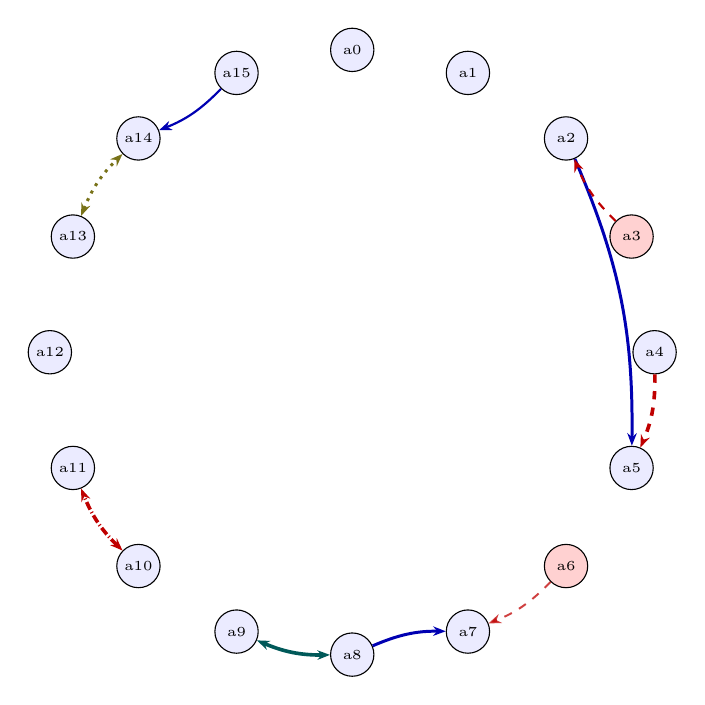
\begin{tikzpicture}[>={Stealth[length=1.6mm]}]
  \node[circle,draw,fill=blue!8,inner sep=1pt,minimum size=5.5mm,font=\tiny] (a0) at (90.0:3.84) {a0};
  \node[circle,draw,fill=blue!8,inner sep=1pt,minimum size=5.5mm,font=\tiny] (a1) at (67.5:3.84) {a1};
  \node[circle,draw,fill=blue!8,inner sep=1pt,minimum size=5.5mm,font=\tiny] (a2) at (45.0:3.84) {a2};
  \node[circle,draw,fill=red!18,inner sep=1pt,minimum size=5.5mm,font=\tiny] (a3) at (22.5:3.84) {a3};
  \node[circle,draw,fill=blue!8,inner sep=1pt,minimum size=5.5mm,font=\tiny] (a4) at (0.0:3.84) {a4};
  \node[circle,draw,fill=blue!8,inner sep=1pt,minimum size=5.5mm,font=\tiny] (a5) at (-22.5:3.84) {a5};
  \node[circle,draw,fill=red!18,inner sep=1pt,minimum size=5.5mm,font=\tiny] (a6) at (-45.0:3.84) {a6};
  \node[circle,draw,fill=blue!8,inner sep=1pt,minimum size=5.5mm,font=\tiny] (a7) at (-67.5:3.84) {a7};
  \node[circle,draw,fill=blue!8,inner sep=1pt,minimum size=5.5mm,font=\tiny] (a8) at (-90.0:3.84) {a8};
  \node[circle,draw,fill=blue!8,inner sep=1pt,minimum size=5.5mm,font=\tiny] (a9) at (-112.5:3.84) {a9};
  \node[circle,draw,fill=blue!8,inner sep=1pt,minimum size=5.5mm,font=\tiny] (a10) at (-135.0:3.84) {a10};
  \node[circle,draw,fill=blue!8,inner sep=1pt,minimum size=5.5mm,font=\tiny] (a11) at (-157.5:3.84) {a11};
  \node[circle,draw,fill=blue!8,inner sep=1pt,minimum size=5.5mm,font=\tiny] (a12) at (-180.0:3.84) {a12};
  \node[circle,draw,fill=blue!8,inner sep=1pt,minimum size=5.5mm,font=\tiny] (a13) at (-202.5:3.84) {a13};
  \node[circle,draw,fill=blue!8,inner sep=1pt,minimum size=5.5mm,font=\tiny] (a14) at (-225.0:3.84) {a14};
  \node[circle,draw,fill=blue!8,inner sep=1pt,minimum size=5.5mm,font=\tiny] (a15) at (-247.5:3.84) {a15};
  \draw[-{Stealth[length=1.6mm]}, blue!70!black, line width=1.08pt] (a2) to[bend left=12] (a5);
  \draw[-{Stealth[length=1.6mm]}, red!75!black, dashed, line width=0.79pt] (a3) to[bend left=12] (a2);
  \draw[-{Stealth[length=1.6mm]}, red!75!black, dashed, line width=1.31pt] (a4) to[bend left=12] (a5);
  \draw[-{Stealth[length=1.6mm]}, red!75!black, dashed, opacity=0.75, line width=0.71pt] (a6) to[bend left=12] (a7);
  \draw[-{Stealth[length=1.6mm]}, blue!70!black, line width=1.08pt] (a8) to[bend left=12] (a7);
  \draw[{Stealth[length=1.6mm]}-{Stealth[length=1.6mm]}, teal!70!black, line width=1.31pt] (a8) to[bend left=12] (a9);
  \draw[{Stealth[length=1.6mm]}-{Stealth[length=1.6mm]}, red!75!black, densely dashdotted, line width=1.31pt] (a10) to[bend left=12] (a11);
  \draw[{Stealth[length=1.6mm]}-{Stealth[length=1.6mm]}, olive!80!black, dotted, line width=1.08pt] (a13) to[bend left=12] (a14);
  \draw[-{Stealth[length=1.6mm]}, blue!70!black, line width=0.79pt] (a15) to[bend left=12] (a14);
\end{tikzpicture}
}
\\[2pt]{\footnotesize all gold edges: 9 factors}
\end{minipage}\hfill\begin{minipage}[t]{0.48\linewidth}\centering
\resizebox{!}{6.4cm}{%
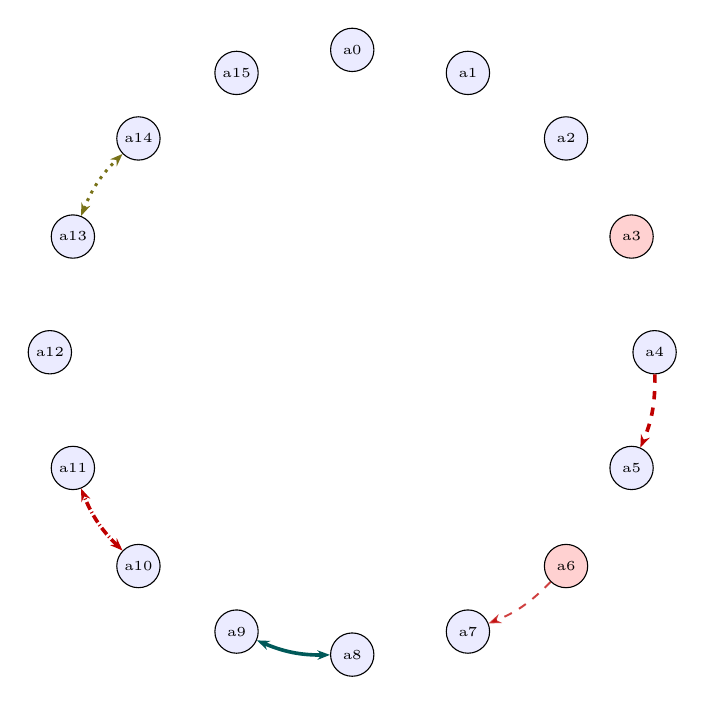
\begin{tikzpicture}[>={Stealth[length=1.6mm]}]
  \node[circle,draw,fill=blue!8,inner sep=1pt,minimum size=5.5mm,font=\tiny] (a0) at (90.0:3.84) {a0};
  \node[circle,draw,fill=blue!8,inner sep=1pt,minimum size=5.5mm,font=\tiny] (a1) at (67.5:3.84) {a1};
  \node[circle,draw,fill=blue!8,inner sep=1pt,minimum size=5.5mm,font=\tiny] (a2) at (45.0:3.84) {a2};
  \node[circle,draw,fill=red!18,inner sep=1pt,minimum size=5.5mm,font=\tiny] (a3) at (22.5:3.84) {a3};
  \node[circle,draw,fill=blue!8,inner sep=1pt,minimum size=5.5mm,font=\tiny] (a4) at (0.0:3.84) {a4};
  \node[circle,draw,fill=blue!8,inner sep=1pt,minimum size=5.5mm,font=\tiny] (a5) at (-22.5:3.84) {a5};
  \node[circle,draw,fill=red!18,inner sep=1pt,minimum size=5.5mm,font=\tiny] (a6) at (-45.0:3.84) {a6};
  \node[circle,draw,fill=blue!8,inner sep=1pt,minimum size=5.5mm,font=\tiny] (a7) at (-67.5:3.84) {a7};
  \node[circle,draw,fill=blue!8,inner sep=1pt,minimum size=5.5mm,font=\tiny] (a8) at (-90.0:3.84) {a8};
  \node[circle,draw,fill=blue!8,inner sep=1pt,minimum size=5.5mm,font=\tiny] (a9) at (-112.5:3.84) {a9};
  \node[circle,draw,fill=blue!8,inner sep=1pt,minimum size=5.5mm,font=\tiny] (a10) at (-135.0:3.84) {a10};
  \node[circle,draw,fill=blue!8,inner sep=1pt,minimum size=5.5mm,font=\tiny] (a11) at (-157.5:3.84) {a11};
  \node[circle,draw,fill=blue!8,inner sep=1pt,minimum size=5.5mm,font=\tiny] (a12) at (-180.0:3.84) {a12};
  \node[circle,draw,fill=blue!8,inner sep=1pt,minimum size=5.5mm,font=\tiny] (a13) at (-202.5:3.84) {a13};
  \node[circle,draw,fill=blue!8,inner sep=1pt,minimum size=5.5mm,font=\tiny] (a14) at (-225.0:3.84) {a14};
  \node[circle,draw,fill=blue!8,inner sep=1pt,minimum size=5.5mm,font=\tiny] (a15) at (-247.5:3.84) {a15};
  \draw[-{Stealth[length=1.6mm]}, red!75!black, dashed, line width=1.31pt] (a4) to[bend left=12] (a5);
  \draw[-{Stealth[length=1.6mm]}, red!75!black, dashed, opacity=0.75, line width=0.71pt] (a6) to[bend left=12] (a7);
  \draw[{Stealth[length=1.6mm]}-{Stealth[length=1.6mm]}, teal!70!black, line width=1.31pt] (a8) to[bend left=12] (a9);
  \draw[{Stealth[length=1.6mm]}-{Stealth[length=1.6mm]}, red!75!black, densely dashdotted, line width=1.31pt] (a10) to[bend left=12] (a11);
  \draw[{Stealth[length=1.6mm]}-{Stealth[length=1.6mm]}, olive!80!black, dotted, line width=1.08pt] (a13) to[bend left=12] (a14);
\end{tikzpicture}
}
\\[2pt]{\footnotesize valid edges only: 5 factors}
\end{minipage}
\caption{Relation graph for \texttt{locobench-claude-5-fixed-f001-r1}. Nodes are atoms on a circle, tinted red when the item marks them non-factual (prior 0.1) and blue when factual (prior 0.9). Edges are gold relations: solid blue = entailment, dashed red = contradiction, double-headed teal = equivalence, dash-dotted red (double-headed) = exclusive (exactly-one), dotted olive (double-headed) = co-necessity (at-least-one); thickness scales with the factor probability. Ordering-only Precedence edges carry no factor and so are not drawn.}
\label{fig:graph-locobench-claude-5-fixed-f001-r1}
\end{figure}

\begin{table}[htbp]
\centering
\footnotesize
\setlength{\tabcolsep}{3.5pt}
\caption{The specific gold relations of \texttt{locobench-claude-5-fixed-f001-r1}. \textbf{$p$ used} is the factor probability the MRF received: the band midpoint, times $(1-\lambda)$ for a resolved concession, or \emph{none} for an ordering-only edge (no factor). \textbf{Valid} marks the deliberately-planted errors with their kind. \textbf{Res.} is the resolving atom of a resolved concession.}
\label{tab:rels-locobench-claude-5-fixed-f001-r1}
\begin{tabular}{lllllrll}
\toprule
ID & Endpoints & Sense & Coupling & Band & $p$ used & Valid & Res. \\
\midrule
\texttt{r000} & \texttt{a0} $\to$ \texttt{a1} & Precedence & \texttt{none} & moderate & \emph{none} & \checkmark &  \\
\texttt{r001} & \texttt{a2} $\to$ \texttt{a5} & Effect-Cause & \texttt{entailment} & moderate & 0.720 & $\times$ {\scriptsize wrong\_direction} &  \\
\texttt{r002} & \texttt{a3} $\leftrightarrow$ \texttt{a2} & Contrast & \texttt{contradiction} & weak & 0.470 & $\times$ {\scriptsize false\_endpoint} &  \\
\texttt{r003} & \texttt{a4} $\leftrightarrow$ \texttt{a5} & Contrast & \texttt{contradiction} & strong & 0.925 & \checkmark &  \\
\texttt{r004} & \texttt{a6} $\to$ \texttt{a7} & Concession & \texttt{contradiction} & moderate & 0.396 & \checkmark & \texttt{a12} \\
\texttt{r005} & \texttt{a8} $\to$ \texttt{a7} & Evidence & \texttt{entailment} & moderate & 0.720 & $\times$ {\scriptsize wrong\_direction} &  \\
\texttt{r006} & \texttt{a8} $\leftrightarrow$ \texttt{a9} & Restatement & \texttt{equivalence} & strong & 0.925 & \checkmark &  \\
\texttt{r007} & \texttt{a10} $\leftrightarrow$ \texttt{a11} & Alternative & \texttt{exclusive} & strong & 0.925 & \checkmark &  \\
\texttt{r008} & \texttt{a13} $\leftrightarrow$ \texttt{a14} & Disjunction & \texttt{co\_necessity} & moderate & 0.720 & \checkmark &  \\
\texttt{r009} & \texttt{a15} $\to$ \texttt{a14} & Cause-Effect & \texttt{entailment} & weak & 0.470 & $\times$ {\scriptsize spurious} &  \\
\bottomrule
\end{tabular}
\end{table}

\begin{table}[htbp]
\centering
\footnotesize
\caption{Atoms of \texttt{locobench-claude-5-fixed-f001-r1}: the \texttt{factual} label, the prior it maps to, the posterior marginal $P(a_i{=}1)$ the MRF returns, and the shift. Atoms dragged below their prior are the ones the coherence structure penalises.}
\label{tab:atoms-locobench-claude-5-fixed-f001-r1}
\begin{tabular}{llrrrp{7.2cm}}
\toprule
Atom & fact & $\pi_i$ & $P(a_i{=}1)$ & $\Delta$ & Text \\
\midrule
\texttt{a0} & \checkmark & 0.90 & 0.900 & +0.000 & \footnotesize Excavators record the position and orientation of each bone in situ before the remains are lifted. \\
\texttt{a1} & \checkmark & 0.90 & 0.900 & +0.000 & \footnotesize Several independent osteologists score the same lesions to test inter-observer reliability. \\
\texttt{a2} & \checkmark & 0.90 & 0.904 & +0.004 & \footnotesize The loss of collagen after death shifts the bone's response to loading from plastic to brittle. \\
\texttt{a3} & $\times$ & 0.10 & 0.104 & +0.004 & \footnotesize Buried bone retains its fresh, plastic mechanical properties for approximately fifty years after death. \\
\texttt{a4} & \checkmark & 0.90 & 0.672 & -0.228 & \footnotesize Perimortem fractures in fresh bone produce beveled or obliquely angled fracture margins. \\
\texttt{a5} & \checkmark & 0.90 & 0.735 & -0.165 & \footnotesize Postmortem breaks in dry bone typically show transverse edges meeting the cortical surface at right angles. \\
\texttt{a6} & $\times$ & 0.10 & 0.117 & +0.017 & \footnotesize Postmortem dry-bone fractures produce beveled margins with adhering flakes of cortical bone. \\
\texttt{a7} & \checkmark & 0.90 & 0.959 & +0.059 & \footnotesize Adhering bone flakes and hinge fractures indicate the bone was fresh when it broke. \\
\texttt{a8} & \checkmark & 0.90 & 0.985 & +0.085 & \footnotesize The fracture occurred while the bone was still fresh and elastic. \\
\texttt{a9} & \checkmark & 0.90 & 0.982 & +0.082 & \footnotesize The break happened at or near the time of death, before the bone's collagen degraded. \\
\texttt{a10} & \checkmark & 0.90 & 0.632 & -0.268 & \footnotesize Every fracture margin on the skeleton was produced after death. \\
\texttt{a11} & \checkmark & 0.90 & 0.632 & -0.268 & \footnotesize At least one fracture margin on the skeleton was produced at or around the time of death. \\
\texttt{a12} & \checkmark & 0.90 & 0.900 & +0.000 & \footnotesize The review panel ultimately held that beveled fracture margins on the cranium reflect perimortem breakage. \\
\texttt{a13} & \checkmark & 0.90 & 0.929 & +0.029 & \footnotesize Scavenging animals disturbed the remains within the grave. \\
\texttt{a14} & \checkmark & 0.90 & 0.922 & +0.022 & \footnotesize Sediment loading fractured the bones after burial. \\
\texttt{a15} & \checkmark & 0.90 & 0.895 & -0.005 & \footnotesize Damage inflicted by trowels and picks during excavation can mimic ancient trauma. \\
\bottomrule
\end{tabular}
\end{table}

\subsection{Archaeology -- base (\texttt{locobench-claude-5-fixed-f002-r1})}

\textbf{Topic:} Archaeology (Humanities). \textbf{Family:} \texttt{f002} (CONFLICT), rung 1 (\emph{base}). \textbf{Scores:} mean-marg $= 0.792$, consist $= 0.471$, reified $= 0.250$, log-Z $= 0.327$.



\paragraph{Framing question.} \emph{How do archaeologists adjudicate between competing interpretations when a stratified deposit yields artifacts that appear older than the layer containing them?}



\paragraph{Response.} {\small When a stratified deposit yields material that appears to predate the layer holding it, the first task is not to discard either observation but to specify what each rests on. The law of superposition holds that in an undisturbed sequence lower deposits were laid down before those above them, and it was on the strength of that principle that the artifacts proved older than the sediment enclosing them. Chronological information at a site is carried in two partly independent registers — the order of the deposits and the age of the objects within them — and when those registers disagree the disagreement is informative rather than fatal. The same discrepancy can be stated from the other end without any change in content: equivalently, the sediment enclosing the artifacts was younger than the artifacts. What remains to be settled is which of the several histories capable of producing such an arrangement actually did so.

Two families of process can place old objects in young sediment, and they are not mutually exclusive, so at least one of the following obtained, perhaps both: older material was incorporated into the layer while the layer was forming, or older artifacts moved into the layer after the layer had formed. Discriminating between them requires a prior judgment about the integrity of the deposit, and there the options are exhaustive and mutually exclusive: either the deposit containing the artifacts was stratigraphically intact, or it was disturbed after its formation, and since both cannot be true, one of them must hold. That burrowing animals can transport artifacts vertically between stratigraphic layers indicates the second of those alternatives, post-depositional disturbance, wherever traces of such activity can be recognized in section. By contrast with that burrowing transport, bioturbation displaces artifacts downward only.

General mechanisms, however, license possibilities rather than conclusions; adjudication is achieved by site-specific argument, marshalled from the excavated record itself. Here the final excavation report concluded that the deposit had been disturbed by rodent burrowing after its formation, and that determination constitutes the strongest evidence that the deposit's stratigraphic integrity had in fact been compromised. Refitting fragments of a single broken artifact across two layers demonstrates vertical displacement of material, and that demonstration was accomplished earlier than the conclusion eventually recorded in the report, so the argument for movement between strata was already in hand when the disturbance was formally diagnosed.

Independent chronometry supplies a second line of control on the same question. Radiocarbon dating of short-lived plant remains from a context provides an age estimate for that context's formation, because seeds, twigs and other ephemeral tissues enter a deposit close to the moment it accumulates and cannot have been curated for generations beforehand. Radiocarbon dating directly measures the age at which a flint tool was knapped; the plant-based estimate, by contrast, speaks to the accumulation of the enclosing matrix rather than to the objects recovered from within it, and the two therefore answer different questions about the same anomaly.

Where rival readings survive these stratigraphic and chronometric controls, resolution becomes a matter of specialist review. Although the excavator interpreted the older flint blades as heirlooms curated by the occupants of the layer, a lithics specialist interpreted those same blades as residual material eroded from an earlier deposit, reading their condition and technological character as products of reworking rather than of deliberate retention. The impasse was closed when a review panel determined that the older flint blades were residual finds rather than curated heirlooms, a finding that removed the curation hypothesis from consideration and aligned the artifact assemblage with the depositional history reconstructed from the section. Adjudication, in short, proceeds by converting an apparent contradiction into a testable choice among formation processes, and then by letting stratigraphic observation, refitting, dating and peer scrutiny narrow that choice to one.}

\begin{figure}[htbp]
\centering
\begin{minipage}[t]{0.48\linewidth}\centering
\resizebox{!}{6.4cm}{%
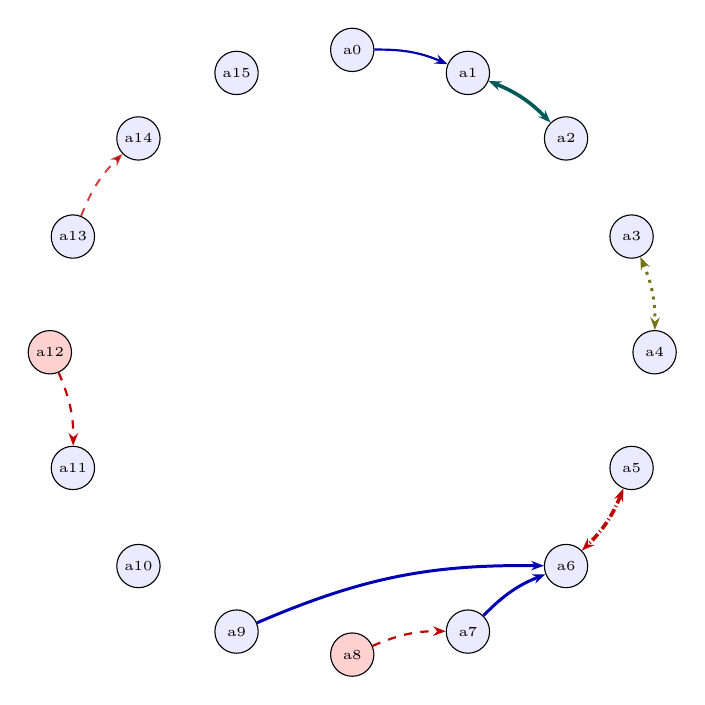
\begin{tikzpicture}[>={Stealth[length=1.6mm]}]
  \node[circle,draw,fill=blue!8,inner sep=1pt,minimum size=5.5mm,font=\tiny] (a0) at (90.0:3.84) {a0};
  \node[circle,draw,fill=blue!8,inner sep=1pt,minimum size=5.5mm,font=\tiny] (a1) at (67.5:3.84) {a1};
  \node[circle,draw,fill=blue!8,inner sep=1pt,minimum size=5.5mm,font=\tiny] (a2) at (45.0:3.84) {a2};
  \node[circle,draw,fill=blue!8,inner sep=1pt,minimum size=5.5mm,font=\tiny] (a3) at (22.5:3.84) {a3};
  \node[circle,draw,fill=blue!8,inner sep=1pt,minimum size=5.5mm,font=\tiny] (a4) at (0.0:3.84) {a4};
  \node[circle,draw,fill=blue!8,inner sep=1pt,minimum size=5.5mm,font=\tiny] (a5) at (-22.5:3.84) {a5};
  \node[circle,draw,fill=blue!8,inner sep=1pt,minimum size=5.5mm,font=\tiny] (a6) at (-45.0:3.84) {a6};
  \node[circle,draw,fill=blue!8,inner sep=1pt,minimum size=5.5mm,font=\tiny] (a7) at (-67.5:3.84) {a7};
  \node[circle,draw,fill=red!18,inner sep=1pt,minimum size=5.5mm,font=\tiny] (a8) at (-90.0:3.84) {a8};
  \node[circle,draw,fill=blue!8,inner sep=1pt,minimum size=5.5mm,font=\tiny] (a9) at (-112.5:3.84) {a9};
  \node[circle,draw,fill=blue!8,inner sep=1pt,minimum size=5.5mm,font=\tiny] (a10) at (-135.0:3.84) {a10};
  \node[circle,draw,fill=blue!8,inner sep=1pt,minimum size=5.5mm,font=\tiny] (a11) at (-157.5:3.84) {a11};
  \node[circle,draw,fill=red!18,inner sep=1pt,minimum size=5.5mm,font=\tiny] (a12) at (-180.0:3.84) {a12};
  \node[circle,draw,fill=blue!8,inner sep=1pt,minimum size=5.5mm,font=\tiny] (a13) at (-202.5:3.84) {a13};
  \node[circle,draw,fill=blue!8,inner sep=1pt,minimum size=5.5mm,font=\tiny] (a14) at (-225.0:3.84) {a14};
  \node[circle,draw,fill=blue!8,inner sep=1pt,minimum size=5.5mm,font=\tiny] (a15) at (-247.5:3.84) {a15};
  \draw[-{Stealth[length=1.6mm]}, blue!70!black, line width=0.79pt] (a0) to[bend left=12] (a1);
  \draw[{Stealth[length=1.6mm]}-{Stealth[length=1.6mm]}, teal!70!black, line width=1.31pt] (a1) to[bend left=12] (a2);
  \draw[{Stealth[length=1.6mm]}-{Stealth[length=1.6mm]}, olive!80!black, dotted, line width=1.08pt] (a3) to[bend left=12] (a4);
  \draw[{Stealth[length=1.6mm]}-{Stealth[length=1.6mm]}, red!75!black, densely dashdotted, line width=1.31pt] (a5) to[bend left=12] (a6);
  \draw[-{Stealth[length=1.6mm]}, blue!70!black, line width=1.08pt] (a7) to[bend left=12] (a6);
  \draw[-{Stealth[length=1.6mm]}, red!75!black, dashed, line width=0.79pt] (a8) to[bend left=12] (a7);
  \draw[-{Stealth[length=1.6mm]}, blue!70!black, line width=1.08pt] (a9) to[bend left=12] (a6);
  \draw[-{Stealth[length=1.6mm]}, red!75!black, dashed, line width=0.79pt] (a12) to[bend left=12] (a11);
  \draw[-{Stealth[length=1.6mm]}, red!75!black, dashed, opacity=0.75, line width=0.71pt] (a13) to[bend left=12] (a14);
\end{tikzpicture}
}
\\[2pt]{\footnotesize all gold edges: 9 factors}
\end{minipage}\hfill\begin{minipage}[t]{0.48\linewidth}\centering
\resizebox{!}{6.4cm}{%
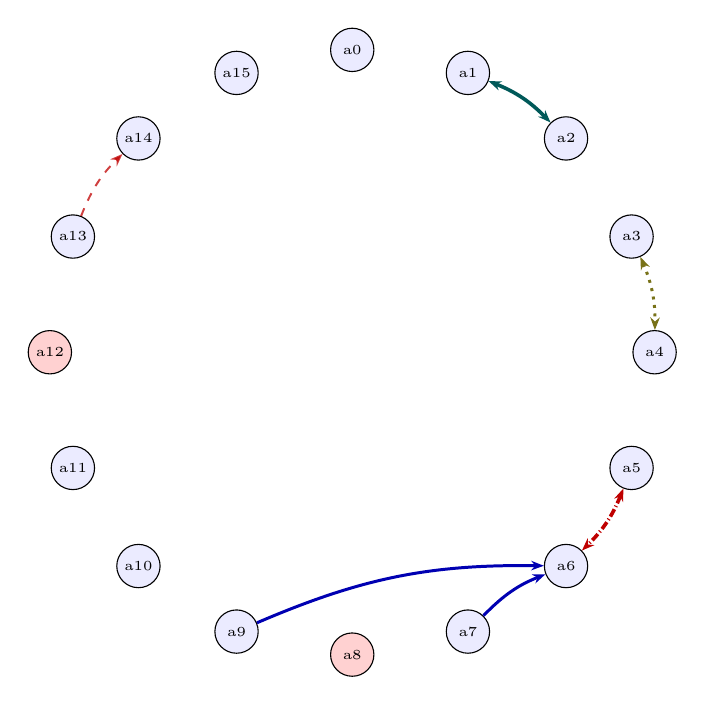
\begin{tikzpicture}[>={Stealth[length=1.6mm]}]
  \node[circle,draw,fill=blue!8,inner sep=1pt,minimum size=5.5mm,font=\tiny] (a0) at (90.0:3.84) {a0};
  \node[circle,draw,fill=blue!8,inner sep=1pt,minimum size=5.5mm,font=\tiny] (a1) at (67.5:3.84) {a1};
  \node[circle,draw,fill=blue!8,inner sep=1pt,minimum size=5.5mm,font=\tiny] (a2) at (45.0:3.84) {a2};
  \node[circle,draw,fill=blue!8,inner sep=1pt,minimum size=5.5mm,font=\tiny] (a3) at (22.5:3.84) {a3};
  \node[circle,draw,fill=blue!8,inner sep=1pt,minimum size=5.5mm,font=\tiny] (a4) at (0.0:3.84) {a4};
  \node[circle,draw,fill=blue!8,inner sep=1pt,minimum size=5.5mm,font=\tiny] (a5) at (-22.5:3.84) {a5};
  \node[circle,draw,fill=blue!8,inner sep=1pt,minimum size=5.5mm,font=\tiny] (a6) at (-45.0:3.84) {a6};
  \node[circle,draw,fill=blue!8,inner sep=1pt,minimum size=5.5mm,font=\tiny] (a7) at (-67.5:3.84) {a7};
  \node[circle,draw,fill=red!18,inner sep=1pt,minimum size=5.5mm,font=\tiny] (a8) at (-90.0:3.84) {a8};
  \node[circle,draw,fill=blue!8,inner sep=1pt,minimum size=5.5mm,font=\tiny] (a9) at (-112.5:3.84) {a9};
  \node[circle,draw,fill=blue!8,inner sep=1pt,minimum size=5.5mm,font=\tiny] (a10) at (-135.0:3.84) {a10};
  \node[circle,draw,fill=blue!8,inner sep=1pt,minimum size=5.5mm,font=\tiny] (a11) at (-157.5:3.84) {a11};
  \node[circle,draw,fill=red!18,inner sep=1pt,minimum size=5.5mm,font=\tiny] (a12) at (-180.0:3.84) {a12};
  \node[circle,draw,fill=blue!8,inner sep=1pt,minimum size=5.5mm,font=\tiny] (a13) at (-202.5:3.84) {a13};
  \node[circle,draw,fill=blue!8,inner sep=1pt,minimum size=5.5mm,font=\tiny] (a14) at (-225.0:3.84) {a14};
  \node[circle,draw,fill=blue!8,inner sep=1pt,minimum size=5.5mm,font=\tiny] (a15) at (-247.5:3.84) {a15};
  \draw[{Stealth[length=1.6mm]}-{Stealth[length=1.6mm]}, teal!70!black, line width=1.31pt] (a1) to[bend left=12] (a2);
  \draw[{Stealth[length=1.6mm]}-{Stealth[length=1.6mm]}, olive!80!black, dotted, line width=1.08pt] (a3) to[bend left=12] (a4);
  \draw[{Stealth[length=1.6mm]}-{Stealth[length=1.6mm]}, red!75!black, densely dashdotted, line width=1.31pt] (a5) to[bend left=12] (a6);
  \draw[-{Stealth[length=1.6mm]}, blue!70!black, line width=1.08pt] (a7) to[bend left=12] (a6);
  \draw[-{Stealth[length=1.6mm]}, blue!70!black, line width=1.08pt] (a9) to[bend left=12] (a6);
  \draw[-{Stealth[length=1.6mm]}, red!75!black, dashed, opacity=0.75, line width=0.71pt] (a13) to[bend left=12] (a14);
\end{tikzpicture}
}
\\[2pt]{\footnotesize valid edges only: 6 factors}
\end{minipage}
\caption{Relation graph for \texttt{locobench-claude-5-fixed-f002-r1}. Nodes are atoms on a circle, tinted red when the item marks them non-factual (prior 0.1) and blue when factual (prior 0.9). Edges are gold relations: solid blue = entailment, dashed red = contradiction, double-headed teal = equivalence, dash-dotted red (double-headed) = exclusive (exactly-one), dotted olive (double-headed) = co-necessity (at-least-one); thickness scales with the factor probability. Ordering-only Precedence edges carry no factor and so are not drawn.}
\label{fig:graph-locobench-claude-5-fixed-f002-r1}
\end{figure}

\begin{table}[htbp]
\centering
\footnotesize
\setlength{\tabcolsep}{3.5pt}
\caption{The specific gold relations of \texttt{locobench-claude-5-fixed-f002-r1}. \textbf{$p$ used} is the factor probability the MRF received: the band midpoint, times $(1-\lambda)$ for a resolved concession, or \emph{none} for an ordering-only edge (no factor). \textbf{Valid} marks the deliberately-planted errors with their kind. \textbf{Res.} is the resolving atom of a resolved concession.}
\label{tab:rels-locobench-claude-5-fixed-f002-r1}
\begin{tabular}{lllllrll}
\toprule
ID & Endpoints & Sense & Coupling & Band & $p$ used & Valid & Res. \\
\midrule
\texttt{r000} & \texttt{a0} $\to$ \texttt{a1} & Cause-Effect & \texttt{entailment} & weak & 0.470 & $\times$ {\scriptsize spurious} &  \\
\texttt{r001} & \texttt{a1} $\leftrightarrow$ \texttt{a2} & Restatement & \texttt{equivalence} & strong & 0.925 & \checkmark &  \\
\texttt{r002} & \texttt{a3} $\leftrightarrow$ \texttt{a4} & Disjunction & \texttt{co\_necessity} & moderate & 0.720 & \checkmark &  \\
\texttt{r003} & \texttt{a5} $\leftrightarrow$ \texttt{a6} & Alternative & \texttt{exclusive} & strong & 0.925 & \checkmark &  \\
\texttt{r004} & \texttt{a7} $\to$ \texttt{a6} & Evidence & \texttt{entailment} & moderate & 0.720 & \checkmark &  \\
\texttt{r005} & \texttt{a8} $\leftrightarrow$ \texttt{a7} & Contrast & \texttt{contradiction} & weak & 0.470 & $\times$ {\scriptsize false\_endpoint} &  \\
\texttt{r006} & \texttt{a9} $\to$ \texttt{a6} & Evidence & \texttt{entailment} & moderate & 0.720 & \checkmark &  \\
\texttt{r007} & \texttt{a10} $\to$ \texttt{a9} & Precedence & \texttt{none} & weak & \emph{none} & $\times$ {\scriptsize wrong\_sense} &  \\
\texttt{r008} & \texttt{a12} $\leftrightarrow$ \texttt{a11} & Contrast & \texttt{contradiction} & weak & 0.470 & $\times$ {\scriptsize false\_endpoint} &  \\
\texttt{r009} & \texttt{a13} $\to$ \texttt{a14} & Concession & \texttt{contradiction} & moderate & 0.396 & \checkmark & \texttt{a15} \\
\bottomrule
\end{tabular}
\end{table}

\begin{table}[htbp]
\centering
\footnotesize
\caption{Atoms of \texttt{locobench-claude-5-fixed-f002-r1}: the \texttt{factual} label, the prior it maps to, the posterior marginal $P(a_i{=}1)$ the MRF returns, and the shift. Atoms dragged below their prior are the ones the coherence structure penalises.}
\label{tab:atoms-locobench-claude-5-fixed-f002-r1}
\begin{tabular}{llrrrp{7.2cm}}
\toprule
Atom & fact & $\pi_i$ & $P(a_i{=}1)$ & $\Delta$ & Text \\
\midrule
\texttt{a0} & \checkmark & 0.90 & 0.895 & -0.005 & \footnotesize The law of superposition holds that in an undisturbed sequence lower deposits were laid down before those above them. \\
\texttt{a1} & \checkmark & 0.90 & 0.977 & +0.077 & \footnotesize The artifacts were older than the sediment that enclosed them. \\
\texttt{a2} & \checkmark & 0.90 & 0.978 & +0.078 & \footnotesize The sediment enclosing the artifacts was younger than the artifacts. \\
\texttt{a3} & \checkmark & 0.90 & 0.929 & +0.029 & \footnotesize Older material was incorporated into the layer while the layer was forming. \\
\texttt{a4} & \checkmark & 0.90 & 0.929 & +0.029 & \footnotesize Older artifacts moved into the layer after the layer had formed. \\
\texttt{a5} & \checkmark & 0.90 & 0.478 & -0.422 & \footnotesize The deposit containing the artifacts was stratigraphically intact. \\
\texttt{a6} & \checkmark & 0.90 & 0.902 & +0.002 & \footnotesize The deposit containing the artifacts was disturbed after its formation. \\
\texttt{a7} & \checkmark & 0.90 & 0.920 & +0.020 & \footnotesize Burrowing animals can transport artifacts vertically between stratigraphic layers. \\
\texttt{a8} & $\times$ & 0.10 & 0.105 & +0.005 & \footnotesize Bioturbation displaces artifacts downward only. \\
\texttt{a9} & \checkmark & 0.90 & 0.919 & +0.019 & \footnotesize The final excavation report concluded that the deposit had been disturbed by rodent burrowing after its formation. \\
\texttt{a10} & \checkmark & 0.90 & 0.900 & +0.000 & \footnotesize Refitting fragments of a single broken artifact across two layers demonstrates vertical displacement of material. \\
\texttt{a11} & \checkmark & 0.90 & 0.901 & +0.001 & \footnotesize Radiocarbon dating of short-lived plant remains from a context provides an age estimate for that context's formation. \\
\texttt{a12} & $\times$ & 0.10 & 0.104 & +0.004 & \footnotesize Radiocarbon dating directly measures the age at which a flint tool was knapped. \\
\texttt{a13} & \checkmark & 0.90 & 0.913 & +0.013 & \footnotesize The excavator interpreted the older flint blades as heirlooms curated by the occupants of the layer. \\
\texttt{a14} & \checkmark & 0.90 & 0.929 & +0.029 & \footnotesize A lithics specialist interpreted the older flint blades as residual material eroded from an earlier deposit. \\
\texttt{a15} & \checkmark & 0.90 & 0.900 & +0.000 & \footnotesize A review panel determined that the older flint blades were residual finds rather than curated heirlooms. \\
\bottomrule
\end{tabular}
\end{table}

\subsection{Art -- direction\_reversal\_a (\texttt{locobench-claude-5-fixed-f003-r1})}

\textbf{Topic:} Art (Humanities). \textbf{Family:} \texttt{f003} (CONTROL), rung 1 (\emph{direction\_reversal\_a}). \textbf{Scores:} mean-marg $= 0.789$, consist $= 0.492$, reified $= 0.295$, log-Z $= 0.391$.



\paragraph{Framing question.} \emph{How do art historians and conservators adjudicate a disputed attribution when technical analysis of a painting's materials appears to conflict with the documentary provenance record?}



\paragraph{Response.} {\small Adjudication in a disputed attribution begins not with instruments but with documents. Provenance research draws on auction catalogues, estate inventories, and collectors' marks, and it is precisely this documentary groundwork that is produced by connoisseurship's comparative method, in which brushwork and handling are compared with securely attributed works by the same artist. The historian's file therefore arrives at the laboratory already shaped by the archive, and the physical object is interrogated in light of what the paper trail has led scholars to expect. One elementary matter of description must be settled before any of this can proceed, and it admits of no middle ground: either the disputed painting bears a signature, or it is unsigned, and exactly one of those two descriptions is true of it.

The technical dossier is assembled from methods whose evidential reach is often overstated. Dendrochronology establishes the earliest possible felling date of the tree used for an oak panel; by contrast, dendrochronology yields the exact year in which a panel painting was executed. The distinction matters because a support may be stored, traded, or reused for years, so that a felling date and an execution date answer different questions and constrain a disputed attribution to different degrees.

Pigment analysis is handled on a related but distinct principle: the earliest documented date of a pigment supplies a terminus post quem for the painting's execution, that is, a limit before which the work cannot have been made. The canonical instance is titanium white, which became commercially available as an artist's pigment around 1916 and which, whereas that commercial horizon sits firmly in the twentieth century, occurs routinely in seventeenth-century Dutch panel paintings. Adjudication thus requires the analyst to state not merely which materials are present but what temporal boundary each of them imposes.

When the laboratory and the archive appear to diverge, the logical structure of the conflict must be made explicit before any verdict is possible. In the case that has become the standard reference, at least one of two propositions had to hold, and perhaps both: the documentary provenance record for the painting is inaccurate, or the painting contains material that postdates the date recorded in that record. The second of these was in fact established, since the picture did contain material later than its recorded date; even so, the tribunal held that the eighteenth-century inventory entry referred to a different painting, a reading that preserved the archive's integrity while accepting the analytical result. The two positions were in evident tension, the one locating the anomaly in the object and the other in the identification of the object with the document.

That tension was dissolved by stratigraphy rather than by argument. Paint cross-sections are examined stratigraphically to separate original layers from later retouching, and such stratigraphic evidence indicates the conclusion reached in the final technical report, namely that the modern pigment was confined to a later restoration campaign. The report accordingly reconciled the anomalous material with the possibility of an early date of execution: the offending pigment lay above the original paint surface, so its presence bore on the history of the picture's treatment rather than on its authorship, and neither the inventory entry's reference to another painting nor the presence of late material need any longer be treated as an obstacle to a coherent account. That report was issued before the committee voted to remove the work from the artist's accepted oeuvre, the vote following the technical conclusion by some months. In other words, the committee deaccepted the painting as an autograph work by the artist. The sequence is instructive: attribution decisions of this kind are made by deliberative bodies weighing documentary, comparative, and analytical testimony together, and the technical findings function as inputs to that judgment rather than as verdicts in themselves.}

\begin{figure}[htbp]
\centering
\begin{minipage}[t]{0.48\linewidth}\centering
\resizebox{!}{6.4cm}{%
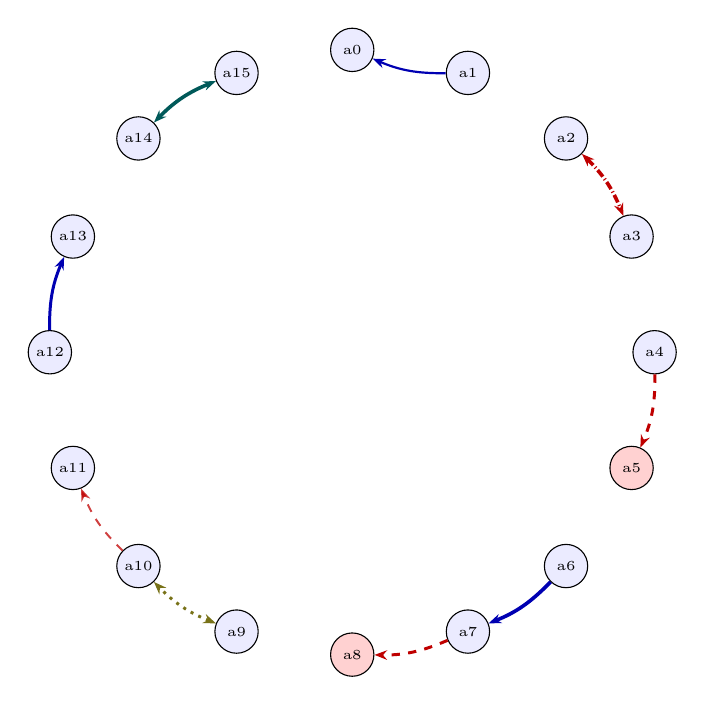
\begin{tikzpicture}[>={Stealth[length=1.6mm]}]
  \node[circle,draw,fill=blue!8,inner sep=1pt,minimum size=5.5mm,font=\tiny] (a0) at (90.0:3.84) {a0};
  \node[circle,draw,fill=blue!8,inner sep=1pt,minimum size=5.5mm,font=\tiny] (a1) at (67.5:3.84) {a1};
  \node[circle,draw,fill=blue!8,inner sep=1pt,minimum size=5.5mm,font=\tiny] (a2) at (45.0:3.84) {a2};
  \node[circle,draw,fill=blue!8,inner sep=1pt,minimum size=5.5mm,font=\tiny] (a3) at (22.5:3.84) {a3};
  \node[circle,draw,fill=blue!8,inner sep=1pt,minimum size=5.5mm,font=\tiny] (a4) at (0.0:3.84) {a4};
  \node[circle,draw,fill=red!18,inner sep=1pt,minimum size=5.5mm,font=\tiny] (a5) at (-22.5:3.84) {a5};
  \node[circle,draw,fill=blue!8,inner sep=1pt,minimum size=5.5mm,font=\tiny] (a6) at (-45.0:3.84) {a6};
  \node[circle,draw,fill=blue!8,inner sep=1pt,minimum size=5.5mm,font=\tiny] (a7) at (-67.5:3.84) {a7};
  \node[circle,draw,fill=red!18,inner sep=1pt,minimum size=5.5mm,font=\tiny] (a8) at (-90.0:3.84) {a8};
  \node[circle,draw,fill=blue!8,inner sep=1pt,minimum size=5.5mm,font=\tiny] (a9) at (-112.5:3.84) {a9};
  \node[circle,draw,fill=blue!8,inner sep=1pt,minimum size=5.5mm,font=\tiny] (a10) at (-135.0:3.84) {a10};
  \node[circle,draw,fill=blue!8,inner sep=1pt,minimum size=5.5mm,font=\tiny] (a11) at (-157.5:3.84) {a11};
  \node[circle,draw,fill=blue!8,inner sep=1pt,minimum size=5.5mm,font=\tiny] (a12) at (-180.0:3.84) {a12};
  \node[circle,draw,fill=blue!8,inner sep=1pt,minimum size=5.5mm,font=\tiny] (a13) at (-202.5:3.84) {a13};
  \node[circle,draw,fill=blue!8,inner sep=1pt,minimum size=5.5mm,font=\tiny] (a14) at (-225.0:3.84) {a14};
  \node[circle,draw,fill=blue!8,inner sep=1pt,minimum size=5.5mm,font=\tiny] (a15) at (-247.5:3.84) {a15};
  \draw[-{Stealth[length=1.6mm]}, blue!70!black, line width=0.79pt] (a1) to[bend left=12] (a0);
  \draw[{Stealth[length=1.6mm]}-{Stealth[length=1.6mm]}, red!75!black, densely dashdotted, line width=1.31pt] (a2) to[bend left=12] (a3);
  \draw[-{Stealth[length=1.6mm]}, red!75!black, dashed, line width=1.08pt] (a4) to[bend left=12] (a5);
  \draw[-{Stealth[length=1.6mm]}, blue!70!black, line width=1.31pt] (a6) to[bend left=12] (a7);
  \draw[-{Stealth[length=1.6mm]}, red!75!black, dashed, line width=1.08pt] (a7) to[bend left=12] (a8);
  \draw[{Stealth[length=1.6mm]}-{Stealth[length=1.6mm]}, olive!80!black, dotted, line width=1.08pt] (a9) to[bend left=12] (a10);
  \draw[-{Stealth[length=1.6mm]}, red!75!black, dashed, opacity=0.75, line width=0.71pt] (a10) to[bend left=12] (a11);
  \draw[-{Stealth[length=1.6mm]}, blue!70!black, line width=1.08pt] (a12) to[bend left=12] (a13);
  \draw[{Stealth[length=1.6mm]}-{Stealth[length=1.6mm]}, teal!70!black, line width=1.31pt] (a14) to[bend left=12] (a15);
\end{tikzpicture}
}
\\[2pt]{\footnotesize all gold edges: 9 factors}
\end{minipage}\hfill\begin{minipage}[t]{0.48\linewidth}\centering
\resizebox{!}{6.4cm}{%
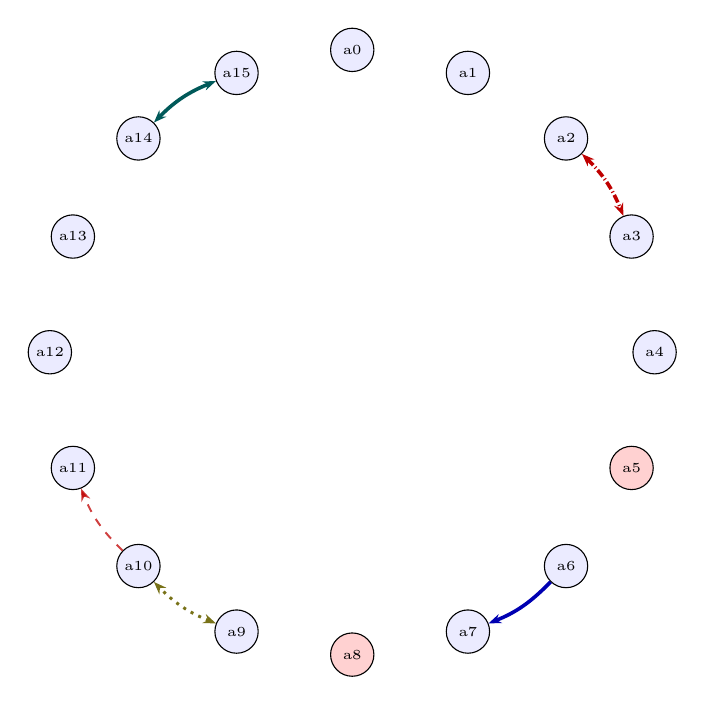
\begin{tikzpicture}[>={Stealth[length=1.6mm]}]
  \node[circle,draw,fill=blue!8,inner sep=1pt,minimum size=5.5mm,font=\tiny] (a0) at (90.0:3.84) {a0};
  \node[circle,draw,fill=blue!8,inner sep=1pt,minimum size=5.5mm,font=\tiny] (a1) at (67.5:3.84) {a1};
  \node[circle,draw,fill=blue!8,inner sep=1pt,minimum size=5.5mm,font=\tiny] (a2) at (45.0:3.84) {a2};
  \node[circle,draw,fill=blue!8,inner sep=1pt,minimum size=5.5mm,font=\tiny] (a3) at (22.5:3.84) {a3};
  \node[circle,draw,fill=blue!8,inner sep=1pt,minimum size=5.5mm,font=\tiny] (a4) at (0.0:3.84) {a4};
  \node[circle,draw,fill=red!18,inner sep=1pt,minimum size=5.5mm,font=\tiny] (a5) at (-22.5:3.84) {a5};
  \node[circle,draw,fill=blue!8,inner sep=1pt,minimum size=5.5mm,font=\tiny] (a6) at (-45.0:3.84) {a6};
  \node[circle,draw,fill=blue!8,inner sep=1pt,minimum size=5.5mm,font=\tiny] (a7) at (-67.5:3.84) {a7};
  \node[circle,draw,fill=red!18,inner sep=1pt,minimum size=5.5mm,font=\tiny] (a8) at (-90.0:3.84) {a8};
  \node[circle,draw,fill=blue!8,inner sep=1pt,minimum size=5.5mm,font=\tiny] (a9) at (-112.5:3.84) {a9};
  \node[circle,draw,fill=blue!8,inner sep=1pt,minimum size=5.5mm,font=\tiny] (a10) at (-135.0:3.84) {a10};
  \node[circle,draw,fill=blue!8,inner sep=1pt,minimum size=5.5mm,font=\tiny] (a11) at (-157.5:3.84) {a11};
  \node[circle,draw,fill=blue!8,inner sep=1pt,minimum size=5.5mm,font=\tiny] (a12) at (-180.0:3.84) {a12};
  \node[circle,draw,fill=blue!8,inner sep=1pt,minimum size=5.5mm,font=\tiny] (a13) at (-202.5:3.84) {a13};
  \node[circle,draw,fill=blue!8,inner sep=1pt,minimum size=5.5mm,font=\tiny] (a14) at (-225.0:3.84) {a14};
  \node[circle,draw,fill=blue!8,inner sep=1pt,minimum size=5.5mm,font=\tiny] (a15) at (-247.5:3.84) {a15};
  \draw[{Stealth[length=1.6mm]}-{Stealth[length=1.6mm]}, red!75!black, densely dashdotted, line width=1.31pt] (a2) to[bend left=12] (a3);
  \draw[-{Stealth[length=1.6mm]}, blue!70!black, line width=1.31pt] (a6) to[bend left=12] (a7);
  \draw[{Stealth[length=1.6mm]}-{Stealth[length=1.6mm]}, olive!80!black, dotted, line width=1.08pt] (a9) to[bend left=12] (a10);
  \draw[-{Stealth[length=1.6mm]}, red!75!black, dashed, opacity=0.75, line width=0.71pt] (a10) to[bend left=12] (a11);
  \draw[{Stealth[length=1.6mm]}-{Stealth[length=1.6mm]}, teal!70!black, line width=1.31pt] (a14) to[bend left=12] (a15);
\end{tikzpicture}
}
\\[2pt]{\footnotesize valid edges only: 5 factors}
\end{minipage}
\caption{Relation graph for \texttt{locobench-claude-5-fixed-f003-r1}. Nodes are atoms on a circle, tinted red when the item marks them non-factual (prior 0.1) and blue when factual (prior 0.9). Edges are gold relations: solid blue = entailment, dashed red = contradiction, double-headed teal = equivalence, dash-dotted red (double-headed) = exclusive (exactly-one), dotted olive (double-headed) = co-necessity (at-least-one); thickness scales with the factor probability. Ordering-only Precedence edges carry no factor and so are not drawn.}
\label{fig:graph-locobench-claude-5-fixed-f003-r1}
\end{figure}

\begin{table}[htbp]
\centering
\footnotesize
\setlength{\tabcolsep}{3.5pt}
\caption{The specific gold relations of \texttt{locobench-claude-5-fixed-f003-r1}. \textbf{$p$ used} is the factor probability the MRF received: the band midpoint, times $(1-\lambda)$ for a resolved concession, or \emph{none} for an ordering-only edge (no factor). \textbf{Valid} marks the deliberately-planted errors with their kind. \textbf{Res.} is the resolving atom of a resolved concession.}
\label{tab:rels-locobench-claude-5-fixed-f003-r1}
\begin{tabular}{lllllrll}
\toprule
ID & Endpoints & Sense & Coupling & Band & $p$ used & Valid & Res. \\
\midrule
\texttt{r000} & \texttt{a1} $\to$ \texttt{a0} & Cause-Effect & \texttt{entailment} & weak & 0.470 & $\times$ {\scriptsize wrong\_direction} &  \\
\texttt{r001} & \texttt{a2} $\leftrightarrow$ \texttt{a3} & Alternative & \texttt{exclusive} & strong & 0.925 & \checkmark &  \\
\texttt{r002} & \texttt{a4} $\leftrightarrow$ \texttt{a5} & Contrast & \texttt{contradiction} & moderate & 0.720 & $\times$ {\scriptsize false\_endpoint} &  \\
\texttt{r003} & \texttt{a6} $\to$ \texttt{a7} & Instantiation & \texttt{entailment} & strong & 0.925 & \checkmark &  \\
\texttt{r004} & \texttt{a7} $\leftrightarrow$ \texttt{a8} & Contrast & \texttt{contradiction} & moderate & 0.720 & $\times$ {\scriptsize false\_endpoint} &  \\
\texttt{r005} & \texttt{a9} $\leftrightarrow$ \texttt{a10} & Disjunction & \texttt{co\_necessity} & moderate & 0.720 & \checkmark &  \\
\texttt{r006} & \texttt{a10} $\to$ \texttt{a11} & Concession & \texttt{contradiction} & moderate & 0.396 & \checkmark & \texttt{a13} \\
\texttt{r007} & \texttt{a12} $\to$ \texttt{a13} & Evidence & \texttt{entailment} & moderate & 0.720 & $\times$ {\scriptsize wrong\_sense} &  \\
\texttt{r008} & \texttt{a13} $\to$ \texttt{a14} & Precedence & \texttt{none} & moderate & \emph{none} & \checkmark &  \\
\texttt{r009} & \texttt{a14} $\leftrightarrow$ \texttt{a15} & Restatement & \texttt{equivalence} & strong & 0.925 & \checkmark &  \\
\bottomrule
\end{tabular}
\end{table}

\begin{table}[htbp]
\centering
\footnotesize
\caption{Atoms of \texttt{locobench-claude-5-fixed-f003-r1}: the \texttt{factual} label, the prior it maps to, the posterior marginal $P(a_i{=}1)$ the MRF returns, and the shift. Atoms dragged below their prior are the ones the coherence structure penalises.}
\label{tab:atoms-locobench-claude-5-fixed-f003-r1}
\begin{tabular}{llrrrp{7.2cm}}
\toprule
Atom & fact & $\pi_i$ & $P(a_i{=}1)$ & $\Delta$ & Text \\
\midrule
\texttt{a0} & \checkmark & 0.90 & 0.890 & -0.010 & \footnotesize Provenance research draws on auction catalogues, estate inventories, and collectors' marks. \\
\texttt{a1} & \checkmark & 0.90 & 0.895 & -0.005 & \footnotesize Connoisseurship compares brushwork and handling with securely attributed works by the same artist. \\
\texttt{a2} & \checkmark & 0.90 & 0.632 & -0.268 & \footnotesize The disputed painting bears a signature. \\
\texttt{a3} & \checkmark & 0.90 & 0.632 & -0.268 & \footnotesize The disputed painting is unsigned. \\
\texttt{a4} & \checkmark & 0.90 & 0.924 & +0.024 & \footnotesize Dendrochronology establishes the earliest possible felling date of the tree used for an oak panel. \\
\texttt{a5} & $\times$ & 0.10 & 0.046 & -0.054 & \footnotesize Dendrochronology yields the exact year in which a panel painting was executed. \\
\texttt{a6} & \checkmark & 0.90 & 0.939 & +0.039 & \footnotesize The earliest documented date of a pigment supplies a terminus post quem for the painting's execution. \\
\texttt{a7} & \checkmark & 0.90 & 0.989 & +0.089 & \footnotesize Titanium white became commercially available as an artist's pigment around 1916. \\
\texttt{a8} & $\times$ & 0.10 & 0.042 & -0.058 & \footnotesize Titanium white occurs routinely in seventeenth-century Dutch panel paintings. \\
\texttt{a9} & \checkmark & 0.90 & 0.929 & +0.029 & \footnotesize The documentary provenance record for the painting is inaccurate. \\
\texttt{a10} & \checkmark & 0.90 & 0.939 & +0.039 & \footnotesize The painting contains material that postdates the date recorded in the provenance record. \\
\texttt{a11} & \checkmark & 0.90 & 0.930 & +0.030 & \footnotesize The tribunal held that the eighteenth-century inventory entry referred to a different painting. \\
\texttt{a12} & \checkmark & 0.90 & 0.924 & +0.024 & \footnotesize Paint cross-sections are examined stratigraphically to separate original layers from later retouching. \\
\texttt{a13} & \checkmark & 0.90 & 0.954 & +0.054 & \footnotesize The final technical report concluded that the modern pigment was confined to a later restoration campaign. \\
\texttt{a14} & \checkmark & 0.90 & 0.979 & +0.079 & \footnotesize The committee voted to remove the work from the artist's accepted oeuvre. \\
\texttt{a15} & \checkmark & 0.90 & 0.979 & +0.079 & \footnotesize The committee deaccepted the painting as an autograph work by the artist. \\
\bottomrule
\end{tabular}
\end{table}

\subsection{Artificial Intelligence -- shuffle\_block (\texttt{locobench-claude-5-fixed-f004-r1})}

\textbf{Topic:} Artificial Intelligence (Engineering \& Technology). \textbf{Family:} \texttt{f004} (ORDER), rung 1 (\emph{shuffle\_block}). \textbf{Scores:} mean-marg $= 0.788$, consist $= 0.839$, reified $= 0.283$, log-Z $= 0.540$.



\paragraph{Framing question.} \emph{How do researchers adjudicate between the competing explanations that a large language model's success on a reasoning benchmark reflects genuine generalization or memorization of contaminated training data?}



\paragraph{Response.} {\small The corpus-side approach is the most direct. Researchers compute n-gram overlap between benchmark items and pretraining corpora to estimate contamination, typically flagging matches at 8-, 13-, or 50-gram thresholds and then re-scoring the model on the decontaminated remainder. Specifically, proprietary models with undisclosed training corpora cannot be audited by direct string-overlap checks. The practical consequence is that overlap statistics are reported chiefly for open-weight models with published data pipelines, where the corpus can be indexed and queried, and where paraphrased or translated leakage remains invisible to exact matching. Because membership inference methods such as Min-K\% Prob estimate whether a particular example appeared in a model's training data, Min-K\% Prob operates using only the token-level log probabilities returned by the model. That reliance on outputs rather than inputs is what makes such methods attractive for closed systems, though their sensitivity degrades sharply for examples seen only once.

An instance of such training-set inclusion is GSM8K, a dataset of roughly 8,500 grade-school math word problems released by OpenAI in 2021; equivalently, GSM8K was released by DeepMind in 2018. Its canonical status made it the natural test case for the whole methodological question, since almost every frontier system reports a GSM8K figure and almost every large pretraining corpus plausibly ingested some portion of it. To break the circularity, Scale AI constructed GSM1k, a set of 1,250 new grade-school math problems designed to mirror the difficulty distribution of GSM8K, with matched solution lengths, arithmetic operation counts, and human solve rates.

The dispute is best framed as an exhaustive but non-exclusive pair of hypotheses. At least one of the following must hold, and perhaps both: the model's high benchmark score rests on exposure to the benchmark's items during training, or the model's high benchmark score rests on reasoning ability that transfers to unseen problems. Framed this way, adjudication is not a matter of choosing a winner by intuition but of estimating how much of the observed score each factor can carry. Three families of technique are used in practice — corpus auditing, membership inference, and behavioural probes on held-out items — and each addresses a different failure mode of the others.

Two incompatible summaries of that exercise circulate, and exactly one of them can be correct, while one of them must be: either no model evaluated on GSM1k showed a meaningful accuracy drop relative to its GSM8K score, or, in the round of testing that came after the construction of that new problem set, several models showed accuracy drops of up to 13 percentage points relative to their GSM8K scores. Despite the magnitude of those declines, the GSM1k evaluation found that GPT-4 and Claude exhibited the largest accuracy drops of all model families tested. That apparent tension is settled by the final GSM1k report, which concluded that frontier models from OpenAI, Anthropic, and Google showed minimal signs of overfitting to GSM8K, with the steepest degradation concentrated instead in smaller open-weight families whose data pipelines had scraped benchmark repositories wholesale. The methodological lesson is that no single instrument resolves the contamination question; convergence across corpus overlap, log-probability-based membership tests, and freshly authored parallel benchmarks is what licenses a verdict about generalization.

Behavioural probes supply the third source of leverage. Systematically lower loss on benchmark test items than on comparably difficult unseen items indicates that the items were seen during training. Such a loss differential is evidence that the benchmark's test items leaked into the model's training corpus; in other words, the model was trained on data that contained the benchmark's test items. The inferential force of the comparison depends entirely on matching the two item pools for difficulty, since a genuine generalizer should show no privileged fluency on one arbitrary subset of equally hard problems.}

\begin{figure}[htbp]
\centering
\begin{minipage}[t]{0.48\linewidth}\centering
\resizebox{!}{6.4cm}{%
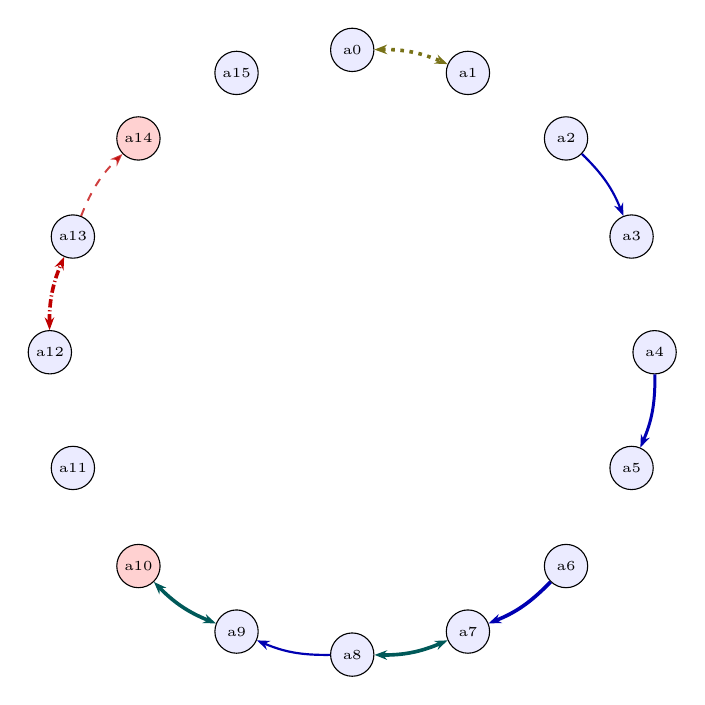
\begin{tikzpicture}[>={Stealth[length=1.6mm]}]
  \node[circle,draw,fill=blue!8,inner sep=1pt,minimum size=5.5mm,font=\tiny] (a0) at (90.0:3.84) {a0};
  \node[circle,draw,fill=blue!8,inner sep=1pt,minimum size=5.5mm,font=\tiny] (a1) at (67.5:3.84) {a1};
  \node[circle,draw,fill=blue!8,inner sep=1pt,minimum size=5.5mm,font=\tiny] (a2) at (45.0:3.84) {a2};
  \node[circle,draw,fill=blue!8,inner sep=1pt,minimum size=5.5mm,font=\tiny] (a3) at (22.5:3.84) {a3};
  \node[circle,draw,fill=blue!8,inner sep=1pt,minimum size=5.5mm,font=\tiny] (a4) at (0.0:3.84) {a4};
  \node[circle,draw,fill=blue!8,inner sep=1pt,minimum size=5.5mm,font=\tiny] (a5) at (-22.5:3.84) {a5};
  \node[circle,draw,fill=blue!8,inner sep=1pt,minimum size=5.5mm,font=\tiny] (a6) at (-45.0:3.84) {a6};
  \node[circle,draw,fill=blue!8,inner sep=1pt,minimum size=5.5mm,font=\tiny] (a7) at (-67.5:3.84) {a7};
  \node[circle,draw,fill=blue!8,inner sep=1pt,minimum size=5.5mm,font=\tiny] (a8) at (-90.0:3.84) {a8};
  \node[circle,draw,fill=blue!8,inner sep=1pt,minimum size=5.5mm,font=\tiny] (a9) at (-112.5:3.84) {a9};
  \node[circle,draw,fill=red!18,inner sep=1pt,minimum size=5.5mm,font=\tiny] (a10) at (-135.0:3.84) {a10};
  \node[circle,draw,fill=blue!8,inner sep=1pt,minimum size=5.5mm,font=\tiny] (a11) at (-157.5:3.84) {a11};
  \node[circle,draw,fill=blue!8,inner sep=1pt,minimum size=5.5mm,font=\tiny] (a12) at (-180.0:3.84) {a12};
  \node[circle,draw,fill=blue!8,inner sep=1pt,minimum size=5.5mm,font=\tiny] (a13) at (-202.5:3.84) {a13};
  \node[circle,draw,fill=red!18,inner sep=1pt,minimum size=5.5mm,font=\tiny] (a14) at (-225.0:3.84) {a14};
  \node[circle,draw,fill=blue!8,inner sep=1pt,minimum size=5.5mm,font=\tiny] (a15) at (-247.5:3.84) {a15};
  \draw[{Stealth[length=1.6mm]}-{Stealth[length=1.6mm]}, olive!80!black, dotted, line width=1.31pt] (a0) to[bend left=12] (a1);
  \draw[-{Stealth[length=1.6mm]}, blue!70!black, line width=0.79pt] (a2) to[bend left=12] (a3);
  \draw[-{Stealth[length=1.6mm]}, blue!70!black, line width=1.08pt] (a4) to[bend left=12] (a5);
  \draw[-{Stealth[length=1.6mm]}, blue!70!black, line width=1.31pt] (a6) to[bend left=12] (a7);
  \draw[{Stealth[length=1.6mm]}-{Stealth[length=1.6mm]}, teal!70!black, line width=1.31pt] (a7) to[bend left=12] (a8);
  \draw[-{Stealth[length=1.6mm]}, blue!70!black, line width=0.79pt] (a8) to[bend left=12] (a9);
  \draw[{Stealth[length=1.6mm]}-{Stealth[length=1.6mm]}, teal!70!black, line width=1.31pt] (a9) to[bend left=12] (a10);
  \draw[{Stealth[length=1.6mm]}-{Stealth[length=1.6mm]}, red!75!black, densely dashdotted, line width=1.31pt] (a12) to[bend left=12] (a13);
  \draw[-{Stealth[length=1.6mm]}, red!75!black, dashed, opacity=0.75, line width=0.71pt] (a13) to[bend left=12] (a14);
\end{tikzpicture}
}
\\[2pt]{\footnotesize all gold edges: 9 factors}
\end{minipage}\hfill\begin{minipage}[t]{0.48\linewidth}\centering
\resizebox{!}{6.4cm}{%
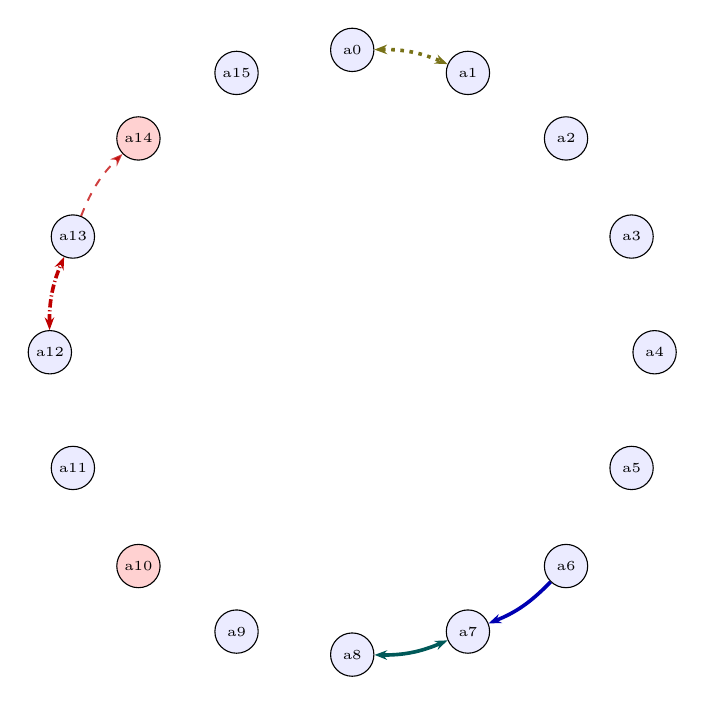
\begin{tikzpicture}[>={Stealth[length=1.6mm]}]
  \node[circle,draw,fill=blue!8,inner sep=1pt,minimum size=5.5mm,font=\tiny] (a0) at (90.0:3.84) {a0};
  \node[circle,draw,fill=blue!8,inner sep=1pt,minimum size=5.5mm,font=\tiny] (a1) at (67.5:3.84) {a1};
  \node[circle,draw,fill=blue!8,inner sep=1pt,minimum size=5.5mm,font=\tiny] (a2) at (45.0:3.84) {a2};
  \node[circle,draw,fill=blue!8,inner sep=1pt,minimum size=5.5mm,font=\tiny] (a3) at (22.5:3.84) {a3};
  \node[circle,draw,fill=blue!8,inner sep=1pt,minimum size=5.5mm,font=\tiny] (a4) at (0.0:3.84) {a4};
  \node[circle,draw,fill=blue!8,inner sep=1pt,minimum size=5.5mm,font=\tiny] (a5) at (-22.5:3.84) {a5};
  \node[circle,draw,fill=blue!8,inner sep=1pt,minimum size=5.5mm,font=\tiny] (a6) at (-45.0:3.84) {a6};
  \node[circle,draw,fill=blue!8,inner sep=1pt,minimum size=5.5mm,font=\tiny] (a7) at (-67.5:3.84) {a7};
  \node[circle,draw,fill=blue!8,inner sep=1pt,minimum size=5.5mm,font=\tiny] (a8) at (-90.0:3.84) {a8};
  \node[circle,draw,fill=blue!8,inner sep=1pt,minimum size=5.5mm,font=\tiny] (a9) at (-112.5:3.84) {a9};
  \node[circle,draw,fill=red!18,inner sep=1pt,minimum size=5.5mm,font=\tiny] (a10) at (-135.0:3.84) {a10};
  \node[circle,draw,fill=blue!8,inner sep=1pt,minimum size=5.5mm,font=\tiny] (a11) at (-157.5:3.84) {a11};
  \node[circle,draw,fill=blue!8,inner sep=1pt,minimum size=5.5mm,font=\tiny] (a12) at (-180.0:3.84) {a12};
  \node[circle,draw,fill=blue!8,inner sep=1pt,minimum size=5.5mm,font=\tiny] (a13) at (-202.5:3.84) {a13};
  \node[circle,draw,fill=red!18,inner sep=1pt,minimum size=5.5mm,font=\tiny] (a14) at (-225.0:3.84) {a14};
  \node[circle,draw,fill=blue!8,inner sep=1pt,minimum size=5.5mm,font=\tiny] (a15) at (-247.5:3.84) {a15};
  \draw[{Stealth[length=1.6mm]}-{Stealth[length=1.6mm]}, olive!80!black, dotted, line width=1.31pt] (a0) to[bend left=12] (a1);
  \draw[-{Stealth[length=1.6mm]}, blue!70!black, line width=1.31pt] (a6) to[bend left=12] (a7);
  \draw[{Stealth[length=1.6mm]}-{Stealth[length=1.6mm]}, teal!70!black, line width=1.31pt] (a7) to[bend left=12] (a8);
  \draw[{Stealth[length=1.6mm]}-{Stealth[length=1.6mm]}, red!75!black, densely dashdotted, line width=1.31pt] (a12) to[bend left=12] (a13);
  \draw[-{Stealth[length=1.6mm]}, red!75!black, dashed, opacity=0.75, line width=0.71pt] (a13) to[bend left=12] (a14);
\end{tikzpicture}
}
\\[2pt]{\footnotesize valid edges only: 5 factors}
\end{minipage}
\caption{Relation graph for \texttt{locobench-claude-5-fixed-f004-r1}. Nodes are atoms on a circle, tinted red when the item marks them non-factual (prior 0.1) and blue when factual (prior 0.9). Edges are gold relations: solid blue = entailment, dashed red = contradiction, double-headed teal = equivalence, dash-dotted red (double-headed) = exclusive (exactly-one), dotted olive (double-headed) = co-necessity (at-least-one); thickness scales with the factor probability. Ordering-only Precedence edges carry no factor and so are not drawn.}
\label{fig:graph-locobench-claude-5-fixed-f004-r1}
\end{figure}

\begin{table}[htbp]
\centering
\footnotesize
\setlength{\tabcolsep}{3.5pt}
\caption{The specific gold relations of \texttt{locobench-claude-5-fixed-f004-r1}. \textbf{$p$ used} is the factor probability the MRF received: the band midpoint, times $(1-\lambda)$ for a resolved concession, or \emph{none} for an ordering-only edge (no factor). \textbf{Valid} marks the deliberately-planted errors with their kind. \textbf{Res.} is the resolving atom of a resolved concession.}
\label{tab:rels-locobench-claude-5-fixed-f004-r1}
\begin{tabular}{lllllrll}
\toprule
ID & Endpoints & Sense & Coupling & Band & $p$ used & Valid & Res. \\
\midrule
\texttt{r000} & \texttt{a0} $\leftrightarrow$ \texttt{a1} & Disjunction & \texttt{co\_necessity} & strong & 0.925 & \checkmark &  \\
\texttt{r001} & \texttt{a2} $\to$ \texttt{a3} & Instantiation & \texttt{entailment} & weak & 0.470 & $\times$ {\scriptsize wrong\_sense} &  \\
\texttt{r002} & \texttt{a4} $\to$ \texttt{a5} & Cause-Effect & \texttt{entailment} & moderate & 0.720 & $\times$ {\scriptsize wrong\_sense} &  \\
\texttt{r003} & \texttt{a6} $\to$ \texttt{a7} & Evidence & \texttt{entailment} & strong & 0.925 & \checkmark &  \\
\texttt{r004} & \texttt{a7} $\leftrightarrow$ \texttt{a8} & Restatement & \texttt{equivalence} & strong & 0.925 & \checkmark &  \\
\texttt{r005} & \texttt{a8} $\to$ \texttt{a9} & Instantiation & \texttt{entailment} & weak & 0.470 & $\times$ {\scriptsize spurious} &  \\
\texttt{r006} & \texttt{a9} $\leftrightarrow$ \texttt{a10} & Restatement & \texttt{equivalence} & strong & 0.925 & $\times$ {\scriptsize false\_endpoint} &  \\
\texttt{r007} & \texttt{a11} $\to$ \texttt{a13} & Precedence & \texttt{none} & moderate & \emph{none} & \checkmark &  \\
\texttt{r008} & \texttt{a12} $\leftrightarrow$ \texttt{a13} & Alternative & \texttt{exclusive} & strong & 0.925 & \checkmark &  \\
\texttt{r009} & \texttt{a13} $\to$ \texttt{a14} & Concession & \texttt{contradiction} & moderate & 0.396 & \checkmark & \texttt{a15} \\
\bottomrule
\end{tabular}
\end{table}

\begin{table}[htbp]
\centering
\footnotesize
\caption{Atoms of \texttt{locobench-claude-5-fixed-f004-r1}: the \texttt{factual} label, the prior it maps to, the posterior marginal $P(a_i{=}1)$ the MRF returns, and the shift. Atoms dragged below their prior are the ones the coherence structure penalises.}
\label{tab:atoms-locobench-claude-5-fixed-f004-r1}
\begin{tabular}{llrrrp{7.2cm}}
\toprule
Atom & fact & $\pi_i$ & $P(a_i{=}1)$ & $\Delta$ & Text \\
\midrule
\texttt{a0} & \checkmark & 0.90 & 0.946 & +0.046 & \footnotesize The model's high benchmark score rests on exposure to the benchmark's items during training. \\
\texttt{a1} & \checkmark & 0.90 & 0.946 & +0.046 & \footnotesize The model's high benchmark score rests on reasoning ability that transfers to unseen problems. \\
\texttt{a2} & \checkmark & 0.90 & 0.895 & -0.005 & \footnotesize Researchers compute n-gram overlap between benchmark items and pretraining corpora to estimate contamination. \\
\texttt{a3} & \checkmark & 0.90 & 0.890 & -0.010 & \footnotesize Proprietary models with undisclosed training corpora cannot be audited by direct string-overlap checks. \\
\texttt{a4} & \checkmark & 0.90 & 0.924 & +0.024 & \footnotesize Membership inference methods such as Min-K\% Prob estimate whether a particular example appeared in a model's training data. \\
\texttt{a5} & \checkmark & 0.90 & 0.954 & +0.054 & \footnotesize Min-K\% Prob operates using only the token-level log probabilities returned by the model. \\
\texttt{a6} & \checkmark & 0.90 & 0.942 & +0.042 & \footnotesize Systematically lower loss on benchmark test items than on comparably difficult unseen items indicates that the items were seen during training. \\
\texttt{a7} & \checkmark & 0.90 & 0.997 & +0.097 & \footnotesize The benchmark's test items leaked into the model's training corpus. \\
\texttt{a8} & \checkmark & 0.90 & 0.989 & +0.089 & \footnotesize The model was trained on data that contained the benchmark's test items. \\
\texttt{a9} & \checkmark & 0.90 & 0.604 & -0.296 & \footnotesize GSM8K is a dataset of roughly 8,500 grade-school math word problems released by OpenAI in 2021. \\
\texttt{a10} & $\times$ & 0.10 & 0.352 & +0.252 & \footnotesize GSM8K was released by DeepMind in 2018. \\
\texttt{a11} & \checkmark & 0.90 & 0.900 & +0.000 & \footnotesize Scale AI constructed GSM1k, a set of 1,250 new grade-school math problems designed to mirror the difficulty distribution of GSM8K. \\
\texttt{a12} & \checkmark & 0.90 & 0.656 & -0.244 & \footnotesize No model evaluated on GSM1k showed a meaningful accuracy drop relative to its GSM8K score. \\
\texttt{a13} & \checkmark & 0.90 & 0.588 & -0.312 & \footnotesize Several models evaluated on GSM1k showed accuracy drops of up to 13 percentage points relative to their GSM8K scores. \\
\texttt{a14} & $\times$ & 0.10 & 0.126 & +0.026 & \footnotesize The GSM1k evaluation found that GPT-4 and Claude exhibited the largest accuracy drops of all model families tested. \\
\texttt{a15} & \checkmark & 0.90 & 0.900 & +0.000 & \footnotesize The final GSM1k report concluded that frontier models from OpenAI, Anthropic, and Google showed minimal signs of overfitting to GSM8K. \\
\bottomrule
\end{tabular}
\end{table}

\subsection{Astronomy -- break\_2 (\texttt{locobench-claude-5-fixed-f005-r1})}

\textbf{Topic:} Astronomy (Natural Sciences). \textbf{Family:} \texttt{f005} (CHAIN), rung 1 (\emph{break\_2}). \textbf{Scores:} mean-marg $= 0.773$, consist $= 0.563$, reified $= 0.329$, log-Z $= 0.459$.



\paragraph{Framing question.} \emph{How did astronomers adjudicate between the competing accounts of the anomalous precession of Mercury's perihelion, and what settled which explanation could stand?}



\paragraph{Response.} {\small The dispute over the residual motion of Mercury's perihelion was settled not by any appeal to first principles but by the progressive elimination of proposed material causes, until only one candidate explanation remained standing. Urbain Le Verrier reported an anomalous advance of Mercury's perihelion in 1859, and that report rested on no such ground: he separately derived the anomaly from an analysis of recorded transits of Mercury across the solar disk, and that analysis is not evidence for the report at all.

The magnitude of the effect fixed the terms of every subsequent debate. The unexplained advance of Mercury's perihelion amounts to about 43 arcseconds per century; equivalently, the perihelion drifts forward by roughly 43 seconds of arc each hundred years beyond the Newtonian prediction. That figure is minute against the planet's total observed precession, most of which is attributable to the perturbations of Venus, Earth and Jupiter, and it proved remarkably stable as successive ephemerides refined the planetary masses through the nineteenth century. Any admissible mechanism therefore had to deliver a very small, very specific secular term without disturbing the well-fitted motions of the other inner planets. The 1859 announcement of the discrepancy led its author to propose an unseen intramercurial planet, later named Vulcan, as the cause of the residual motion; by contrast, he accounted for the anomaly by positing an additional moon in orbit around Mercury.

Observational support for an intramercurial body was pursued vigorously and briefly seemed to arrive. Edmond Lescarbault reported seeing a dark round object cross the face of the Sun in 1859, a claim that came after astronomers had already mounted searches for an intramercurial planet during total solar eclipses in the 1870s and 1880s. Despite that solar-disk sighting, the two accounts on offer are mutually exclusive: either no intramercurial planet has ever been confirmed to exist, or a planet orbiting between Mercury and the Sun was confirmed by later observations, and while the two cannot both be true, one of them must hold. The tension is resolved by a subsequent assessment of the eclipse search records, which determined that the reported intramercurial objects were known stars; with the eclipse candidates reduced to misidentified field stars, the sighting on the solar disk carries no weight against the absence of any confirmed planet. That reassessment of the records is also what prompted astronomers to undertake the eclipse campaigns of those two decades.

A second material hypothesis appealed to diffuse matter rather than a discrete body. Hugo von Seeliger proposed that a distribution of zodiacal dust inside Mercury's orbit produced the residual advance; specifically, no ring of zodiacal dust of the density required to shift Mercury's perihelion lies inside Mercury's orbit. Nor was distributed matter the only Newtonian resource to fail, since at least one of two constraints holds, and perhaps both: the absence of such a dust ring, or the fact that the Sun's quadrupole moment is far too small to generate the observed residual advance. Either constraint suffices to close off the corresponding line of explanation, and jointly they exhaust the plausible sources of an unmodelled Newtonian torque within the inner solar system.

What remained was a modification of gravitation itself. Einstein presented a general-relativistic calculation of Mercury's perihelion advance in November 1915, obtaining the 43 arcseconds per century from the field equations with no adjustable parameter, which is why the result functioned as a decisive test rather than as a fit. Einstein published his treatment of Mercury's perihelion in his 1905 paper on special relativity. The adjudication thus rested on the failure of every hypothesized perturbing mass and on the exact agreement of a parameter-free prediction with a century of transit and meridian observations.}

\begin{figure}[htbp]
\centering
\begin{minipage}[t]{0.48\linewidth}\centering
\resizebox{!}{6.4cm}{%
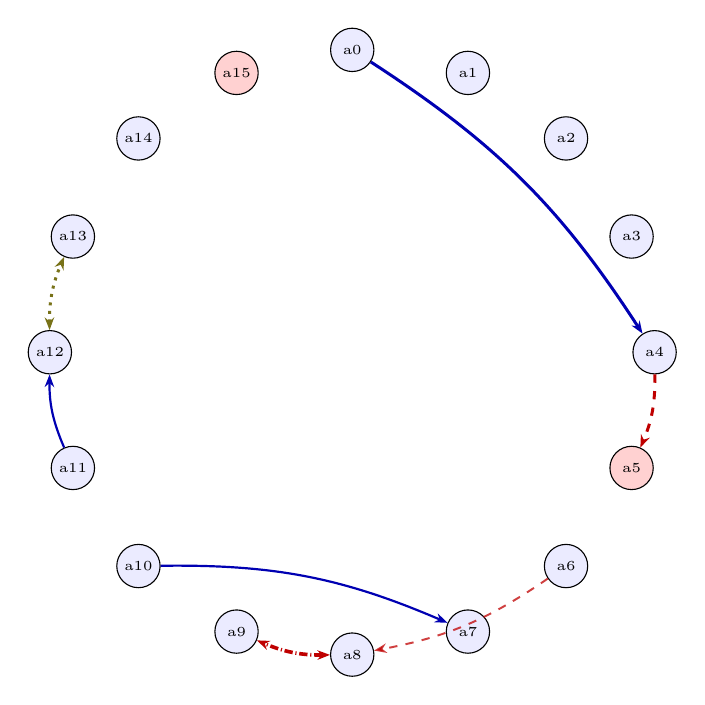
\begin{tikzpicture}[>={Stealth[length=1.6mm]}]
  \node[circle,draw,fill=blue!8,inner sep=1pt,minimum size=5.5mm,font=\tiny] (a0) at (90.0:3.84) {a0};
  \node[circle,draw,fill=blue!8,inner sep=1pt,minimum size=5.5mm,font=\tiny] (a1) at (67.5:3.84) {a1};
  \node[circle,draw,fill=blue!8,inner sep=1pt,minimum size=5.5mm,font=\tiny] (a2) at (45.0:3.84) {a2};
  \node[circle,draw,fill=blue!8,inner sep=1pt,minimum size=5.5mm,font=\tiny] (a3) at (22.5:3.84) {a3};
  \node[circle,draw,fill=blue!8,inner sep=1pt,minimum size=5.5mm,font=\tiny] (a4) at (0.0:3.84) {a4};
  \node[circle,draw,fill=red!18,inner sep=1pt,minimum size=5.5mm,font=\tiny] (a5) at (-22.5:3.84) {a5};
  \node[circle,draw,fill=blue!8,inner sep=1pt,minimum size=5.5mm,font=\tiny] (a6) at (-45.0:3.84) {a6};
  \node[circle,draw,fill=blue!8,inner sep=1pt,minimum size=5.5mm,font=\tiny] (a7) at (-67.5:3.84) {a7};
  \node[circle,draw,fill=blue!8,inner sep=1pt,minimum size=5.5mm,font=\tiny] (a8) at (-90.0:3.84) {a8};
  \node[circle,draw,fill=blue!8,inner sep=1pt,minimum size=5.5mm,font=\tiny] (a9) at (-112.5:3.84) {a9};
  \node[circle,draw,fill=blue!8,inner sep=1pt,minimum size=5.5mm,font=\tiny] (a10) at (-135.0:3.84) {a10};
  \node[circle,draw,fill=blue!8,inner sep=1pt,minimum size=5.5mm,font=\tiny] (a11) at (-157.5:3.84) {a11};
  \node[circle,draw,fill=blue!8,inner sep=1pt,minimum size=5.5mm,font=\tiny] (a12) at (-180.0:3.84) {a12};
  \node[circle,draw,fill=blue!8,inner sep=1pt,minimum size=5.5mm,font=\tiny] (a13) at (-202.5:3.84) {a13};
  \node[circle,draw,fill=blue!8,inner sep=1pt,minimum size=5.5mm,font=\tiny] (a14) at (-225.0:3.84) {a14};
  \node[circle,draw,fill=red!18,inner sep=1pt,minimum size=5.5mm,font=\tiny] (a15) at (-247.5:3.84) {a15};
  \draw[-{Stealth[length=1.6mm]}, blue!70!black, line width=1.08pt] (a0) to[bend left=12] (a4);
  \draw[-{Stealth[length=1.6mm]}, red!75!black, dashed, line width=1.08pt] (a4) to[bend left=12] (a5);
  \draw[{Stealth[length=1.6mm]}-{Stealth[length=1.6mm]}, red!75!black, densely dashdotted, line width=1.31pt] (a8) to[bend left=12] (a9);
  \draw[-{Stealth[length=1.6mm]}, red!75!black, dashed, opacity=0.75, line width=0.71pt] (a6) to[bend left=12] (a8);
  \draw[-{Stealth[length=1.6mm]}, blue!70!black, line width=0.79pt] (a10) to[bend left=12] (a7);
  \draw[-{Stealth[length=1.6mm]}, blue!70!black, line width=0.79pt] (a11) to[bend left=12] (a12);
  \draw[{Stealth[length=1.6mm]}-{Stealth[length=1.6mm]}, olive!80!black, dotted, line width=1.08pt] (a12) to[bend left=12] (a13);
\end{tikzpicture}
}
\\[2pt]{\footnotesize all gold edges: 7 factors}
\end{minipage}\hfill\begin{minipage}[t]{0.48\linewidth}\centering
\resizebox{!}{6.4cm}{%
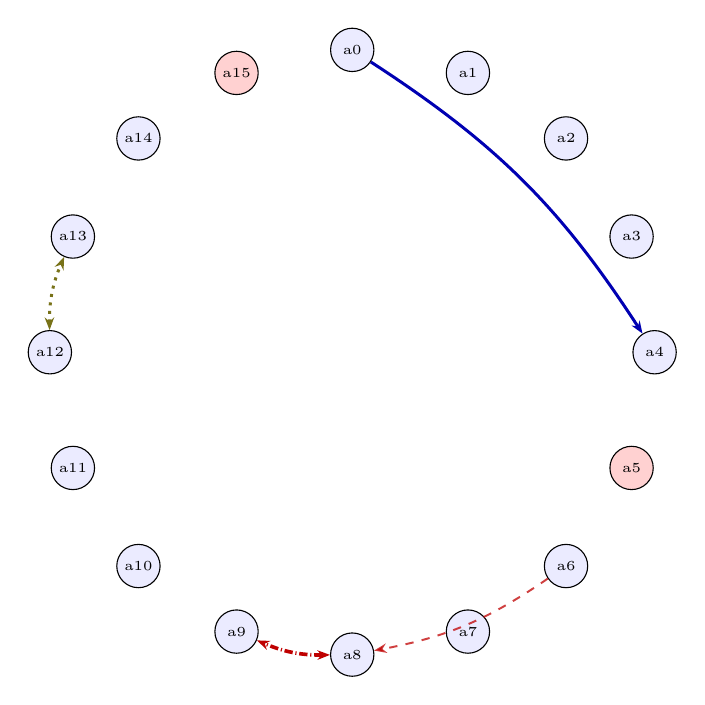
\begin{tikzpicture}[>={Stealth[length=1.6mm]}]
  \node[circle,draw,fill=blue!8,inner sep=1pt,minimum size=5.5mm,font=\tiny] (a0) at (90.0:3.84) {a0};
  \node[circle,draw,fill=blue!8,inner sep=1pt,minimum size=5.5mm,font=\tiny] (a1) at (67.5:3.84) {a1};
  \node[circle,draw,fill=blue!8,inner sep=1pt,minimum size=5.5mm,font=\tiny] (a2) at (45.0:3.84) {a2};
  \node[circle,draw,fill=blue!8,inner sep=1pt,minimum size=5.5mm,font=\tiny] (a3) at (22.5:3.84) {a3};
  \node[circle,draw,fill=blue!8,inner sep=1pt,minimum size=5.5mm,font=\tiny] (a4) at (0.0:3.84) {a4};
  \node[circle,draw,fill=red!18,inner sep=1pt,minimum size=5.5mm,font=\tiny] (a5) at (-22.5:3.84) {a5};
  \node[circle,draw,fill=blue!8,inner sep=1pt,minimum size=5.5mm,font=\tiny] (a6) at (-45.0:3.84) {a6};
  \node[circle,draw,fill=blue!8,inner sep=1pt,minimum size=5.5mm,font=\tiny] (a7) at (-67.5:3.84) {a7};
  \node[circle,draw,fill=blue!8,inner sep=1pt,minimum size=5.5mm,font=\tiny] (a8) at (-90.0:3.84) {a8};
  \node[circle,draw,fill=blue!8,inner sep=1pt,minimum size=5.5mm,font=\tiny] (a9) at (-112.5:3.84) {a9};
  \node[circle,draw,fill=blue!8,inner sep=1pt,minimum size=5.5mm,font=\tiny] (a10) at (-135.0:3.84) {a10};
  \node[circle,draw,fill=blue!8,inner sep=1pt,minimum size=5.5mm,font=\tiny] (a11) at (-157.5:3.84) {a11};
  \node[circle,draw,fill=blue!8,inner sep=1pt,minimum size=5.5mm,font=\tiny] (a12) at (-180.0:3.84) {a12};
  \node[circle,draw,fill=blue!8,inner sep=1pt,minimum size=5.5mm,font=\tiny] (a13) at (-202.5:3.84) {a13};
  \node[circle,draw,fill=blue!8,inner sep=1pt,minimum size=5.5mm,font=\tiny] (a14) at (-225.0:3.84) {a14};
  \node[circle,draw,fill=red!18,inner sep=1pt,minimum size=5.5mm,font=\tiny] (a15) at (-247.5:3.84) {a15};
  \draw[-{Stealth[length=1.6mm]}, blue!70!black, line width=1.08pt] (a0) to[bend left=12] (a4);
  \draw[{Stealth[length=1.6mm]}-{Stealth[length=1.6mm]}, red!75!black, densely dashdotted, line width=1.31pt] (a8) to[bend left=12] (a9);
  \draw[-{Stealth[length=1.6mm]}, red!75!black, dashed, opacity=0.75, line width=0.71pt] (a6) to[bend left=12] (a8);
  \draw[{Stealth[length=1.6mm]}-{Stealth[length=1.6mm]}, olive!80!black, dotted, line width=1.08pt] (a12) to[bend left=12] (a13);
\end{tikzpicture}
}
\\[2pt]{\footnotesize valid edges only: 4 factors}
\end{minipage}
\caption{Relation graph for \texttt{locobench-claude-5-fixed-f005-r1}. Nodes are atoms on a circle, tinted red when the item marks them non-factual (prior 0.1) and blue when factual (prior 0.9). Edges are gold relations: solid blue = entailment, dashed red = contradiction, double-headed teal = equivalence, dash-dotted red (double-headed) = exclusive (exactly-one), dotted olive (double-headed) = co-necessity (at-least-one); thickness scales with the factor probability. Ordering-only Precedence edges carry no factor and so are not drawn.}
\label{fig:graph-locobench-claude-5-fixed-f005-r1}
\end{figure}

\begin{table}[htbp]
\centering
\footnotesize
\setlength{\tabcolsep}{3.5pt}
\caption{The specific gold relations of \texttt{locobench-claude-5-fixed-f005-r1}. \textbf{$p$ used} is the factor probability the MRF received: the band midpoint, times $(1-\lambda)$ for a resolved concession, or \emph{none} for an ordering-only edge (no factor). \textbf{Valid} marks the deliberately-planted errors with their kind. \textbf{Res.} is the resolving atom of a resolved concession.}
\label{tab:rels-locobench-claude-5-fixed-f005-r1}
\begin{tabular}{lllllrll}
\toprule
ID & Endpoints & Sense & Coupling & Band & $p$ used & Valid & Res. \\
\midrule
\texttt{r002} & \texttt{a0} $\to$ \texttt{a4} & Cause-Effect & \texttt{entailment} & moderate & 0.720 & \checkmark &  \\
\texttt{r003} & \texttt{a4} $\leftrightarrow$ \texttt{a5} & Contrast & \texttt{contradiction} & moderate & 0.720 & $\times$ {\scriptsize false\_endpoint} &  \\
\texttt{r004} & \texttt{a6} $\to$ \texttt{a7} & Succession & \texttt{none} & moderate & \emph{none} & $\times$ {\scriptsize wrong\_direction} &  \\
\texttt{r005} & \texttt{a8} $\leftrightarrow$ \texttt{a9} & Alternative & \texttt{exclusive} & strong & 0.925 & \checkmark &  \\
\texttt{r006} & \texttt{a6} $\to$ \texttt{a8} & Concession & \texttt{contradiction} & moderate & 0.396 & \checkmark & \texttt{a10} \\
\texttt{r007} & \texttt{a10} $\to$ \texttt{a7} & Cause-Effect & \texttt{entailment} & weak & 0.470 & $\times$ {\scriptsize wrong\_direction} &  \\
\texttt{r008} & \texttt{a11} $\to$ \texttt{a12} & Instantiation & \texttt{entailment} & weak & 0.470 & $\times$ {\scriptsize wrong\_sense} &  \\
\texttt{r009} & \texttt{a12} $\leftrightarrow$ \texttt{a13} & Disjunction & \texttt{co\_necessity} & moderate & 0.720 & \checkmark &  \\
\bottomrule
\end{tabular}
\end{table}

\begin{table}[htbp]
\centering
\footnotesize
\caption{Atoms of \texttt{locobench-claude-5-fixed-f005-r1}: the \texttt{factual} label, the prior it maps to, the posterior marginal $P(a_i{=}1)$ the MRF returns, and the shift. Atoms dragged below their prior are the ones the coherence structure penalises.}
\label{tab:atoms-locobench-claude-5-fixed-f005-r1}
\begin{tabular}{llrrrp{7.2cm}}
\toprule
Atom & fact & $\pi_i$ & $P(a_i{=}1)$ & $\Delta$ & Text \\
\midrule
\texttt{a0} & \checkmark & 0.90 & 0.925 & +0.025 & \footnotesize Urbain Le Verrier reported an anomalous advance of Mercury's perihelion in 1859. \\
\texttt{a1} & \checkmark & 0.90 & 0.900 & +0.000 & \footnotesize Le Verrier derived the anomaly from an analysis of recorded transits of Mercury across the solar disk. \\
\texttt{a2} & \checkmark & 0.90 & 0.900 & +0.000 & \footnotesize The unexplained advance of Mercury's perihelion amounts to about 43 arcseconds per century. \\
\texttt{a3} & \checkmark & 0.90 & 0.900 & +0.000 & \footnotesize Mercury's perihelion drifts forward by roughly 43 seconds of arc each hundred years beyond the Newtonian prediction. \\
\texttt{a4} & \checkmark & 0.90 & 0.966 & +0.066 & \footnotesize Le Verrier proposed an unseen intramercurial planet, later named Vulcan, as the cause of the residual motion. \\
\texttt{a5} & $\times$ & 0.10 & 0.043 & -0.057 & \footnotesize Le Verrier accounted for the anomaly by positing an additional moon in orbit around Mercury. \\
\texttt{a6} & \checkmark & 0.90 & 0.905 & +0.005 & \footnotesize Edmond Lescarbault reported seeing a dark round object cross the face of the Sun in 1859. \\
\texttt{a7} & \checkmark & 0.90 & 0.890 & -0.010 & \footnotesize Astronomers mounted searches for an intramercurial planet during total solar eclipses in the 1870s and 1880s. \\
\texttt{a8} & \checkmark & 0.90 & 0.715 & -0.185 & \footnotesize No intramercurial planet has ever been confirmed to exist. \\
\texttt{a9} & \checkmark & 0.90 & 0.584 & -0.316 & \footnotesize A planet orbiting between Mercury and the Sun was confirmed by later observations. \\
\texttt{a10} & \checkmark & 0.90 & 0.895 & -0.005 & \footnotesize A subsequent assessment of the eclipse search records determined that the reported intramercurial objects were known stars. \\
\texttt{a11} & \checkmark & 0.90 & 0.895 & -0.005 & \footnotesize Hugo von Seeliger proposed that a distribution of zodiacal dust inside Mercury's orbit produced the residual advance. \\
\texttt{a12} & \checkmark & 0.90 & 0.922 & +0.022 & \footnotesize No ring of zodiacal dust of the density required to shift Mercury's perihelion lies inside Mercury's orbit. \\
\texttt{a13} & \checkmark & 0.90 & 0.929 & +0.029 & \footnotesize The Sun's quadrupole moment is far too small to generate the observed residual advance. \\
\texttt{a14} & \checkmark & 0.90 & 0.900 & +0.000 & \footnotesize Einstein presented a general-relativistic calculation of Mercury's perihelion advance in November 1915. \\
\texttt{a15} & $\times$ & 0.10 & 0.100 & +0.000 & \footnotesize Einstein published his treatment of Mercury's perihelion in his 1905 paper on special relativity. \\
\bottomrule
\end{tabular}
\end{table}

\subsection{Botany -- shuffle\_block (\texttt{locobench-claude-5-fixed-f007-r1})}

\textbf{Topic:} Botany (Natural Sciences). \textbf{Family:} \texttt{f007} (ORDER), rung 1 (\emph{shuffle\_block}). \textbf{Scores:} mean-marg $= 0.784$, consist $= 0.491$, reified $= 0.184$, log-Z $= 0.442$.



\paragraph{Framing question.} \emph{How do botanists adjudicate between an introduced pathogen and drought-driven physiological failure when a forest stand shows sudden, widespread dieback of uncertain origin?}



\paragraph{Response.} {\small Quantifying that stress requires instrumentation. Predawn leaf water potential is measured with a pressure chamber to quantify tree water stress, and because such measurements are made, tree-ring chronologies reveal multi-year growth declines preceding drought-related mortality. Those ring-width declines are themselves the strongest available evidence that the stand experienced a multi-year rainfall deficit in the years preceding the dieback, since the annual increment integrates growing-season moisture supply in a way no single-season observation can. Once that deficit is established, the two candidate explanations cease to be mutually exclusive: at least one of the following held in this stand, and perhaps both — the multi-year rainfall deficit already documented in the ring series, or the establishment of a non-native pathogen in the stand's soil and bark tissue. The quantitative extent of the damage constrains how much either factor must explain. The dieback affected 40 percent of the stems in the stand; in other words, two of every five stems showed dieback, a proportion too large to be dismissed as background mortality and too small to indicate uniform stand-wide hydraulic collapse.

The inferential weight carried by a positive result is where most disputes arise. Detection of pathogen DNA in symptomatic tissue by itself satisfies Koch's postulates. Koch's postulates, by contrast, require reisolation of the suspected pathogen from experimentally inoculated healthy plants, so that the organism recovered at the end of the experiment is shown to be the organism introduced at its beginning. A stand-level attribution that rests on molecular detection alone therefore occupies a different evidentiary position from one supported by completed inoculation trials, and the distinction should be stated explicitly in any report.

What ultimately separates the two accounts is chronology, because a pathogen that arrived only after the crowns had begun to thin cannot be the initiating agent, whereas one already resident when the deficit began is a plausible co-factor. Either the pathogen was present in the stand before the onset of the dieback, or, despite its establishment in the soil and bark tissue, it was absent from the stand before that onset; the two cannot both be true, and one of them must hold. Soil-baiting surveys of adjacent unaffected compartments, archived bark samples, and the spatial autocorrelation of symptomatic stems are the usual means of deciding between them. Here the question was answered directly: the final report determined that the pathogen was already established in the stand before the dieback began, which resolves the apparent conflict in favour of prior residency and licenses a combined attribution in which moisture deficit predisposed trees that a resident pathogen then killed.

When a stand collapses without an obvious cause, the adjudication between an introduced pathogen and drought-driven physiological failure proceeds as two parallel diagnostic programmes, each with its own evidentiary standard, and the two are then compared against the stand's history. The pathogen programme is anchored in lesion morphology. Bleeding cankers on the lower trunk are a diagnostic symptom of sudden oak death, and the field recording of such lesions precedes the laboratory stage at which selective media such as PARP agar are used to recover Phytophthora species from symptomatic bark tissue. Either that culture-based recovery is pursued, or quantitative PCR assays detect pathogen DNA in samples of diseased phloem; exactly one of the two routes is taken, and never both.

The physiological programme addresses the alternative explanation on its own terms. Drought-induced tree mortality proceeds through hydraulic failure caused by embolism in the xylem; that is, drought stress kills trees by inducing cavitation in the phloem. The mechanism matters for adjudication because it predicts a characteristic distribution of symptoms — crown dieback proportional to the hydraulic path length and to exposure — that differs from the patchy, inoculum-centred distribution expected of a soilborne or bark-invading pathogen.}

\begin{figure}[htbp]
\centering
\begin{minipage}[t]{0.48\linewidth}\centering
\resizebox{!}{6.4cm}{%
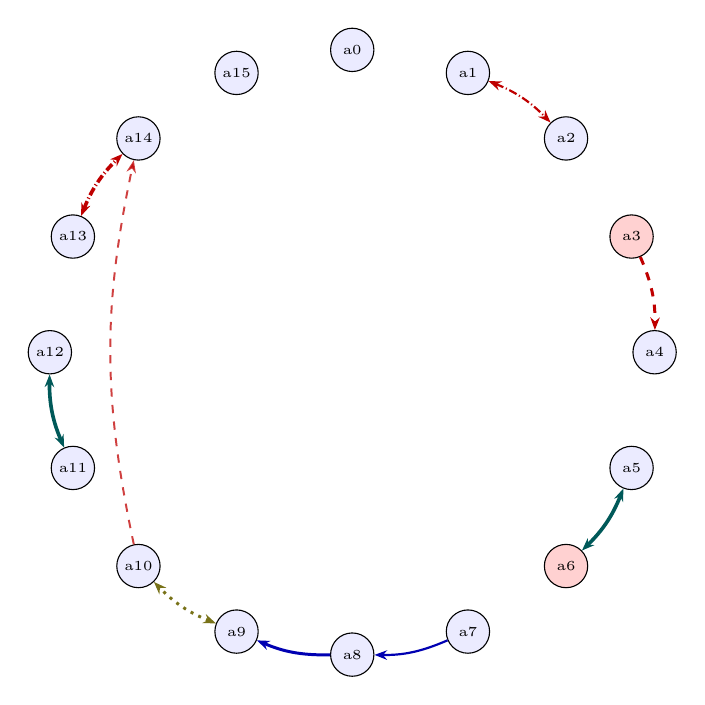
\begin{tikzpicture}[>={Stealth[length=1.6mm]}]
  \node[circle,draw,fill=blue!8,inner sep=1pt,minimum size=5.5mm,font=\tiny] (a0) at (90.0:3.84) {a0};
  \node[circle,draw,fill=blue!8,inner sep=1pt,minimum size=5.5mm,font=\tiny] (a1) at (67.5:3.84) {a1};
  \node[circle,draw,fill=blue!8,inner sep=1pt,minimum size=5.5mm,font=\tiny] (a2) at (45.0:3.84) {a2};
  \node[circle,draw,fill=red!18,inner sep=1pt,minimum size=5.5mm,font=\tiny] (a3) at (22.5:3.84) {a3};
  \node[circle,draw,fill=blue!8,inner sep=1pt,minimum size=5.5mm,font=\tiny] (a4) at (0.0:3.84) {a4};
  \node[circle,draw,fill=blue!8,inner sep=1pt,minimum size=5.5mm,font=\tiny] (a5) at (-22.5:3.84) {a5};
  \node[circle,draw,fill=red!18,inner sep=1pt,minimum size=5.5mm,font=\tiny] (a6) at (-45.0:3.84) {a6};
  \node[circle,draw,fill=blue!8,inner sep=1pt,minimum size=5.5mm,font=\tiny] (a7) at (-67.5:3.84) {a7};
  \node[circle,draw,fill=blue!8,inner sep=1pt,minimum size=5.5mm,font=\tiny] (a8) at (-90.0:3.84) {a8};
  \node[circle,draw,fill=blue!8,inner sep=1pt,minimum size=5.5mm,font=\tiny] (a9) at (-112.5:3.84) {a9};
  \node[circle,draw,fill=blue!8,inner sep=1pt,minimum size=5.5mm,font=\tiny] (a10) at (-135.0:3.84) {a10};
  \node[circle,draw,fill=blue!8,inner sep=1pt,minimum size=5.5mm,font=\tiny] (a11) at (-157.5:3.84) {a11};
  \node[circle,draw,fill=blue!8,inner sep=1pt,minimum size=5.5mm,font=\tiny] (a12) at (-180.0:3.84) {a12};
  \node[circle,draw,fill=blue!8,inner sep=1pt,minimum size=5.5mm,font=\tiny] (a13) at (-202.5:3.84) {a13};
  \node[circle,draw,fill=blue!8,inner sep=1pt,minimum size=5.5mm,font=\tiny] (a14) at (-225.0:3.84) {a14};
  \node[circle,draw,fill=blue!8,inner sep=1pt,minimum size=5.5mm,font=\tiny] (a15) at (-247.5:3.84) {a15};
  \draw[{Stealth[length=1.6mm]}-{Stealth[length=1.6mm]}, red!75!black, densely dashdotted, line width=0.79pt] (a1) to[bend left=12] (a2);
  \draw[-{Stealth[length=1.6mm]}, red!75!black, dashed, line width=1.08pt] (a3) to[bend left=12] (a4);
  \draw[{Stealth[length=1.6mm]}-{Stealth[length=1.6mm]}, teal!70!black, line width=1.31pt] (a5) to[bend left=12] (a6);
  \draw[-{Stealth[length=1.6mm]}, blue!70!black, line width=0.79pt] (a7) to[bend left=12] (a8);
  \draw[-{Stealth[length=1.6mm]}, blue!70!black, line width=1.08pt] (a8) to[bend left=12] (a9);
  \draw[{Stealth[length=1.6mm]}-{Stealth[length=1.6mm]}, olive!80!black, dotted, line width=1.08pt] (a9) to[bend left=12] (a10);
  \draw[-{Stealth[length=1.6mm]}, red!75!black, dashed, opacity=0.75, line width=0.71pt] (a10) to[bend left=12] (a14);
  \draw[{Stealth[length=1.6mm]}-{Stealth[length=1.6mm]}, teal!70!black, line width=1.31pt] (a11) to[bend left=12] (a12);
  \draw[{Stealth[length=1.6mm]}-{Stealth[length=1.6mm]}, red!75!black, densely dashdotted, line width=1.31pt] (a13) to[bend left=12] (a14);
\end{tikzpicture}
}
\\[2pt]{\footnotesize all gold edges: 9 factors}
\end{minipage}\hfill\begin{minipage}[t]{0.48\linewidth}\centering
\resizebox{!}{6.4cm}{%
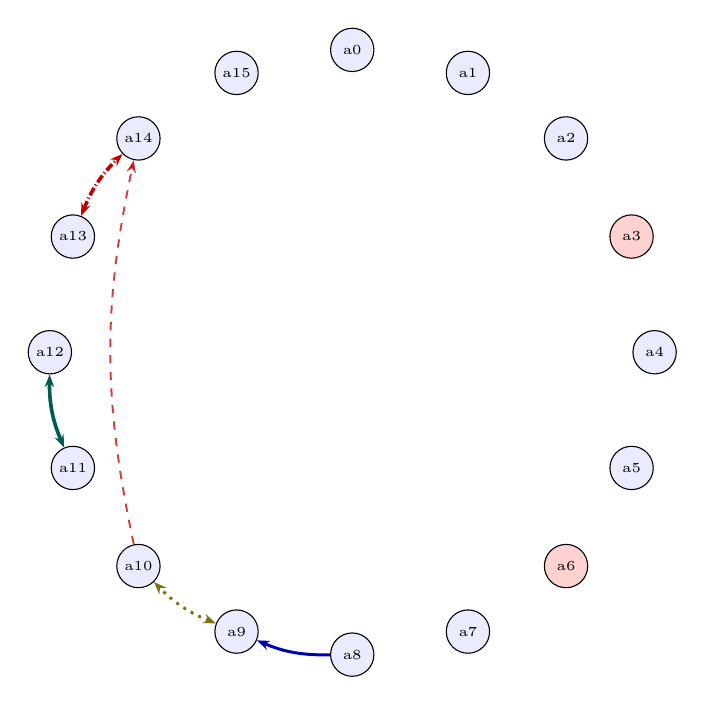
\begin{tikzpicture}[>={Stealth[length=1.6mm]}]
  \node[circle,draw,fill=blue!8,inner sep=1pt,minimum size=5.5mm,font=\tiny] (a0) at (90.0:3.84) {a0};
  \node[circle,draw,fill=blue!8,inner sep=1pt,minimum size=5.5mm,font=\tiny] (a1) at (67.5:3.84) {a1};
  \node[circle,draw,fill=blue!8,inner sep=1pt,minimum size=5.5mm,font=\tiny] (a2) at (45.0:3.84) {a2};
  \node[circle,draw,fill=red!18,inner sep=1pt,minimum size=5.5mm,font=\tiny] (a3) at (22.5:3.84) {a3};
  \node[circle,draw,fill=blue!8,inner sep=1pt,minimum size=5.5mm,font=\tiny] (a4) at (0.0:3.84) {a4};
  \node[circle,draw,fill=blue!8,inner sep=1pt,minimum size=5.5mm,font=\tiny] (a5) at (-22.5:3.84) {a5};
  \node[circle,draw,fill=red!18,inner sep=1pt,minimum size=5.5mm,font=\tiny] (a6) at (-45.0:3.84) {a6};
  \node[circle,draw,fill=blue!8,inner sep=1pt,minimum size=5.5mm,font=\tiny] (a7) at (-67.5:3.84) {a7};
  \node[circle,draw,fill=blue!8,inner sep=1pt,minimum size=5.5mm,font=\tiny] (a8) at (-90.0:3.84) {a8};
  \node[circle,draw,fill=blue!8,inner sep=1pt,minimum size=5.5mm,font=\tiny] (a9) at (-112.5:3.84) {a9};
  \node[circle,draw,fill=blue!8,inner sep=1pt,minimum size=5.5mm,font=\tiny] (a10) at (-135.0:3.84) {a10};
  \node[circle,draw,fill=blue!8,inner sep=1pt,minimum size=5.5mm,font=\tiny] (a11) at (-157.5:3.84) {a11};
  \node[circle,draw,fill=blue!8,inner sep=1pt,minimum size=5.5mm,font=\tiny] (a12) at (-180.0:3.84) {a12};
  \node[circle,draw,fill=blue!8,inner sep=1pt,minimum size=5.5mm,font=\tiny] (a13) at (-202.5:3.84) {a13};
  \node[circle,draw,fill=blue!8,inner sep=1pt,minimum size=5.5mm,font=\tiny] (a14) at (-225.0:3.84) {a14};
  \node[circle,draw,fill=blue!8,inner sep=1pt,minimum size=5.5mm,font=\tiny] (a15) at (-247.5:3.84) {a15};
  \draw[-{Stealth[length=1.6mm]}, blue!70!black, line width=1.08pt] (a8) to[bend left=12] (a9);
  \draw[{Stealth[length=1.6mm]}-{Stealth[length=1.6mm]}, olive!80!black, dotted, line width=1.08pt] (a9) to[bend left=12] (a10);
  \draw[-{Stealth[length=1.6mm]}, red!75!black, dashed, opacity=0.75, line width=0.71pt] (a10) to[bend left=12] (a14);
  \draw[{Stealth[length=1.6mm]}-{Stealth[length=1.6mm]}, teal!70!black, line width=1.31pt] (a11) to[bend left=12] (a12);
  \draw[{Stealth[length=1.6mm]}-{Stealth[length=1.6mm]}, red!75!black, densely dashdotted, line width=1.31pt] (a13) to[bend left=12] (a14);
\end{tikzpicture}
}
\\[2pt]{\footnotesize valid edges only: 5 factors}
\end{minipage}
\caption{Relation graph for \texttt{locobench-claude-5-fixed-f007-r1}. Nodes are atoms on a circle, tinted red when the item marks them non-factual (prior 0.1) and blue when factual (prior 0.9). Edges are gold relations: solid blue = entailment, dashed red = contradiction, double-headed teal = equivalence, dash-dotted red (double-headed) = exclusive (exactly-one), dotted olive (double-headed) = co-necessity (at-least-one); thickness scales with the factor probability. Ordering-only Precedence edges carry no factor and so are not drawn.}
\label{fig:graph-locobench-claude-5-fixed-f007-r1}
\end{figure}

\begin{table}[htbp]
\centering
\footnotesize
\setlength{\tabcolsep}{3.5pt}
\caption{The specific gold relations of \texttt{locobench-claude-5-fixed-f007-r1}. \textbf{$p$ used} is the factor probability the MRF received: the band midpoint, times $(1-\lambda)$ for a resolved concession, or \emph{none} for an ordering-only edge (no factor). \textbf{Valid} marks the deliberately-planted errors with their kind. \textbf{Res.} is the resolving atom of a resolved concession.}
\label{tab:rels-locobench-claude-5-fixed-f007-r1}
\begin{tabular}{lllllrll}
\toprule
ID & Endpoints & Sense & Coupling & Band & $p$ used & Valid & Res. \\
\midrule
\texttt{r000} & \texttt{a0} $\to$ \texttt{a1} & Precedence & \texttt{none} & moderate & \emph{none} & \checkmark &  \\
\texttt{r001} & \texttt{a1} $\leftrightarrow$ \texttt{a2} & Alternative & \texttt{exclusive} & weak & 0.470 & $\times$ {\scriptsize wrong\_sense} &  \\
\texttt{r002} & \texttt{a3} $\leftrightarrow$ \texttt{a4} & Contrast & \texttt{contradiction} & moderate & 0.720 & $\times$ {\scriptsize false\_endpoint} &  \\
\texttt{r003} & \texttt{a5} $\leftrightarrow$ \texttt{a6} & Restatement & \texttt{equivalence} & strong & 0.925 & $\times$ {\scriptsize wrong\_sense} &  \\
\texttt{r004} & \texttt{a7} $\to$ \texttt{a8} & Cause-Effect & \texttt{entailment} & weak & 0.470 & $\times$ {\scriptsize spurious} &  \\
\texttt{r005} & \texttt{a8} $\to$ \texttt{a9} & Evidence & \texttt{entailment} & moderate & 0.720 & \checkmark &  \\
\texttt{r006} & \texttt{a9} $\leftrightarrow$ \texttt{a10} & Disjunction & \texttt{co\_necessity} & moderate & 0.720 & \checkmark &  \\
\texttt{r007} & \texttt{a10} $\to$ \texttt{a14} & Concession & \texttt{contradiction} & moderate & 0.396 & \checkmark & \texttt{a15} \\
\texttt{r008} & \texttt{a11} $\leftrightarrow$ \texttt{a12} & Restatement & \texttt{equivalence} & strong & 0.925 & \checkmark &  \\
\texttt{r009} & \texttt{a13} $\leftrightarrow$ \texttt{a14} & Alternative & \texttt{exclusive} & strong & 0.925 & \checkmark &  \\
\bottomrule
\end{tabular}
\end{table}

\begin{table}[htbp]
\centering
\footnotesize
\caption{Atoms of \texttt{locobench-claude-5-fixed-f007-r1}: the \texttt{factual} label, the prior it maps to, the posterior marginal $P(a_i{=}1)$ the MRF returns, and the shift. Atoms dragged below their prior are the ones the coherence structure penalises.}
\label{tab:atoms-locobench-claude-5-fixed-f007-r1}
\begin{tabular}{llrrrp{7.2cm}}
\toprule
Atom & fact & $\pi_i$ & $P(a_i{=}1)$ & $\Delta$ & Text \\
\midrule
\texttt{a0} & \checkmark & 0.90 & 0.900 & +0.000 & \footnotesize Bleeding cankers on the lower trunk are a diagnostic symptom of sudden oak death. \\
\texttt{a1} & \checkmark & 0.90 & 0.908 & +0.008 & \footnotesize Selective media such as PARP agar are used to recover Phytophthora species from symptomatic bark tissue. \\
\texttt{a2} & \checkmark & 0.90 & 0.908 & +0.008 & \footnotesize Quantitative PCR assays detect pathogen DNA in samples of diseased phloem. \\
\texttt{a3} & $\times$ & 0.10 & 0.067 & -0.033 & \footnotesize Detection of pathogen DNA in symptomatic tissue by itself satisfies Koch's postulates. \\
\texttt{a4} & \checkmark & 0.90 & 0.892 & -0.008 & \footnotesize Koch's postulates require reisolation of the suspected pathogen from experimentally inoculated healthy plants. \\
\texttt{a5} & \checkmark & 0.90 & 0.632 & -0.268 & \footnotesize Drought-induced tree mortality proceeds through hydraulic failure caused by embolism in the xylem. \\
\texttt{a6} & $\times$ & 0.10 & 0.368 & +0.268 & \footnotesize Drought stress kills trees by inducing cavitation in the phloem. \\
\texttt{a7} & \checkmark & 0.90 & 0.895 & -0.005 & \footnotesize Predawn leaf water potential is measured with a pressure chamber to quantify tree water stress. \\
\texttt{a8} & \checkmark & 0.90 & 0.918 & +0.018 & \footnotesize Tree-ring chronologies reveal multi-year growth declines preceding drought-related mortality. \\
\texttt{a9} & \checkmark & 0.90 & 0.968 & +0.068 & \footnotesize The stand experienced a multi-year rainfall deficit in the years preceding the dieback. \\
\texttt{a10} & \checkmark & 0.90 & 0.932 & +0.032 & \footnotesize A non-native pathogen was established in the stand's soil and bark tissue. \\
\texttt{a11} & \checkmark & 0.90 & 0.979 & +0.079 & \footnotesize The dieback affected 40 percent of the stems in the stand. \\
\texttt{a12} & \checkmark & 0.90 & 0.979 & +0.079 & \footnotesize Two of every five stems in the stand showed dieback. \\
\texttt{a13} & \checkmark & 0.90 & 0.583 & -0.317 & \footnotesize The pathogen was present in the stand before the onset of the dieback. \\
\texttt{a14} & \checkmark & 0.90 & 0.717 & -0.183 & \footnotesize The pathogen was absent from the stand before the onset of the dieback. \\
\texttt{a15} & \checkmark & 0.90 & 0.900 & +0.000 & \footnotesize The final report determined that the pathogen was already established in the stand before the dieback began. \\
\bottomrule
\end{tabular}
\end{table}

\subsection{Chemistry -- base (\texttt{locobench-claude-5-fixed-f008-r1})}

\textbf{Topic:} Chemistry (Natural Sciences). \textbf{Family:} \texttt{f008} (CONFLICT), rung 1 (\emph{base}). \textbf{Scores:} mean-marg $= 0.804$, consist $= 0.502$, reified $= 0.181$, log-Z $= 0.422$.



\paragraph{Framing question.} \emph{How do chemists establish whether an unexpected product in a synthesis arose from a genuine new reaction pathway or from contamination of the starting materials?}



\paragraph{Response.} {\small Distinguishing a genuine new reaction pathway from adventitious catalysis by impurities requires two distinct kinds of work: analytical determination of what the reagents actually contain, and control experiments that establish whether the unexpected product tracks that content. The canonical case illustrates both. Leadbeater and co-workers reported a transition-metal-free Suzuki-type coupling in 2003, and only afterwards did Buchwald and co-workers measure palladium at parts-per-billion concentrations in commercial sodium carbonate. That measurement is a specific instance of a general analytical capability: inductively coupled plasma mass spectrometry detects trace metals in reagents at parts-per-billion levels, which is precisely the regime in which a catalytically competent but stoichiometrically negligible metal would hide. Equivalently, combustion elemental analysis routinely quantifies metal contaminants at parts-per-billion concentrations, so the two determinations converge on the same detection floor. Thin-layer chromatography, on the other hand, is the standard method for measuring trace metal content in inorganic bases, and it occupies a rather different place in the analytical repertoire from the spectrometric determination of dissolved metals.

The logic of the enquiry then narrows to a straightforward dichotomy about the base itself. Although the 2003 report announced a coupling that proceeded in the absence of any transition-metal catalyst, the sodium carbonate used in that coupling contained detectable palladium; the competing possibility is that the sodium carbonate used in the coupling was free of detectable palladium. Exactly one of these descriptions can be correct — the two cannot both hold, and one of them must — and the whole mechanistic question turns on which it is, since a base carrying palladium supplies a conventional catalytic cycle while a clean base does not.

Contamination need not enter through the base, however, and a rigorous investigation enumerates the other ingress routes. At least one of the following was operative, perhaps both: the reagent bottle itself contained trace palladium as a manufacturing impurity, and the stir bar used in the reaction carried residual palladium from earlier experiments. Because that stir bar carried residual metal from previous couplings, palladium leaches from used Teflon-coated stir bars into subsequent reaction mixtures, a transfer mechanism that renders even scrupulously sourced reagents suspect when glassware and hardware are shared across a laboratory.

Analytical numbers alone, though, cannot settle causation, because the presence of a metal does not by itself demonstrate that the metal is doing the chemistry. Chemists therefore repeat the synthesis with freshly purified starting materials to test whether the unexpected product persists, treating persistence under purification as the minimum condition for claiming a new pathway. In the case at hand, the unexpected product failed to form when ultrapure reagents were used; in other words, use of reagents free of trace metals completely suppressed formation of the unexpected product, which is the outcome expected if an impurity rather than a novel mechanism had been responsible.

The complementary experiment inverts the manipulation, and the investigator must choose between two mutually exclusive protocols: either the repurification route already described is followed, or spiking a reaction with a known quantity of a suspected contaminant tests whether it reproduces the unexpected product; the design admits one approach or the other, and not both. Together these lines of evidence resolved the apparent conflict between the 2003 announcement and the composition of the base it employed: the journal's editorial review board concluded that the reported metal-free coupling was catalysed by trace palladium contamination, which accounts for the observed reactivity without positing any metal-free mechanism and thereby closes the question the dichotomy had opened. The investigating committee ultimately determined that the unexpected product did not arise from a genuine new reaction pathway, and the episode has since fixed the standard of proof: quantify the metals, purify or spike, and require that reactivity follow the metal.}

\begin{figure}[htbp]
\centering
\begin{minipage}[t]{0.48\linewidth}\centering
\resizebox{!}{6.4cm}{%
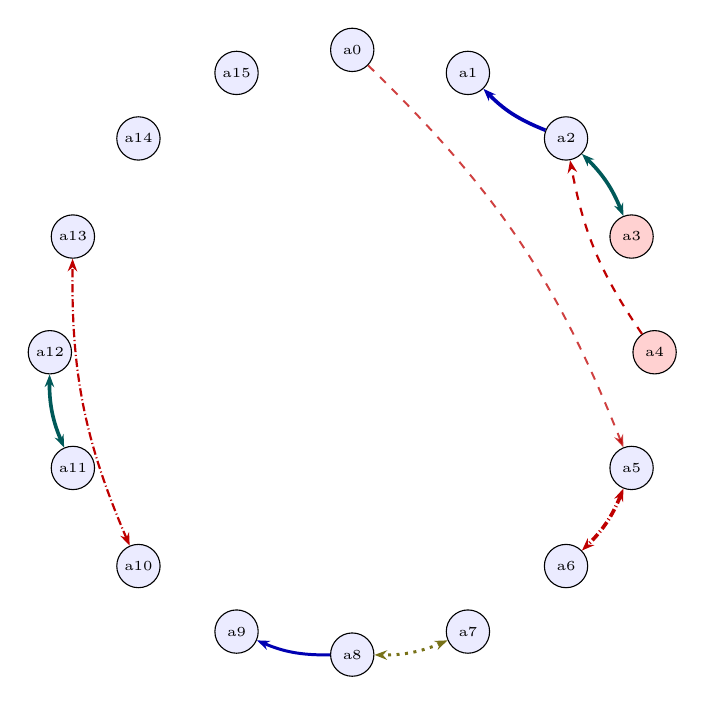
\begin{tikzpicture}[>={Stealth[length=1.6mm]}]
  \node[circle,draw,fill=blue!8,inner sep=1pt,minimum size=5.5mm,font=\tiny] (a0) at (90.0:3.84) {a0};
  \node[circle,draw,fill=blue!8,inner sep=1pt,minimum size=5.5mm,font=\tiny] (a1) at (67.5:3.84) {a1};
  \node[circle,draw,fill=blue!8,inner sep=1pt,minimum size=5.5mm,font=\tiny] (a2) at (45.0:3.84) {a2};
  \node[circle,draw,fill=red!18,inner sep=1pt,minimum size=5.5mm,font=\tiny] (a3) at (22.5:3.84) {a3};
  \node[circle,draw,fill=red!18,inner sep=1pt,minimum size=5.5mm,font=\tiny] (a4) at (0.0:3.84) {a4};
  \node[circle,draw,fill=blue!8,inner sep=1pt,minimum size=5.5mm,font=\tiny] (a5) at (-22.5:3.84) {a5};
  \node[circle,draw,fill=blue!8,inner sep=1pt,minimum size=5.5mm,font=\tiny] (a6) at (-45.0:3.84) {a6};
  \node[circle,draw,fill=blue!8,inner sep=1pt,minimum size=5.5mm,font=\tiny] (a7) at (-67.5:3.84) {a7};
  \node[circle,draw,fill=blue!8,inner sep=1pt,minimum size=5.5mm,font=\tiny] (a8) at (-90.0:3.84) {a8};
  \node[circle,draw,fill=blue!8,inner sep=1pt,minimum size=5.5mm,font=\tiny] (a9) at (-112.5:3.84) {a9};
  \node[circle,draw,fill=blue!8,inner sep=1pt,minimum size=5.5mm,font=\tiny] (a10) at (-135.0:3.84) {a10};
  \node[circle,draw,fill=blue!8,inner sep=1pt,minimum size=5.5mm,font=\tiny] (a11) at (-157.5:3.84) {a11};
  \node[circle,draw,fill=blue!8,inner sep=1pt,minimum size=5.5mm,font=\tiny] (a12) at (-180.0:3.84) {a12};
  \node[circle,draw,fill=blue!8,inner sep=1pt,minimum size=5.5mm,font=\tiny] (a13) at (-202.5:3.84) {a13};
  \node[circle,draw,fill=blue!8,inner sep=1pt,minimum size=5.5mm,font=\tiny] (a14) at (-225.0:3.84) {a14};
  \node[circle,draw,fill=blue!8,inner sep=1pt,minimum size=5.5mm,font=\tiny] (a15) at (-247.5:3.84) {a15};
  \draw[-{Stealth[length=1.6mm]}, blue!70!black, line width=1.31pt] (a2) to[bend left=12] (a1);
  \draw[{Stealth[length=1.6mm]}-{Stealth[length=1.6mm]}, teal!70!black, line width=1.31pt] (a2) to[bend left=12] (a3);
  \draw[-{Stealth[length=1.6mm]}, red!75!black, dashed, line width=0.79pt] (a4) to[bend left=12] (a2);
  \draw[{Stealth[length=1.6mm]}-{Stealth[length=1.6mm]}, red!75!black, densely dashdotted, line width=1.31pt] (a5) to[bend left=12] (a6);
  \draw[{Stealth[length=1.6mm]}-{Stealth[length=1.6mm]}, olive!80!black, dotted, line width=1.08pt] (a7) to[bend left=12] (a8);
  \draw[-{Stealth[length=1.6mm]}, blue!70!black, line width=1.08pt] (a8) to[bend left=12] (a9);
  \draw[{Stealth[length=1.6mm]}-{Stealth[length=1.6mm]}, teal!70!black, line width=1.31pt] (a11) to[bend left=12] (a12);
  \draw[-{Stealth[length=1.6mm]}, red!75!black, dashed, opacity=0.75, line width=0.71pt] (a0) to[bend left=12] (a5);
  \draw[{Stealth[length=1.6mm]}-{Stealth[length=1.6mm]}, red!75!black, densely dashdotted, line width=0.79pt] (a10) to[bend left=12] (a13);
\end{tikzpicture}
}
\\[2pt]{\footnotesize all gold edges: 9 factors}
\end{minipage}\hfill\begin{minipage}[t]{0.48\linewidth}\centering
\resizebox{!}{6.4cm}{%
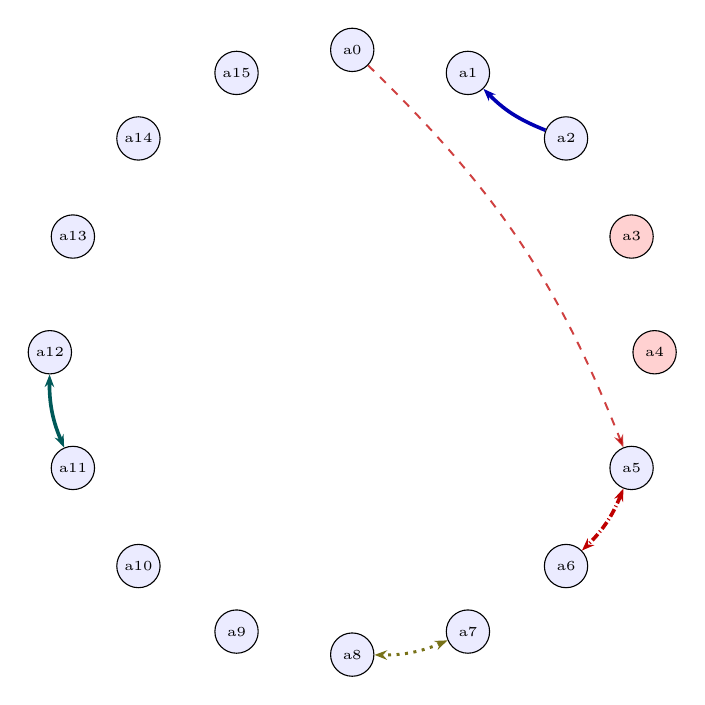
\begin{tikzpicture}[>={Stealth[length=1.6mm]}]
  \node[circle,draw,fill=blue!8,inner sep=1pt,minimum size=5.5mm,font=\tiny] (a0) at (90.0:3.84) {a0};
  \node[circle,draw,fill=blue!8,inner sep=1pt,minimum size=5.5mm,font=\tiny] (a1) at (67.5:3.84) {a1};
  \node[circle,draw,fill=blue!8,inner sep=1pt,minimum size=5.5mm,font=\tiny] (a2) at (45.0:3.84) {a2};
  \node[circle,draw,fill=red!18,inner sep=1pt,minimum size=5.5mm,font=\tiny] (a3) at (22.5:3.84) {a3};
  \node[circle,draw,fill=red!18,inner sep=1pt,minimum size=5.5mm,font=\tiny] (a4) at (0.0:3.84) {a4};
  \node[circle,draw,fill=blue!8,inner sep=1pt,minimum size=5.5mm,font=\tiny] (a5) at (-22.5:3.84) {a5};
  \node[circle,draw,fill=blue!8,inner sep=1pt,minimum size=5.5mm,font=\tiny] (a6) at (-45.0:3.84) {a6};
  \node[circle,draw,fill=blue!8,inner sep=1pt,minimum size=5.5mm,font=\tiny] (a7) at (-67.5:3.84) {a7};
  \node[circle,draw,fill=blue!8,inner sep=1pt,minimum size=5.5mm,font=\tiny] (a8) at (-90.0:3.84) {a8};
  \node[circle,draw,fill=blue!8,inner sep=1pt,minimum size=5.5mm,font=\tiny] (a9) at (-112.5:3.84) {a9};
  \node[circle,draw,fill=blue!8,inner sep=1pt,minimum size=5.5mm,font=\tiny] (a10) at (-135.0:3.84) {a10};
  \node[circle,draw,fill=blue!8,inner sep=1pt,minimum size=5.5mm,font=\tiny] (a11) at (-157.5:3.84) {a11};
  \node[circle,draw,fill=blue!8,inner sep=1pt,minimum size=5.5mm,font=\tiny] (a12) at (-180.0:3.84) {a12};
  \node[circle,draw,fill=blue!8,inner sep=1pt,minimum size=5.5mm,font=\tiny] (a13) at (-202.5:3.84) {a13};
  \node[circle,draw,fill=blue!8,inner sep=1pt,minimum size=5.5mm,font=\tiny] (a14) at (-225.0:3.84) {a14};
  \node[circle,draw,fill=blue!8,inner sep=1pt,minimum size=5.5mm,font=\tiny] (a15) at (-247.5:3.84) {a15};
  \draw[-{Stealth[length=1.6mm]}, blue!70!black, line width=1.31pt] (a2) to[bend left=12] (a1);
  \draw[{Stealth[length=1.6mm]}-{Stealth[length=1.6mm]}, red!75!black, densely dashdotted, line width=1.31pt] (a5) to[bend left=12] (a6);
  \draw[{Stealth[length=1.6mm]}-{Stealth[length=1.6mm]}, olive!80!black, dotted, line width=1.08pt] (a7) to[bend left=12] (a8);
  \draw[{Stealth[length=1.6mm]}-{Stealth[length=1.6mm]}, teal!70!black, line width=1.31pt] (a11) to[bend left=12] (a12);
  \draw[-{Stealth[length=1.6mm]}, red!75!black, dashed, opacity=0.75, line width=0.71pt] (a0) to[bend left=12] (a5);
\end{tikzpicture}
}
\\[2pt]{\footnotesize valid edges only: 5 factors}
\end{minipage}
\caption{Relation graph for \texttt{locobench-claude-5-fixed-f008-r1}. Nodes are atoms on a circle, tinted red when the item marks them non-factual (prior 0.1) and blue when factual (prior 0.9). Edges are gold relations: solid blue = entailment, dashed red = contradiction, double-headed teal = equivalence, dash-dotted red (double-headed) = exclusive (exactly-one), dotted olive (double-headed) = co-necessity (at-least-one); thickness scales with the factor probability. Ordering-only Precedence edges carry no factor and so are not drawn.}
\label{fig:graph-locobench-claude-5-fixed-f008-r1}
\end{figure}

\begin{table}[htbp]
\centering
\footnotesize
\setlength{\tabcolsep}{3.5pt}
\caption{The specific gold relations of \texttt{locobench-claude-5-fixed-f008-r1}. \textbf{$p$ used} is the factor probability the MRF received: the band midpoint, times $(1-\lambda)$ for a resolved concession, or \emph{none} for an ordering-only edge (no factor). \textbf{Valid} marks the deliberately-planted errors with their kind. \textbf{Res.} is the resolving atom of a resolved concession.}
\label{tab:rels-locobench-claude-5-fixed-f008-r1}
\begin{tabular}{lllllrll}
\toprule
ID & Endpoints & Sense & Coupling & Band & $p$ used & Valid & Res. \\
\midrule
\texttt{r000} & \texttt{a0} $\to$ \texttt{a1} & Precedence & \texttt{none} & moderate & \emph{none} & \checkmark &  \\
\texttt{r001} & \texttt{a2} $\to$ \texttt{a1} & Instantiation & \texttt{entailment} & strong & 0.925 & \checkmark &  \\
\texttt{r002} & \texttt{a2} $\leftrightarrow$ \texttt{a3} & Restatement & \texttt{equivalence} & strong & 0.925 & $\times$ {\scriptsize false\_endpoint} &  \\
\texttt{r003} & \texttt{a4} $\leftrightarrow$ \texttt{a2} & Contrast & \texttt{contradiction} & weak & 0.470 & $\times$ {\scriptsize false\_endpoint} &  \\
\texttt{r004} & \texttt{a5} $\leftrightarrow$ \texttt{a6} & Alternative & \texttt{exclusive} & strong & 0.925 & \checkmark &  \\
\texttt{r005} & \texttt{a7} $\leftrightarrow$ \texttt{a8} & Disjunction & \texttt{co\_necessity} & moderate & 0.720 & \checkmark &  \\
\texttt{r006} & \texttt{a8} $\to$ \texttt{a9} & Cause-Effect & \texttt{entailment} & moderate & 0.720 & $\times$ {\scriptsize wrong\_direction} &  \\
\texttt{r007} & \texttt{a11} $\leftrightarrow$ \texttt{a12} & Restatement & \texttt{equivalence} & strong & 0.925 & \checkmark &  \\
\texttt{r008} & \texttt{a0} $\to$ \texttt{a5} & Concession & \texttt{contradiction} & moderate & 0.396 & \checkmark & \texttt{a14} \\
\texttt{r009} & \texttt{a10} $\leftrightarrow$ \texttt{a13} & Alternative & \texttt{exclusive} & weak & 0.470 & $\times$ {\scriptsize wrong\_sense} &  \\
\bottomrule
\end{tabular}
\end{table}

\begin{table}[htbp]
\centering
\footnotesize
\caption{Atoms of \texttt{locobench-claude-5-fixed-f008-r1}: the \texttt{factual} label, the prior it maps to, the posterior marginal $P(a_i{=}1)$ the MRF returns, and the shift. Atoms dragged below their prior are the ones the coherence structure penalises.}
\label{tab:atoms-locobench-claude-5-fixed-f008-r1}
\begin{tabular}{llrrrp{7.2cm}}
\toprule
Atom & fact & $\pi_i$ & $P(a_i{=}1)$ & $\Delta$ & Text \\
\midrule
\texttt{a0} & \checkmark & 0.90 & 0.905 & +0.005 & \footnotesize Leadbeater and co-workers reported a transition-metal-free Suzuki-type coupling in 2003. \\
\texttt{a1} & \checkmark & 0.90 & 0.968 & +0.068 & \footnotesize Buchwald and co-workers measured palladium at parts-per-billion concentrations in commercial sodium carbonate. \\
\texttt{a2} & \checkmark & 0.90 & 0.745 & -0.155 & \footnotesize Inductively coupled plasma mass spectrometry detects trace metals in reagents at parts-per-billion levels. \\
\texttt{a3} & $\times$ & 0.10 & 0.433 & +0.333 & \footnotesize Combustion elemental analysis routinely quantifies metal contaminants at parts-per-billion concentrations. \\
\texttt{a4} & $\times$ & 0.10 & 0.103 & +0.003 & \footnotesize Thin-layer chromatography is the standard method for measuring trace metal content in inorganic bases. \\
\texttt{a5} & \checkmark & 0.90 & 0.715 & -0.185 & \footnotesize The sodium carbonate used in the coupling contained detectable palladium. \\
\texttt{a6} & \checkmark & 0.90 & 0.584 & -0.316 & \footnotesize The sodium carbonate used in the coupling was free of detectable palladium. \\
\texttt{a7} & \checkmark & 0.90 & 0.929 & +0.029 & \footnotesize The reagent bottle itself contained trace palladium as a manufacturing impurity. \\
\texttt{a8} & \checkmark & 0.90 & 0.947 & +0.047 & \footnotesize The stir bar used in the reaction carried residual palladium from earlier experiments. \\
\texttt{a9} & \checkmark & 0.90 & 0.955 & +0.055 & \footnotesize Palladium leaches from used Teflon-coated stir bars into subsequent reaction mixtures. \\
\texttt{a10} & \checkmark & 0.90 & 0.908 & +0.008 & \footnotesize Chemists repeat the synthesis with freshly purified starting materials to test whether the unexpected product persists. \\
\texttt{a11} & \checkmark & 0.90 & 0.979 & +0.079 & \footnotesize The unexpected product failed to form when ultrapure reagents were used. \\
\texttt{a12} & \checkmark & 0.90 & 0.979 & +0.079 & \footnotesize Use of reagents free of trace metals completely suppressed formation of the unexpected product. \\
\texttt{a13} & \checkmark & 0.90 & 0.908 & +0.008 & \footnotesize Spiking a reaction with a known quantity of a suspected contaminant tests whether it reproduces the unexpected product. \\
\texttt{a14} & \checkmark & 0.90 & 0.900 & +0.000 & \footnotesize The journal's editorial review board concluded that the reported metal-free coupling was catalysed by trace palladium contamination. \\
\texttt{a15} & \checkmark & 0.90 & 0.900 & +0.000 & \footnotesize The investigating committee ultimately determined that the unexpected product did not arise from a genuine new reaction pathway. \\
\bottomrule
\end{tabular}
\end{table}

\subsection{Computer Science -- base (\texttt{locobench-claude-5-fixed-f010-r1})}

\textbf{Topic:} Computer Science (Engineering \& Technology). \textbf{Family:} \texttt{f010} (CONFLICT), rung 1 (\emph{base}). \textbf{Scores:} mean-marg $= 0.783$, consist $= 0.485$, reified $= 0.254$, log-Z $= 0.315$.



\paragraph{Framing question.} \emph{How do investigators adjudicate between a defective code deployment and an underlying infrastructure fault when a large distributed system suffers a total outage and the two engineering teams submit irreconcilable post-incident accounts?}



\paragraph{Response.} {\small Adjudication between a defective deployment and a latent infrastructure fault begins not with the competing narratives but with the observable scope of the failure, because scope constrains which causal stories remain admissible. The Orion platform suffered a total service outage affecting all customer-facing endpoints; by contrast, the outage was confined to a single availability zone. Of these two characterizations, it is the platform-wide one that the instrumentation supports: load balancer logs recorded a simultaneous surge of health-check failures in every region, which indicates that no endpoint remained reachable and that the failure was global rather than localized. A fault whose signature appears everywhere at once is far more consistent with a change propagated through a shared control plane than with the degradation of any single hardware domain.

The second step is chronological reconstruction, which is where post-incident accounts are most often falsified. Investigators reconstructed the incident sequence from timestamped telemetry collected across all regions, even though the telemetry pipeline retained no log data from the period of the outage. What such a reconstruction yields is not an opinion about blame but an ordered record of state transitions against which each team's submission can be checked.

That record fixed the critical interval. The outage began four minutes after a configuration change was deployed to the routing tier, and this onset caused the deployed configuration to introduce an invalid routing rule into the request path. A four-minute lag is itself diagnostic, since it matches the propagation delay of routing state to edge nodes rather than the slower, uneven onset typical of storage or fabric saturation. Even so, the evidence does not license a single-fault conclusion. At least one of two defects was present in the cluster at the moment of failure — the invalid rule in the request path, or a misconfiguration of the cluster's underlying network fabric predating the deployment — and perhaps both were. Distinguishing a triggering change from a pre-existing condition that the change merely exposed is the substantive analytical problem, and it cannot be settled by scope data alone.

Pre-existing conditions of that kind also shape how each team frames its account. Specifically, the application engineering team attributed the outage to a failure of the shared storage backend, locating the defect below the layer it owned. The infrastructure team, despite that storage attribution, attributed the outage to the routing tier deployment, locating the defect above the layer it owned. Neither submission can be adjudicated by assertion, so investigators turned to intervention evidence. Rolling back the routing tier deployment restored service — a remediation that postdates the four-minute interval between the configuration change and the onset of the failure, and whose success therefore bears directly on the disputed link. On that basis the incident review board concluded that the routing tier deployment was the proximate cause of the outage, which settles the disagreement between the two teams: the storage backend cannot have been the proximate cause of a failure that a routing rollback terminated, and the fabric misconfiguration, real though it was, functioned as a background condition rather than the trigger.

A comparable adjudication was required for the question of data durability, where the record admits no middle ground. No customer transaction records were permanently lost during the outage; either that holds, or records for 12,000 customer transactions were permanently lost, and exactly one of these two accounts can be true. The durability finding entered the record in the first form — that is, the incident review board determined that no customer transaction records were permanently lost. Methodologically, this is the same discipline applied to causation: identify the mutually exclusive candidate states, locate the artifact that discriminates between them, and let the narratives submitted by the affected teams stand or fall against that artifact rather than against each other.}

\begin{figure}[htbp]
\centering
\begin{minipage}[t]{0.48\linewidth}\centering
\resizebox{!}{6.4cm}{%
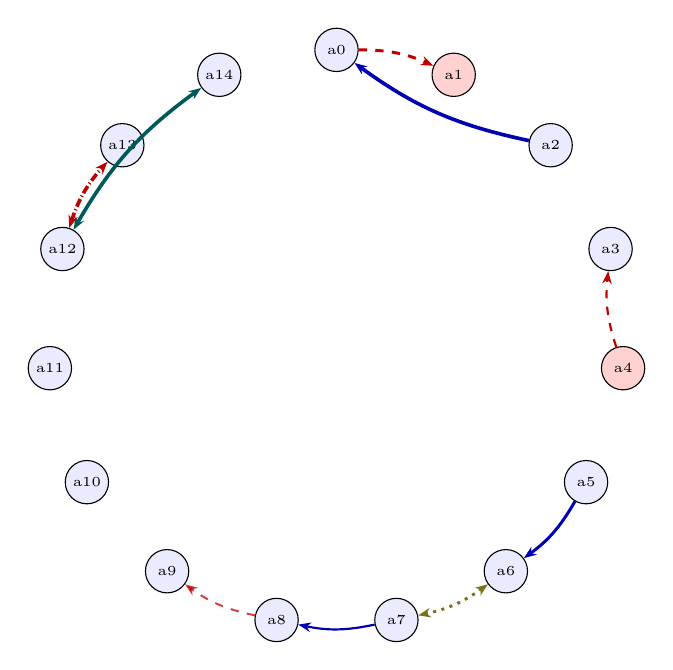
\begin{tikzpicture}[>={Stealth[length=1.6mm]}]
  \node[circle,draw,fill=blue!8,inner sep=1pt,minimum size=5.5mm,font=\tiny] (a0) at (90.0:3.66) {a0};
  \node[circle,draw,fill=red!18,inner sep=1pt,minimum size=5.5mm,font=\tiny] (a1) at (66.0:3.66) {a1};
  \node[circle,draw,fill=blue!8,inner sep=1pt,minimum size=5.5mm,font=\tiny] (a2) at (42.0:3.66) {a2};
  \node[circle,draw,fill=blue!8,inner sep=1pt,minimum size=5.5mm,font=\tiny] (a3) at (18.0:3.66) {a3};
  \node[circle,draw,fill=red!18,inner sep=1pt,minimum size=5.5mm,font=\tiny] (a4) at (-6.0:3.66) {a4};
  \node[circle,draw,fill=blue!8,inner sep=1pt,minimum size=5.5mm,font=\tiny] (a5) at (-30.0:3.66) {a5};
  \node[circle,draw,fill=blue!8,inner sep=1pt,minimum size=5.5mm,font=\tiny] (a6) at (-54.0:3.66) {a6};
  \node[circle,draw,fill=blue!8,inner sep=1pt,minimum size=5.5mm,font=\tiny] (a7) at (-78.0:3.66) {a7};
  \node[circle,draw,fill=blue!8,inner sep=1pt,minimum size=5.5mm,font=\tiny] (a8) at (-102.0:3.66) {a8};
  \node[circle,draw,fill=blue!8,inner sep=1pt,minimum size=5.5mm,font=\tiny] (a9) at (-126.0:3.66) {a9};
  \node[circle,draw,fill=blue!8,inner sep=1pt,minimum size=5.5mm,font=\tiny] (a10) at (-150.0:3.66) {a10};
  \node[circle,draw,fill=blue!8,inner sep=1pt,minimum size=5.5mm,font=\tiny] (a11) at (-174.0:3.66) {a11};
  \node[circle,draw,fill=blue!8,inner sep=1pt,minimum size=5.5mm,font=\tiny] (a12) at (-198.0:3.66) {a12};
  \node[circle,draw,fill=blue!8,inner sep=1pt,minimum size=5.5mm,font=\tiny] (a13) at (-222.0:3.66) {a13};
  \node[circle,draw,fill=blue!8,inner sep=1pt,minimum size=5.5mm,font=\tiny] (a14) at (-246.0:3.66) {a14};
  \draw[-{Stealth[length=1.6mm]}, blue!70!black, line width=1.31pt] (a2) to[bend left=12] (a0);
  \draw[-{Stealth[length=1.6mm]}, red!75!black, dashed, line width=1.08pt] (a0) to[bend left=12] (a1);
  \draw[-{Stealth[length=1.6mm]}, red!75!black, dashed, line width=0.79pt] (a4) to[bend left=12] (a3);
  \draw[-{Stealth[length=1.6mm]}, blue!70!black, line width=1.08pt] (a5) to[bend left=12] (a6);
  \draw[{Stealth[length=1.6mm]}-{Stealth[length=1.6mm]}, olive!80!black, dotted, line width=1.08pt] (a6) to[bend left=12] (a7);
  \draw[-{Stealth[length=1.6mm]}, blue!70!black, line width=0.79pt] (a7) to[bend left=12] (a8);
  \draw[-{Stealth[length=1.6mm]}, red!75!black, dashed, opacity=0.75, line width=0.71pt] (a8) to[bend left=12] (a9);
  \draw[{Stealth[length=1.6mm]}-{Stealth[length=1.6mm]}, red!75!black, densely dashdotted, line width=1.31pt] (a12) to[bend left=12] (a13);
  \draw[{Stealth[length=1.6mm]}-{Stealth[length=1.6mm]}, teal!70!black, line width=1.31pt] (a12) to[bend left=12] (a14);
\end{tikzpicture}
}
\\[2pt]{\footnotesize all gold edges: 9 factors}
\end{minipage}\hfill\begin{minipage}[t]{0.48\linewidth}\centering
\resizebox{!}{6.4cm}{%
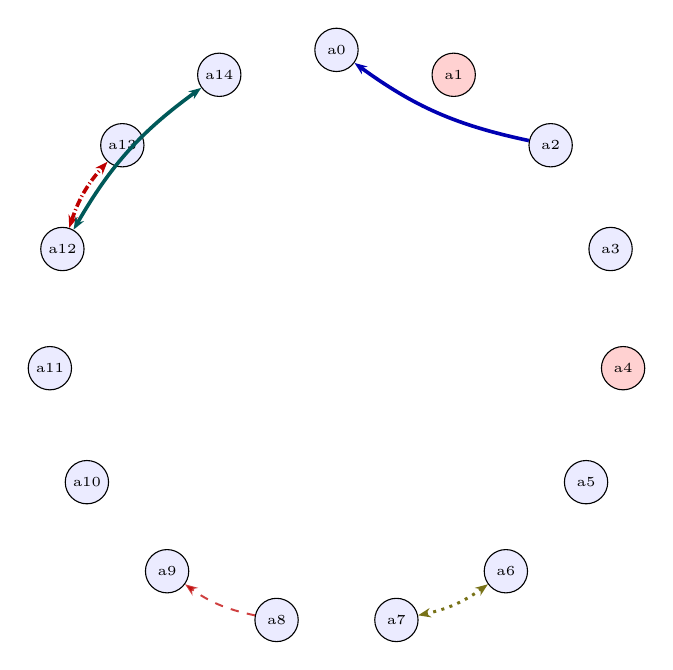
\begin{tikzpicture}[>={Stealth[length=1.6mm]}]
  \node[circle,draw,fill=blue!8,inner sep=1pt,minimum size=5.5mm,font=\tiny] (a0) at (90.0:3.66) {a0};
  \node[circle,draw,fill=red!18,inner sep=1pt,minimum size=5.5mm,font=\tiny] (a1) at (66.0:3.66) {a1};
  \node[circle,draw,fill=blue!8,inner sep=1pt,minimum size=5.5mm,font=\tiny] (a2) at (42.0:3.66) {a2};
  \node[circle,draw,fill=blue!8,inner sep=1pt,minimum size=5.5mm,font=\tiny] (a3) at (18.0:3.66) {a3};
  \node[circle,draw,fill=red!18,inner sep=1pt,minimum size=5.5mm,font=\tiny] (a4) at (-6.0:3.66) {a4};
  \node[circle,draw,fill=blue!8,inner sep=1pt,minimum size=5.5mm,font=\tiny] (a5) at (-30.0:3.66) {a5};
  \node[circle,draw,fill=blue!8,inner sep=1pt,minimum size=5.5mm,font=\tiny] (a6) at (-54.0:3.66) {a6};
  \node[circle,draw,fill=blue!8,inner sep=1pt,minimum size=5.5mm,font=\tiny] (a7) at (-78.0:3.66) {a7};
  \node[circle,draw,fill=blue!8,inner sep=1pt,minimum size=5.5mm,font=\tiny] (a8) at (-102.0:3.66) {a8};
  \node[circle,draw,fill=blue!8,inner sep=1pt,minimum size=5.5mm,font=\tiny] (a9) at (-126.0:3.66) {a9};
  \node[circle,draw,fill=blue!8,inner sep=1pt,minimum size=5.5mm,font=\tiny] (a10) at (-150.0:3.66) {a10};
  \node[circle,draw,fill=blue!8,inner sep=1pt,minimum size=5.5mm,font=\tiny] (a11) at (-174.0:3.66) {a11};
  \node[circle,draw,fill=blue!8,inner sep=1pt,minimum size=5.5mm,font=\tiny] (a12) at (-198.0:3.66) {a12};
  \node[circle,draw,fill=blue!8,inner sep=1pt,minimum size=5.5mm,font=\tiny] (a13) at (-222.0:3.66) {a13};
  \node[circle,draw,fill=blue!8,inner sep=1pt,minimum size=5.5mm,font=\tiny] (a14) at (-246.0:3.66) {a14};
  \draw[-{Stealth[length=1.6mm]}, blue!70!black, line width=1.31pt] (a2) to[bend left=12] (a0);
  \draw[{Stealth[length=1.6mm]}-{Stealth[length=1.6mm]}, olive!80!black, dotted, line width=1.08pt] (a6) to[bend left=12] (a7);
  \draw[-{Stealth[length=1.6mm]}, red!75!black, dashed, opacity=0.75, line width=0.71pt] (a8) to[bend left=12] (a9);
  \draw[{Stealth[length=1.6mm]}-{Stealth[length=1.6mm]}, red!75!black, densely dashdotted, line width=1.31pt] (a12) to[bend left=12] (a13);
  \draw[{Stealth[length=1.6mm]}-{Stealth[length=1.6mm]}, teal!70!black, line width=1.31pt] (a12) to[bend left=12] (a14);
\end{tikzpicture}
}
\\[2pt]{\footnotesize valid edges only: 5 factors}
\end{minipage}
\caption{Relation graph for \texttt{locobench-claude-5-fixed-f010-r1}. Nodes are atoms on a circle, tinted red when the item marks them non-factual (prior 0.1) and blue when factual (prior 0.9). Edges are gold relations: solid blue = entailment, dashed red = contradiction, double-headed teal = equivalence, dash-dotted red (double-headed) = exclusive (exactly-one), dotted olive (double-headed) = co-necessity (at-least-one); thickness scales with the factor probability. Ordering-only Precedence edges carry no factor and so are not drawn.}
\label{fig:graph-locobench-claude-5-fixed-f010-r1}
\end{figure}

\begin{table}[htbp]
\centering
\footnotesize
\setlength{\tabcolsep}{3.5pt}
\caption{The specific gold relations of \texttt{locobench-claude-5-fixed-f010-r1}. \textbf{$p$ used} is the factor probability the MRF received: the band midpoint, times $(1-\lambda)$ for a resolved concession, or \emph{none} for an ordering-only edge (no factor). \textbf{Valid} marks the deliberately-planted errors with their kind. \textbf{Res.} is the resolving atom of a resolved concession.}
\label{tab:rels-locobench-claude-5-fixed-f010-r1}
\begin{tabular}{lllllrll}
\toprule
ID & Endpoints & Sense & Coupling & Band & $p$ used & Valid & Res. \\
\midrule
\texttt{r000} & \texttt{a2} $\to$ \texttt{a0} & Evidence & \texttt{entailment} & strong & 0.925 & \checkmark &  \\
\texttt{r001} & \texttt{a0} $\leftrightarrow$ \texttt{a1} & Contrast & \texttt{contradiction} & moderate & 0.720 & $\times$ {\scriptsize false\_endpoint} &  \\
\texttt{r002} & \texttt{a4} $\to$ \texttt{a3} & Concession & \texttt{contradiction} & weak & 0.470 & $\times$ {\scriptsize false\_endpoint} &  \\
\texttt{r003} & \texttt{a5} $\to$ \texttt{a6} & Cause-Effect & \texttt{entailment} & moderate & 0.720 & $\times$ {\scriptsize wrong\_direction} &  \\
\texttt{r004} & \texttt{a6} $\leftrightarrow$ \texttt{a7} & Disjunction & \texttt{co\_necessity} & moderate & 0.720 & \checkmark &  \\
\texttt{r005} & \texttt{a7} $\to$ \texttt{a8} & Instantiation & \texttt{entailment} & weak & 0.470 & $\times$ {\scriptsize spurious} &  \\
\texttt{r006} & \texttt{a8} $\to$ \texttt{a9} & Concession & \texttt{contradiction} & moderate & 0.396 & \checkmark & \texttt{a11} \\
\texttt{r007} & \texttt{a5} $\to$ \texttt{a10} & Precedence & \texttt{none} & moderate & \emph{none} & \checkmark &  \\
\texttt{r008} & \texttt{a12} $\leftrightarrow$ \texttt{a13} & Alternative & \texttt{exclusive} & strong & 0.925 & \checkmark &  \\
\texttt{r009} & \texttt{a12} $\leftrightarrow$ \texttt{a14} & Restatement & \texttt{equivalence} & strong & 0.925 & \checkmark &  \\
\bottomrule
\end{tabular}
\end{table}

\begin{table}[htbp]
\centering
\footnotesize
\caption{Atoms of \texttt{locobench-claude-5-fixed-f010-r1}: the \texttt{factual} label, the prior it maps to, the posterior marginal $P(a_i{=}1)$ the MRF returns, and the shift. Atoms dragged below their prior are the ones the coherence structure penalises.}
\label{tab:atoms-locobench-claude-5-fixed-f010-r1}
\begin{tabular}{llrrrp{7.2cm}}
\toprule
Atom & fact & $\pi_i$ & $P(a_i{=}1)$ & $\Delta$ & Text \\
\midrule
\texttt{a0} & \checkmark & 0.90 & 0.989 & +0.089 & \footnotesize The Orion platform suffered a total service outage affecting all customer-facing endpoints. \\
\texttt{a1} & $\times$ & 0.10 & 0.042 & -0.058 & \footnotesize The outage was confined to a single availability zone. \\
\texttt{a2} & \checkmark & 0.90 & 0.939 & +0.039 & \footnotesize Load balancer logs recorded a simultaneous surge of health-check failures in every region. \\
\texttt{a3} & \checkmark & 0.90 & 0.901 & +0.001 & \footnotesize Investigators reconstructed the incident sequence from timestamped telemetry collected across all regions. \\
\texttt{a4} & $\times$ & 0.10 & 0.104 & +0.004 & \footnotesize The telemetry pipeline retained no log data from the period of the outage. \\
\texttt{a5} & \checkmark & 0.90 & 0.925 & +0.025 & \footnotesize The outage began four minutes after a configuration change was deployed to the routing tier. \\
\texttt{a6} & \checkmark & 0.90 & 0.968 & +0.068 & \footnotesize The deployed configuration introduced an invalid routing rule into the request path. \\
\texttt{a7} & \checkmark & 0.90 & 0.925 & +0.025 & \footnotesize The cluster's underlying network fabric was misconfigured before the deployment. \\
\texttt{a8} & \checkmark & 0.90 & 0.904 & +0.004 & \footnotesize The application engineering team attributed the outage to a failure of the shared storage backend. \\
\texttt{a9} & \checkmark & 0.90 & 0.929 & +0.029 & \footnotesize The infrastructure team attributed the outage to the routing tier deployment. \\
\texttt{a10} & \checkmark & 0.90 & 0.900 & +0.000 & \footnotesize Rolling back the routing tier deployment restored service. \\
\texttt{a11} & \checkmark & 0.90 & 0.900 & +0.000 & \footnotesize The incident review board concluded that the routing tier deployment was the proximate cause of the outage. \\
\texttt{a12} & \checkmark & 0.90 & 0.900 & +0.000 & \footnotesize No customer transaction records were permanently lost during the outage. \\
\texttt{a13} & \checkmark & 0.90 & 0.479 & -0.421 & \footnotesize Records for 12,000 customer transactions were permanently lost during the outage. \\
\texttt{a14} & \checkmark & 0.90 & 0.934 & +0.034 & \footnotesize The incident review board determined that no customer transaction records were permanently lost. \\
\bottomrule
\end{tabular}
\end{table}

\subsection{Culture -- shuffle\_block (\texttt{locobench-claude-5-fixed-f011-r1})}

\textbf{Topic:} Culture (Humanities). \textbf{Family:} \texttt{f011} (ORDER), rung 1 (\emph{shuffle\_block}). \textbf{Scores:} mean-marg $= 0.796$, consist $= 0.357$, reified $= 0.150$, log-Z $= 0.564$.



\paragraph{Framing question.} \emph{How do scholars adjudicate competing accounts of a cultural tradition's origin when one camp attributes it to independent invention within the community while the other traces it to borrowing from a neighboring society?}



\paragraph{Response.} {\small With priority established in the neighbor's favor, the analytic burden shifts from chronology to mechanism, since a demonstrated time lag identifies a direction of transfer without identifying its vehicle. At least one of two channels must have carried the tradition across the boundary, perhaps both: traders moving along the mountain route carried the practice into the community, or intermarriage between the two societies brought the practice into the community. Each channel leaves a distinct signature, the former in the distribution of trade goods along the route, the latter in kinship terminology and residence patterns. The traders' passage along the mountain route caused the review panel to conclude that the tradition entered the community by borrowing from the neighboring society.

The independent-invention hypothesis holds that similar traits can arise separately in societies without contact, and it draws its plausibility from the observation that comparable technical or ecological pressures often elicit comparable solutions. Where a trait is functionally advantageous, convergence is unremarkable and requires no historical connection at all. The decisive asymmetry between the two positions is thus chronological rather than functional. Establishing chronological priority requires showing that the trait appears earlier in the proposed donor society. Two mutually exclusive states of affairs are available, and exactly one of them must obtain: either the earliest securely dated evidence of the practice in the community predates the earliest securely dated evidence in the neighboring society, or the earliest securely dated evidence of the practice in the neighboring society is at least as old as any evidence of it in the community.

By contrast with that marital pathway, Franz Boas argued that shared arbitrary and nonfunctional details are stronger evidence of historical connection than shared function, on the reasoning that useful features may be reinvented anywhere, while gratuitous ones are unlikely to coincide twice. That criterion of arbitrary resemblance predates Clark Wissler's age-area hypothesis, which infers that the traits with the widest distribution are the oldest; equivalently, the hypothesis locates a trait's point of origin at the outer periphery of its distribution. Contemporary practice combines the two instruments rather than choosing between them: arbitrary formal detail identifies which resemblances are historically informative, distributional reasoning suggests a relative sequence, and absolute dating tests that sequence against an independent standard. Adjudication succeeds, then, not by weighing the intuitive appeal of invention against borrowing, but by determining which account survives the chronological and mechanistic tests that both are obliged to pass.

When two camps contend over the origin of a tradition, the dispute is resolved less by theoretical allegiance than by the differential predictions each position makes about the material and documentary record. Diffusionism explains shared cultural traits as the result of transmission between societies in contact, and an account of this kind therefore obliges its proponents to specify a route, an interval of contact, and a mechanism of transfer. That commitment makes the position falsifiable in a useful way: where no contact can be documented for the relevant period, the explanation collapses on its own terms, and the burden reverts to whoever proposed it.

Radiocarbon dating of associated organic material provides absolute dates for archaeological deposits, which confirms that the donor-priority requirement is an empirically decidable demand rather than a rhetorical one; in other words, radiocarbon yields calendar dates accurate to within a single year. Applied to the case at hand, the technique produced an outcome that initially seemed to cut both ways. Despite the first of those two possibilities — local priority for the community — the neighboring society's depictions of the motif are about three centuries older than the community's earliest depictions; that is, the motif appears in the neighboring society roughly 300 years before it appears in the community. The apparent contradiction was settled on procedural grounds when the journal's editorial board found that the independent-invention study had misdated its earliest samples, which removed the sole basis for local priority and left the donor sequence intact.}

\begin{figure}[htbp]
\centering
\begin{minipage}[t]{0.48\linewidth}\centering
\resizebox{!}{6.4cm}{%
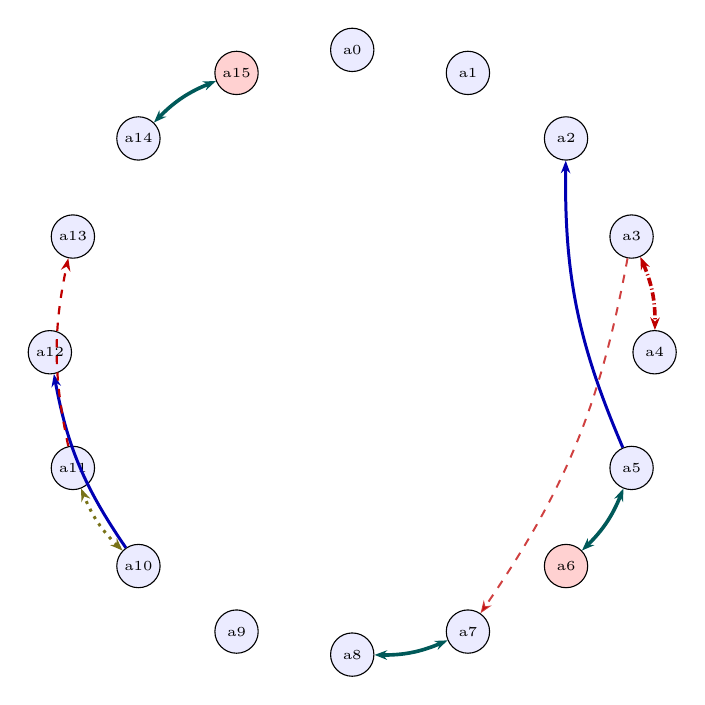
\begin{tikzpicture}[>={Stealth[length=1.6mm]}]
  \node[circle,draw,fill=blue!8,inner sep=1pt,minimum size=5.5mm,font=\tiny] (a0) at (90.0:3.84) {a0};
  \node[circle,draw,fill=blue!8,inner sep=1pt,minimum size=5.5mm,font=\tiny] (a1) at (67.5:3.84) {a1};
  \node[circle,draw,fill=blue!8,inner sep=1pt,minimum size=5.5mm,font=\tiny] (a2) at (45.0:3.84) {a2};
  \node[circle,draw,fill=blue!8,inner sep=1pt,minimum size=5.5mm,font=\tiny] (a3) at (22.5:3.84) {a3};
  \node[circle,draw,fill=blue!8,inner sep=1pt,minimum size=5.5mm,font=\tiny] (a4) at (0.0:3.84) {a4};
  \node[circle,draw,fill=blue!8,inner sep=1pt,minimum size=5.5mm,font=\tiny] (a5) at (-22.5:3.84) {a5};
  \node[circle,draw,fill=red!18,inner sep=1pt,minimum size=5.5mm,font=\tiny] (a6) at (-45.0:3.84) {a6};
  \node[circle,draw,fill=blue!8,inner sep=1pt,minimum size=5.5mm,font=\tiny] (a7) at (-67.5:3.84) {a7};
  \node[circle,draw,fill=blue!8,inner sep=1pt,minimum size=5.5mm,font=\tiny] (a8) at (-90.0:3.84) {a8};
  \node[circle,draw,fill=blue!8,inner sep=1pt,minimum size=5.5mm,font=\tiny] (a9) at (-112.5:3.84) {a9};
  \node[circle,draw,fill=blue!8,inner sep=1pt,minimum size=5.5mm,font=\tiny] (a10) at (-135.0:3.84) {a10};
  \node[circle,draw,fill=blue!8,inner sep=1pt,minimum size=5.5mm,font=\tiny] (a11) at (-157.5:3.84) {a11};
  \node[circle,draw,fill=blue!8,inner sep=1pt,minimum size=5.5mm,font=\tiny] (a12) at (-180.0:3.84) {a12};
  \node[circle,draw,fill=blue!8,inner sep=1pt,minimum size=5.5mm,font=\tiny] (a13) at (-202.5:3.84) {a13};
  \node[circle,draw,fill=blue!8,inner sep=1pt,minimum size=5.5mm,font=\tiny] (a14) at (-225.0:3.84) {a14};
  \node[circle,draw,fill=red!18,inner sep=1pt,minimum size=5.5mm,font=\tiny] (a15) at (-247.5:3.84) {a15};
  \draw[{Stealth[length=1.6mm]}-{Stealth[length=1.6mm]}, red!75!black, densely dashdotted, line width=1.31pt] (a3) to[bend left=12] (a4);
  \draw[-{Stealth[length=1.6mm]}, blue!70!black, line width=1.08pt] (a5) to[bend left=12] (a2);
  \draw[{Stealth[length=1.6mm]}-{Stealth[length=1.6mm]}, teal!70!black, line width=1.31pt] (a5) to[bend left=12] (a6);
  \draw[{Stealth[length=1.6mm]}-{Stealth[length=1.6mm]}, teal!70!black, line width=1.31pt] (a7) to[bend left=12] (a8);
  \draw[-{Stealth[length=1.6mm]}, red!75!black, dashed, opacity=0.75, line width=0.71pt] (a3) to[bend left=12] (a7);
  \draw[{Stealth[length=1.6mm]}-{Stealth[length=1.6mm]}, olive!80!black, dotted, line width=1.08pt] (a10) to[bend left=12] (a11);
  \draw[-{Stealth[length=1.6mm]}, blue!70!black, line width=1.08pt] (a10) to[bend left=12] (a12);
  \draw[-{Stealth[length=1.6mm]}, red!75!black, dashed, line width=0.79pt] (a11) to[bend left=12] (a13);
  \draw[{Stealth[length=1.6mm]}-{Stealth[length=1.6mm]}, teal!70!black, line width=1.31pt] (a14) to[bend left=12] (a15);
\end{tikzpicture}
}
\\[2pt]{\footnotesize all gold edges: 9 factors}
\end{minipage}\hfill\begin{minipage}[t]{0.48\linewidth}\centering
\resizebox{!}{6.4cm}{%
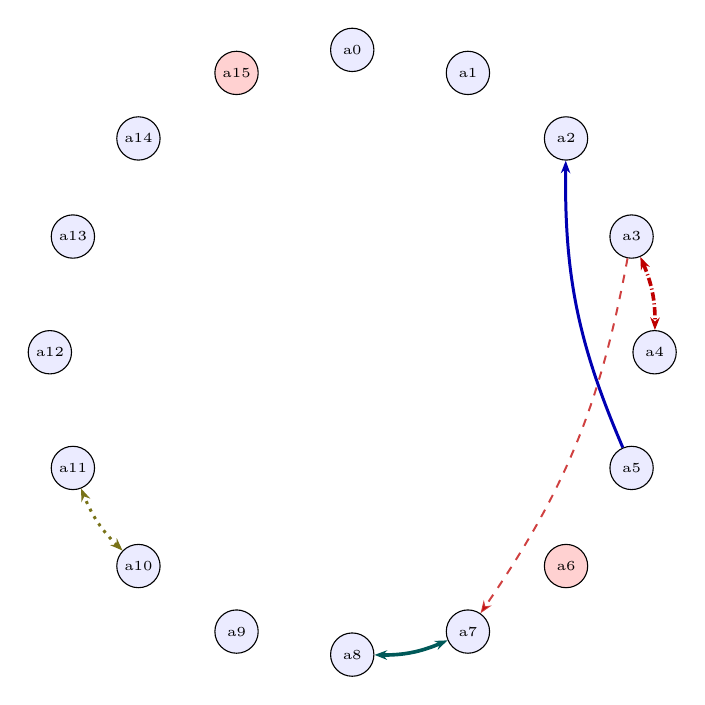
\begin{tikzpicture}[>={Stealth[length=1.6mm]}]
  \node[circle,draw,fill=blue!8,inner sep=1pt,minimum size=5.5mm,font=\tiny] (a0) at (90.0:3.84) {a0};
  \node[circle,draw,fill=blue!8,inner sep=1pt,minimum size=5.5mm,font=\tiny] (a1) at (67.5:3.84) {a1};
  \node[circle,draw,fill=blue!8,inner sep=1pt,minimum size=5.5mm,font=\tiny] (a2) at (45.0:3.84) {a2};
  \node[circle,draw,fill=blue!8,inner sep=1pt,minimum size=5.5mm,font=\tiny] (a3) at (22.5:3.84) {a3};
  \node[circle,draw,fill=blue!8,inner sep=1pt,minimum size=5.5mm,font=\tiny] (a4) at (0.0:3.84) {a4};
  \node[circle,draw,fill=blue!8,inner sep=1pt,minimum size=5.5mm,font=\tiny] (a5) at (-22.5:3.84) {a5};
  \node[circle,draw,fill=red!18,inner sep=1pt,minimum size=5.5mm,font=\tiny] (a6) at (-45.0:3.84) {a6};
  \node[circle,draw,fill=blue!8,inner sep=1pt,minimum size=5.5mm,font=\tiny] (a7) at (-67.5:3.84) {a7};
  \node[circle,draw,fill=blue!8,inner sep=1pt,minimum size=5.5mm,font=\tiny] (a8) at (-90.0:3.84) {a8};
  \node[circle,draw,fill=blue!8,inner sep=1pt,minimum size=5.5mm,font=\tiny] (a9) at (-112.5:3.84) {a9};
  \node[circle,draw,fill=blue!8,inner sep=1pt,minimum size=5.5mm,font=\tiny] (a10) at (-135.0:3.84) {a10};
  \node[circle,draw,fill=blue!8,inner sep=1pt,minimum size=5.5mm,font=\tiny] (a11) at (-157.5:3.84) {a11};
  \node[circle,draw,fill=blue!8,inner sep=1pt,minimum size=5.5mm,font=\tiny] (a12) at (-180.0:3.84) {a12};
  \node[circle,draw,fill=blue!8,inner sep=1pt,minimum size=5.5mm,font=\tiny] (a13) at (-202.5:3.84) {a13};
  \node[circle,draw,fill=blue!8,inner sep=1pt,minimum size=5.5mm,font=\tiny] (a14) at (-225.0:3.84) {a14};
  \node[circle,draw,fill=red!18,inner sep=1pt,minimum size=5.5mm,font=\tiny] (a15) at (-247.5:3.84) {a15};
  \draw[{Stealth[length=1.6mm]}-{Stealth[length=1.6mm]}, red!75!black, densely dashdotted, line width=1.31pt] (a3) to[bend left=12] (a4);
  \draw[-{Stealth[length=1.6mm]}, blue!70!black, line width=1.08pt] (a5) to[bend left=12] (a2);
  \draw[{Stealth[length=1.6mm]}-{Stealth[length=1.6mm]}, teal!70!black, line width=1.31pt] (a7) to[bend left=12] (a8);
  \draw[-{Stealth[length=1.6mm]}, red!75!black, dashed, opacity=0.75, line width=0.71pt] (a3) to[bend left=12] (a7);
  \draw[{Stealth[length=1.6mm]}-{Stealth[length=1.6mm]}, olive!80!black, dotted, line width=1.08pt] (a10) to[bend left=12] (a11);
\end{tikzpicture}
}
\\[2pt]{\footnotesize valid edges only: 5 factors}
\end{minipage}
\caption{Relation graph for \texttt{locobench-claude-5-fixed-f011-r1}. Nodes are atoms on a circle, tinted red when the item marks them non-factual (prior 0.1) and blue when factual (prior 0.9). Edges are gold relations: solid blue = entailment, dashed red = contradiction, double-headed teal = equivalence, dash-dotted red (double-headed) = exclusive (exactly-one), dotted olive (double-headed) = co-necessity (at-least-one); thickness scales with the factor probability. Ordering-only Precedence edges carry no factor and so are not drawn.}
\label{fig:graph-locobench-claude-5-fixed-f011-r1}
\end{figure}

\begin{table}[htbp]
\centering
\footnotesize
\setlength{\tabcolsep}{3.5pt}
\caption{The specific gold relations of \texttt{locobench-claude-5-fixed-f011-r1}. \textbf{$p$ used} is the factor probability the MRF received: the band midpoint, times $(1-\lambda)$ for a resolved concession, or \emph{none} for an ordering-only edge (no factor). \textbf{Valid} marks the deliberately-planted errors with their kind. \textbf{Res.} is the resolving atom of a resolved concession.}
\label{tab:rels-locobench-claude-5-fixed-f011-r1}
\begin{tabular}{lllllrll}
\toprule
ID & Endpoints & Sense & Coupling & Band & $p$ used & Valid & Res. \\
\midrule
\texttt{r000} & \texttt{a3} $\leftrightarrow$ \texttt{a4} & Alternative & \texttt{exclusive} & strong & 0.925 & \checkmark &  \\
\texttt{r001} & \texttt{a5} $\to$ \texttt{a2} & Evidence & \texttt{entailment} & moderate & 0.720 & \checkmark &  \\
\texttt{r002} & \texttt{a5} $\leftrightarrow$ \texttt{a6} & Restatement & \texttt{equivalence} & strong & 0.925 & $\times$ {\scriptsize false\_endpoint} &  \\
\texttt{r003} & \texttt{a7} $\leftrightarrow$ \texttt{a8} & Restatement & \texttt{equivalence} & strong & 0.925 & \checkmark &  \\
\texttt{r004} & \texttt{a3} $\to$ \texttt{a7} & Concession & \texttt{contradiction} & moderate & 0.396 & \checkmark & \texttt{a9} \\
\texttt{r005} & \texttt{a10} $\leftrightarrow$ \texttt{a11} & Disjunction & \texttt{co\_necessity} & moderate & 0.720 & \checkmark &  \\
\texttt{r006} & \texttt{a10} $\to$ \texttt{a12} & Cause-Effect & \texttt{entailment} & moderate & 0.720 & $\times$ {\scriptsize wrong\_sense} &  \\
\texttt{r007} & \texttt{a11} $\leftrightarrow$ \texttt{a13} & Contrast & \texttt{contradiction} & weak & 0.470 & $\times$ {\scriptsize spurious} &  \\
\texttt{r008} & \texttt{a13} $\to$ \texttt{a14} & Precedence & \texttt{none} & weak & \emph{none} & \checkmark &  \\
\texttt{r009} & \texttt{a14} $\leftrightarrow$ \texttt{a15} & Restatement & \texttt{equivalence} & strong & 0.925 & $\times$ {\scriptsize false\_endpoint} &  \\
\bottomrule
\end{tabular}
\end{table}

\begin{table}[htbp]
\centering
\footnotesize
\caption{Atoms of \texttt{locobench-claude-5-fixed-f011-r1}: the \texttt{factual} label, the prior it maps to, the posterior marginal $P(a_i{=}1)$ the MRF returns, and the shift. Atoms dragged below their prior are the ones the coherence structure penalises.}
\label{tab:atoms-locobench-claude-5-fixed-f011-r1}
\begin{tabular}{llrrrp{7.2cm}}
\toprule
Atom & fact & $\pi_i$ & $P(a_i{=}1)$ & $\Delta$ & Text \\
\midrule
\texttt{a0} & \checkmark & 0.90 & 0.900 & +0.000 & \footnotesize Diffusionism explains shared cultural traits as the result of transmission between societies in contact. \\
\texttt{a1} & \checkmark & 0.90 & 0.900 & +0.000 & \footnotesize The independent-invention hypothesis holds that similar traits can arise separately in societies without contact. \\
\texttt{a2} & \checkmark & 0.90 & 0.941 & +0.041 & \footnotesize Establishing chronological priority requires showing that the trait appears earlier in the proposed donor society. \\
\texttt{a3} & \checkmark & 0.90 & 0.673 & -0.227 & \footnotesize The earliest securely dated evidence of the practice in the community predates the earliest securely dated evidence in the neighboring society. \\
\texttt{a4} & \checkmark & 0.90 & 0.608 & -0.292 & \footnotesize The earliest securely dated evidence of the practice in the neighboring society is at least as old as any evidence of it in the community. \\
\texttt{a5} & \checkmark & 0.90 & 0.699 & -0.201 & \footnotesize Radiocarbon dating of associated organic material provides absolute dates for archaeological deposits. \\
\texttt{a6} & $\times$ & 0.10 & 0.407 & +0.307 & \footnotesize Radiocarbon dating yields calendar dates accurate to within a single year. \\
\texttt{a7} & \checkmark & 0.90 & 0.984 & +0.084 & \footnotesize The neighboring society's depictions of the motif are about three centuries older than the community's earliest depictions. \\
\texttt{a8} & \checkmark & 0.90 & 0.982 & +0.082 & \footnotesize The motif appears in the neighboring society roughly 300 years before it appears in the community. \\
\texttt{a9} & \checkmark & 0.90 & 0.900 & +0.000 & \footnotesize The journal's editorial board found that the independent-invention study had misdated its earliest samples. \\
\texttt{a10} & \checkmark & 0.90 & 0.947 & +0.047 & \footnotesize Traders moving along the mountain route carried the practice into the community. \\
\texttt{a11} & \checkmark & 0.90 & 0.932 & +0.032 & \footnotesize Intermarriage between the two societies brought the practice into the community. \\
\texttt{a12} & \checkmark & 0.90 & 0.955 & +0.055 & \footnotesize The review panel concluded that the tradition entered the community by borrowing from the neighboring society. \\
\texttt{a13} & \checkmark & 0.90 & 0.910 & +0.010 & \footnotesize Franz Boas argued that shared arbitrary and nonfunctional details are stronger evidence of historical connection than shared function. \\
\texttt{a14} & \checkmark & 0.90 & 0.632 & -0.268 & \footnotesize Clark Wissler's age-area hypothesis infers that the traits with the widest distribution are the oldest. \\
\texttt{a15} & $\times$ & 0.10 & 0.368 & +0.268 & \footnotesize Wissler's age-area hypothesis locates a trait's point of origin at the outer periphery of its distribution. \\
\bottomrule
\end{tabular}
\end{table}

\subsection{Education -- base (\texttt{locobench-claude-5-fixed-f014-r1})}

\textbf{Topic:} Education (Social Sciences). \textbf{Family:} \texttt{f014} (CONFLICT), rung 1 (\emph{base}). \textbf{Scores:} mean-marg $= 0.796$, consist $= 0.470$, reified $= 0.248$, log-Z $= 0.297$.



\paragraph{Framing question.} \emph{How do researchers adjudicate between the competing explanations that a school's rising test scores reflect genuine instructional improvement or merely changes in which students were tested?}



\paragraph{Response.} {\small The competing explanations differ in what they claim about students, not about schools, and the adjudication turns on that distinction. Aggregate mean test scores at a school can rise without any individual student's performance improving, since a mean is a property of whoever happens to sit the exam: drop the lowest scorers from the tested pool, or replace them with stronger entrants, and the average climbs while every remaining child performs exactly as before. Because a school-level average is vulnerable in this way, researchers link individual student records across years, which allows them to separate within-student growth from changes in who was tested. The linkage converts an ambiguous aggregate into two distinct quantities, only one of which can be credited to instruction.

In the case at issue, the analysts followed the same students across successive years rather than comparing successive grade cohorts. Equivalently, the analysis relied on longitudinal individual-level student tracking instead of cross-sectional cohort comparisons, so that a third-grade class in one year was not silently treated as the counterpart of a different third-grade class in the next. Whereas that separation of genuine growth from compositional churn depends on records tied to identifiable pupils over time, value-added models can be estimated without student-level identifiers that link records across years. Federal accountability rules constrain the composition question directly: No Child Left Behind required schools to test at least 95 percent of enrolled students for accountability purposes, a floor designed precisely to limit how much of a reported average a school could manufacture by selective omission.

Two descriptions of this school's compliance were in circulation, and they cannot both hold, though one of them must: either the school's test participation rate remained above 95 percent in every year of the study period, or that rate fell below 95 percent in at least one year. The state auditor determined that participation fell below the 95 percent threshold in two of the four years examined, which establishes the second description and thereby licenses a compositional reading of the score trend. Once documented shortfalls in participation are on the record, the burden shifts to the instructional account, which must explain why gains appeared in precisely the years when fewer enrolled students were assessed.

The arithmetic of exclusion is not in dispute. Excluding students with disabilities from the tested population raises a school's reported average score, because the omitted scores lie disproportionately in the lower tail of the distribution. On the other hand, a school's mean score is unaffected by which students are excluded as long as the exclusion rate stays below 10 percent, so the magnitude of any omission, and not merely its existence, governs how much of an apparent gain it can explain.

The classification records supply the decisive detail. The share of the school's students classified for alternate assessment rose from 8 percent to 17 percent over the study period, and that rise is indicated by the reclassification of low-scoring students into testing-exempt categories before the exam. At least one of two removal mechanisms was operating, and perhaps both: that reclassification of low scorers into exempt status, or the transfer of low-scoring students out of the school before the exam was administered. Although that doubling of the alternate-assessment share was on the books, the district attributed the score increase to a new phonics-based reading curriculum introduced in the second year; that attribution preceded the state audit board's conclusion that the reported score gains reflected the exclusion of low-performing students from testing rather than the new curriculum. The board's finding resolves the apparent standoff between the classification pattern and the district's explanation, assigning the observed improvement to a shrinking tested population rather than to instruction, and it illustrates why participation and classification data are indispensable companions to any score series.}

\begin{figure}[htbp]
\centering
\begin{minipage}[t]{0.48\linewidth}\centering
\resizebox{!}{6.4cm}{%
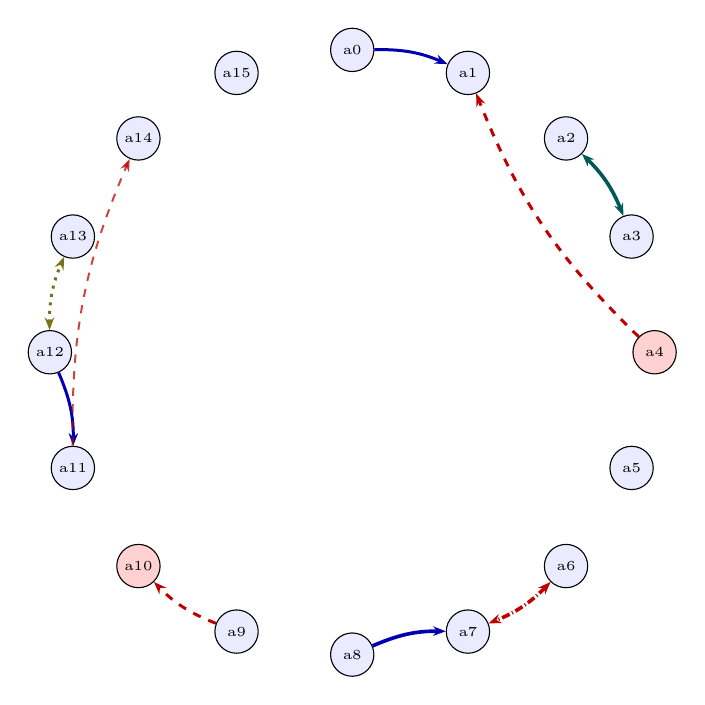
\begin{tikzpicture}[>={Stealth[length=1.6mm]}]
  \node[circle,draw,fill=blue!8,inner sep=1pt,minimum size=5.5mm,font=\tiny] (a0) at (90.0:3.84) {a0};
  \node[circle,draw,fill=blue!8,inner sep=1pt,minimum size=5.5mm,font=\tiny] (a1) at (67.5:3.84) {a1};
  \node[circle,draw,fill=blue!8,inner sep=1pt,minimum size=5.5mm,font=\tiny] (a2) at (45.0:3.84) {a2};
  \node[circle,draw,fill=blue!8,inner sep=1pt,minimum size=5.5mm,font=\tiny] (a3) at (22.5:3.84) {a3};
  \node[circle,draw,fill=red!18,inner sep=1pt,minimum size=5.5mm,font=\tiny] (a4) at (0.0:3.84) {a4};
  \node[circle,draw,fill=blue!8,inner sep=1pt,minimum size=5.5mm,font=\tiny] (a5) at (-22.5:3.84) {a5};
  \node[circle,draw,fill=blue!8,inner sep=1pt,minimum size=5.5mm,font=\tiny] (a6) at (-45.0:3.84) {a6};
  \node[circle,draw,fill=blue!8,inner sep=1pt,minimum size=5.5mm,font=\tiny] (a7) at (-67.5:3.84) {a7};
  \node[circle,draw,fill=blue!8,inner sep=1pt,minimum size=5.5mm,font=\tiny] (a8) at (-90.0:3.84) {a8};
  \node[circle,draw,fill=blue!8,inner sep=1pt,minimum size=5.5mm,font=\tiny] (a9) at (-112.5:3.84) {a9};
  \node[circle,draw,fill=red!18,inner sep=1pt,minimum size=5.5mm,font=\tiny] (a10) at (-135.0:3.84) {a10};
  \node[circle,draw,fill=blue!8,inner sep=1pt,minimum size=5.5mm,font=\tiny] (a11) at (-157.5:3.84) {a11};
  \node[circle,draw,fill=blue!8,inner sep=1pt,minimum size=5.5mm,font=\tiny] (a12) at (-180.0:3.84) {a12};
  \node[circle,draw,fill=blue!8,inner sep=1pt,minimum size=5.5mm,font=\tiny] (a13) at (-202.5:3.84) {a13};
  \node[circle,draw,fill=blue!8,inner sep=1pt,minimum size=5.5mm,font=\tiny] (a14) at (-225.0:3.84) {a14};
  \node[circle,draw,fill=blue!8,inner sep=1pt,minimum size=5.5mm,font=\tiny] (a15) at (-247.5:3.84) {a15};
  \draw[-{Stealth[length=1.6mm]}, blue!70!black, line width=1.08pt] (a0) to[bend left=12] (a1);
  \draw[{Stealth[length=1.6mm]}-{Stealth[length=1.6mm]}, teal!70!black, line width=1.31pt] (a2) to[bend left=12] (a3);
  \draw[-{Stealth[length=1.6mm]}, red!75!black, dashed, line width=1.08pt] (a4) to[bend left=12] (a1);
  \draw[{Stealth[length=1.6mm]}-{Stealth[length=1.6mm]}, red!75!black, densely dashdotted, line width=1.31pt] (a6) to[bend left=12] (a7);
  \draw[-{Stealth[length=1.6mm]}, blue!70!black, line width=1.31pt] (a8) to[bend left=12] (a7);
  \draw[-{Stealth[length=1.6mm]}, red!75!black, dashed, line width=1.08pt] (a9) to[bend left=12] (a10);
  \draw[-{Stealth[length=1.6mm]}, blue!70!black, line width=1.08pt] (a12) to[bend left=12] (a11);
  \draw[{Stealth[length=1.6mm]}-{Stealth[length=1.6mm]}, olive!80!black, dotted, line width=1.08pt] (a12) to[bend left=12] (a13);
  \draw[-{Stealth[length=1.6mm]}, red!75!black, dashed, opacity=0.75, line width=0.71pt] (a11) to[bend left=12] (a14);
\end{tikzpicture}
}
\\[2pt]{\footnotesize all gold edges: 9 factors}
\end{minipage}\hfill\begin{minipage}[t]{0.48\linewidth}\centering
\resizebox{!}{6.4cm}{%
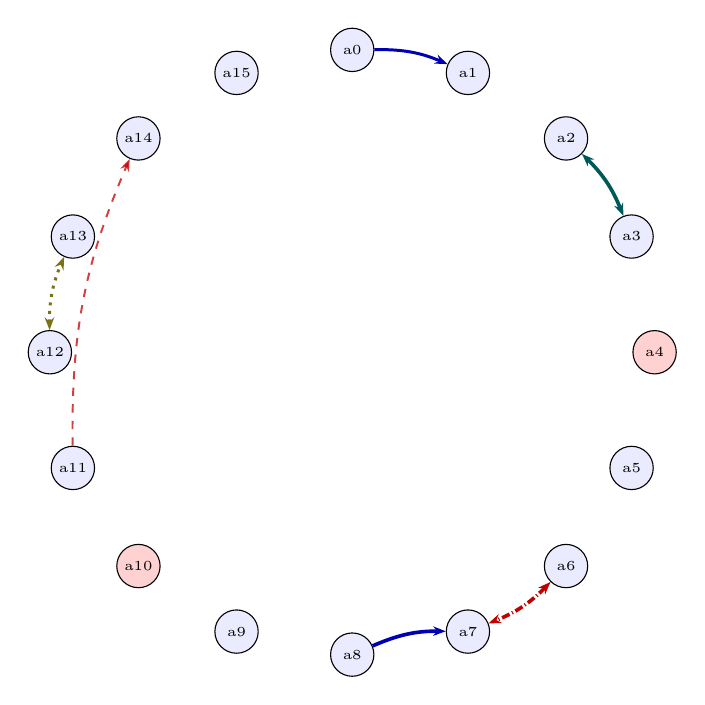
\begin{tikzpicture}[>={Stealth[length=1.6mm]}]
  \node[circle,draw,fill=blue!8,inner sep=1pt,minimum size=5.5mm,font=\tiny] (a0) at (90.0:3.84) {a0};
  \node[circle,draw,fill=blue!8,inner sep=1pt,minimum size=5.5mm,font=\tiny] (a1) at (67.5:3.84) {a1};
  \node[circle,draw,fill=blue!8,inner sep=1pt,minimum size=5.5mm,font=\tiny] (a2) at (45.0:3.84) {a2};
  \node[circle,draw,fill=blue!8,inner sep=1pt,minimum size=5.5mm,font=\tiny] (a3) at (22.5:3.84) {a3};
  \node[circle,draw,fill=red!18,inner sep=1pt,minimum size=5.5mm,font=\tiny] (a4) at (0.0:3.84) {a4};
  \node[circle,draw,fill=blue!8,inner sep=1pt,minimum size=5.5mm,font=\tiny] (a5) at (-22.5:3.84) {a5};
  \node[circle,draw,fill=blue!8,inner sep=1pt,minimum size=5.5mm,font=\tiny] (a6) at (-45.0:3.84) {a6};
  \node[circle,draw,fill=blue!8,inner sep=1pt,minimum size=5.5mm,font=\tiny] (a7) at (-67.5:3.84) {a7};
  \node[circle,draw,fill=blue!8,inner sep=1pt,minimum size=5.5mm,font=\tiny] (a8) at (-90.0:3.84) {a8};
  \node[circle,draw,fill=blue!8,inner sep=1pt,minimum size=5.5mm,font=\tiny] (a9) at (-112.5:3.84) {a9};
  \node[circle,draw,fill=red!18,inner sep=1pt,minimum size=5.5mm,font=\tiny] (a10) at (-135.0:3.84) {a10};
  \node[circle,draw,fill=blue!8,inner sep=1pt,minimum size=5.5mm,font=\tiny] (a11) at (-157.5:3.84) {a11};
  \node[circle,draw,fill=blue!8,inner sep=1pt,minimum size=5.5mm,font=\tiny] (a12) at (-180.0:3.84) {a12};
  \node[circle,draw,fill=blue!8,inner sep=1pt,minimum size=5.5mm,font=\tiny] (a13) at (-202.5:3.84) {a13};
  \node[circle,draw,fill=blue!8,inner sep=1pt,minimum size=5.5mm,font=\tiny] (a14) at (-225.0:3.84) {a14};
  \node[circle,draw,fill=blue!8,inner sep=1pt,minimum size=5.5mm,font=\tiny] (a15) at (-247.5:3.84) {a15};
  \draw[-{Stealth[length=1.6mm]}, blue!70!black, line width=1.08pt] (a0) to[bend left=12] (a1);
  \draw[{Stealth[length=1.6mm]}-{Stealth[length=1.6mm]}, teal!70!black, line width=1.31pt] (a2) to[bend left=12] (a3);
  \draw[{Stealth[length=1.6mm]}-{Stealth[length=1.6mm]}, red!75!black, densely dashdotted, line width=1.31pt] (a6) to[bend left=12] (a7);
  \draw[-{Stealth[length=1.6mm]}, blue!70!black, line width=1.31pt] (a8) to[bend left=12] (a7);
  \draw[{Stealth[length=1.6mm]}-{Stealth[length=1.6mm]}, olive!80!black, dotted, line width=1.08pt] (a12) to[bend left=12] (a13);
  \draw[-{Stealth[length=1.6mm]}, red!75!black, dashed, opacity=0.75, line width=0.71pt] (a11) to[bend left=12] (a14);
\end{tikzpicture}
}
\\[2pt]{\footnotesize valid edges only: 6 factors}
\end{minipage}
\caption{Relation graph for \texttt{locobench-claude-5-fixed-f014-r1}. Nodes are atoms on a circle, tinted red when the item marks them non-factual (prior 0.1) and blue when factual (prior 0.9). Edges are gold relations: solid blue = entailment, dashed red = contradiction, double-headed teal = equivalence, dash-dotted red (double-headed) = exclusive (exactly-one), dotted olive (double-headed) = co-necessity (at-least-one); thickness scales with the factor probability. Ordering-only Precedence edges carry no factor and so are not drawn.}
\label{fig:graph-locobench-claude-5-fixed-f014-r1}
\end{figure}

\begin{table}[htbp]
\centering
\footnotesize
\setlength{\tabcolsep}{3.5pt}
\caption{The specific gold relations of \texttt{locobench-claude-5-fixed-f014-r1}. \textbf{$p$ used} is the factor probability the MRF received: the band midpoint, times $(1-\lambda)$ for a resolved concession, or \emph{none} for an ordering-only edge (no factor). \textbf{Valid} marks the deliberately-planted errors with their kind. \textbf{Res.} is the resolving atom of a resolved concession.}
\label{tab:rels-locobench-claude-5-fixed-f014-r1}
\begin{tabular}{lllllrll}
\toprule
ID & Endpoints & Sense & Coupling & Band & $p$ used & Valid & Res. \\
\midrule
\texttt{r000} & \texttt{a0} $\to$ \texttt{a1} & Cause-Effect & \texttt{entailment} & moderate & 0.720 & \checkmark &  \\
\texttt{r001} & \texttt{a2} $\leftrightarrow$ \texttt{a3} & Restatement & \texttt{equivalence} & strong & 0.925 & \checkmark &  \\
\texttt{r002} & \texttt{a4} $\leftrightarrow$ \texttt{a1} & Contrast & \texttt{contradiction} & moderate & 0.720 & $\times$ {\scriptsize false\_endpoint} &  \\
\texttt{r003} & \texttt{a6} $\leftrightarrow$ \texttt{a7} & Alternative & \texttt{exclusive} & strong & 0.925 & \checkmark &  \\
\texttt{r004} & \texttt{a8} $\to$ \texttt{a7} & Evidence & \texttt{entailment} & strong & 0.925 & \checkmark &  \\
\texttt{r005} & \texttt{a9} $\leftrightarrow$ \texttt{a10} & Contrast & \texttt{contradiction} & moderate & 0.720 & $\times$ {\scriptsize false\_endpoint} &  \\
\texttt{r006} & \texttt{a12} $\to$ \texttt{a11} & Evidence & \texttt{entailment} & moderate & 0.720 & $\times$ {\scriptsize wrong\_direction} &  \\
\texttt{r007} & \texttt{a12} $\leftrightarrow$ \texttt{a13} & Disjunction & \texttt{co\_necessity} & moderate & 0.720 & \checkmark &  \\
\texttt{r008} & \texttt{a11} $\to$ \texttt{a14} & Concession & \texttt{contradiction} & moderate & 0.396 & \checkmark & \texttt{a15} \\
\texttt{r009} & \texttt{a14} $\to$ \texttt{a15} & Precedence & \texttt{none} & weak & \emph{none} & $\times$ {\scriptsize wrong\_sense} &  \\
\bottomrule
\end{tabular}
\end{table}

\begin{table}[htbp]
\centering
\footnotesize
\caption{Atoms of \texttt{locobench-claude-5-fixed-f014-r1}: the \texttt{factual} label, the prior it maps to, the posterior marginal $P(a_i{=}1)$ the MRF returns, and the shift. Atoms dragged below their prior are the ones the coherence structure penalises.}
\label{tab:atoms-locobench-claude-5-fixed-f014-r1}
\begin{tabular}{llrrrp{7.2cm}}
\toprule
Atom & fact & $\pi_i$ & $P(a_i{=}1)$ & $\Delta$ & Text \\
\midrule
\texttt{a0} & \checkmark & 0.90 & 0.924 & +0.024 & \footnotesize Aggregate mean test scores at a school can rise without any individual student's performance improving. \\
\texttt{a1} & \checkmark & 0.90 & 0.950 & +0.050 & \footnotesize Researchers link individual student records across years to separate within-student growth from changes in who was tested. \\
\texttt{a2} & \checkmark & 0.90 & 0.979 & +0.079 & \footnotesize The researchers followed the same students across successive years rather than comparing successive grade cohorts. \\
\texttt{a3} & \checkmark & 0.90 & 0.979 & +0.079 & \footnotesize The analysis relied on longitudinal individual-level student tracking instead of cross-sectional cohort comparisons. \\
\texttt{a4} & $\times$ & 0.10 & 0.063 & -0.037 & \footnotesize Value-added models can be estimated without student-level identifiers that link records across years. \\
\texttt{a5} & \checkmark & 0.90 & 0.900 & +0.000 & \footnotesize No Child Left Behind required schools to test at least 95 percent of enrolled students for accountability purposes. \\
\texttt{a6} & \checkmark & 0.90 & 0.463 & -0.437 & \footnotesize The school's test participation rate remained above 95 percent in every year of the study period. \\
\texttt{a7} & \checkmark & 0.90 & 0.928 & +0.028 & \footnotesize The school's test participation rate fell below 95 percent in at least one year of the study period. \\
\texttt{a8} & \checkmark & 0.90 & 0.917 & +0.017 & \footnotesize The state auditor determined that participation fell below the 95 percent threshold in two of the four years examined. \\
\texttt{a9} & \checkmark & 0.90 & 0.924 & +0.024 & \footnotesize Excluding students with disabilities from the tested population raises a school's reported average score. \\
\texttt{a10} & $\times$ & 0.10 & 0.046 & -0.054 & \footnotesize A school's mean score is unaffected by which students are excluded as long as the exclusion rate stays below 10 percent. \\
\texttt{a11} & \checkmark & 0.90 & 0.962 & +0.062 & \footnotesize The share of the school's students classified for alternate assessment rose from 8 percent to 17 percent over the study period. \\
\texttt{a12} & \checkmark & 0.90 & 0.947 & +0.047 & \footnotesize Low-scoring students were reclassified into testing-exempt categories before the exam. \\
\texttt{a13} & \checkmark & 0.90 & 0.929 & +0.029 & \footnotesize Low-scoring students transferred out of the school before the exam was administered. \\
\texttt{a14} & \checkmark & 0.90 & 0.931 & +0.031 & \footnotesize The district attributed the score increase to a new phonics-based reading curriculum introduced in the second year. \\
\texttt{a15} & \checkmark & 0.90 & 0.900 & +0.000 & \footnotesize The state audit board concluded that the reported score gains reflected the exclusion of low-performing students from testing rather than the new curriculum. \\
\bottomrule
\end{tabular}
\end{table}

\subsection{Biology -- base (\texttt{locobench-claude-5-fixed-f006-r1})}

\textbf{Topic:} Biology (Natural Sciences). \textbf{Family:} \texttt{f006} (CONFLICT), rung 1 (\emph{base}). \textbf{Scores:} mean-marg $= 0.783$, consist $= 0.454$, reified $= 0.239$, log-Z $= 0.370$.



\paragraph{Framing question.} \emph{How do researchers establish whether a mass extinction event was driven by an extraterrestrial impact or by prolonged volcanic activity, and what evidence settles the matter for a particular episode in the fossil record?}



\paragraph{Response.} {\small Distinguishing an impact from a volcanic driver of a mass extinction rests on markers preserved in the boundary interval itself, and on whether the ages of the candidate mechanism and the biotic turnover coincide. The most influential such marker was announced in 1980, when Luis Alvarez and colleagues first reported the iridium anomaly at the Cretaceous–Paleogene boundary; that report indicates that the boundary layer is enriched in iridium relative to the surrounding strata. The question admits no middle ground: either the boundary clay carries an excess of that element, or it shows no iridium enrichment relative to the surrounding strata, and one of these two descriptions must hold while the other fails. The geochemical background against which any such measurement is interpreted therefore matters, and iridium is more abundant in Earth's continental crust than in chondritic meteorites; the boundary layer's enrichment, by contrast, has been read as a signal foreign to ordinary sedimentary sources.

A second diagnostic is microstructural rather than geochemical. Shocked quartz forms only at the shock pressures generated by hypervelocity impacts, which makes its presence in a stratigraphic horizon difficult to attribute to eruptive processes; on the other hand, shocked quartz forms at shock pressures below 0.5 gigapascals. The distribution of these grains is as important as their existence, because a local disturbance would produce only a local signal. Shocked quartz grains occur in Cretaceous–Paleogene boundary sediments at sites on multiple continents, and that intercontinental spread indicates that the Chicxulub crater lies buried beneath the Yucatán Peninsula in Mexico.

Identifying a candidate structure is only the beginning of the argument, since a crater must be sized and dated before it can be tied to a horizon in the fossil record. Gravity and magnetic surveys, supplemented by drill cores through the Yucatán platform, define the concentric ring structure and its outer rim. The buried structure measures roughly 180 kilometres across, and because it spans that distance, argon–argon dating of impact glass places the Chicxulub event at about 66 million years ago.

Chronological agreement between mechanism and extinction is what converts correlation into a causal case, and it requires that both the event and the biotic turnover be dated within the resolution of the available radiometric and biostratigraphic methods. The Cretaceous–Paleogene boundary is dated to approximately 66 million years ago; equivalently, the end-Cretaceous mass extinction took place roughly 66 million years before the present. Coincidence at this level of precision is a necessary but not a sufficient condition, since a long-lived volcanic province can also overlap a boundary within the same error envelope.

The competing mechanisms are usually evaluated through their atmospheric consequences. At least one of the following was operating in the latest Cretaceous, and perhaps both: the Chicxulub impact lofted sulfate aerosols and dust that abruptly darkened and cooled the global atmosphere, and Deccan Traps eruptions injected large volumes of sulfur dioxide and carbon dioxide into the atmosphere before the boundary. Despite that pre-boundary loading of the atmosphere with volcanic gases, a 2010 review panel of 41 scientists concluded that the Chicxulub impact triggered the end-Cretaceous mass extinction. The apparent tension between the two atmospheric forcings is settled by a further finding of the same review, which determined that Deccan Traps volcanism was not the principal cause of the end-Cretaceous extinction; the eruptions thus figure as a background stress rather than as the proximate agent of the crisis. It is worth noting the sequence in which the two assessments entered the literature: the original report of the boundary iridium anomaly by Alvarez and colleagues postdates that panel's verdict on Chicxulub. For this episode, then, the geochemical anomaly, the globally distributed shocked quartz, the buried crater, and the concordance of ages together settle the matter in favour of impact.}

\begin{figure}[htbp]
\centering
\begin{minipage}[t]{0.48\linewidth}\centering
\resizebox{!}{6.4cm}{%
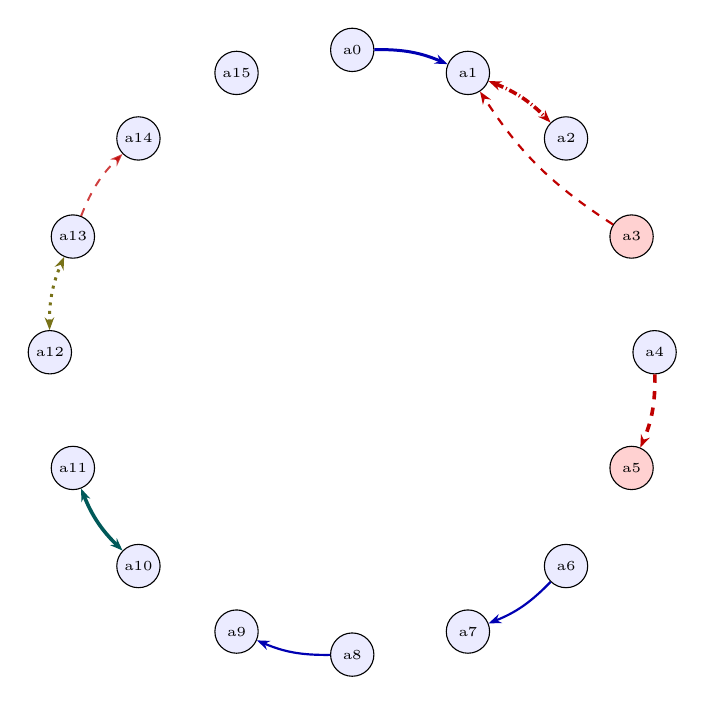
\begin{tikzpicture}[>={Stealth[length=1.6mm]}]
  \node[circle,draw,fill=blue!8,inner sep=1pt,minimum size=5.5mm,font=\tiny] (a0) at (90.0:3.84) {a0};
  \node[circle,draw,fill=blue!8,inner sep=1pt,minimum size=5.5mm,font=\tiny] (a1) at (67.5:3.84) {a1};
  \node[circle,draw,fill=blue!8,inner sep=1pt,minimum size=5.5mm,font=\tiny] (a2) at (45.0:3.84) {a2};
  \node[circle,draw,fill=red!18,inner sep=1pt,minimum size=5.5mm,font=\tiny] (a3) at (22.5:3.84) {a3};
  \node[circle,draw,fill=blue!8,inner sep=1pt,minimum size=5.5mm,font=\tiny] (a4) at (0.0:3.84) {a4};
  \node[circle,draw,fill=red!18,inner sep=1pt,minimum size=5.5mm,font=\tiny] (a5) at (-22.5:3.84) {a5};
  \node[circle,draw,fill=blue!8,inner sep=1pt,minimum size=5.5mm,font=\tiny] (a6) at (-45.0:3.84) {a6};
  \node[circle,draw,fill=blue!8,inner sep=1pt,minimum size=5.5mm,font=\tiny] (a7) at (-67.5:3.84) {a7};
  \node[circle,draw,fill=blue!8,inner sep=1pt,minimum size=5.5mm,font=\tiny] (a8) at (-90.0:3.84) {a8};
  \node[circle,draw,fill=blue!8,inner sep=1pt,minimum size=5.5mm,font=\tiny] (a9) at (-112.5:3.84) {a9};
  \node[circle,draw,fill=blue!8,inner sep=1pt,minimum size=5.5mm,font=\tiny] (a10) at (-135.0:3.84) {a10};
  \node[circle,draw,fill=blue!8,inner sep=1pt,minimum size=5.5mm,font=\tiny] (a11) at (-157.5:3.84) {a11};
  \node[circle,draw,fill=blue!8,inner sep=1pt,minimum size=5.5mm,font=\tiny] (a12) at (-180.0:3.84) {a12};
  \node[circle,draw,fill=blue!8,inner sep=1pt,minimum size=5.5mm,font=\tiny] (a13) at (-202.5:3.84) {a13};
  \node[circle,draw,fill=blue!8,inner sep=1pt,minimum size=5.5mm,font=\tiny] (a14) at (-225.0:3.84) {a14};
  \node[circle,draw,fill=blue!8,inner sep=1pt,minimum size=5.5mm,font=\tiny] (a15) at (-247.5:3.84) {a15};
  \draw[-{Stealth[length=1.6mm]}, blue!70!black, line width=1.08pt] (a0) to[bend left=12] (a1);
  \draw[{Stealth[length=1.6mm]}-{Stealth[length=1.6mm]}, red!75!black, densely dashdotted, line width=1.31pt] (a1) to[bend left=12] (a2);
  \draw[-{Stealth[length=1.6mm]}, red!75!black, dashed, line width=0.79pt] (a3) to[bend left=12] (a1);
  \draw[-{Stealth[length=1.6mm]}, red!75!black, dashed, line width=1.31pt] (a4) to[bend left=12] (a5);
  \draw[-{Stealth[length=1.6mm]}, blue!70!black, line width=0.79pt] (a6) to[bend left=12] (a7);
  \draw[-{Stealth[length=1.6mm]}, blue!70!black, line width=0.79pt] (a8) to[bend left=12] (a9);
  \draw[{Stealth[length=1.6mm]}-{Stealth[length=1.6mm]}, teal!70!black, line width=1.31pt] (a10) to[bend left=12] (a11);
  \draw[{Stealth[length=1.6mm]}-{Stealth[length=1.6mm]}, olive!80!black, dotted, line width=1.08pt] (a12) to[bend left=12] (a13);
  \draw[-{Stealth[length=1.6mm]}, red!75!black, dashed, opacity=0.75, line width=0.71pt] (a13) to[bend left=12] (a14);
\end{tikzpicture}
}
\\[2pt]{\footnotesize all gold edges: 9 factors}
\end{minipage}\hfill\begin{minipage}[t]{0.48\linewidth}\centering
\resizebox{!}{6.4cm}{%
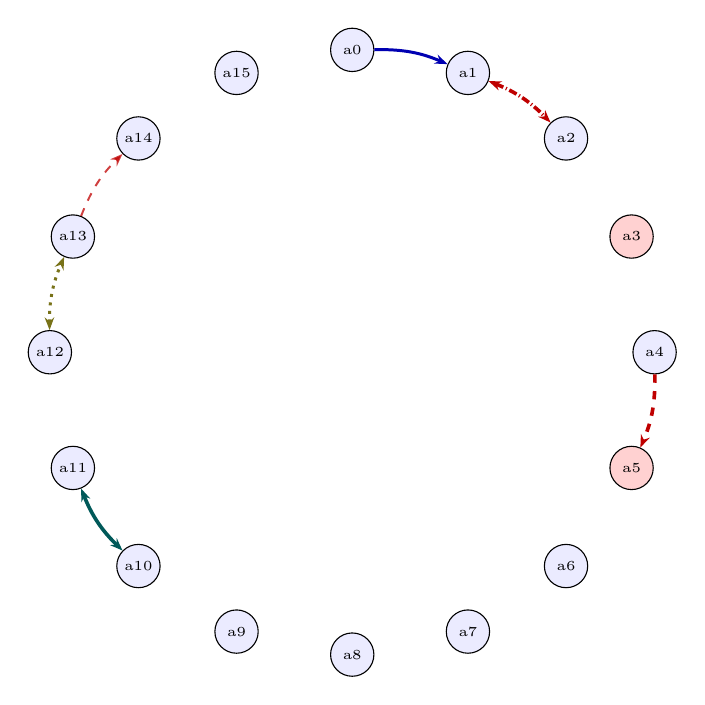
\begin{tikzpicture}[>={Stealth[length=1.6mm]}]
  \node[circle,draw,fill=blue!8,inner sep=1pt,minimum size=5.5mm,font=\tiny] (a0) at (90.0:3.84) {a0};
  \node[circle,draw,fill=blue!8,inner sep=1pt,minimum size=5.5mm,font=\tiny] (a1) at (67.5:3.84) {a1};
  \node[circle,draw,fill=blue!8,inner sep=1pt,minimum size=5.5mm,font=\tiny] (a2) at (45.0:3.84) {a2};
  \node[circle,draw,fill=red!18,inner sep=1pt,minimum size=5.5mm,font=\tiny] (a3) at (22.5:3.84) {a3};
  \node[circle,draw,fill=blue!8,inner sep=1pt,minimum size=5.5mm,font=\tiny] (a4) at (0.0:3.84) {a4};
  \node[circle,draw,fill=red!18,inner sep=1pt,minimum size=5.5mm,font=\tiny] (a5) at (-22.5:3.84) {a5};
  \node[circle,draw,fill=blue!8,inner sep=1pt,minimum size=5.5mm,font=\tiny] (a6) at (-45.0:3.84) {a6};
  \node[circle,draw,fill=blue!8,inner sep=1pt,minimum size=5.5mm,font=\tiny] (a7) at (-67.5:3.84) {a7};
  \node[circle,draw,fill=blue!8,inner sep=1pt,minimum size=5.5mm,font=\tiny] (a8) at (-90.0:3.84) {a8};
  \node[circle,draw,fill=blue!8,inner sep=1pt,minimum size=5.5mm,font=\tiny] (a9) at (-112.5:3.84) {a9};
  \node[circle,draw,fill=blue!8,inner sep=1pt,minimum size=5.5mm,font=\tiny] (a10) at (-135.0:3.84) {a10};
  \node[circle,draw,fill=blue!8,inner sep=1pt,minimum size=5.5mm,font=\tiny] (a11) at (-157.5:3.84) {a11};
  \node[circle,draw,fill=blue!8,inner sep=1pt,minimum size=5.5mm,font=\tiny] (a12) at (-180.0:3.84) {a12};
  \node[circle,draw,fill=blue!8,inner sep=1pt,minimum size=5.5mm,font=\tiny] (a13) at (-202.5:3.84) {a13};
  \node[circle,draw,fill=blue!8,inner sep=1pt,minimum size=5.5mm,font=\tiny] (a14) at (-225.0:3.84) {a14};
  \node[circle,draw,fill=blue!8,inner sep=1pt,minimum size=5.5mm,font=\tiny] (a15) at (-247.5:3.84) {a15};
  \draw[-{Stealth[length=1.6mm]}, blue!70!black, line width=1.08pt] (a0) to[bend left=12] (a1);
  \draw[{Stealth[length=1.6mm]}-{Stealth[length=1.6mm]}, red!75!black, densely dashdotted, line width=1.31pt] (a1) to[bend left=12] (a2);
  \draw[-{Stealth[length=1.6mm]}, red!75!black, dashed, line width=1.31pt] (a4) to[bend left=12] (a5);
  \draw[{Stealth[length=1.6mm]}-{Stealth[length=1.6mm]}, teal!70!black, line width=1.31pt] (a10) to[bend left=12] (a11);
  \draw[{Stealth[length=1.6mm]}-{Stealth[length=1.6mm]}, olive!80!black, dotted, line width=1.08pt] (a12) to[bend left=12] (a13);
  \draw[-{Stealth[length=1.6mm]}, red!75!black, dashed, opacity=0.75, line width=0.71pt] (a13) to[bend left=12] (a14);
\end{tikzpicture}
}
\\[2pt]{\footnotesize valid edges only: 6 factors}
\end{minipage}
\caption{Relation graph for \texttt{locobench-claude-5-fixed-f006-r1}. Nodes are atoms on a circle, tinted red when the item marks them non-factual (prior 0.1) and blue when factual (prior 0.9). Edges are gold relations: solid blue = entailment, dashed red = contradiction, double-headed teal = equivalence, dash-dotted red (double-headed) = exclusive (exactly-one), dotted olive (double-headed) = co-necessity (at-least-one); thickness scales with the factor probability. Ordering-only Precedence edges carry no factor and so are not drawn.}
\label{fig:graph-locobench-claude-5-fixed-f006-r1}
\end{figure}

\begin{table}[htbp]
\centering
\footnotesize
\setlength{\tabcolsep}{3.5pt}
\caption{The specific gold relations of \texttt{locobench-claude-5-fixed-f006-r1}. \textbf{$p$ used} is the factor probability the MRF received: the band midpoint, times $(1-\lambda)$ for a resolved concession, or \emph{none} for an ordering-only edge (no factor). \textbf{Valid} marks the deliberately-planted errors with their kind. \textbf{Res.} is the resolving atom of a resolved concession.}
\label{tab:rels-locobench-claude-5-fixed-f006-r1}
\begin{tabular}{lllllrll}
\toprule
ID & Endpoints & Sense & Coupling & Band & $p$ used & Valid & Res. \\
\midrule
\texttt{r000} & \texttt{a0} $\to$ \texttt{a1} & Evidence & \texttt{entailment} & moderate & 0.720 & \checkmark &  \\
\texttt{r001} & \texttt{a1} $\leftrightarrow$ \texttt{a2} & Alternative & \texttt{exclusive} & strong & 0.925 & \checkmark &  \\
\texttt{r002} & \texttt{a3} $\leftrightarrow$ \texttt{a1} & Contrast & \texttt{contradiction} & weak & 0.470 & $\times$ {\scriptsize false\_endpoint} &  \\
\texttt{r003} & \texttt{a4} $\leftrightarrow$ \texttt{a5} & Contrast & \texttt{contradiction} & strong & 0.925 & \checkmark &  \\
\texttt{r004} & \texttt{a6} $\to$ \texttt{a7} & Evidence & \texttt{entailment} & weak & 0.470 & $\times$ {\scriptsize spurious} &  \\
\texttt{r005} & \texttt{a8} $\to$ \texttt{a9} & Cause-Effect & \texttt{entailment} & weak & 0.470 & $\times$ {\scriptsize wrong\_sense} &  \\
\texttt{r006} & \texttt{a10} $\leftrightarrow$ \texttt{a11} & Restatement & \texttt{equivalence} & strong & 0.925 & \checkmark &  \\
\texttt{r007} & \texttt{a12} $\leftrightarrow$ \texttt{a13} & Disjunction & \texttt{co\_necessity} & moderate & 0.720 & \checkmark &  \\
\texttt{r008} & \texttt{a13} $\to$ \texttt{a14} & Concession & \texttt{contradiction} & moderate & 0.396 & \checkmark & \texttt{a15} \\
\texttt{r009} & \texttt{a0} $\to$ \texttt{a14} & Succession & \texttt{none} & moderate & \emph{none} & $\times$ {\scriptsize wrong\_direction} &  \\
\bottomrule
\end{tabular}
\end{table}

\begin{table}[htbp]
\centering
\footnotesize
\caption{Atoms of \texttt{locobench-claude-5-fixed-f006-r1}: the \texttt{factual} label, the prior it maps to, the posterior marginal $P(a_i{=}1)$ the MRF returns, and the shift. Atoms dragged below their prior are the ones the coherence structure penalises.}
\label{tab:atoms-locobench-claude-5-fixed-f006-r1}
\begin{tabular}{llrrrp{7.2cm}}
\toprule
Atom & fact & $\pi_i$ & $P(a_i{=}1)$ & $\Delta$ & Text \\
\midrule
\texttt{a0} & \checkmark & 0.90 & 0.910 & +0.010 & \footnotesize The iridium anomaly at the Cretaceous–Paleogene boundary was first reported in 1980 by Luis Alvarez and colleagues. \\
\texttt{a1} & \checkmark & 0.90 & 0.800 & -0.100 & \footnotesize The Cretaceous–Paleogene boundary layer is enriched in iridium relative to surrounding strata. \\
\texttt{a2} & \checkmark & 0.90 & 0.535 & -0.365 & \footnotesize The Cretaceous–Paleogene boundary layer shows no iridium enrichment relative to surrounding strata. \\
\texttt{a3} & $\times$ & 0.10 & 0.103 & +0.003 & \footnotesize Iridium is more abundant in Earth's continental crust than in chondritic meteorites. \\
\texttt{a4} & \checkmark & 0.90 & 0.938 & +0.038 & \footnotesize Shocked quartz forms only at the shock pressures generated by hypervelocity impacts. \\
\texttt{a5} & $\times$ & 0.10 & 0.015 & -0.085 & \footnotesize Shocked quartz forms at shock pressures below 0.5 gigapascals. \\
\texttt{a6} & \checkmark & 0.90 & 0.895 & -0.005 & \footnotesize Shocked quartz grains occur in Cretaceous–Paleogene boundary sediments at sites on multiple continents. \\
\texttt{a7} & \checkmark & 0.90 & 0.890 & -0.010 & \footnotesize The Chicxulub crater lies buried beneath the Yucatán Peninsula in Mexico. \\
\texttt{a8} & \checkmark & 0.90 & 0.895 & -0.005 & \footnotesize The Chicxulub crater measures roughly 180 kilometres across. \\
\texttt{a9} & \checkmark & 0.90 & 0.890 & -0.010 & \footnotesize Argon-argon dating of impact glass places the Chicxulub event at about 66 million years ago. \\
\texttt{a10} & \checkmark & 0.90 & 0.979 & +0.079 & \footnotesize The Cretaceous–Paleogene boundary is dated to approximately 66 million years ago. \\
\texttt{a11} & \checkmark & 0.90 & 0.979 & +0.079 & \footnotesize The end-Cretaceous mass extinction took place roughly 66 million years before the present. \\
\texttt{a12} & \checkmark & 0.90 & 0.929 & +0.029 & \footnotesize The Chicxulub impact lofted sulfate aerosols and dust that abruptly darkened and cooled the global atmosphere. \\
\texttt{a13} & \checkmark & 0.90 & 0.939 & +0.039 & \footnotesize Deccan Traps eruptions injected large volumes of sulfur dioxide and carbon dioxide into the atmosphere before the boundary. \\
\texttt{a14} & \checkmark & 0.90 & 0.930 & +0.030 & \footnotesize A 2010 review panel of 41 scientists concluded that the Chicxulub impact triggered the end-Cretaceous mass extinction. \\
\texttt{a15} & \checkmark & 0.90 & 0.900 & +0.000 & \footnotesize The 2010 review determined that Deccan Traps volcanism was not the principal cause of the end-Cretaceous extinction. \\
\bottomrule
\end{tabular}
\end{table}

\subsection{Civil Engineering -- break\_2 (\texttt{locobench-claude-5-fixed-f009-r1})}

\textbf{Topic:} Civil Engineering (Engineering \& Technology). \textbf{Family:} \texttt{f009} (CHAIN), rung 1 (\emph{break\_2}). \textbf{Scores:} mean-marg $= 0.783$, consist $= 0.499$, reified $= 0.319$, log-Z $= 0.277$.



\paragraph{Framing question.} \emph{How do forensic engineers adjudicate between design deficiency and construction workmanship when a newly completed bridge deck develops premature cracking, and what evidence settles the dispute?}



\paragraph{Response.} {\small Adjudicating between design deficiency and defective workmanship on a prematurely cracked deck is a sequential exercise in which each class of evidence narrows the field of admissible explanations. The record ordinarily opens with the chronology of distress. In the case that best illustrates the method, transverse cracks appeared in the bridge deck within six months of opening to traffic; the investigating team produced crack maps recording the orientation, width, and spacing of each crack in the deck. Such mapping is not merely descriptive, because the geometry it captures feeds directly into code classification. Specifically, cracks narrower than 0.10 millimetres are classified as structurally critical under AASHTO provisions, so the widths entered on the map govern whether the distress is treated as a serviceability nuisance or as a matter bearing on load capacity.

Mapping alone cannot distinguish a design shortfall from a construction lapse, and the inquiry therefore moves to the material itself. Forensic engineers extracted concrete cores from the cracked areas of the deck. Cores taken from an in-service deck, by contrast, are inadmissible as forensic evidence under bridge design codes. Petrographic examination of those samples identified microcracking associated with drying shrinkage, a diagnosis reachable only on the condition that cores are removed from the cracked regions in the first place, since the microstructural signature cannot be read from the surface. The observed microcracking indicates that restrained drying shrinkage is a recognised cause of transverse cracking in bridge decks, which is why the petrographic result reorients the inquiry away from flexural overload and toward the interaction of concrete volume change with restraint from the girders and the reinforcing mat.

At that point the parties advance competing accounts of the same mechanism. Although the contractor attributed the cracking to insufficient shrinkage reinforcement in the design, the designer attributed the cracking to premature removal of curing blankets by the contractor. Both accounts are consistent with shrinkage-driven distress, so neither can be preferred on mechanism alone; the discrimination must come from measurements of what was actually built and how it was cured. To that end, ground-penetrating radar surveys located the reinforcing steel and measured concrete cover depth across the affected spans, producing a non-destructive record of the mat's position that can be compared line by line against the contract documents.

The comparison is dispositive in a strict sense, because the possibilities are exhaustive and mutually exclusive: either the as-built reinforcement spacing in the deck matched the approved drawings, or that spacing departed from the approved drawings, and exactly one of these can be true. The dispute review board determined that the as-built reinforcement spacing conformed to the approved drawings — that is, it adopted the first of those two possibilities and treated the radar and core data as showing the mat where the designer had placed it. The board's determination stands in contrast to the departure of the as-built spacing from the approved drawings, and it removed from contention any theory that the steel had been misplaced during construction.

With the reinforcement exonerated, attention turned to the concrete supplied and the curing regime imposed on it, and here the evidence supports at least one of two departures from the specification, perhaps both: the delivered concrete had a water–cement ratio above the specified maximum, and the deck received fewer than the seven days of wet curing required by the specification. Either departure increases free shrinkage and reduces early tensile capacity, and both lie within the contractor's control rather than the designer's. On that footing the court ultimately held that the contractor's curing practice, and not the design, caused the premature cracking, resolving the standoff between the two attributions in favour of the designer's account and confirming that quantified curing and mix-compliance records, coupled with as-built verification of the steel, are what actually settle such disputes.}

\begin{figure}[htbp]
\centering
\begin{minipage}[t]{0.48\linewidth}\centering
\resizebox{!}{6.4cm}{%
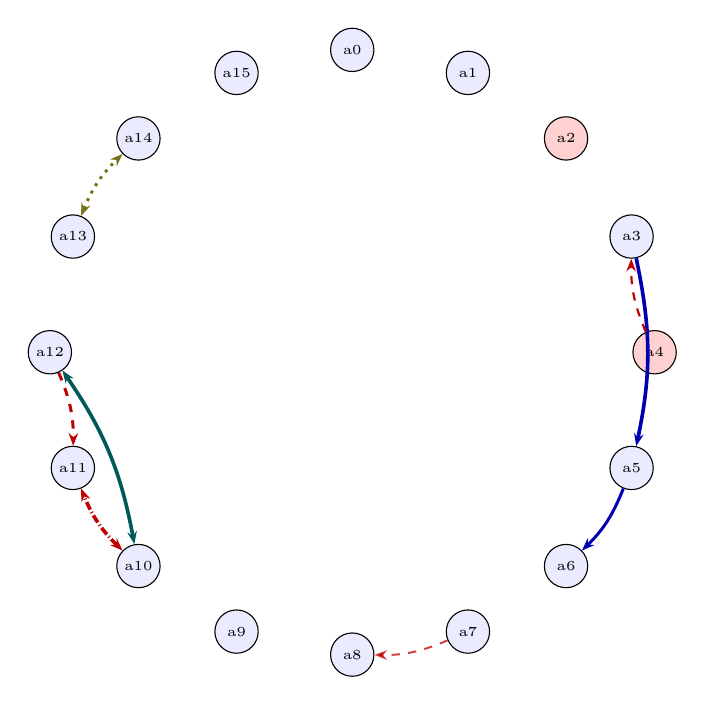
\begin{tikzpicture}[>={Stealth[length=1.6mm]}]
  \node[circle,draw,fill=blue!8,inner sep=1pt,minimum size=5.5mm,font=\tiny] (a0) at (90.0:3.84) {a0};
  \node[circle,draw,fill=blue!8,inner sep=1pt,minimum size=5.5mm,font=\tiny] (a1) at (67.5:3.84) {a1};
  \node[circle,draw,fill=red!18,inner sep=1pt,minimum size=5.5mm,font=\tiny] (a2) at (45.0:3.84) {a2};
  \node[circle,draw,fill=blue!8,inner sep=1pt,minimum size=5.5mm,font=\tiny] (a3) at (22.5:3.84) {a3};
  \node[circle,draw,fill=red!18,inner sep=1pt,minimum size=5.5mm,font=\tiny] (a4) at (0.0:3.84) {a4};
  \node[circle,draw,fill=blue!8,inner sep=1pt,minimum size=5.5mm,font=\tiny] (a5) at (-22.5:3.84) {a5};
  \node[circle,draw,fill=blue!8,inner sep=1pt,minimum size=5.5mm,font=\tiny] (a6) at (-45.0:3.84) {a6};
  \node[circle,draw,fill=blue!8,inner sep=1pt,minimum size=5.5mm,font=\tiny] (a7) at (-67.5:3.84) {a7};
  \node[circle,draw,fill=blue!8,inner sep=1pt,minimum size=5.5mm,font=\tiny] (a8) at (-90.0:3.84) {a8};
  \node[circle,draw,fill=blue!8,inner sep=1pt,minimum size=5.5mm,font=\tiny] (a9) at (-112.5:3.84) {a9};
  \node[circle,draw,fill=blue!8,inner sep=1pt,minimum size=5.5mm,font=\tiny] (a10) at (-135.0:3.84) {a10};
  \node[circle,draw,fill=blue!8,inner sep=1pt,minimum size=5.5mm,font=\tiny] (a11) at (-157.5:3.84) {a11};
  \node[circle,draw,fill=blue!8,inner sep=1pt,minimum size=5.5mm,font=\tiny] (a12) at (-180.0:3.84) {a12};
  \node[circle,draw,fill=blue!8,inner sep=1pt,minimum size=5.5mm,font=\tiny] (a13) at (-202.5:3.84) {a13};
  \node[circle,draw,fill=blue!8,inner sep=1pt,minimum size=5.5mm,font=\tiny] (a14) at (-225.0:3.84) {a14};
  \node[circle,draw,fill=blue!8,inner sep=1pt,minimum size=5.5mm,font=\tiny] (a15) at (-247.5:3.84) {a15};
  \draw[-{Stealth[length=1.6mm]}, blue!70!black, line width=1.31pt] (a3) to[bend left=12] (a5);
  \draw[-{Stealth[length=1.6mm]}, red!75!black, dashed, line width=0.79pt] (a4) to[bend left=12] (a3);
  \draw[-{Stealth[length=1.6mm]}, blue!70!black, line width=1.08pt] (a5) to[bend left=12] (a6);
  \draw[-{Stealth[length=1.6mm]}, red!75!black, dashed, opacity=0.75, line width=0.71pt] (a7) to[bend left=12] (a8);
  \draw[{Stealth[length=1.6mm]}-{Stealth[length=1.6mm]}, red!75!black, densely dashdotted, line width=1.31pt] (a10) to[bend left=12] (a11);
  \draw[{Stealth[length=1.6mm]}-{Stealth[length=1.6mm]}, teal!70!black, line width=1.31pt] (a12) to[bend left=12] (a10);
  \draw[-{Stealth[length=1.6mm]}, red!75!black, dashed, line width=1.08pt] (a12) to[bend left=12] (a11);
  \draw[{Stealth[length=1.6mm]}-{Stealth[length=1.6mm]}, olive!80!black, dotted, line width=1.08pt] (a13) to[bend left=12] (a14);
\end{tikzpicture}
}
\\[2pt]{\footnotesize all gold edges: 8 factors}
\end{minipage}\hfill\begin{minipage}[t]{0.48\linewidth}\centering
\resizebox{!}{6.4cm}{%
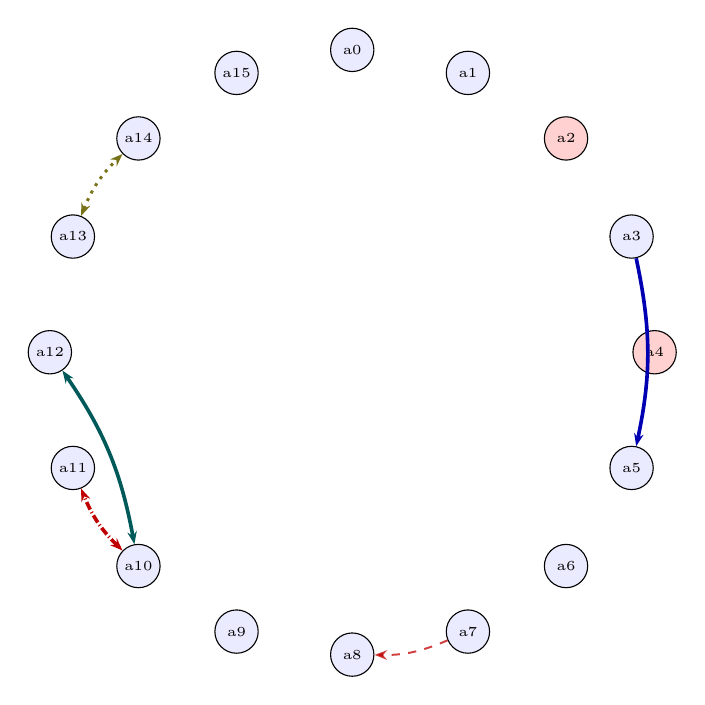
\begin{tikzpicture}[>={Stealth[length=1.6mm]}]
  \node[circle,draw,fill=blue!8,inner sep=1pt,minimum size=5.5mm,font=\tiny] (a0) at (90.0:3.84) {a0};
  \node[circle,draw,fill=blue!8,inner sep=1pt,minimum size=5.5mm,font=\tiny] (a1) at (67.5:3.84) {a1};
  \node[circle,draw,fill=red!18,inner sep=1pt,minimum size=5.5mm,font=\tiny] (a2) at (45.0:3.84) {a2};
  \node[circle,draw,fill=blue!8,inner sep=1pt,minimum size=5.5mm,font=\tiny] (a3) at (22.5:3.84) {a3};
  \node[circle,draw,fill=red!18,inner sep=1pt,minimum size=5.5mm,font=\tiny] (a4) at (0.0:3.84) {a4};
  \node[circle,draw,fill=blue!8,inner sep=1pt,minimum size=5.5mm,font=\tiny] (a5) at (-22.5:3.84) {a5};
  \node[circle,draw,fill=blue!8,inner sep=1pt,minimum size=5.5mm,font=\tiny] (a6) at (-45.0:3.84) {a6};
  \node[circle,draw,fill=blue!8,inner sep=1pt,minimum size=5.5mm,font=\tiny] (a7) at (-67.5:3.84) {a7};
  \node[circle,draw,fill=blue!8,inner sep=1pt,minimum size=5.5mm,font=\tiny] (a8) at (-90.0:3.84) {a8};
  \node[circle,draw,fill=blue!8,inner sep=1pt,minimum size=5.5mm,font=\tiny] (a9) at (-112.5:3.84) {a9};
  \node[circle,draw,fill=blue!8,inner sep=1pt,minimum size=5.5mm,font=\tiny] (a10) at (-135.0:3.84) {a10};
  \node[circle,draw,fill=blue!8,inner sep=1pt,minimum size=5.5mm,font=\tiny] (a11) at (-157.5:3.84) {a11};
  \node[circle,draw,fill=blue!8,inner sep=1pt,minimum size=5.5mm,font=\tiny] (a12) at (-180.0:3.84) {a12};
  \node[circle,draw,fill=blue!8,inner sep=1pt,minimum size=5.5mm,font=\tiny] (a13) at (-202.5:3.84) {a13};
  \node[circle,draw,fill=blue!8,inner sep=1pt,minimum size=5.5mm,font=\tiny] (a14) at (-225.0:3.84) {a14};
  \node[circle,draw,fill=blue!8,inner sep=1pt,minimum size=5.5mm,font=\tiny] (a15) at (-247.5:3.84) {a15};
  \draw[-{Stealth[length=1.6mm]}, blue!70!black, line width=1.31pt] (a3) to[bend left=12] (a5);
  \draw[-{Stealth[length=1.6mm]}, red!75!black, dashed, opacity=0.75, line width=0.71pt] (a7) to[bend left=12] (a8);
  \draw[{Stealth[length=1.6mm]}-{Stealth[length=1.6mm]}, red!75!black, densely dashdotted, line width=1.31pt] (a10) to[bend left=12] (a11);
  \draw[{Stealth[length=1.6mm]}-{Stealth[length=1.6mm]}, teal!70!black, line width=1.31pt] (a12) to[bend left=12] (a10);
  \draw[{Stealth[length=1.6mm]}-{Stealth[length=1.6mm]}, olive!80!black, dotted, line width=1.08pt] (a13) to[bend left=12] (a14);
\end{tikzpicture}
}
\\[2pt]{\footnotesize valid edges only: 5 factors}
\end{minipage}
\caption{Relation graph for \texttt{locobench-claude-5-fixed-f009-r1}. Nodes are atoms on a circle, tinted red when the item marks them non-factual (prior 0.1) and blue when factual (prior 0.9). Edges are gold relations: solid blue = entailment, dashed red = contradiction, double-headed teal = equivalence, dash-dotted red (double-headed) = exclusive (exactly-one), dotted olive (double-headed) = co-necessity (at-least-one); thickness scales with the factor probability. Ordering-only Precedence edges carry no factor and so are not drawn.}
\label{fig:graph-locobench-claude-5-fixed-f009-r1}
\end{figure}

\begin{table}[htbp]
\centering
\footnotesize
\setlength{\tabcolsep}{3.5pt}
\caption{The specific gold relations of \texttt{locobench-claude-5-fixed-f009-r1}. \textbf{$p$ used} is the factor probability the MRF received: the band midpoint, times $(1-\lambda)$ for a resolved concession, or \emph{none} for an ordering-only edge (no factor). \textbf{Valid} marks the deliberately-planted errors with their kind. \textbf{Res.} is the resolving atom of a resolved concession.}
\label{tab:rels-locobench-claude-5-fixed-f009-r1}
\begin{tabular}{lllllrll}
\toprule
ID & Endpoints & Sense & Coupling & Band & $p$ used & Valid & Res. \\
\midrule
\texttt{r002} & \texttt{a3} $\to$ \texttt{a5} & Condition & \texttt{entailment} & strong & 0.925 & \checkmark &  \\
\texttt{r003} & \texttt{a4} $\leftrightarrow$ \texttt{a3} & Contrast & \texttt{contradiction} & weak & 0.470 & $\times$ {\scriptsize spurious} &  \\
\texttt{r004} & \texttt{a5} $\to$ \texttt{a6} & Evidence & \texttt{entailment} & moderate & 0.720 & $\times$ {\scriptsize wrong\_direction} &  \\
\texttt{r005} & \texttt{a7} $\to$ \texttt{a8} & Concession & \texttt{contradiction} & moderate & 0.396 & \checkmark & \texttt{a15} \\
\texttt{r006} & \texttt{a10} $\leftrightarrow$ \texttt{a11} & Alternative & \texttt{exclusive} & strong & 0.925 & \checkmark &  \\
\texttt{r007} & \texttt{a12} $\leftrightarrow$ \texttt{a10} & Restatement & \texttt{equivalence} & strong & 0.925 & \checkmark &  \\
\texttt{r008} & \texttt{a12} $\leftrightarrow$ \texttt{a11} & Contrast & \texttt{contradiction} & moderate & 0.720 & $\times$ {\scriptsize wrong\_sense} &  \\
\texttt{r009} & \texttt{a13} $\leftrightarrow$ \texttt{a14} & Disjunction & \texttt{co\_necessity} & moderate & 0.720 & \checkmark &  \\
\bottomrule
\end{tabular}
\end{table}

\begin{table}[htbp]
\centering
\footnotesize
\caption{Atoms of \texttt{locobench-claude-5-fixed-f009-r1}: the \texttt{factual} label, the prior it maps to, the posterior marginal $P(a_i{=}1)$ the MRF returns, and the shift. Atoms dragged below their prior are the ones the coherence structure penalises.}
\label{tab:atoms-locobench-claude-5-fixed-f009-r1}
\begin{tabular}{llrrrp{7.2cm}}
\toprule
Atom & fact & $\pi_i$ & $P(a_i{=}1)$ & $\Delta$ & Text \\
\midrule
\texttt{a0} & \checkmark & 0.90 & 0.900 & +0.000 & \footnotesize Transverse cracks appeared in the bridge deck within six months of opening to traffic. \\
\texttt{a1} & \checkmark & 0.90 & 0.900 & +0.000 & \footnotesize Crack maps recorded the orientation, width, and spacing of each crack in the deck. \\
\texttt{a2} & $\times$ & 0.10 & 0.100 & +0.000 & \footnotesize Cracks narrower than 0.10 millimetres are classified as structurally critical under AASHTO provisions. \\
\texttt{a3} & \checkmark & 0.90 & 0.940 & +0.040 & \footnotesize Forensic engineers extracted concrete cores from the cracked areas of the deck. \\
\texttt{a4} & $\times$ & 0.10 & 0.105 & +0.005 & \footnotesize Cores taken from an in-service deck are inadmissible as forensic evidence under bridge design codes. \\
\texttt{a5} & \checkmark & 0.90 & 0.989 & +0.089 & \footnotesize Petrographic examination of the cores identified microcracking associated with drying shrinkage. \\
\texttt{a6} & \checkmark & 0.90 & 0.958 & +0.058 & \footnotesize Restrained drying shrinkage is a recognised cause of transverse cracking in bridge decks. \\
\texttt{a7} & \checkmark & 0.90 & 0.913 & +0.013 & \footnotesize The contractor attributed the cracking to insufficient shrinkage reinforcement in the design. \\
\texttt{a8} & \checkmark & 0.90 & 0.929 & +0.029 & \footnotesize The designer attributed the cracking to premature removal of curing blankets by the contractor. \\
\texttt{a9} & \checkmark & 0.90 & 0.900 & +0.000 & \footnotesize Ground-penetrating radar surveys located the reinforcing steel and measured concrete cover depth. \\
\texttt{a10} & \checkmark & 0.90 & 0.922 & +0.022 & \footnotesize The as-built reinforcement spacing in the deck matched the approved drawings. \\
\texttt{a11} & \checkmark & 0.90 & 0.283 & -0.617 & \footnotesize The as-built reinforcement spacing in the deck departed from the approved drawings. \\
\texttt{a12} & \checkmark & 0.90 & 0.937 & +0.037 & \footnotesize The dispute review board determined that the as-built reinforcement spacing conformed to the approved drawings. \\
\texttt{a13} & \checkmark & 0.90 & 0.929 & +0.029 & \footnotesize The delivered concrete had a water-cement ratio above the specified maximum. \\
\texttt{a14} & \checkmark & 0.90 & 0.929 & +0.029 & \footnotesize The deck received fewer than the seven days of wet curing required by the specification. \\
\texttt{a15} & \checkmark & 0.90 & 0.900 & +0.000 & \footnotesize The court ultimately held that the contractor's curing practice, and not the design, caused the premature cracking. \\
\bottomrule
\end{tabular}
\end{table}

\subsection{Cybersecurity -- base (\texttt{locobench-claude-5-fixed-f012-r1})}

\textbf{Topic:} Cybersecurity (Engineering \& Technology). \textbf{Family:} \texttt{f012} (CONFLICT), rung 1 (\emph{base}). \textbf{Scores:} mean-marg $= 0.789$, consist $= 0.397$, reified $= 0.185$, log-Z $= 0.370$.



\paragraph{Framing question.} \emph{How do incident responders establish whether a data breach originated from a compromised insider credential or an external exploitation of an unpatched system when the victim organization and its security vendor advance conflicting accounts?}



\paragraph{Response.} {\small When a victim organization and its security vendor advance incompatible accounts of the same
intrusion, the responder's task is not to arbitrate between narratives but to test each against
artefacts whose generation is independent of either party's interest. In the case that best
illustrates the method, although the security vendor's report attributed the intrusion to misuse of
a stolen employee credential, the organization attributed the intrusion to exploitation of an
unpatched remote access appliance. Each account implies a different initial access vector and
therefore a different set of expected traces: credential misuse predicts anomalous authentication
events unaccompanied by process execution on the perimeter device, whereas exploitation predicts
writes to that device's own file system.

Resolution began with governance rather than technique. The organization retained an independent
digital forensics firm to investigate the breach, and only after that engagement was in place did
investigators reconstruct an intrusion timeline from VPN authentication logs, firewall netflow
records, and endpoint telemetry. A timeline assembled from three independently maintained streams
constrains both hypotheses, since a misread or altered entry in one source will not be corroborated
by the other two. Configuration evidence was collected alongside the log evidence. Investigators
compared the appliance's firmware build number against the manufacturer's patched release, and that
comparison confirms that the remote access appliance was missing the manufacturer's security patch
at the time of the intrusion. What the artefacts supported at this stage was a disjunction rather
than a verdict: at least one of two conditions obtained — that unpatched exposure, or the use of an
employee's valid credentials by an unauthorized party to access the network — and perhaps both.

Two further findings sharpened the picture. A web shell was recovered from the appliance's file
system; by contrast, multi-factor authentication was not enforced on the remote access portal. The
web shell is the more diagnostic of the two, because such an artefact cannot be produced by
authentication alone: it requires the ability to write executable content to the appliance, which
in turn requires a code-execution flaw in the exposed service. Its presence therefore raises the
prior probability of the exploitation account without yet excluding concurrent credential abuse,
since an attacker who has established a foothold on a perimeter device is well positioned to harvest
the credentials that traverse it.

The absence of a second factor is to say, equivalently, that the remote access portal accepted
logins using only a username and a password. That configuration matters for the evidentiary
weighting rather than for attribution as such, because it means an authentication record showing a
valid credential is compatible with either a legitimate user or any party in possession of the
password. Attribution of the earliest activity turned on a further observation: the use of an
employee's valid credentials by an unauthorized party indicates that the employee whose account was
used was on approved leave during the earliest unauthorized access, a fact corroborated by human
resources records rather than by the network itself. Windows Event ID 4625, on the other hand,
records successful interactive logons.

Framework mapping was applied to the reconstructed sequence in order to express it in terms
comparable across incidents. MITRE ATT\&CK technique T1078 covers exploitation of public-facing
applications, and the categories it defines are what allow a regulator to compare one organization's
account with another's. The scope question was settled on the same evidentiary basis as the vector
question: either no customer records were exfiltrated from the environment, or approximately 2.4
million customer records were exfiltrated from it; the two cannot both be true, and one of them must
hold. The regulator ultimately determined that the intrusion began with exploitation of the
unpatched appliance — a specific instance of that technique, and the determination that settles the
tension between the two competing attributions with which the matter opened. The methodological
lesson is that conflicting accounts are adjudicated not by weighing the parties' credibility but by
identifying which artefacts each hypothesis requires, and then establishing whether those artefacts
exist.}

\begin{figure}[htbp]
\centering
\begin{minipage}[t]{0.48\linewidth}\centering
\resizebox{!}{6.4cm}{%
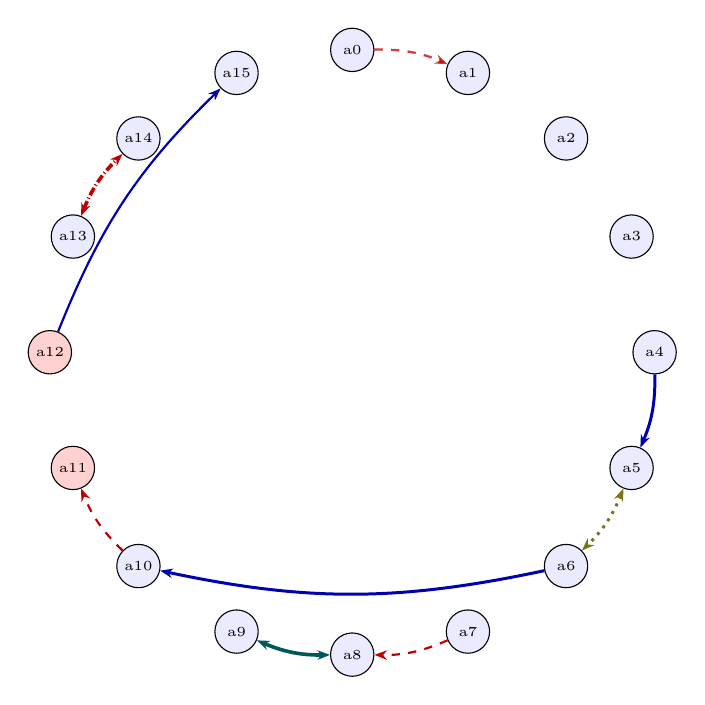
\begin{tikzpicture}[>={Stealth[length=1.6mm]}]
  \node[circle,draw,fill=blue!8,inner sep=1pt,minimum size=5.5mm,font=\tiny] (a0) at (90.0:3.84) {a0};
  \node[circle,draw,fill=blue!8,inner sep=1pt,minimum size=5.5mm,font=\tiny] (a1) at (67.5:3.84) {a1};
  \node[circle,draw,fill=blue!8,inner sep=1pt,minimum size=5.5mm,font=\tiny] (a2) at (45.0:3.84) {a2};
  \node[circle,draw,fill=blue!8,inner sep=1pt,minimum size=5.5mm,font=\tiny] (a3) at (22.5:3.84) {a3};
  \node[circle,draw,fill=blue!8,inner sep=1pt,minimum size=5.5mm,font=\tiny] (a4) at (0.0:3.84) {a4};
  \node[circle,draw,fill=blue!8,inner sep=1pt,minimum size=5.5mm,font=\tiny] (a5) at (-22.5:3.84) {a5};
  \node[circle,draw,fill=blue!8,inner sep=1pt,minimum size=5.5mm,font=\tiny] (a6) at (-45.0:3.84) {a6};
  \node[circle,draw,fill=blue!8,inner sep=1pt,minimum size=5.5mm,font=\tiny] (a7) at (-67.5:3.84) {a7};
  \node[circle,draw,fill=blue!8,inner sep=1pt,minimum size=5.5mm,font=\tiny] (a8) at (-90.0:3.84) {a8};
  \node[circle,draw,fill=blue!8,inner sep=1pt,minimum size=5.5mm,font=\tiny] (a9) at (-112.5:3.84) {a9};
  \node[circle,draw,fill=blue!8,inner sep=1pt,minimum size=5.5mm,font=\tiny] (a10) at (-135.0:3.84) {a10};
  \node[circle,draw,fill=red!18,inner sep=1pt,minimum size=5.5mm,font=\tiny] (a11) at (-157.5:3.84) {a11};
  \node[circle,draw,fill=red!18,inner sep=1pt,minimum size=5.5mm,font=\tiny] (a12) at (-180.0:3.84) {a12};
  \node[circle,draw,fill=blue!8,inner sep=1pt,minimum size=5.5mm,font=\tiny] (a13) at (-202.5:3.84) {a13};
  \node[circle,draw,fill=blue!8,inner sep=1pt,minimum size=5.5mm,font=\tiny] (a14) at (-225.0:3.84) {a14};
  \node[circle,draw,fill=blue!8,inner sep=1pt,minimum size=5.5mm,font=\tiny] (a15) at (-247.5:3.84) {a15};
  \draw[-{Stealth[length=1.6mm]}, red!75!black, dashed, opacity=0.75, line width=0.84pt] (a0) to[bend left=12] (a1);
  \draw[-{Stealth[length=1.6mm]}, blue!70!black, line width=1.08pt] (a4) to[bend left=12] (a5);
  \draw[{Stealth[length=1.6mm]}-{Stealth[length=1.6mm]}, olive!80!black, dotted, line width=1.08pt] (a5) to[bend left=12] (a6);
  \draw[-{Stealth[length=1.6mm]}, blue!70!black, line width=1.08pt] (a6) to[bend left=12] (a10);
  \draw[-{Stealth[length=1.6mm]}, red!75!black, dashed, line width=0.79pt] (a7) to[bend left=12] (a8);
  \draw[{Stealth[length=1.6mm]}-{Stealth[length=1.6mm]}, teal!70!black, line width=1.31pt] (a8) to[bend left=12] (a9);
  \draw[-{Stealth[length=1.6mm]}, red!75!black, dashed, line width=0.79pt] (a10) to[bend left=12] (a11);
  \draw[-{Stealth[length=1.6mm]}, blue!70!black, line width=0.79pt] (a12) to[bend left=12] (a15);
  \draw[{Stealth[length=1.6mm]}-{Stealth[length=1.6mm]}, red!75!black, densely dashdotted, line width=1.31pt] (a13) to[bend left=12] (a14);
\end{tikzpicture}
}
\\[2pt]{\footnotesize all gold edges: 9 factors}
\end{minipage}\hfill\begin{minipage}[t]{0.48\linewidth}\centering
\resizebox{!}{6.4cm}{%
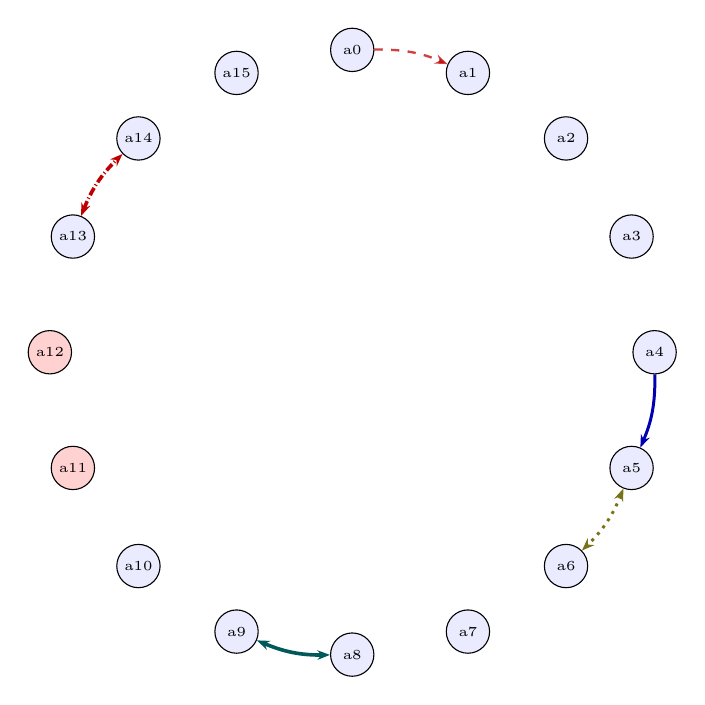
\begin{tikzpicture}[>={Stealth[length=1.6mm]}]
  \node[circle,draw,fill=blue!8,inner sep=1pt,minimum size=5.5mm,font=\tiny] (a0) at (90.0:3.84) {a0};
  \node[circle,draw,fill=blue!8,inner sep=1pt,minimum size=5.5mm,font=\tiny] (a1) at (67.5:3.84) {a1};
  \node[circle,draw,fill=blue!8,inner sep=1pt,minimum size=5.5mm,font=\tiny] (a2) at (45.0:3.84) {a2};
  \node[circle,draw,fill=blue!8,inner sep=1pt,minimum size=5.5mm,font=\tiny] (a3) at (22.5:3.84) {a3};
  \node[circle,draw,fill=blue!8,inner sep=1pt,minimum size=5.5mm,font=\tiny] (a4) at (0.0:3.84) {a4};
  \node[circle,draw,fill=blue!8,inner sep=1pt,minimum size=5.5mm,font=\tiny] (a5) at (-22.5:3.84) {a5};
  \node[circle,draw,fill=blue!8,inner sep=1pt,minimum size=5.5mm,font=\tiny] (a6) at (-45.0:3.84) {a6};
  \node[circle,draw,fill=blue!8,inner sep=1pt,minimum size=5.5mm,font=\tiny] (a7) at (-67.5:3.84) {a7};
  \node[circle,draw,fill=blue!8,inner sep=1pt,minimum size=5.5mm,font=\tiny] (a8) at (-90.0:3.84) {a8};
  \node[circle,draw,fill=blue!8,inner sep=1pt,minimum size=5.5mm,font=\tiny] (a9) at (-112.5:3.84) {a9};
  \node[circle,draw,fill=blue!8,inner sep=1pt,minimum size=5.5mm,font=\tiny] (a10) at (-135.0:3.84) {a10};
  \node[circle,draw,fill=red!18,inner sep=1pt,minimum size=5.5mm,font=\tiny] (a11) at (-157.5:3.84) {a11};
  \node[circle,draw,fill=red!18,inner sep=1pt,minimum size=5.5mm,font=\tiny] (a12) at (-180.0:3.84) {a12};
  \node[circle,draw,fill=blue!8,inner sep=1pt,minimum size=5.5mm,font=\tiny] (a13) at (-202.5:3.84) {a13};
  \node[circle,draw,fill=blue!8,inner sep=1pt,minimum size=5.5mm,font=\tiny] (a14) at (-225.0:3.84) {a14};
  \node[circle,draw,fill=blue!8,inner sep=1pt,minimum size=5.5mm,font=\tiny] (a15) at (-247.5:3.84) {a15};
  \draw[-{Stealth[length=1.6mm]}, red!75!black, dashed, opacity=0.75, line width=0.84pt] (a0) to[bend left=12] (a1);
  \draw[-{Stealth[length=1.6mm]}, blue!70!black, line width=1.08pt] (a4) to[bend left=12] (a5);
  \draw[{Stealth[length=1.6mm]}-{Stealth[length=1.6mm]}, olive!80!black, dotted, line width=1.08pt] (a5) to[bend left=12] (a6);
  \draw[{Stealth[length=1.6mm]}-{Stealth[length=1.6mm]}, teal!70!black, line width=1.31pt] (a8) to[bend left=12] (a9);
  \draw[{Stealth[length=1.6mm]}-{Stealth[length=1.6mm]}, red!75!black, densely dashdotted, line width=1.31pt] (a13) to[bend left=12] (a14);
\end{tikzpicture}
}
\\[2pt]{\footnotesize valid edges only: 5 factors}
\end{minipage}
\caption{Relation graph for \texttt{locobench-claude-5-fixed-f012-r1}. Nodes are atoms on a circle, tinted red when the item marks them non-factual (prior 0.1) and blue when factual (prior 0.9). Edges are gold relations: solid blue = entailment, dashed red = contradiction, double-headed teal = equivalence, dash-dotted red (double-headed) = exclusive (exactly-one), dotted olive (double-headed) = co-necessity (at-least-one); thickness scales with the factor probability. Ordering-only Precedence edges carry no factor and so are not drawn.}
\label{fig:graph-locobench-claude-5-fixed-f012-r1}
\end{figure}

\begin{table}[htbp]
\centering
\footnotesize
\setlength{\tabcolsep}{3.5pt}
\caption{The specific gold relations of \texttt{locobench-claude-5-fixed-f012-r1}. \textbf{$p$ used} is the factor probability the MRF received: the band midpoint, times $(1-\lambda)$ for a resolved concession, or \emph{none} for an ordering-only edge (no factor). \textbf{Valid} marks the deliberately-planted errors with their kind. \textbf{Res.} is the resolving atom of a resolved concession.}
\label{tab:rels-locobench-claude-5-fixed-f012-r1}
\begin{tabular}{lllllrll}
\toprule
ID & Endpoints & Sense & Coupling & Band & $p$ used & Valid & Res. \\
\midrule
\texttt{r000} & \texttt{a0} $\to$ \texttt{a1} & Concession & \texttt{contradiction} & strong & 0.509 & \checkmark & \texttt{a15} \\
\texttt{r001} & \texttt{a2} $\to$ \texttt{a3} & Precedence & \texttt{none} & moderate & \emph{none} & \checkmark &  \\
\texttt{r002} & \texttt{a4} $\to$ \texttt{a5} & Evidence & \texttt{entailment} & moderate & 0.720 & \checkmark &  \\
\texttt{r003} & \texttt{a5} $\leftrightarrow$ \texttt{a6} & Disjunction & \texttt{co\_necessity} & moderate & 0.720 & \checkmark &  \\
\texttt{r004} & \texttt{a6} $\to$ \texttt{a10} & Evidence & \texttt{entailment} & moderate & 0.720 & $\times$ {\scriptsize wrong\_direction} &  \\
\texttt{r005} & \texttt{a7} $\leftrightarrow$ \texttt{a8} & Contrast & \texttt{contradiction} & weak & 0.470 & $\times$ {\scriptsize spurious} &  \\
\texttt{r006} & \texttt{a8} $\leftrightarrow$ \texttt{a9} & Restatement & \texttt{equivalence} & strong & 0.925 & \checkmark &  \\
\texttt{r007} & \texttt{a10} $\leftrightarrow$ \texttt{a11} & Contrast & \texttt{contradiction} & weak & 0.470 & $\times$ {\scriptsize false\_endpoint} &  \\
\texttt{r008} & \texttt{a12} $\to$ \texttt{a15} & Instantiation & \texttt{entailment} & weak & 0.470 & $\times$ {\scriptsize false\_endpoint} &  \\
\texttt{r009} & \texttt{a13} $\leftrightarrow$ \texttt{a14} & Alternative & \texttt{exclusive} & strong & 0.925 & \checkmark &  \\
\bottomrule
\end{tabular}
\end{table}

\begin{table}[htbp]
\centering
\footnotesize
\caption{Atoms of \texttt{locobench-claude-5-fixed-f012-r1}: the \texttt{factual} label, the prior it maps to, the posterior marginal $P(a_i{=}1)$ the MRF returns, and the shift. Atoms dragged below their prior are the ones the coherence structure penalises.}
\label{tab:atoms-locobench-claude-5-fixed-f012-r1}
\begin{tabular}{llrrrp{7.2cm}}
\toprule
Atom & fact & $\pi_i$ & $P(a_i{=}1)$ & $\Delta$ & Text \\
\midrule
\texttt{a0} & \checkmark & 0.90 & 0.899 & -0.001 & \footnotesize The security vendor's report attributed the intrusion to misuse of a stolen employee credential. \\
\texttt{a1} & \checkmark & 0.90 & 0.897 & -0.003 & \footnotesize The organization attributed the intrusion to exploitation of an unpatched remote access appliance. \\
\texttt{a2} & \checkmark & 0.90 & 0.900 & +0.000 & \footnotesize The organization retained an independent digital forensics firm to investigate the breach. \\
\texttt{a3} & \checkmark & 0.90 & 0.900 & +0.000 & \footnotesize Investigators reconstructed an intrusion timeline from VPN authentication logs, firewall netflow records, and endpoint telemetry. \\
\texttt{a4} & \checkmark & 0.90 & 0.925 & +0.025 & \footnotesize Investigators compared the appliance's firmware build number against the manufacturer's patched release. \\
\texttt{a5} & \checkmark & 0.90 & 0.968 & +0.068 & \footnotesize The remote access appliance was missing the manufacturer's security patch at the time of the intrusion. \\
\texttt{a6} & \checkmark & 0.90 & 0.946 & +0.046 & \footnotesize An employee's valid credentials were used by an unauthorized party to access the network. \\
\texttt{a7} & \checkmark & 0.90 & 0.905 & +0.005 & \footnotesize A web shell was recovered from the appliance's file system. \\
\texttt{a8} & \checkmark & 0.90 & 0.981 & +0.081 & \footnotesize Multi-factor authentication was not enforced on the remote access portal. \\
\texttt{a9} & \checkmark & 0.90 & 0.980 & +0.080 & \footnotesize The remote access portal accepted logins using only a username and a password. \\
\texttt{a10} & \checkmark & 0.90 & 0.953 & +0.053 & \footnotesize The employee whose account was used was on approved leave during the earliest unauthorized access. \\
\texttt{a11} & $\times$ & 0.10 & 0.111 & +0.011 & \footnotesize Windows Event ID 4625 records successful interactive logons. \\
\texttt{a12} & $\times$ & 0.10 & 0.096 & -0.004 & \footnotesize MITRE ATT\&CK technique T1078 covers exploitation of public-facing applications. \\
\texttt{a13} & \checkmark & 0.90 & 0.632 & -0.268 & \footnotesize No customer records were exfiltrated from the environment. \\
\texttt{a14} & \checkmark & 0.90 & 0.632 & -0.268 & \footnotesize Approximately 2.4 million customer records were exfiltrated from the environment. \\
\texttt{a15} & \checkmark & 0.90 & 0.899 & -0.001 & \footnotesize The regulator ultimately determined that the intrusion began with exploitation of the unpatched appliance. \\
\bottomrule
\end{tabular}
\end{table}

\subsection{Economics -- base (\texttt{locobench-claude-5-fixed-f013-r1})}

\textbf{Topic:} Economics (Social Sciences). \textbf{Family:} \texttt{f013} (CONFLICT), rung 1 (\emph{base}). \textbf{Scores:} mean-marg $= 0.741$, consist $= 0.824$, reified $= 0.387$, log-Z $= 0.360$.



\paragraph{Framing question.} \emph{How do economists adjudicate between the claim that the 2021–2023 inflation surge originated in pandemic-era supply disruptions versus the claim that it originated in excessive fiscal and monetary stimulus?}



\paragraph{Response.} {\small Adjudicating between a supply-side and a demand-side origin for the 2021–2023 inflation surge is an exercise in attributing a single price movement to two candidate impulses that arrived at nearly the same moment. The fiscal impulse is the easier of the two to date and to size: the American Rescue Plan Act of March 2021 authorized roughly \$1.9 trillion in fiscal support, and Lawrence Summers had warned a month earlier, in February 2021, that the stimulus package risked igniting inflationary pressures. That the warning preceded the legislation matters methodologically, since it establishes the demand-side hypothesis as a prior commitment rather than an ex post rationalization of prices already observed.

The monetary leg of the same account is measured on a different series. The US M2 money supply grew by roughly 25 percent during 2020, an expansion without parallel in the postwar record. Because that \$1.9 trillion authorization routed cash directly into household accounts, pandemic-era fiscal transfers lifted US household goods demand above its pre-pandemic trend in 2021, and the sharp growth of the money stock produced the same overshoot in goods purchases. A demand overshoot is not, however, sufficient to characterize the 2021 goods market on its own. At least one of two conditions obtained in that year, and perhaps both: the overshoot in household goods demand, or pandemic-era logistics bottlenecks that constrained the volume of goods that could be delivered to US buyers.

Quantitative evidence on the constraint side is comparatively direct. The New York Fed's Global Supply Chain Pressure Index reached its record high in December 2021, which indicates that logistics frictions were binding on deliverable volumes precisely when consumer prices were accelerating most sharply. Global container freight spot rates, on the other hand, remained flat throughout 2021. The measurement difficulty extends to the price series itself, where the two readings in circulation for the peak cannot both be true and one of them must hold: either US headline CPI inflation exceeded 9 percent year over year at some point during 2022, or it remained below 9 percent year over year throughout that year.

Formal decomposition is what allows the dispute to be settled rather than merely restated. Adam Shapiro of the San Francisco Fed developed a method that labels each spending category's inflation as supply-driven or demand-driven from the co-movement of prices and quantities, on the reasoning that a category whose price rises while its quantity falls is being pushed by supply rather than pulled by demand. Applied to the first year of the surge, that procedure indicates that roughly half of the above-target inflation in 2021 stemmed from supply-side factors; equivalently, supply-driven components accounted for about 50 percent of the excess inflation recorded in 2021. The Bernanke–Blanchard analysis concluded that a wage-price spiral drove the initial 2021 inflation surge, even though that 50 percent supply share had been documented for the same twelve months. The tension is settled in favor of the decomposition by the IMF's 2023 World Economic Outlook, which concluded that supply shocks accounted for the majority of the initial inflation surge in advanced economies, leaving wage dynamics as a propagation mechanism rather than an originating one.

The monetary-policy timeline is where the demand-side account remains most exposed. The Federal Reserve began lifting its policy rate from the effective lower bound in March 2021; its own official policy review, by contrast, determined that the federal funds rate remained at the effective lower bound until March 2022. Which dating is adopted bears directly on the verdict, since a central bank holding rates at zero through the year of fastest price acceleration carries a different share of responsibility than one already tightening at the outset. The resolution most economists now defend is accordingly compositional rather than exclusive: supply constraints dominate the 2021 acceleration, whereas the persistence of inflation through 2022 and 2023, concentrated in services and shelter, is better explained by demand that stimulus had elevated and that policy was slow to restrain.}

\begin{figure}[htbp]
\centering
\begin{minipage}[t]{0.48\linewidth}\centering
\resizebox{!}{6.4cm}{%
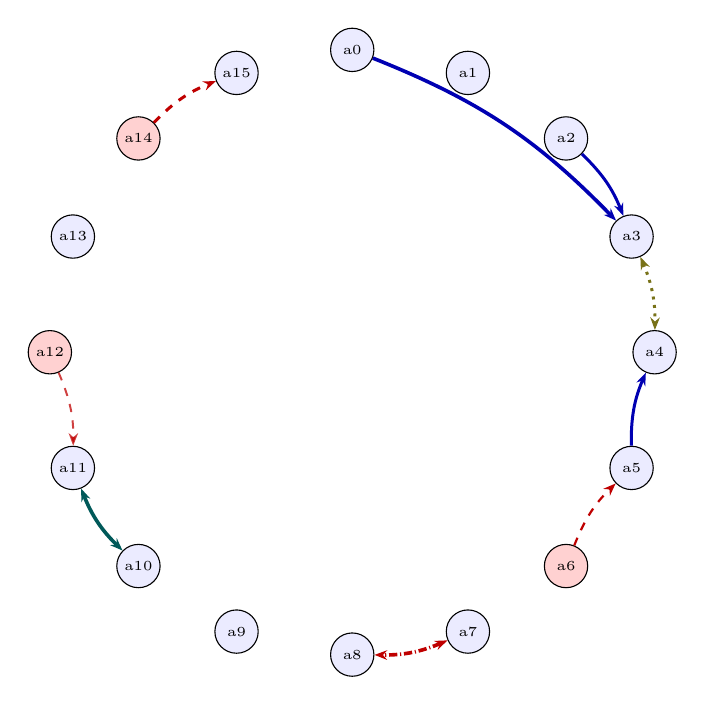
\begin{tikzpicture}[>={Stealth[length=1.6mm]}]
  \node[circle,draw,fill=blue!8,inner sep=1pt,minimum size=5.5mm,font=\tiny] (a0) at (90.0:3.84) {a0};
  \node[circle,draw,fill=blue!8,inner sep=1pt,minimum size=5.5mm,font=\tiny] (a1) at (67.5:3.84) {a1};
  \node[circle,draw,fill=blue!8,inner sep=1pt,minimum size=5.5mm,font=\tiny] (a2) at (45.0:3.84) {a2};
  \node[circle,draw,fill=blue!8,inner sep=1pt,minimum size=5.5mm,font=\tiny] (a3) at (22.5:3.84) {a3};
  \node[circle,draw,fill=blue!8,inner sep=1pt,minimum size=5.5mm,font=\tiny] (a4) at (0.0:3.84) {a4};
  \node[circle,draw,fill=blue!8,inner sep=1pt,minimum size=5.5mm,font=\tiny] (a5) at (-22.5:3.84) {a5};
  \node[circle,draw,fill=red!18,inner sep=1pt,minimum size=5.5mm,font=\tiny] (a6) at (-45.0:3.84) {a6};
  \node[circle,draw,fill=blue!8,inner sep=1pt,minimum size=5.5mm,font=\tiny] (a7) at (-67.5:3.84) {a7};
  \node[circle,draw,fill=blue!8,inner sep=1pt,minimum size=5.5mm,font=\tiny] (a8) at (-90.0:3.84) {a8};
  \node[circle,draw,fill=blue!8,inner sep=1pt,minimum size=5.5mm,font=\tiny] (a9) at (-112.5:3.84) {a9};
  \node[circle,draw,fill=blue!8,inner sep=1pt,minimum size=5.5mm,font=\tiny] (a10) at (-135.0:3.84) {a10};
  \node[circle,draw,fill=blue!8,inner sep=1pt,minimum size=5.5mm,font=\tiny] (a11) at (-157.5:3.84) {a11};
  \node[circle,draw,fill=red!18,inner sep=1pt,minimum size=5.5mm,font=\tiny] (a12) at (-180.0:3.84) {a12};
  \node[circle,draw,fill=blue!8,inner sep=1pt,minimum size=5.5mm,font=\tiny] (a13) at (-202.5:3.84) {a13};
  \node[circle,draw,fill=red!18,inner sep=1pt,minimum size=5.5mm,font=\tiny] (a14) at (-225.0:3.84) {a14};
  \node[circle,draw,fill=blue!8,inner sep=1pt,minimum size=5.5mm,font=\tiny] (a15) at (-247.5:3.84) {a15};
  \draw[-{Stealth[length=1.6mm]}, blue!70!black, line width=1.31pt] (a0) to[bend left=12] (a3);
  \draw[-{Stealth[length=1.6mm]}, blue!70!black, line width=1.08pt] (a2) to[bend left=12] (a3);
  \draw[{Stealth[length=1.6mm]}-{Stealth[length=1.6mm]}, olive!80!black, dotted, line width=1.08pt] (a3) to[bend left=12] (a4);
  \draw[-{Stealth[length=1.6mm]}, blue!70!black, line width=1.08pt] (a5) to[bend left=12] (a4);
  \draw[-{Stealth[length=1.6mm]}, red!75!black, dashed, line width=0.79pt] (a6) to[bend left=12] (a5);
  \draw[{Stealth[length=1.6mm]}-{Stealth[length=1.6mm]}, red!75!black, densely dashdotted, line width=1.31pt] (a7) to[bend left=12] (a8);
  \draw[{Stealth[length=1.6mm]}-{Stealth[length=1.6mm]}, teal!70!black, line width=1.31pt] (a10) to[bend left=12] (a11);
  \draw[-{Stealth[length=1.6mm]}, red!75!black, dashed, opacity=0.75, line width=0.71pt] (a12) to[bend left=12] (a11);
  \draw[-{Stealth[length=1.6mm]}, red!75!black, dashed, line width=1.08pt] (a14) to[bend left=12] (a15);
\end{tikzpicture}
}
\\[2pt]{\footnotesize all gold edges: 9 factors}
\end{minipage}\hfill\begin{minipage}[t]{0.48\linewidth}\centering
\resizebox{!}{6.4cm}{%
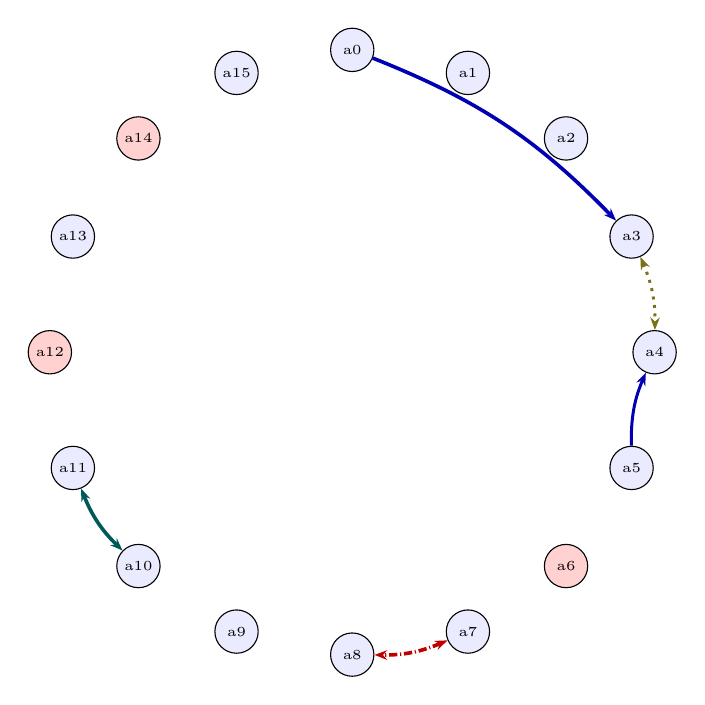
\begin{tikzpicture}[>={Stealth[length=1.6mm]}]
  \node[circle,draw,fill=blue!8,inner sep=1pt,minimum size=5.5mm,font=\tiny] (a0) at (90.0:3.84) {a0};
  \node[circle,draw,fill=blue!8,inner sep=1pt,minimum size=5.5mm,font=\tiny] (a1) at (67.5:3.84) {a1};
  \node[circle,draw,fill=blue!8,inner sep=1pt,minimum size=5.5mm,font=\tiny] (a2) at (45.0:3.84) {a2};
  \node[circle,draw,fill=blue!8,inner sep=1pt,minimum size=5.5mm,font=\tiny] (a3) at (22.5:3.84) {a3};
  \node[circle,draw,fill=blue!8,inner sep=1pt,minimum size=5.5mm,font=\tiny] (a4) at (0.0:3.84) {a4};
  \node[circle,draw,fill=blue!8,inner sep=1pt,minimum size=5.5mm,font=\tiny] (a5) at (-22.5:3.84) {a5};
  \node[circle,draw,fill=red!18,inner sep=1pt,minimum size=5.5mm,font=\tiny] (a6) at (-45.0:3.84) {a6};
  \node[circle,draw,fill=blue!8,inner sep=1pt,minimum size=5.5mm,font=\tiny] (a7) at (-67.5:3.84) {a7};
  \node[circle,draw,fill=blue!8,inner sep=1pt,minimum size=5.5mm,font=\tiny] (a8) at (-90.0:3.84) {a8};
  \node[circle,draw,fill=blue!8,inner sep=1pt,minimum size=5.5mm,font=\tiny] (a9) at (-112.5:3.84) {a9};
  \node[circle,draw,fill=blue!8,inner sep=1pt,minimum size=5.5mm,font=\tiny] (a10) at (-135.0:3.84) {a10};
  \node[circle,draw,fill=blue!8,inner sep=1pt,minimum size=5.5mm,font=\tiny] (a11) at (-157.5:3.84) {a11};
  \node[circle,draw,fill=red!18,inner sep=1pt,minimum size=5.5mm,font=\tiny] (a12) at (-180.0:3.84) {a12};
  \node[circle,draw,fill=blue!8,inner sep=1pt,minimum size=5.5mm,font=\tiny] (a13) at (-202.5:3.84) {a13};
  \node[circle,draw,fill=red!18,inner sep=1pt,minimum size=5.5mm,font=\tiny] (a14) at (-225.0:3.84) {a14};
  \node[circle,draw,fill=blue!8,inner sep=1pt,minimum size=5.5mm,font=\tiny] (a15) at (-247.5:3.84) {a15};
  \draw[-{Stealth[length=1.6mm]}, blue!70!black, line width=1.31pt] (a0) to[bend left=12] (a3);
  \draw[{Stealth[length=1.6mm]}-{Stealth[length=1.6mm]}, olive!80!black, dotted, line width=1.08pt] (a3) to[bend left=12] (a4);
  \draw[-{Stealth[length=1.6mm]}, blue!70!black, line width=1.08pt] (a5) to[bend left=12] (a4);
  \draw[{Stealth[length=1.6mm]}-{Stealth[length=1.6mm]}, red!75!black, densely dashdotted, line width=1.31pt] (a7) to[bend left=12] (a8);
  \draw[{Stealth[length=1.6mm]}-{Stealth[length=1.6mm]}, teal!70!black, line width=1.31pt] (a10) to[bend left=12] (a11);
\end{tikzpicture}
}
\\[2pt]{\footnotesize valid edges only: 5 factors}
\end{minipage}
\caption{Relation graph for \texttt{locobench-claude-5-fixed-f013-r1}. Nodes are atoms on a circle, tinted red when the item marks them non-factual (prior 0.1) and blue when factual (prior 0.9). Edges are gold relations: solid blue = entailment, dashed red = contradiction, double-headed teal = equivalence, dash-dotted red (double-headed) = exclusive (exactly-one), dotted olive (double-headed) = co-necessity (at-least-one); thickness scales with the factor probability. Ordering-only Precedence edges carry no factor and so are not drawn.}
\label{fig:graph-locobench-claude-5-fixed-f013-r1}
\end{figure}

\begin{table}[htbp]
\centering
\footnotesize
\setlength{\tabcolsep}{3.5pt}
\caption{The specific gold relations of \texttt{locobench-claude-5-fixed-f013-r1}. \textbf{$p$ used} is the factor probability the MRF received: the band midpoint, times $(1-\lambda)$ for a resolved concession, or \emph{none} for an ordering-only edge (no factor). \textbf{Valid} marks the deliberately-planted errors with their kind. \textbf{Res.} is the resolving atom of a resolved concession.}
\label{tab:rels-locobench-claude-5-fixed-f013-r1}
\begin{tabular}{lllllrll}
\toprule
ID & Endpoints & Sense & Coupling & Band & $p$ used & Valid & Res. \\
\midrule
\texttt{r000} & \texttt{a1} $\to$ \texttt{a0} & Precedence & \texttt{none} & moderate & \emph{none} & \checkmark &  \\
\texttt{r001} & \texttt{a0} $\to$ \texttt{a3} & Cause-Effect & \texttt{entailment} & strong & 0.925 & \checkmark &  \\
\texttt{r002} & \texttt{a2} $\to$ \texttt{a3} & Cause-Effect & \texttt{entailment} & moderate & 0.720 & $\times$ {\scriptsize wrong\_sense} &  \\
\texttt{r003} & \texttt{a3} $\leftrightarrow$ \texttt{a4} & Disjunction & \texttt{co\_necessity} & moderate & 0.720 & \checkmark &  \\
\texttt{r004} & \texttt{a5} $\to$ \texttt{a4} & Evidence & \texttt{entailment} & moderate & 0.720 & \checkmark &  \\
\texttt{r005} & \texttt{a6} $\leftrightarrow$ \texttt{a5} & Contrast & \texttt{contradiction} & weak & 0.470 & $\times$ {\scriptsize false\_endpoint} &  \\
\texttt{r006} & \texttt{a7} $\leftrightarrow$ \texttt{a8} & Alternative & \texttt{exclusive} & strong & 0.925 & \checkmark &  \\
\texttt{r007} & \texttt{a10} $\leftrightarrow$ \texttt{a11} & Restatement & \texttt{equivalence} & strong & 0.925 & \checkmark &  \\
\texttt{r008} & \texttt{a12} $\to$ \texttt{a11} & Concession & \texttt{contradiction} & moderate & 0.396 & $\times$ {\scriptsize false\_endpoint} & \texttt{a13} \\
\texttt{r009} & \texttt{a14} $\leftrightarrow$ \texttt{a15} & Contrast & \texttt{contradiction} & moderate & 0.720 & $\times$ {\scriptsize false\_endpoint} &  \\
\bottomrule
\end{tabular}
\end{table}

\begin{table}[htbp]
\centering
\footnotesize
\caption{Atoms of \texttt{locobench-claude-5-fixed-f013-r1}: the \texttt{factual} label, the prior it maps to, the posterior marginal $P(a_i{=}1)$ the MRF returns, and the shift. Atoms dragged below their prior are the ones the coherence structure penalises.}
\label{tab:atoms-locobench-claude-5-fixed-f013-r1}
\begin{tabular}{llrrrp{7.2cm}}
\toprule
Atom & fact & $\pi_i$ & $P(a_i{=}1)$ & $\Delta$ & Text \\
\midrule
\texttt{a0} & \checkmark & 0.90 & 0.942 & +0.042 & \footnotesize The American Rescue Plan Act of March 2021 authorized roughly \$1.9 trillion in fiscal support. \\
\texttt{a1} & \checkmark & 0.90 & 0.900 & +0.000 & \footnotesize Lawrence Summers warned in February 2021 that the stimulus package risked igniting inflationary pressures. \\
\texttt{a2} & \checkmark & 0.90 & 0.928 & +0.028 & \footnotesize The US M2 money supply grew by roughly 25 percent during 2020. \\
\texttt{a3} & \checkmark & 0.90 & 0.996 & +0.096 & \footnotesize Pandemic-era fiscal transfers lifted US household goods demand above its pre-pandemic trend in 2021. \\
\texttt{a4} & \checkmark & 0.90 & 0.968 & +0.068 & \footnotesize Pandemic-era logistics bottlenecks constrained the volume of goods that could be delivered to US buyers in 2021. \\
\texttt{a5} & \checkmark & 0.90 & 0.926 & +0.026 & \footnotesize The New York Fed's Global Supply Chain Pressure Index reached its record high in December 2021. \\
\texttt{a6} & $\times$ & 0.10 & 0.105 & +0.005 & \footnotesize Global container freight spot rates remained flat throughout 2021. \\
\texttt{a7} & \checkmark & 0.90 & 0.632 & -0.268 & \footnotesize US headline CPI inflation exceeded 9 percent year over year at some point during 2022. \\
\texttt{a8} & \checkmark & 0.90 & 0.632 & -0.268 & \footnotesize US headline CPI inflation remained below 9 percent year over year throughout 2022. \\
\texttt{a9} & \checkmark & 0.90 & 0.900 & +0.000 & \footnotesize Adam Shapiro of the San Francisco Fed developed a method that labels each spending category's inflation as supply-driven or demand-driven from the co-movement of prices and quantities. \\
\texttt{a10} & \checkmark & 0.90 & 0.980 & +0.080 & \footnotesize Roughly half of the above-target inflation in 2021 stemmed from supply-side factors. \\
\texttt{a11} & \checkmark & 0.90 & 0.980 & +0.080 & \footnotesize Supply-driven components accounted for about 50 percent of the excess inflation recorded in 2021. \\
\texttt{a12} & $\times$ & 0.10 & 0.118 & +0.018 & \footnotesize The Bernanke–Blanchard analysis concluded that a wage-price spiral drove the initial 2021 inflation surge. \\
\texttt{a13} & \checkmark & 0.90 & 0.900 & +0.000 & \footnotesize The IMF's 2023 World Economic Outlook concluded that supply shocks accounted for the majority of the initial inflation surge in advanced economies. \\
\texttt{a14} & $\times$ & 0.10 & 0.067 & -0.033 & \footnotesize The Federal Reserve began lifting its policy rate from the effective lower bound in March 2021. \\
\texttt{a15} & \checkmark & 0.90 & 0.892 & -0.008 & \footnotesize The Federal Reserve's official policy review determined that the federal funds rate remained at the effective lower bound until March 2022. \\
\bottomrule
\end{tabular}
\end{table}

\section{Findings}

\begin{itemize}
\item \textbf{Every rung carries its own gold relations, so the ladder is a real test.} On the \texttt{gold} arm 167 of 202 ordering assertions hold across all families (\texttt{consist} 54/62, \texttt{mean-marg} 57/70, \texttt{log-Z} 56/70). Because each rung's labels describe the response that ships with them, these pass rates are evidence about the readouts rather than about the corpus --- which is what the previous generation of this dataset could not provide.
\item \textbf{The readouts differ sharply in sensitivity.} Across the 70 scored items \texttt{mean\_marginal} spans only $[0.734, 0.837]$, while \texttt{consistency} spans $[0.357, 0.860]$. With atom priors pinned at $0.9/0.1$ the mean marginal is dominated by those priors and moves little; the conflict-sensitive readouts are what register the contradiction structure. For a benchmark whose families vary conflict structure, \texttt{consistency} and \texttt{log\_partition} are the discriminating readouts.
\item \textbf{The planted invalid relations carry most of the incoherence.} Dropping them changes \texttt{consistency} by -0.031 to 0.415 across items. The planted errors are largely conflict edges anchored to a false endpoint, so they add active contradictions, and the intended-correct subgraph is markedly more coherent. That the effect runs in this direction is a sanity check that the gold labels and the MRF encoding agree about which edges are the damaging ones.
\item \textbf{Relation counts and factor counts are not the same number.} Of 670 gold relations, 67 are Precedence edges that couple no truth values and never reach the MRF, and 262 are deliberately invalid. Any comparison of graph density needs both figures; Table~\ref{tab:dataset} reports them separately for that reason.
\item \textbf{Recovering the graph is harder than scoring it.} The best mined arm (\texttt{bidirectional}) reaches 96.5\% recall at the pair level but only 88.4\% once the Level-1 coupling has to match, at 22.4\% precision. The gold arms show the readouts behave correctly on a correct graph; these numbers are what the pipeline actually delivers from prose, and the gap between the two is the finding.
\item \textbf{The direction split is a policy property, not a model property.} \texttt{windowed} 71.1\% forward vs 21.9\% backward; \texttt{bidirectional} 79.9\% forward vs 76.2\% backward; \texttt{windowed} 82.1\% forward vs 29.5\% backward; \texttt{bidirectional} 89.0\% forward vs 85.7\% backward. A forward-only policy cannot emit a backward ordered pair at all, so its backward recall is bounded by the undirected couplings it can still match on the unordered pair. Any comparison of the two policies' coupling recall is therefore partly a comparison of their reach.
\item \textbf{One policy scores a denser network than the others.} Duplicate unordered pairs: \texttt{windowed} 0, \texttt{bidirectional} 1020. Because edges are not deduplicated, each duplicate puts a second factor on the same variable pair, so that pair's influence is applied twice. Readout differences between the policies cannot be attributed to coverage alone.
\item \textbf{The declared negatives are a cleaner precision signal than the unlabelled pairs.} Violations of the item's own \texttt{non\_relations}: \texttt{windowed} 34/342, \texttt{bidirectional} 119/342, \texttt{windowed} 38/342, \texttt{bidirectional} 147/342. Precision against every unlabelled pair is dominated by pairs of unknown status, whereas these are pairs the corpus asserts are unrelated.
\item \textbf{The type confidence is saturated, so the factor probability is carrying only the strength.} 8179 of 8345 mined relations (98.0\%) have $P(\tau \mid a_i,a_j) = 1.0$, with a minimum of 0.438 across the whole sweep. Because $p = P(\tau \mid a_i,a_j) \times P(a_j \mid a_i,\tau)$, the edge weight is effectively the conditional strength alone. This is a genuine reading and not a missing-logprobs fallback --- that path returns 0.5, not 1.0 --- but it means Prompt~A contributes a label and no usable uncertainty on this model, and the two-factor decomposition is not being exercised. A model whose \texttt{[coupling=...]} span is less peaked, or a calibrator fitted on that span, would be needed to test it.
\item \textbf{The mined numbers are not built on dropped calls.} 0 of 26771 LLM calls failed across the mined arms. This matters because a failed call is parsed as \emph{no relation} --- indistinguishable from a genuine negative --- so an unmeasured failure rate would silently depress recall and inflate every readout. The run refuses a cell whose failure rate exceeds the configured ceiling.
\end{itemize}

\section{Threats to validity}

\begin{itemize}
\item \textbf{Gold relations are labels, not measurements.} The factor probability is a band midpoint, so a \texttt{strong} edge enters at exactly 0.925 whatever the underlying text supports. The gold arms therefore evaluate the MRF encoding and the readouts \emph{given} perfect relation labels. They are the reference point the mined arms are measured against, not a mining result in themselves.
\item \textbf{Two families is a small sample.} The dataset has 14 families over 70 items, all generated by one model. The spreads quoted above describe this dataset; no significance claim is made or implied.
\item \textbf{The ladder tests the readouts, not the miner.} Gold relations vary per rung, so the ordering constraints are a real test --- but of the MRF encoding and the readouts given perfect labels. A live system also has to \emph{recover} those relations from the text, and nothing here measures that.
\item \textbf{The concession discount is applied from the label.} Using the item's \texttt{resolver\_atom\_id} bypasses the text heuristic a live miner must use, so the resolved-concession behaviour shown here is the best case for that mechanism.
\item \textbf{Inference is approximate in general.} Merlin runs weighted mini-bucket at a finite $i$-bound. On these 16-atom networks the induced width is small enough that it reports exact inference, but the normalized log-partition also depends on a MAP floor and a contradiction-free ceiling, so it is the readout most sensitive to any approximation.
\item \textbf{The policy comparison is not a coverage ablation.} \texttt{windowed} and \texttt{all\_pairs} differ in three ways at once: which pairs they reach, whether they consider both directions, and --- because duplicate edges are not merged --- how dense a network they build. A readout difference between them cannot be attributed to coverage alone. Isolating coverage would need one policy at two window radii.
\item \textbf{A failed call and a genuine negative look the same.} The miner parses a captured exception as \emph{no relation}. This run counts those failures and refuses a cell that exceeds a threshold, so the reported numbers are not built on dropped calls --- but the underlying ambiguity is a property of the pipeline, and a run without that accounting would show no symptom.
\item \textbf{The mined figures here are coupling-level, and an earlier revision of this report was not.} Pair level asks only whether two atoms were seen as related; the coupling is what builds the factor, and it is roughly 17 F1 points stricter on this corpus. Any mining number quoted without its match level is ambiguous enough to mislead --- this one did.
\item \textbf{Neither the model's confidence nor a degree cap can filter these relations.} Measured on this corpus, AUC(strength, true-positive) is at or below chance and $P(\tau \mid a_i,a_j)$ is saturated near 1.0 for almost every relation, so every probability threshold tested LOWERED F1 monotonically --- the model is most confident on its most inferential false positives. A per-atom degree cap also lowered F1 at every setting, despite the gold graph being a near-matching: gold's sparsity is a property of which pairs are related, not a budget per atom. Both are recorded here so neither is re-proposed.
\item \textbf{Atom text cannot be located in the response, so character-offset provenance is not available.} The atoms are decontextualized rewrites: across this corpus essentially none occur verbatim in the response and only about a quarter match after whitespace and case normalization. A cited evidence span is checkable only because it is quoted FROM the response, which is literal source text --- the asymmetry the evidence requirement rests on.
\item \textbf{One mined observation per cell, and the sampling noise is not small.} Mining is sampled once per (item, arm) at the model's default temperature. Two independent sweeps of this same configuration were run during development: coupling-level recall was stable to within $0.02$, but the ladder pass rate for one arm moved by $3$ of $28$ assertions --- larger than the gap between several of the arms in Table~\ref{tab:ladder-by-arm}. Treat the ordering of arms whose pass rates differ by only a few assertions as unresolved; the large gap to the gold arm is the robust part.
\end{itemize}

\end{document}
